\documentclass{article}
% Packages nécessaires
% knitr

\usepackage[]{graphicx}
\usepackage[]{color}
\makeatletter
\def\maxwidth{ %
  \ifdim\Gin@nat@width>\linewidth
    \linewidth
  \else
    \Gin@nat@width
  \fi
}
\makeatother

\definecolor{fgcolor}{rgb}{0.345, 0.345, 0.345}
\newcommand{\hlnum}[1]{\textcolor[rgb]{0.686,0.059,0.569}{#1}}%
\newcommand{\hlstr}[1]{\textcolor[rgb]{0.192,0.494,0.8}{#1}}%
\newcommand{\hlcom}[1]{\textcolor[rgb]{0.678,0.584,0.686}{\textit{#1}}}%
\newcommand{\hlopt}[1]{\textcolor[rgb]{0,0,0}{#1}}%
\newcommand{\hlstd}[1]{\textcolor[rgb]{0.345,0.345,0.345}{#1}}%
\newcommand{\hlkwa}[1]{\textcolor[rgb]{0.161,0.373,0.58}{\textbf{#1}}}%
\newcommand{\hlkwb}[1]{\textcolor[rgb]{0.69,0.353,0.396}{#1}}%
\newcommand{\hlkwc}[1]{\textcolor[rgb]{0.333,0.667,0.333}{#1}}%
\newcommand{\hlkwd}[1]{\textcolor[rgb]{0.737,0.353,0.396}{\textbf{#1}}}%

\usepackage{framed}
\makeatletter
\newenvironment{kframe}{%
 \def\at@end@of@kframe{}%
 \ifinner\ifhmode%
  \def\at@end@of@kframe{\end{minipage}}%
  \begin{minipage}{\columnwidth}%
 \fi\fi%
 \def\FrameCommand##1{\hskip\@totalleftmargin \hskip-\fboxsep
 \colorbox{shadecolor}{##1}\hskip-\fboxsep
     % There is no \\@totalrightmargin, so:
     \hskip-\linewidth \hskip-\@totalleftmargin \hskip\columnwidth}%
 \MakeFramed {\advance\hsize-\width
   \@totalleftmargin\z@ \linewidth\hsize
   \@setminipage}}%
 {\par\unskip\endMakeFramed%
 \at@end@of@kframe}
\makeatother

%	\usepackage{knitr}
	
\definecolor{shadecolor}{rgb}{.97, .97, .97}
\definecolor{messagecolor}{rgb}{0, 0, 0}
\definecolor{warningcolor}{rgb}{1, 0, 1}
\definecolor{errorcolor}{rgb}{1, 0, 0}
\newenvironment{knitrout}{}{} % an empty environment to be redefined in TeX
%fin knitr
	
\usepackage{alltt}	

	
	
	\usepackage{ifthen}
	
	
	
% Pour les documents en francais...
	\usepackage[latin1]{inputenc}
	\usepackage[french]{babel}
	\usepackage[french]{varioref}

% Math�matiques
	\usepackage{amsmath}

% Caracteres speciaux suppl�mentaires
	\usepackage{latexsym,amsfonts}

% A documenter
	\usepackage{moreverb}

% Macros pour les paquets
	\usepackage{array}  			% N�cessaires pour les tableaux de la macro Excel.
	\usepackage{dcolumn}
	
% Outil suppl�mentaire pour les tableaux
	\usepackage{multirow}
	\usepackage{booktabs}
%	\usepackage{xcolor} % alternating row colors in table, incompatible avec certains modules
	\usepackage{longtable}
	\usepackage{colortbl}

% Pour ins�rer des graphiques
	\usepackage{graphicx} 			% Graphique simples
	\usepackage{subfigure}			% Graphiques multiples

% Pour ins�rer des couleurs
	\usepackage{color}

% Rotation des objets et des pages
%	\usepackage{rotating}
%	\usepackage{lscape}

% Pour insrer du code source, LaTeX ou SAS par exemple.
	\usepackage{verbatim}
	\usepackage{listings}
	\usepackage{fancyvrb}

%	\lstset{language=SAS,numbers=left}		% Par dfaut le listing est en SAS

% Pour ins�rer des hyperliens
  \usepackage{hyperref}

% American Psychological Association (for bibliographic references).
	\usepackage{apacite}

% Pour l'utilisation des macros
	\usepackage{xspace}

% Pour l'utilisation de notes en fin de document.
%	\usepackage{endnotes}

% Array
%	\usepackage{multirow}
%	\usepackage{booktabs}

% Rotation
%	\usepackage{rotating}

% En t�tes et pieds de pages
	\usepackage{fancyhdr}
	\usepackage{lastpage}
	
	



% Macros commandes



% Pour insérer des dessins de Linux
\newcommand{\LinuxA}{\includegraphics[height=0.5cm]{Graphiques/linux.png}}
\newcommand{\LinuxB}{\includegraphics[height=0.5cm]{Graphiques/linux.png}\xspace}


% Macro pour les petits dessins pour les diff�rents OS.
\newcommand{\Windows}{\emph{Windows}\xspace}
\newcommand{\Mac}{\emph{Mac OS X}\xspace}
\newcommand{\Linux}{\emph{Linux}\xspace}
\newcommand{\MikTeX}{MiK\tex\xspace}

\newcommand{\df}{\emph{data.frame}\xspace}
\newcommand{\dfs}{\emph{data.frames}\xspace}
\newcommand{\liste}{\emph{list}\xspace}
\newcommand{\listes}{\emph{lists}\xspace}

\newcommand{\factor}{\emph{factor}\xspace}
\newcommand{\character}{\emph{character}\xspace}
\newcommand{\logical}{\emph{logical}\xspace}

\newcommand{\cad}{c'est-�-dire\xspace}

\newcommand{\hreff}[2]{\underline{\href{#1}{#2}\xspace}}

% Des raccourcis pour les commandes \LaTeX, \TeX, ...
\newcommand{\latex}{\LaTeX\xspace}
\newcommand{\latexe}{\LaTeXe\xspace}
\newcommand{\tex}{\TeX\xspace}

\newcommand{\indexcom}[1]{\index{#1@\textsl{#1}}}
  
\newcommand{\R}{
\includegraphics[scale=0.025]{Rlogo}}
\newcommand{\licence}{\includegraphics[scale=0.4]{licence}}
  
%\makeatletter
%
%\renewcommand\section{\@startsection {section}{1}{\z@}%
%   {-3.5ex \@plus -1ex \@minus -.2ex}%
%   {2.3ex \@plus.2ex}%
%   {\normalfont\Large\bfseries\textcolor{blue}}}
%   
%\renewcommand\subsection{\@startsection{subsection}{2}{\z@}%
%   {-3.25ex\@plus -1ex \@minus -.2ex}%
%   {1.5ex \@plus .2ex}%
%   {\normalfont\large\bfseries\textcolor{blue}}}
%   
%\renewcommand\subsubsection{\@startsection{subsubsection}{2}{\z@}%
%   {-3.25ex\@plus -1ex \@minus -.2ex}%
%   {1.5ex \@plus .2ex}%
%   {\normalfont\large\bfseries\textcolor{blue}}}
%
%\def\hlinewd#1{%
%\noalign{\ifnum0=`}\fi\hrule \@height #1 %
%\futurelet\reserved@a\@xhline}
%
%\makeatother

 % Définition de l'auteur, ...
% Titre  	 
        \title{Introduction � \R\\Journee}
        \author{Pascal Bessonneau}
				\date{05/2016}

% Pieds de page, marges, ...
% page layout

% By LaTeX commands
%\setlength{\oddsidemargin}{0cm}
%\setlength{\textwidth}{16cm}
%\setlength{\textheight}{24cm}
%\setlength{\topmargin}{-1cm}
%\setlength{\marginparsep}{0.2cm}

% fancyheader parameters
\pagestyle{fancy}  

\fancyfoot[L]{{\small Formation \R}}
\fancyfoot[c]{} 
\fancyfoot[R]{{\small \thepage/\pageref{LastPage}}}

\fancyhead[L]{} 
\fancyhead[c]{}
\fancyhead[R]{} 

\begin{document}
\maketitle
\newpage
\tableofcontents
\newpage
\section{A not so short history of R}

  \subsection{A not so short history of R}
  
% Table generated by Excel2LaTeX from sheet 'Feuil1'
\begin{table}[htbp]
  \centering
  \scalebox{0.6}{
    \begin{tabular}{crl}
    \toprule
    \textbf{version} & \multicolumn{1}{c}{\textbf{Date}} & \multicolumn{1}{c}{\textbf{Description}} \\
    \midrule
    \textbf{0.49} & 1997 & La cr�ation du Comprehensive R Archive project. Les plus vieilles sources disponibles. \\
    \textbf{0.60} & 1997 & R devient officiellement une partie du projet GNU.  \\
    \textbf{0.65.1} & 1999 & Cr�ation des fonctions de chargement et d'installation des paquets \\
    \textbf{1.0} & 2000 & Cr�ation des fonctions de chargement et d'installation des paquets \\
    \textbf{3.0} & 2013 & Support pour les entiers $2^31$ et plus sur les syst�mes 64 bits. \\
    \bottomrule
    \end{tabular}}%
  \label{tab:addlabel}%
\end{table}%




  \subsection{GNU et adopt� par la communaut�}
  
  Le langage R, initialement, suit en fait les sp�cifications d'un langage d'un logiciel 
  propri�taire $S+$. Le langage S d�crit par Chambers \& al. est le langage de ce logicel.
  
  En r�f�rence, vous pourrez entendre parler de \emph{White book}, \emph{Yellow book}, \dots
  Ce sont des ouvrages de r�f�rence~: ils donnent les sp�cificit�s de S et plus
  tard de R.
  

  
  Devenu projet GNU, son portage sur Mac OS X en 2001 et la flexibilit� du langage
  S permet � R de devenir une r�f�rence pour les statisticiens assez rapidement.
  
  Mais deux �lements sont d�terminants dans son avenir~:
  \begin{itemize}
    \item c'est un langage lent
    \item les paquets 
  \end{itemize}
  

  \subsection{Les t�lons d'Achille}
  
  R a longtemps, jusqu'en 2013, �t� limit� par le volume des donn�es qu'on pouvait
  stocker en m�moire.
  
  En 2013, ce frein a �t� lev� avec un portage en 64 bits. Toutefois R reste limit�
  par le fait qu'il travaille d'abord en m�moire vive et n'a pas �t� con�u comme
  d'autres logiciels pour ne stocker que le minimum en m�moire.
  
  Ainsi on peut �tre limit� par la RAM quand on travaille sur R. C'est dans ces limites
  que s'ins�rent les versions propri�taires de R qui offre des fonctionnalit�s
  sp�cifiques notamment pour les gros volumes de donn�s et la parall�lisation.
  

  
  Toutefois contrairement � d'autres logiciels, les versions propri�taires
  restent minoritaires car leurs sp�cificit�s ne sont pas si int�ressantes.
  
  Mais c'est difficile � quantifier. 
  
  La version open source et libre R fait d�j� tellement\dots
  

  \subsection{Les interfaces utilisateurs avec R}
  
  Les fa�ons de faire du R~:
  \begin{itemize}
    \item en ligne de commande
    \item �diteur + copier/coller
    \item dans Emacs
    \item RStudio
    \item RStudio Server (dans un navigateur)
  \end{itemize}


  \subsection{Les paquets}
  
  Aujourd'hui nous sommes pass�s de 12 paquets � l'origine � pr�s de 8300\dots
  
  Ces paquets sont souvent �crits par les auteurs des nouvelles m�thodes 
  statistiques ce qui est garant de leur qualit�. Ils sont souvent modifi�s
  par la communaut� pour plus de fonctionnalit�s et performances.
  
  Beaucoup d'entre eux sont h�berg�s sur Github et des outils permettent
  d'installer les paquets directement depuis Github pour les versions instables
  ou stables.
  
  C'est devenu une for�t dans laquelle il est facile de se perdre. Tout est 
  d�j� �crit en R, le plus dur c'est de le trouver ;)
  

  \subsection{Les vues}
  
  Les paquets les plus importants et les plus int�ressants sont
  r�pertori�s dans les vues, des ensembles de paquets maintenus par des 
  sp�cialistes du domaine. Il y a des vues pour~:
  \begin{itemize}
    \item le \emph{Clustering}
    \item le \emph{Machine Learning}
    \item l'exp�rimentation
    \item \dots
  \end{itemize}
  
  Un paquet \emph{ctv} permet d'installer et de mettre � jour les paquets d'une 
  vue en particulier. Pratique.
  

  \subsection{BioconductoR}
  
  En parall�le de du R, on trouve BioconductoR. C'est R toujours mais avec des
  d�p�ts de paquets s�par�s. 
  
  Dedans on trouve les outils de tous les jours pour les biologistes mol�culaires,
  l'analyse phylog�n�tique, \dots

  Une partie importante des recrutement pour des gens comp�tents en R est dans la
  biologie et notamment la biologie moderne~: s�quen�age, analyse des s�quences, 
  prot�omique \dots Cette ann�e 5 postes ont �t� propos�s � l'institut Pasteur.
  

\section{La pratique}

  \subsection{RStudio}

  RStudio est un logiciel libre permettant de travailler plus facilement 
  avec R. 
  
  Au cours de ces derni�res ann�es, il s'est impos� comme une GUI quasi
  incontournable � R.
  

\section{Un peu de R\dots}

  \subsection{Principe}
  
  C'est un langage de programmation interpr�t�. 
  
  Le stockage se fait en RAM.
  
\begin{knitrout}\footnotesize
\definecolor{shadecolor}{rgb}{0.969, 0.969, 0.969}\color{fgcolor}\begin{kframe}
\begin{alltt}
\hlstd{> }\hlstd{a} \hlkwb{<-} \hlnum{3} \hlopt{+} \hlnum{4}
\hlstd{> }\hlstd{a}
\end{alltt}
\begin{verbatim}
## [1] 7
\end{verbatim}
\end{kframe}
\end{knitrout}



  Vous remarquerez qu'un num�ro apparait � gauche\dots C'est le num�ro de l'
  �lement dans le vecteur.
  
  C'est parce que dans R pratiquement tout est vecteur~:

\begin{knitrout}\footnotesize
\definecolor{shadecolor}{rgb}{0.969, 0.969, 0.969}\color{fgcolor}\begin{kframe}
\begin{alltt}
\hlstd{> }\hlstd{a} \hlkwb{<-} \hlkwd{rnorm}\hlstd{(}\hlnum{10}\hlstd{)}
\hlstd{> }\hlstd{a}
\end{alltt}
\begin{verbatim}
##  [1] -1.3725905  0.8814864  0.3821462
##  [4]  3.7392059 -0.8397317 -0.9899751
##  [7] -0.8071744  0.2860360  0.4523745
## [10]  0.7768804
\end{verbatim}
\begin{alltt}
\hlstd{> }\hlkwd{class}\hlstd{(a)}
\end{alltt}
\begin{verbatim}
## [1] "numeric"
\end{verbatim}
\end{kframe}
\end{knitrout}



  Il existe plusieurs types de base pour les variables~:
  
  \begin{itemize}
    \item les \emph{numeric} pour stocker les nombres � virgules (ou flottants)
    \item les entiers, \emph{integer}
    \item les bool�ens, \emph{logical}
    \item les variables caract�res, \emph{character}
    \item \dots
  \end{itemize}
  


  Il existe des structures de donn�es plus complexes. Mais ce sont ces types
  de base qui n'existent que sous la forme de vecteurs.
  
  Toute variable cr�eest au minimum un vecteur de longueur 1.
  


  \subsection{Absence de typage fixe}

  Une variable est versatile, elle n'est pas d�finie comme dans d'autres langages.
  
\begin{knitrout}\footnotesize
\definecolor{shadecolor}{rgb}{0.969, 0.969, 0.969}\color{fgcolor}\begin{kframe}
\begin{alltt}
\hlstd{> }\hlstd{a} \hlkwb{<-} \hlnum{5}
\hlstd{> }\hlstd{a}
\end{alltt}
\begin{verbatim}
## [1] 5
\end{verbatim}
\begin{alltt}
\hlstd{> }\hlstd{a} \hlkwb{<-} \hlstr{"Hello World !"}
\hlstd{> }\hlstd{a}
\end{alltt}
\begin{verbatim}
## [1] "Hello World !"
\end{verbatim}
\end{kframe}
\end{knitrout}

  R de ce point de vue est � ranger du cot� de javascript, python (hors objet), ...
  


  \subsection{Principe}

  Pire\dots R assure des interconversions automatiques\dots
  
\begin{knitrout}\footnotesize
\definecolor{shadecolor}{rgb}{0.969, 0.969, 0.969}\color{fgcolor}\begin{kframe}
\begin{alltt}
\hlstd{> }\hlstd{a} \hlkwb{<-} \hlnum{5} \hlopt{+} \hlnum{TRUE}
\hlstd{> }\hlstd{a}
\end{alltt}
\begin{verbatim}
## [1] 6
\end{verbatim}
\end{kframe}
\end{knitrout}



  La subtilit�, pourquoi la commande \emph{a} ?
  
\begin{knitrout}\footnotesize
\definecolor{shadecolor}{rgb}{0.969, 0.969, 0.969}\color{fgcolor}\begin{kframe}
\begin{alltt}
\hlstd{> }\hlstd{a}
\end{alltt}
\begin{verbatim}
## [1] 6
\end{verbatim}
\begin{alltt}
\hlstd{> }\hlkwd{print}\hlstd{(a)}
\end{alltt}
\begin{verbatim}
## [1] 6
\end{verbatim}
\end{kframe}
\end{knitrout}




  Un vecteur se d�finit comme suit~:
  
\begin{knitrout}\footnotesize
\definecolor{shadecolor}{rgb}{0.969, 0.969, 0.969}\color{fgcolor}\begin{kframe}
\begin{alltt}
\hlstd{> }\hlkwd{c}\hlstd{(}\hlnum{1}\hlstd{,}\hlnum{2}\hlstd{,}\hlnum{3}\hlstd{)}
\end{alltt}
\begin{verbatim}
## [1] 1 2 3
\end{verbatim}
\begin{alltt}
\hlstd{> }\hlkwd{c}\hlstd{(}\hlstr{"A"}\hlstd{,}\hlstr{"B"}\hlstd{,}\hlstr{"C"}\hlstd{,}\hlstr{"D"}\hlstd{)}
\end{alltt}
\begin{verbatim}
## [1] "A" "B" "C" "D"
\end{verbatim}
\begin{alltt}
\hlstd{> }\hlkwd{c}\hlstd{(T,F,T,T,F,T)}
\end{alltt}
\begin{verbatim}
## [1]  TRUE FALSE  TRUE  TRUE FALSE  TRUE
\end{verbatim}
\begin{alltt}
\hlstd{> }\hlkwd{c}\hlstd{(T,F,T,T,F,T)} \hlopt{+} \hlnum{0}
\end{alltt}
\begin{verbatim}
## [1] 1 0 1 1 0 1
\end{verbatim}
\end{kframe}
\end{knitrout}



\begin{knitrout}\footnotesize
\definecolor{shadecolor}{rgb}{0.969, 0.969, 0.969}\color{fgcolor}\begin{kframe}
\begin{alltt}
\hlstd{> }\hlkwd{c}\hlstd{(}\hlnum{1}\hlstd{,}\hlnum{2}\hlstd{,}\hlnum{3}\hlstd{)}
\end{alltt}
\begin{verbatim}
## [1] 1 2 3
\end{verbatim}
\begin{alltt}
\hlstd{> }\hlkwd{c}\hlstd{(}\hlstr{"A"}\hlstd{,}\hlstr{"B"}\hlstd{,}\hlstr{"C"}\hlstd{,}\hlstr{"D"}\hlstd{)}
\end{alltt}
\begin{verbatim}
## [1] "A" "B" "C" "D"
\end{verbatim}
\begin{alltt}
\hlstd{> }\hlkwd{c}\hlstd{(T,F,T,T,F,T)}
\end{alltt}
\begin{verbatim}
## [1]  TRUE FALSE  TRUE  TRUE FALSE  TRUE
\end{verbatim}
\end{kframe}
\end{knitrout}



  \subsection{Les op�rateurs}

\begin{knitrout}\footnotesize
\definecolor{shadecolor}{rgb}{0.969, 0.969, 0.969}\color{fgcolor}\begin{kframe}
\begin{alltt}
\hlstd{> }\hlnum{2} \hlopt{+} \hlnum{3} \hlopt{*} \hlnum{2} \hlopt{/} \hlnum{4}
\end{alltt}
\begin{verbatim}
## [1] 3.5
\end{verbatim}
\begin{alltt}
\hlstd{> }\hlstd{T} \hlopt{|} \hlstd{T}
\end{alltt}
\begin{verbatim}
## [1] TRUE
\end{verbatim}
\end{kframe}
\end{knitrout}



\begin{knitrout}\footnotesize
\definecolor{shadecolor}{rgb}{0.969, 0.969, 0.969}\color{fgcolor}\begin{kframe}
\begin{alltt}
\hlstd{> }\hlkwd{c}\hlstd{(}\hlnum{1}\hlstd{,}\hlnum{2}\hlstd{,}\hlnum{3}\hlstd{)} \hlopt{*} \hlnum{2}
\end{alltt}
\begin{verbatim}
## [1] 2 4 6
\end{verbatim}
\begin{alltt}
\hlstd{> }\hlstd{T} \hlopt{&} \hlkwd{c}\hlstd{(T,F,T)}
\end{alltt}
\begin{verbatim}
## [1]  TRUE FALSE  TRUE
\end{verbatim}
\end{kframe}
\end{knitrout}


  \subsection{Les fonctions d�j� d�velopp�es}

\begin{knitrout}\footnotesize
\definecolor{shadecolor}{rgb}{0.969, 0.969, 0.969}\color{fgcolor}\begin{kframe}
\begin{alltt}
\hlstd{> }\hlkwd{sqrt}\hlstd{(}\hlnum{4}\hlstd{)}
\end{alltt}
\begin{verbatim}
## [1] 2
\end{verbatim}
\begin{alltt}
\hlstd{> }\hlkwd{min}\hlstd{(}\hlkwd{c}\hlstd{(}\hlnum{2}\hlstd{,}\hlnum{3}\hlstd{,}\hlnum{4}\hlstd{,}\hlnum{20}\hlstd{))}
\end{alltt}
\begin{verbatim}
## [1] 2
\end{verbatim}
\end{kframe}
\end{knitrout}


  \subsection{Les fonctions}

\begin{knitrout}\footnotesize
\definecolor{shadecolor}{rgb}{0.969, 0.969, 0.969}\color{fgcolor}\begin{kframe}
\begin{alltt}
\hlstd{> }\hlkwd{rep}\hlstd{(}\hlnum{2}\hlstd{,}\hlnum{5}\hlstd{)}
\end{alltt}
\begin{verbatim}
## [1] 2 2 2 2 2
\end{verbatim}
\begin{alltt}
\hlstd{> }\hlkwd{paste}\hlstd{(}\hlstr{"A"}\hlstd{,}\hlstr{"B"}\hlstd{)}
\end{alltt}
\begin{verbatim}
## [1] "A B"
\end{verbatim}
\begin{alltt}
\hlstd{> }\hlnum{1}\hlopt{:}\hlnum{10}
\end{alltt}
\begin{verbatim}
##  [1]  1  2  3  4  5  6  7  8  9 10
\end{verbatim}
\end{kframe}
\end{knitrout}


\section{Qu'est ce que le langage R~?}

  \subsection{Le type de langage}
  
  R est un langage interpr�t�. C'est-�-dire qu'il va lire le code instructions
  par instructions et ex�cut� chacune d'elles � chaque fin de ligne.
  
  La fin de ligne peut �tre au clavier la touche \emph{entr�e} ou la fin de ligne
  dans un fichier texte. 
  
  Il existe la possibilit� de mettre plusieurs commandes sur la ligne avec le 
  caract�re ";". Mais cela est d�conseill�.
  

  \subsection{La casse}
  
  Le langage est casse-d�pendant ce qui signifie que ~:

\begin{knitrout}\footnotesize
\definecolor{shadecolor}{rgb}{0.969, 0.969, 0.969}\color{fgcolor}\begin{kframe}
\begin{alltt}
\hlstd{> }\hlstd{A}\hlkwb{=}\hlnum{5}
\hlstd{> }\hlstd{a}\hlkwb{=}\hlnum{4}
\hlstd{> }\hlstd{A}
\end{alltt}
\begin{verbatim}
## [1] 5
\end{verbatim}
\begin{alltt}
\hlstd{> }\hlstd{a}
\end{alltt}
\begin{verbatim}
## [1] 4
\end{verbatim}
\end{kframe}
\end{knitrout}


  
  Cela est vrai pour les commandes, le nom des variables, \dots mais �galement
  dans les comparaisons de cha�ne de caract�re. 
  
  Si on teste l'�galit� de deux cha�nes on obtient~:

\begin{knitrout}\footnotesize
\definecolor{shadecolor}{rgb}{0.969, 0.969, 0.969}\color{fgcolor}\begin{kframe}
\begin{alltt}
\hlstd{> }\hlstr{"A"}\hlopt{==}\hlstr{"a"}
\end{alltt}
\begin{verbatim}
## [1] FALSE
\end{verbatim}
\begin{alltt}
\hlstd{> }\hlstr{"A"}\hlopt{==}\hlstr{"A"}
\end{alltt}
\begin{verbatim}
## [1] TRUE
\end{verbatim}
\end{kframe}
\end{knitrout}


\section{L'environnement de travail}

  \subsection{La gestion de la m�moire (1)}
  
  Directement en tapant dans la console ou un programme g�n�ralement, les 
  variables cr��es atterissent dans un "environnement" de base (\emph{GlobalEnv}).
  
  Sauf exception, les variables vont automatiquement �tre ajout�es � cet 
  environnement. 
  
  Cet environnement comme tous les autres sont en m�moire vive contrairement
  � d'autres logiciels de statistiques.
  
  De plus il n'y a pas de ramasse-miettes. Les variables ne sont supprim�es que
  sur la demande de l'utilisateur/programmeur.



    
  La place en m�moire vive est � la fois une force de R et une faiblesse.
  
  Force car la vitesse d'ex�uction en m�moire vive permet g�n�ralement des 
  performances meilleures que dans d'autres logiciels.
  
  Faiblesse car cela est probl�matique pour les gros volumes de donn�es.
  



  \subsection{La gestion de la m�moire (2)}
    
  Il existe d'autres environnements que l'environnement de base. Par exemple
  quand on charge un paquet, les variables de ce paquet n'entre pas en conflit
  avec ses propres variables car les variables (et certaines fonctions) du 
  paquet n'atterisse pas dans l'environnement global. 
  
  La cr�ation d'environnement est soit automatis� soit volontaire. Automatis�
  par exemple lorsqu'on cr�e une fonction, les variables de la fonction ne sont
  pas accessibles de l'ext�rieur.
  
  Volontaire par exemple en appelant la fonction \emph{new.env}.
  

  \subsection{Les op�rateurs}
    
  Les op�rateurs vont permettre l'assignation mais �galement les comparaisons
  et les op�rations math�matiques.
  
\begin{knitrout}\footnotesize
\definecolor{shadecolor}{rgb}{0.969, 0.969, 0.969}\color{fgcolor}\begin{kframe}
\begin{alltt}
\hlstd{> }\hlstd{a} \hlkwb{<-} \hlnum{3} \hlcom{# Assignation}
\hlstd{> }\hlstd{a} \hlkwb{=} \hlnum{3} \hlcom{# Assignation (d�conseill�)}
\hlstd{> }\hlstd{a} \hlopt{==} \hlnum{3} \hlcom{# Comparaison}
\end{alltt}
\begin{verbatim}
## [1] TRUE
\end{verbatim}
\begin{alltt}
\hlstd{> }\hlstd{a} \hlopt{!=} \hlnum{3} \hlcom{# Diff�rent de}
\end{alltt}
\begin{verbatim}
## [1] FALSE
\end{verbatim}
\begin{alltt}
\hlstd{> }\hlstd{a} \hlopt{+} \hlnum{4}  \hlcom{# somme}
\end{alltt}
\begin{verbatim}
## [1] 7
\end{verbatim}
\begin{alltt}
\hlstd{> }\hlstd{a} \hlopt{|} \hlnum{TRUE} \hlcom{# Ou}
\end{alltt}
\begin{verbatim}
## [1] TRUE
\end{verbatim}
\end{kframe}
\end{knitrout}
  
  \dots
  

\section{Op�rateurs et variables}

    
  Comme tout langage les r�gles de pr�c�dence entre les arguments sont parfois
  complexes. Les parenth�ses permettent de forcer la pr�c�dence.
  
\begin{knitrout}\footnotesize
\definecolor{shadecolor}{rgb}{0.969, 0.969, 0.969}\color{fgcolor}\begin{kframe}
\begin{alltt}
\hlstd{> }\hlstd{a} \hlkwb{<-} \hlnum{3}\hlopt{+}\hlnum{1}
\hlstd{> }\hlstd{(a} \hlkwb{<-} \hlnum{3}\hlstd{)} \hlopt{+} \hlnum{1}
\end{alltt}
\begin{verbatim}
## [1] 4
\end{verbatim}
\end{kframe}
\end{knitrout}
  

  \subsection{Les variables}
    
  Les variables permettent de stocker les informations. Leur nom ne doit pas 
  commencer par un nombre et ne pas contenir de caract�res sp�ciaux tels que
  les blancs.
  
  En vrai, c'est un peu plus compliqu�. Il est possible d'avoir un nom de 
  variable non standard en utilisant guillemets et/ou des guillemets invers�s.
  


    
  Vous pouvez utiliser des mots r�serv�s par R. Cela ne soul�ve pas d'erreurs.
  
  Par contre le mot r�serv� est "masqu�". Il est possible de le faire mais cela
  est d�conseill�. Notamment car la proc�dure de masquage/d�masquage peut
  amener � des bugs subtils.







\documentclass{beamer}\usepackage[]{graphicx}\usepackage[]{color}
%% maxwidth is the original width if it is less than linewidth
%% otherwise use linewidth (to make sure the graphics do not exceed the margin)
\makeatletter
\def\maxwidth{ %
  \ifdim\Gin@nat@width>\linewidth
    \linewidth
  \else
    \Gin@nat@width
  \fi
}
\makeatother

\definecolor{fgcolor}{rgb}{0.345, 0.345, 0.345}
\newcommand{\hlnum}[1]{\textcolor[rgb]{0.686,0.059,0.569}{#1}}%
\newcommand{\hlstr}[1]{\textcolor[rgb]{0.192,0.494,0.8}{#1}}%
\newcommand{\hlcom}[1]{\textcolor[rgb]{0.678,0.584,0.686}{\textit{#1}}}%
\newcommand{\hlopt}[1]{\textcolor[rgb]{0,0,0}{#1}}%
\newcommand{\hlstd}[1]{\textcolor[rgb]{0.345,0.345,0.345}{#1}}%
\newcommand{\hlkwa}[1]{\textcolor[rgb]{0.161,0.373,0.58}{\textbf{#1}}}%
\newcommand{\hlkwb}[1]{\textcolor[rgb]{0.69,0.353,0.396}{#1}}%
\newcommand{\hlkwc}[1]{\textcolor[rgb]{0.333,0.667,0.333}{#1}}%
\newcommand{\hlkwd}[1]{\textcolor[rgb]{0.737,0.353,0.396}{\textbf{#1}}}%

\usepackage{framed}
\makeatletter
\newenvironment{kframe}{%
 \def\at@end@of@kframe{}%
 \ifinner\ifhmode%
  \def\at@end@of@kframe{\end{minipage}}%
  \begin{minipage}{\columnwidth}%
 \fi\fi%
 \def\FrameCommand##1{\hskip\@totalleftmargin \hskip-\fboxsep
 \colorbox{shadecolor}{##1}\hskip-\fboxsep
     % There is no \\@totalrightmargin, so:
     \hskip-\linewidth \hskip-\@totalleftmargin \hskip\columnwidth}%
 \MakeFramed {\advance\hsize-\width
   \@totalleftmargin\z@ \linewidth\hsize
   \@setminipage}}%
 {\par\unskip\endMakeFramed%
 \at@end@of@kframe}
\makeatother

\definecolor{shadecolor}{rgb}{.97, .97, .97}
\definecolor{messagecolor}{rgb}{0, 0, 0}
\definecolor{warningcolor}{rgb}{1, 0, 1}
\definecolor{errorcolor}{rgb}{1, 0, 0}
\newenvironment{knitrout}{}{} % an empty environment to be redefined in TeX

\usepackage{alltt}
\usetheme[compress]{Singapore}
\useoutertheme{miniframes}

% \documentclass{beamer}
%\usetheme{Warsaw}

% Pour les documents en francais...
	\usepackage[latin1]{inputenc}
	\usepackage[french]{babel}
	\usepackage[french]{varioref}

% Math?matiques
	\usepackage{amsmath}

% Caracteres speciaux suppl?mentaires
	\usepackage{latexsym,amsfonts}

% A documenter
	\usepackage{moreverb}

% Macros pour les paquets
	\usepackage{array}  			% N?cessaires pour les tableaux de la macro Excel.

% Outil suppl?mentaire pour les tableaux
	\usepackage{multirow}
	\usepackage{booktabs}
	\usepackage{xcolor} % alternating row colors in table, incompatible avec certains modules
	\usepackage{longtable}
	\usepackage{colortbl}

% Pour ins?rer des graphiques
	\usepackage{graphicx} 			% Graphique simples
	\usepackage{subfigure}			% Graphiques multiples

% Pour ins?rer des couleurs
	\usepackage{color}

% Rotation des objets et des pages
%	\usepackage{rotating}
%	\usepackage{lscape}

% Pour insrer du code source, LaTeX ou SAS par exemple.
	\usepackage{verbatim}
        \usepackage{moreverb}
	\usepackage{listings}
	\usepackage{fancyvrb}

%	\lstset{language=SAS,numbers=left}		% Par dfaut le listing est en SAS

% Pour ins?rer des hyperliens
  \usepackage{hyperref}

% American Psychological Association (for bibliographic references).
	\usepackage{apacite}

% Pour l'utilisation des macros
	\usepackage{xspace}

% Pour l'utilisation de notes en fin de document.
%	\usepackage{endnotes}

% Array
%	\usepackage{multirow}
%	\usepackage{booktabs}

% Rotation
%	\usepackage{rotating}

% En t?tes et pieds de pages
%	\usepackage{fancyhdr}
%	\usepackage{lastpage}


% Page layout

% By LaTeX commands
%\setlength{\oddsidemargin}{0cm}
%\setlength{\textwidth}{16cm}
%\setlength{\textheight}{24cm}
%\setlength{\topmargin}{-1cm}
%\setlength{\marginparsep}{0.2cm}

% fancyheader parameters
%\pagestyle{fancy}

%\fancyfoot[L]{{\small Formation \LaTeX, DEPP}}
%\fancyfoot[c]{}
%\fancyfoot[R]{{\small \thepage/\pageref{LastPage}}}

%\fancyhead[L]{}
%\fancyhead[c]{}
%\fancyhead[R]{}

% Pour ins?rer des dessins de Linux
\newcommand{\LinuxA}{\includegraphics[height=0.5cm]{Graphiques/linux.png}}
\newcommand{\LinuxB}{\includegraphics[height=0.5cm]{Graphiques/linux.png}\xspace}

% Macro pour les petits dessins pour les diff?rents OS.
\newcommand{\Windows}{\emph{Windows}\xspace}
\newcommand{\Mac}{\emph{Mac OS X}\xspace}
\newcommand{\Linux}{\emph{Linux}\xspace}
\newcommand{\MikTeX}{MiK\tex\xspace}
\newcommand{\latex}{\LaTeX\xspace}


\newcommand{\df}{\emph{data.frame}\xspace}
\newcommand{\liste}{\emph{list}\xspace}
\newcommand{\cad}{c'est-?-dire\xspace}

% Titre
\title{Introduction � R}
\author{Pascal Bessonneau}
%\institute{DEPP}
\date{06/2015}
\subtitle{RStudio}


\newcommand{\hreff}[2]{\underline{\href{#1}{#2}\xspace}}



\IfFileExists{upquote.sty}{\usepackage{upquote}}{}
\begin{document}

\begin{frame}
	\maketitle
\end{frame}

\begin{frame}
	\tableofcontents
\end{frame}

% Begin document %%%%%%%%%%%%%%%%%%%%%%%%%%%%%%%%%%%%%%%%%%%%%%%%%%%%%%%%%%%%%%%%%%%%%%%%%%%%%%%%%%

\section{Les premiers pas avec RStudio}

\begin{frame}[containsverbatim]
  \frametitle{Pr�sentation g�n�rale}
  
  RStudio est n� il y a quelques ann�es et est le
  compagnon indispensable de R depuis deux ans environ. 
  
  Son interface est beaucoup plus attrayante et rappelle beaucoup l'interface
  d'autres logiciels de statistiques (SAS par exemple).
  
  En outre elle a de nombreux avantages~: apporte un meilleur confort de 
  programmation R, une meilleure interface 
  Sweave/knitr, facilite la programmation mixte R/C++, etc.
  
\end{frame}

\begin{frame}[containsverbatim]
  \frametitle{Pr�sentation g�n�rale}
  
  RStudio est une soci�t� commerciale qui contribue largement au d�veloppement du  
  logiciel libre R et paquets avec, dans son �quipe, de grands noms de R comme 
  Hadley Wickham (ggplot2, reshape2, plyr, ddplyr).
  
  Elle vit de licences commerciales~: ses logiciels ont tous une version gratuite
  et une version payante~:
  
  \begin{itemize}
    \item RStudio Desktop~: c'est une interface conviviale de d�veloppement R
    \item RStudio Server~: c'est un serveur dont l'interface est identique 
    � RStudio Desktop mais dont les commandes sont ex�cut�es sur un serveur via
    un navigateur
  \end{itemize}
  
\end{frame}


\begin{frame}[containsverbatim]
  \frametitle{Pr�sentation g�n�rale de R-Studio}
  
  L'espace est divis� en quatre fen�tres~: 
  \begin{itemize}
  \item l'�diteur de scripts (en haut � gauche)
  \item le contenu de la m�moire ou l'historique des commandes (en haut � droite)
  \item la console R (en bas � gauche)
  \item une fen�tre contenant l'aide ou les graphiques ou l'explorateur de 
  fichiers (en bas � droite)
  \end{itemize}
  
  
\end{frame}

\begin{frame}[containsverbatim]
  \frametitle{Pr�sentation g�n�rale}
  
  \scalebox{0.16}{
  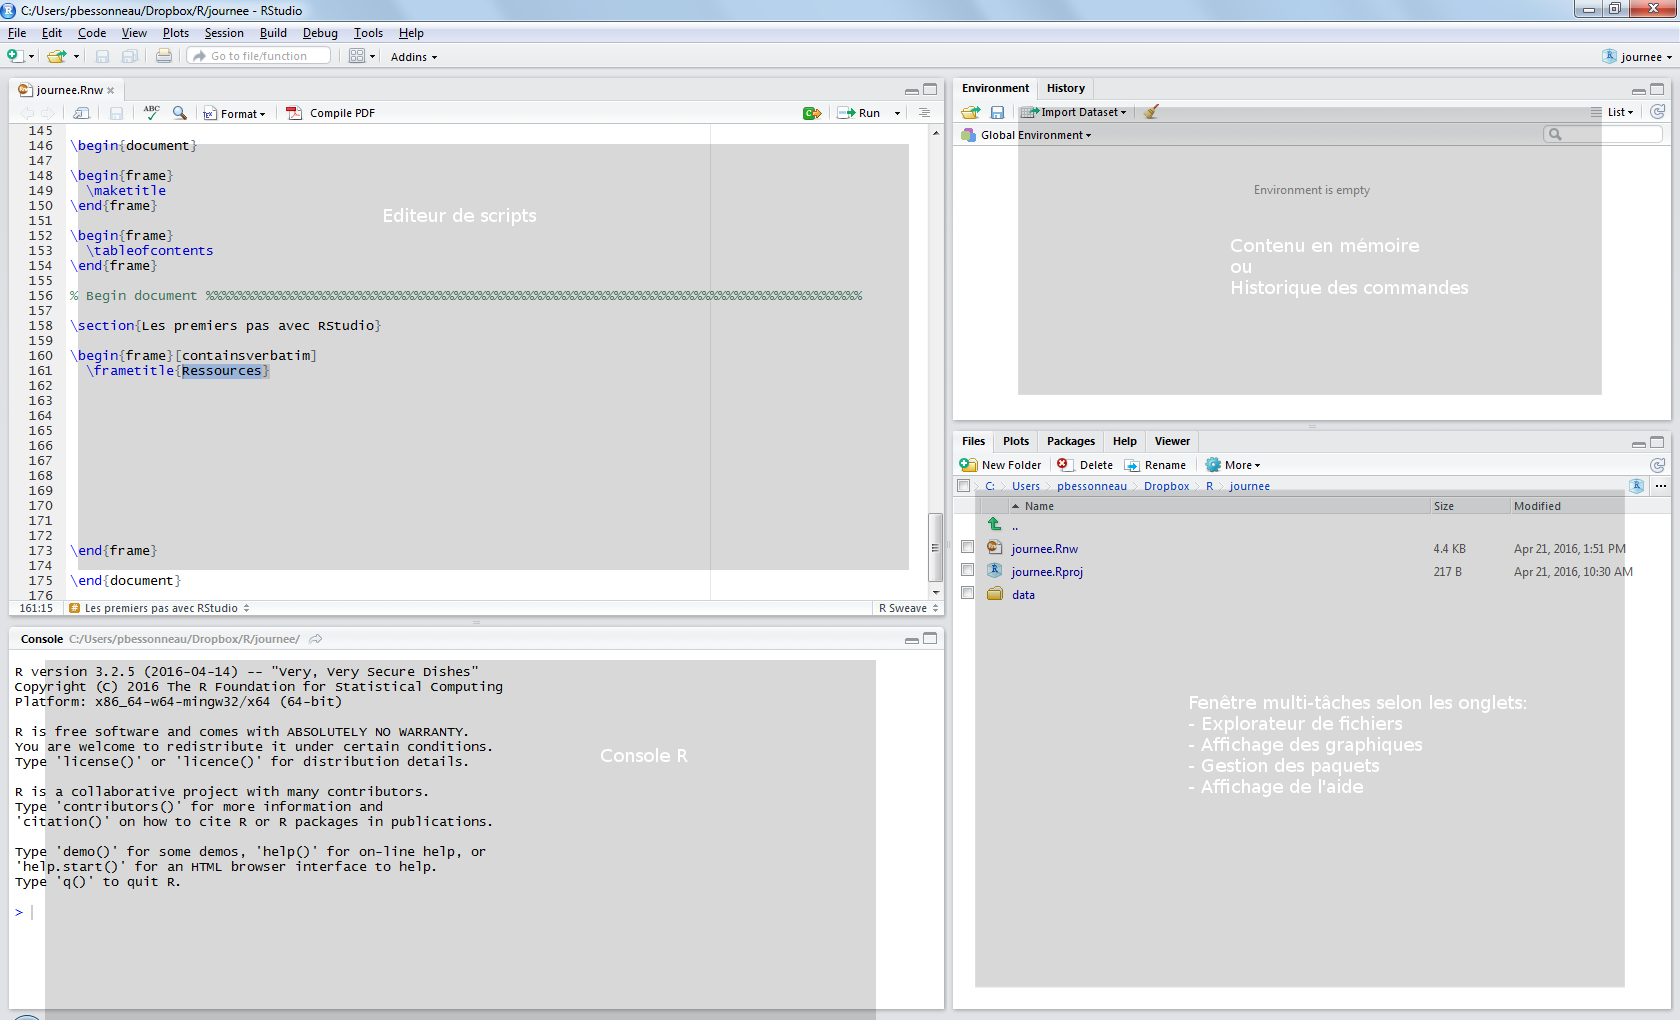
\includegraphics{graphiques/fenetres}
  }
  
\end{frame}


\begin{frame}[containsverbatim]
  \frametitle{Pr�sentation g�n�rale}
  
  Comme vous l'avez remarqu� dans chaque fen�tre, on passe d'une t�che � l'autre
  en utilisant 	\textbf{les onglets}~: par exemple pour passer de l'explorateur de 
  fichiers aux graphiques ou � l'aide (respectivement les onglets Files, 
  Plots et Help).
  
  Vous utiliserez essentiellement l'�diteur en haut � gauche.
  
  Nous donnons �galement les raccourcis-claviers car ils peuvent �tre tr�s pratiques.
  
\end{frame}

\begin{frame}[containsverbatim]
  \frametitle{Le fonctionnement}
  
  Tout en R est bas� sur la ligne de commande (historiquement R se pr�sente
  comme un shell).
  
  Dans RStudio vous tapez les commandes dans l'�diteur puis vous les soumettez
  � R en utilisant le bouton \emph{Run} en haut au milieu (ou en 
  utilisant CTRL+ENTREE).
  
  Par d�faut \emph{Run} ou CTRL+ENTREE soumettent la ligne sur laquelle se 
  trouve le curseur ou une s�lection du script.
  
\end{frame}

\begin{frame}[containsverbatim]
  \frametitle{Le fonctionnement}
  
  Quand vous cr�ez un graphique ou que vous demandez de l'aide alors l'onglet
  correspondant se met en avant tout seul en bas � droite.
  
  Dans R, tout est en m�moire vive (ou presque). En d�butant tout les objets
  que vous manipulez ou que vous cr�ez apparaissent dans la fen�tre en haut �
  droite~: c'est (presque) tout le contenu de la m�moire.
  
  Quand cet objet est une \emph{data.frame} vous pouvez cliquer pour 
  les visualiser (un peu comme dans un tableur). 
  
  Attention, m�me s'il est possible d'�diter ces donn�es c'est une op�ration � 
  proscrire.
  
\end{frame}

\section{Les diff�rentes fen�tres}

\begin{frame}[containsverbatim]
  \frametitle{L'�diteur (en haut � gauche)}
  
  Par d�faut l'�diteur est en mode \emph{Script R}. Par cons�quent il va 
  essayer d'interpr�ter le contenu de la fen�tre pour vous aider en vous 
  proposant les variables disponibles, les fonctions, etc.
  
  La compl�tion se fait avec la touche \emph{TAB}. 
  
\end{frame}

\begin{frame}[containsverbatim]
  \frametitle{L'�diteur (en haut � gauche)}
  
  \textcolor{red}{ATTENTION} comme il essaie d'interpr�ter ce que vous �crivez
  il peut ralentir voire boguer quand vous prenez des notes dans l'�diteur.
  
  Vous pouvez prendre des notes � condition de les mettre en commentaires. Pour
  cela commencer la ligne avec un \emph{\#}.
  
  Une solution facile est de taper vos notes, de s�lectionner le texte et de le
  mettre en commentaire en utilisant \emph{CTRL+SHIFT+C} (ou dans le menu 
  \emph{Code}). 
  
  Vous pouvez aussi cr�er et �diter des fichiers texte dans RStudio.
  
\end{frame}

\begin{frame}[containsverbatim]
  \frametitle{L'�diteur (en haut � gauche)}
  
  Les raccourcis-claviers les plus courants ~: 
  
  \begin{description}
    \item [CTRL+ENTREE] soumets la ligne ou la s�lection � la console R
    \item [CTRL+SHIFT+C] passer le contenu de script � commentaire ou l'inverse
    \item [CTRL+SHIFT+A] pour indenter le code s�lectionn� comme un pro
    \item [CTRL+1] rend active la fen�tre �diteur
    \item [CTRL+2] rend active la fen�tre console
  \end{description}
  
  Un cheatsheet est disponible sur le site de \href{http://www.rstudio.com/wp-content/uploads/2016/01/rstudio-IDE-cheatsheet.pdf}{RStudio}.

\end{frame}

\begin{frame}[containsverbatim]
  \frametitle{La fen�tre de l'environnement global (en haut � droite)}
  
  Vous trouverez dans la fen�tre de l'�vnirionnement globale la liste des objets 
  que vous avez cr��s ou charg�s en m�moire. Vous y trouvez ce qu'une commande 
  \emph{ls()} retourne.
  
  Si ce sont des \emph{data.frame} vous pouvez cliquer dessus pour ouvrir
  une vue "tableur". Seules les premi�res observations (et colonnes) sont visibles.
  
\end{frame}


\begin{frame}[containsverbatim]
  \frametitle{La console R}
  
  Vous pouvez y taper directement les commandes qui seront interpr�t�s par R. 
  
  Vous pouvez aussi voir dans cette fen�tre si il y a une erreur ou un message
  suite au code tap� ou au code soumis via l'�diteur. C'est dans cette fen�tre que vous retrouverez 
  l'�quivalent de la \emph{log} sous SAS.
  
  Vous avez acc�s � l'historique des commandes avec la fl�che \emph{en haut}.
  
\end{frame}

\begin{frame}[containsverbatim]
  \frametitle{La fen�tre multi-t�ches (en bas � droite)}
  
  Vous y trouvez l'aide, les graphiques, la gestion des paquets selon l'onglet
  que vous choisissez. A essayer~:
  
\begin{knitrout}\footnotesize
\definecolor{shadecolor}{rgb}{0.969, 0.969, 0.969}\color{fgcolor}\begin{kframe}
\begin{alltt}
\hlstd{> }\hlopt{?}\hlstd{rnorm}
\end{alltt}
\end{kframe}
\end{knitrout}
 
ou  
 
\begin{knitrout}\footnotesize
\definecolor{shadecolor}{rgb}{0.969, 0.969, 0.969}\color{fgcolor}\begin{kframe}
\begin{alltt}
\hlstd{> }\hlkwd{hist}\hlstd{(}\hlkwd{rnorm}\hlstd{(}\hlnum{1000}\hlstd{))}
\end{alltt}
\end{kframe}
\end{knitrout}
  
\end{frame}

\section{Les pas suivants\dots}

\begin{frame}[containsverbatim]
  \frametitle{Dans le futur}
  
  Apprenez � vous servir des projets\dots Ils permettent de travailler sur des projets
  diff�rents en conservant l'interface (fen�tre, contenu m�moire,\dots) exactement
  comme vous l'avez laiss� \emph{lors du dernier lancement de RStudio}.
  
  Outre la possibiit� de produire des documents \LaTeX, il est �galement possible de faire des documents
  HTML ou RTF incluant une belle pr�sentation et le code R � l'int�rieur\dots
  
  Pour ceux qui sont int�ress�s RStudio est un outil de choix pour Sweave/knitr,
  le d�veloppement de paquets, le suivi de version avec git (ou svn), etc.
  
\end{frame}

\end{document}

\section{Les types de donn�es}

  \subsection{Typage}
  
  En informatique, toutes les informations sont stock�es en binaire. 
  
  00111001 peut repr�senter aussi bien un nombre qu'un caract�re.
  
  Les types sont la nature des donn�es que l'on peut stocker.
  


  
  En R, il n'existe pas de typage fort, c'est-�-dire qu'une nouvelle variable
  est d�fini comme caract�re, num�rique en fonction de la premi�re valeur qu'on
  mets dedans (la plupart du temps). 
  
  De plus une variable peut changer de type simplement en rempla�ant le contenu
  par un autre. 
  
  Toutefois il existe des exceptions.
  

  \subsection{Les types de base}
  
  Les diff�rents types sont les suivants~:
  \begin{description}
    \item[integer] ou entier en fran�ais. Il permettent de sauvegarder des 
    nombres non d�cimaux
    \item[numeric] ce type sert � stocker des nombres d�cimaux
    \item[complex] ce type permet de stocker des nombres avec partie enti�re et 
    partie imaginaire des complexes
    \item[character] permet de stocker des chaines de caract�res
    \item[logical] permet de stocker des bool�ens (Vrai/Faux)
  \end{description}

    

    \begin{description}
      \item[les dates], comme souvent les dates sont des objets d�licats � 
      manipuler. Les termes qui font r�f�rence � des type diff�rents sont~:
      \emph{POSIXct},\emph{POSIXlt}, \dots
      \item[factor] les \emph{factor} ce sont des modalit�s de variable ordinale ou 
      qualitative      
      \item[AsIs] permet de stocker des donn�es en utilisant l'op�rateur 
      \emph{I()}. En pratique il se rencontre dans des fusions souvent c'est un 
      signe que vous devriez vous inqui�ter des r�sultats obtenus par la fusion

      \item[utilisateurs] des packages (ou vous m�me) vous pouvez cr�er des types
      nouveaux
  \end{description}
  

  \subsection{Les bool�ens}

  Les bool�ens sont des \emph{TRUE} ou \emph{FALSE} qui sont deux mots clefs
  de R. Ils peuvent �tre abr�g�s en \emph{T} ou \emph{F}.
  
  Les bool�ens peuvent convertis en num�riques naturellement ou explicitement.
  
  Dans ce cas leurs valeurs sont 0 pour FALSE et 1 pour TRUE. Ce qui autorise
  de faire des sommes de bool�en.
  


\section{Compl�ments sur les types de base}
  \subsection{Les \emph{factor}}

      Les \emph{factor} permettent de stocker des variables ayant peu de 
      modalit�s. C'est par exemple le cas pour stocker~: exp�rience A ou B, 
      m�dicament Placebo ou Actif. L'�tiquette est stock�e sous forme de texte 
      mais les facteurs sont aussi manipulables sous forme de nombres.
      
      Cette dualit� qui est tr�s utile dans un laboratoire pour faire des ANOVA
      est un vrai probl�me quand on stocke des donn�es complexes. 
      
      Si les facteurs sont indispensables pour faire certaines analyses comme
      les tests de Tukeyn certains auteurs font tout ( ou presque) pour �viter
      leur utilisation comme H. Wickham.
      

  

  \subsection{La pr�cision des nombres}
    
    Souvent, par exemple pour des entiers lors de sondages, il est n�cessaire
    de s'inqui�ter de la pr�cision des types num�riques. Ces limites peuvent
    d�pendre de la machine utilis�e.
    
    Ces informations sont contenues dans l'objet \emph{.Machine} que l'on peut
    taper directement ou on peut appeler seulement une partie.
    
    Par exemple pour trouver les entiers maximums que l'on peut stocker sur la
    machine qui a compil� ce document~:
    
\begin{knitrout}\footnotesize
\definecolor{shadecolor}{rgb}{0.969, 0.969, 0.969}\color{fgcolor}\begin{kframe}
\begin{alltt}
\hlstd{> }\hlstd{.Machine}\hlopt{$}\hlstd{integer.max}
\end{alltt}
\begin{verbatim}
## [1] 2147483647
\end{verbatim}
\end{kframe}
\end{knitrout}
    


\documentclass{beamer}\usepackage[]{graphicx}\usepackage[]{color}
%% maxwidth is the original width if it is less than linewidth
%% otherwise use linewidth (to make sure the graphics do not exceed the margin)
\makeatletter
\def\maxwidth{ %
  \ifdim\Gin@nat@width>\linewidth
    \linewidth
  \else
    \Gin@nat@width
  \fi
}
\makeatother

\definecolor{fgcolor}{rgb}{0.345, 0.345, 0.345}
\newcommand{\hlnum}[1]{\textcolor[rgb]{0.686,0.059,0.569}{#1}}%
\newcommand{\hlstr}[1]{\textcolor[rgb]{0.192,0.494,0.8}{#1}}%
\newcommand{\hlcom}[1]{\textcolor[rgb]{0.678,0.584,0.686}{\textit{#1}}}%
\newcommand{\hlopt}[1]{\textcolor[rgb]{0,0,0}{#1}}%
\newcommand{\hlstd}[1]{\textcolor[rgb]{0.345,0.345,0.345}{#1}}%
\newcommand{\hlkwa}[1]{\textcolor[rgb]{0.161,0.373,0.58}{\textbf{#1}}}%
\newcommand{\hlkwb}[1]{\textcolor[rgb]{0.69,0.353,0.396}{#1}}%
\newcommand{\hlkwc}[1]{\textcolor[rgb]{0.333,0.667,0.333}{#1}}%
\newcommand{\hlkwd}[1]{\textcolor[rgb]{0.737,0.353,0.396}{\textbf{#1}}}%

\usepackage{framed}
\makeatletter
\newenvironment{kframe}{%
 \def\at@end@of@kframe{}%
 \ifinner\ifhmode%
  \def\at@end@of@kframe{\end{minipage}}%
  \begin{minipage}{\columnwidth}%
 \fi\fi%
 \def\FrameCommand##1{\hskip\@totalleftmargin \hskip-\fboxsep
 \colorbox{shadecolor}{##1}\hskip-\fboxsep
     % There is no \\@totalrightmargin, so:
     \hskip-\linewidth \hskip-\@totalleftmargin \hskip\columnwidth}%
 \MakeFramed {\advance\hsize-\width
   \@totalleftmargin\z@ \linewidth\hsize
   \@setminipage}}%
 {\par\unskip\endMakeFramed%
 \at@end@of@kframe}
\makeatother

\definecolor{shadecolor}{rgb}{.97, .97, .97}
\definecolor{messagecolor}{rgb}{0, 0, 0}
\definecolor{warningcolor}{rgb}{1, 0, 1}
\definecolor{errorcolor}{rgb}{1, 0, 0}
\newenvironment{knitrout}{}{} % an empty environment to be redefined in TeX

\usepackage{alltt}
\usetheme[compress]{Singapore}
\useoutertheme{miniframes}

% \documentclass{beamer}
%\usetheme{Warsaw}

% Pour les documents en francais...
	\usepackage[latin1]{inputenc}
	\usepackage[french]{babel}
	\usepackage[french]{varioref}

% Math�matiques
	\usepackage{amsmath}

% Caracteres speciaux suppl�mentaires
	\usepackage{latexsym,amsfonts}

% A documenter
	\usepackage{moreverb}

% Macros pour les paquets
	\usepackage{array}  			% N�cessaires pour les tableaux de la macro Excel.

% Outil suppl�mentaire pour les tableaux
	\usepackage{multirow}
	\usepackage{booktabs}
	\usepackage{xcolor} % alternating row colors in table, incompatible avec certains modules
	\usepackage{longtable}
	\usepackage{colortbl}

% Pour ins�rer des graphiques
	\usepackage{graphicx} 			% Graphique simples
	\usepackage{subfigure}			% Graphiques multiples

% Pour ins�rer des couleurs
	\usepackage{color}

% Rotation des objets et des pages
%	\usepackage{rotating}
%	\usepackage{lscape}

% Pour insrer du code source, LaTeX ou SAS par exemple.
	\usepackage{verbatim}
        \usepackage{moreverb}
	\usepackage{listings}
	\usepackage{fancyvrb}

%	\lstset{language=SAS,numbers=left}		% Par dfaut le listing est en SAS

% Pour ins�rer des hyperliens
  \usepackage{hyperref}

% American Psychological Association (for bibliographic references).
	\usepackage{apacite}

% Pour l'utilisation des macros
	\usepackage{xspace}

% Pour l'utilisation de notes en fin de document.
%	\usepackage{endnotes}

% Array
%	\usepackage{multirow}
%	\usepackage{booktabs}

% Rotation
%	\usepackage{rotating}

% En t�tes et pieds de pages
%	\usepackage{fancyhdr}
%	\usepackage{lastpage}


% Page layout

% By LaTeX commands
%\setlength{\oddsidemargin}{0cm}
%\setlength{\textwidth}{16cm}
%\setlength{\textheight}{24cm}
%\setlength{\topmargin}{-1cm}
%\setlength{\marginparsep}{0.2cm}

% fancyheader parameters
%\pagestyle{fancy}

%\fancyfoot[L]{{\small Formation \LaTeX, DEPP}}
%\fancyfoot[c]{}
%\fancyfoot[R]{{\small \thepage/\pageref{LastPage}}}

%\fancyhead[L]{}
%\fancyhead[c]{}
%\fancyhead[R]{}

% Pour ins�rer des dessins de Linux
\newcommand{\LinuxA}{\includegraphics[height=0.5cm]{Graphiques/linux.png}}
\newcommand{\LinuxB}{\includegraphics[height=0.5cm]{Graphiques/linux.png}\xspace}

% Macro pour les petits dessins pour les diff�rents OS.
\newcommand{\Windows}{\emph{Windows}\xspace}
\newcommand{\Mac}{\emph{Mac OS X}\xspace}
\newcommand{\Linux}{\emph{Linux}\xspace}
\newcommand{\MikTeX}{MiK\tex\xspace}
\newcommand{\latex}{\LaTeX\xspace}


\newcommand{\df}{\emph{data.frame}\xspace}
\newcommand{\dfs}{\emph{data.frames}\xspace}
\newcommand{\liste}{\emph{list}\xspace}
\newcommand{\cad}{c'est-�-dire\xspace}

% Titre
\title{Introduction � R}
\author{Pascal Bessonneau}
%\institute{DEPP}
\date{06/2015}
\subtitle{Les types d'objets}


\newcommand{\hreff}[2]{\underline{\href{#1}{#2}\xspace}}



\IfFileExists{upquote.sty}{\usepackage{upquote}}{}
\begin{document}

\begin{frame}
	\maketitle
\end{frame}

\begin{frame}
	\tableofcontents
\end{frame}

% Begin document %%%%%%%%%%%%%%%%%%%%%%%%%%%%%%%%%%%%%%%%%%%%%%%%%%%%%%%%%%%%%%%


\section{les objets de base}

\begin{frame}[containsverbatim]
  \frametitle{Vecteurs}

  L'objet le plus courant est de loin le vecteur. il s'agit d'un tableau � 1 
  dimension stockant un seul et unique type de donn�es.
  
  La cr�ation d'un vecteur est soit implicite soit explicite.
  
  Implicite avec l'op�rateur \emph{c}~:
  
\begin{knitrout}\footnotesize
\definecolor{shadecolor}{rgb}{0.969, 0.969, 0.969}\color{fgcolor}\begin{kframe}
\begin{alltt}
\hlstd{> }\hlkwd{c}\hlstd{(}\hlnum{2}\hlstd{,}\hlnum{3}\hlstd{,}\hlnum{4}\hlstd{,}\hlnum{6}\hlstd{,}\hlnum{7}\hlstd{)}
\end{alltt}
\begin{verbatim}
## [1] 2 3 4 6 7
\end{verbatim}
\end{kframe}
\end{knitrout}

\end{frame}

\begin{frame}[containsverbatim]
  \frametitle{Vecteurs}

  Soit explicite en appelant un cr�ateur qui porte le nom du type que l'on 
  souhaite stock� et sa longueur~:
  
\begin{knitrout}\footnotesize
\definecolor{shadecolor}{rgb}{0.969, 0.969, 0.969}\color{fgcolor}\begin{kframe}
\begin{alltt}
\hlstd{> }\hlkwd{numeric}\hlstd{(}\hlnum{4}\hlstd{)}
\end{alltt}
\begin{verbatim}
## [1] 0 0 0 0
\end{verbatim}
\begin{alltt}
\hlstd{> }\hlkwd{logical}\hlstd{(}\hlnum{4}\hlstd{)}
\end{alltt}
\begin{verbatim}
## [1] FALSE FALSE FALSE FALSE
\end{verbatim}
\end{kframe}
\end{knitrout}

\end{frame}

\begin{frame}[containsverbatim]
  \frametitle{Les fonctions associ�es aux types}
  
  Il existe deux familles de fonctions associ�es aux types~:
  \begin{description}
    \item[is.] les fonctions \emph{is.} renvoie un bool�en indiquant si la valeur
    appartient � un type donn�
    \item[as.] ces fonctions permettent de changer le type d'une valeur vers une
    autre (cast)
  \end{description}
  
  
\begin{knitrout}\footnotesize
\definecolor{shadecolor}{rgb}{0.969, 0.969, 0.969}\color{fgcolor}\begin{kframe}
\begin{alltt}
\hlstd{> }\hlkwd{is.integer}\hlstd{(}\hlnum{2L}\hlstd{)}
\end{alltt}
\begin{verbatim}
## [1] TRUE
\end{verbatim}
\begin{alltt}
\hlstd{> }\hlkwd{is.character}\hlstd{(}\hlnum{2.3}\hlstd{)}
\end{alltt}
\begin{verbatim}
## [1] FALSE
\end{verbatim}
\begin{alltt}
\hlstd{> }\hlkwd{as.character}\hlstd{(}\hlnum{2}\hlstd{)}
\end{alltt}
\begin{verbatim}
## [1] "2"
\end{verbatim}
\end{kframe}
\end{knitrout}

\end{frame}

\begin{frame}[containsverbatim]
  \frametitle{Matrices}

  Ensuite viennent les matrices qui sont des tableaux � deux dimensions~:
  
\begin{knitrout}\footnotesize
\definecolor{shadecolor}{rgb}{0.969, 0.969, 0.969}\color{fgcolor}\begin{kframe}
\begin{alltt}
\hlstd{> }\hlkwd{matrix}\hlstd{(} \hlnum{0}\hlstd{,} \hlkwc{ncol} \hlstd{=} \hlnum{2}\hlstd{,} \hlkwc{nrow} \hlstd{=} \hlnum{2}\hlstd{)}
\end{alltt}
\begin{verbatim}
##      [,1] [,2]
## [1,]    0    0
## [2,]    0    0
\end{verbatim}
\end{kframe}
\end{knitrout}

  Les matrices sont cr��s avec un premier argument qui contient les donn�es et 
  une (ou deux tailles, largeur et/ou longueur).

\end{frame}

\begin{frame}[containsverbatim]
  \frametitle{Matrices}

  
\begin{knitrout}\footnotesize
\definecolor{shadecolor}{rgb}{0.969, 0.969, 0.969}\color{fgcolor}\begin{kframe}
\begin{alltt}
\hlstd{> }\hlkwd{matrix}\hlstd{(} \hlnum{0}\hlstd{,} \hlkwc{ncol} \hlstd{=} \hlnum{2}\hlstd{,} \hlkwc{nrow} \hlstd{=} \hlnum{2}\hlstd{)}
\end{alltt}
\begin{verbatim}
##      [,1] [,2]
## [1,]    0    0
## [2,]    0    0
\end{verbatim}
\end{kframe}
\end{knitrout}

  Les matrices sont cr��s avec un premier argument qui contient les donn�es et 
  une (ou deux tailles, largeur et/ou longueur).

  Le type de donn�es, \emph{unique}, stock� pour les matrices est le type de 
  donn�es par le premier argument.

\end{frame}

\begin{frame}[containsverbatim]
  \frametitle{les \emph{data.frame}}

  Les \dfs sont des tableaux comme les matrices mais qui permettent de stocker
  des types de donn�es diff�rentes dans chaque colonne.

\begin{knitrout}\footnotesize
\definecolor{shadecolor}{rgb}{0.969, 0.969, 0.969}\color{fgcolor}\begin{kframe}
\begin{alltt}
\hlstd{> }\hlkwd{head}\hlstd{(}\hlkwd{data.frame}\hlstd{(}\hlkwc{lettre}\hlstd{=LETTERS,}\hlkwc{numero}\hlstd{=}\hlnum{1}\hlopt{:}\hlnum{26}\hlstd{))}
\end{alltt}
\begin{verbatim}
##   lettre numero
## 1      A      1
## 2      B      2
## 3      C      3
## 4      D      4
## 5      E      5
## 6      F      6
\end{verbatim}
\end{kframe}
\end{knitrout}

\end{frame}

\begin{frame}[containsverbatim]
  \frametitle{les \emph{data.frame}}

  Les \dfs sont de loin la structure la plus utilis�e en faisant de la 
  manipulation de donn�es. 
  
  Mais ce type d�rive en fait d'un autre type de base moins manipulable par les
  d�butants~: les listes.

  
\end{frame}

\section{les objets moins courants}

\begin{frame}[containsverbatim]
  \frametitle{les \emph{list}}

  Les \emph{list} sont la structure la plus pratique. Ce sont des vecteurs o�
  chaque �lement du vecteur peut �tre un objet R quelconque y compris une liste.

\begin{knitrout}\footnotesize
\definecolor{shadecolor}{rgb}{0.969, 0.969, 0.969}\color{fgcolor}\begin{kframe}
\begin{alltt}
\hlstd{> }\hlstd{a}\hlkwb{=}\hlkwd{list}\hlstd{(}\hlnum{1}\hlstd{, LETTERS,} \hlkwd{matrix}\hlstd{(}\hlnum{0}\hlstd{,}\hlnum{2}\hlstd{,}\hlnum{2}\hlstd{))}
\hlstd{> }\hlkwd{str}\hlstd{(a)}
\end{alltt}
\begin{verbatim}
## List of 3
##  $ : num 1
##  $ : chr [1:26] "A" "B" "C" "D" ...
##  $ : num [1:2, 1:2] 0 0 0 0
\end{verbatim}
\end{kframe}
\end{knitrout}

\end{frame}


\begin{frame}[containsverbatim]
  \frametitle{les \emph{list}}

  Les \dfs sont en fait une liste avec comme condition que chaque �lement soit
  un vecteur de m�me longueur (pour obtenir un tableau).
  
  Ainsi les listes et les \dfs partagent beaucoup d'op�rateurs en communs.

\end{frame}

\begin{frame}[containsverbatim]
  \frametitle{les \emph{array}}

  les \emph{array} sont des objets qui �tendent les matrices � des tableaux
  � \emph{k}-dimsions. 
  
\begin{knitrout}\footnotesize
\definecolor{shadecolor}{rgb}{0.969, 0.969, 0.969}\color{fgcolor}\begin{kframe}
\begin{alltt}
\hlstd{> }\hlkwd{array}\hlstd{(}\hlnum{1}\hlopt{:}\hlnum{4}\hlstd{,}\hlkwd{c}\hlstd{(}\hlnum{2}\hlstd{,}\hlnum{2}\hlstd{,}\hlnum{2}\hlstd{))}
\end{alltt}
\begin{verbatim}
## , , 1
## 
##      [,1] [,2]
## [1,]    1    3
## [2,]    2    4
## 
## , , 2
## 
##      [,1] [,2]
## [1,]    1    3
## [2,]    2    4
\end{verbatim}
\end{kframe}
\end{knitrout}

\end{frame}

\begin{frame}[containsverbatim]
  \frametitle{les \emph{list}}

  Les \dfs sont en fait une liste avec comme condition que chaque �lement soit
  un vecteur de m�me longueur (pour obtenir un tableau).
  
  Ainsi les listes et les \dfs partagent beaucoup d'op�rateurs en communs.

  Dans la programmation avanc�e, les \dfs sont souvent utilis�es comme des 
  listes.

\end{frame}

\begin{frame}[containsverbatim]
  \frametitle{les s�ries temporelles}

  Les s�ries temporelles sont des des �lements pouvant stocker et avec des 
  propri�t�s particuli�res des s�ries de date.
  
  C'est le type utilis� pour tous les analyses en s�ries temporelles.
  
\begin{knitrout}\footnotesize
\definecolor{shadecolor}{rgb}{0.969, 0.969, 0.969}\color{fgcolor}\begin{kframe}
\begin{alltt}
\hlstd{> }\hlkwd{ts}\hlstd{(}\hlkwd{date}\hlstd{())}
\end{alltt}
\begin{verbatim}
## Time Series:
## Start = 1 
## End = 1 
## Frequency = 1 
## [1] Sat May 21 04:29:45 2016
\end{verbatim}
\end{kframe}
\end{knitrout}
  
\end{frame}

\begin{frame}[containsverbatim]
  \frametitle{Les fonctions de transformation}
  
  Il existe deux familles de fonctions associ�es aux types~:
  \begin{description}
    \item[is.] les fonctions \emph{is.} renvoie un bool�en indiquant si la valeur
    appartient � un objet donn�
    \item[as.] ces fonctions permettent de changer un objet dans un autre type
  \end{description}

\begin{knitrout}\footnotesize
\definecolor{shadecolor}{rgb}{0.969, 0.969, 0.969}\color{fgcolor}\begin{kframe}
\begin{alltt}
\hlstd{> }\hlkwd{str}\hlstd{(}\hlkwd{as.list}\hlstd{(iris))}
\end{alltt}
\begin{verbatim}
## List of 5
##  $ Sepal.Length: num [1:150] 5.1 4.9 4.7 4.6 5 5.4 4.6 5 4.4 4.9 ...
##  $ Sepal.Width : num [1:150] 3.5 3 3.2 3.1 3.6 3.9 3.4 3.4 2.9 3.1 ...
##  $ Petal.Length: num [1:150] 1.4 1.4 1.3 1.5 1.4 1.7 1.4 1.5 1.4 1.5 ...
##  $ Petal.Width : num [1:150] 0.2 0.2 0.2 0.2 0.2 0.4 0.3 0.2 0.2 0.1 ...
##  $ Species     : Factor w/ 3 levels "setosa","versicolor",..: 1 1 1 1 1 1 1 1 1 1 ...
\end{verbatim}
\begin{alltt}
\hlstd{> }\hlkwd{str}\hlstd{(}\hlkwd{as.matrix}\hlstd{(iris[,}\hlnum{1}\hlopt{:}\hlnum{4}\hlstd{]))}
\end{alltt}
\begin{verbatim}
##  num [1:150, 1:4] 5.1 4.9 4.7 4.6 5 5.4 4.6 5 4.4 4.9 ...
##  - attr(*, "dimnames")=List of 2
##   ..$ : NULL
##   ..$ : chr [1:4] "Sepal.Length" "Sepal.Width" "Petal.Length" "Petal.Width"
\end{verbatim}
\end{kframe}
\end{knitrout}

\end{frame}

\section{Nommage des �lements d'un objet}

% � remplir


\section{Les trois aspects de l'indexation}

\begin{frame}[containsverbatim]
  \frametitle{Dans cette partie\dots}
  
  \dots sont d�crites les principales r�gles qui permettent de s�lectionner une
  partie des objets les plus courants (le langage objet S4 est exclus).
  
\end{frame}

\begin{frame}[containsverbatim]
  \frametitle{Pour un vecteur}

    Pour un vecteur, l'op�rateur d'extraction de valeurs sont des crochets.
    simples.
    
    Comme on peut le voir sur les deux derni�res lignes leur pr�c�dence n'est pas
    tr�s forte mais plus grande que les op�rateurs de calcul.
    
\begin{knitrout}\footnotesize
\definecolor{shadecolor}{rgb}{0.969, 0.969, 0.969}\color{fgcolor}\begin{kframe}
\begin{alltt}
\hlstd{> }\hlstd{LETTERS[}\hlnum{1}\hlopt{:}\hlnum{10}\hlstd{]}
\end{alltt}
\begin{verbatim}
##  [1] "A" "B" "C" "D" "E" "F" "G" "H" "I" "J"
\end{verbatim}
\begin{alltt}
\hlstd{> }\hlkwd{c}\hlstd{(}\hlnum{1}\hlstd{,}\hlnum{2}\hlstd{,}\hlnum{3}\hlstd{,}\hlnum{4}\hlstd{)[}\hlnum{1}\hlopt{:}\hlnum{2}\hlstd{]}
\end{alltt}
\begin{verbatim}
## [1] 1 2
\end{verbatim}
\begin{alltt}
\hlstd{> }\hlkwd{c}\hlstd{(}\hlnum{1}\hlstd{,}\hlnum{2}\hlstd{,}\hlnum{3}\hlstd{,}\hlnum{4}\hlstd{)[}\hlopt{-}\hlnum{4}\hlstd{]}
\end{alltt}
\begin{verbatim}
## [1] 1 2 3
\end{verbatim}
\begin{alltt}
\hlstd{> }\hlkwd{c}\hlstd{(}\hlnum{1}\hlstd{,}\hlnum{2}\hlstd{,}\hlnum{3}\hlstd{,}\hlnum{4}\hlstd{)[}\hlopt{-}\hlnum{4}\hlstd{]} \hlopt{*} \hlnum{2}
\end{alltt}
\begin{verbatim}
## [1] 2 4 6
\end{verbatim}
\end{kframe}
\end{knitrout}

\end{frame}


\begin{frame}[containsverbatim]
  \frametitle{Les trois aspects de l'indexation}

    L'indexation sauf certaine exception peut se faire avec trois types de 
    donn�es sous R.
    \begin{description}
      \item[entiers] avec les entiers, les chiffres positifs indiquent les
      positions des vecteurs qui seront extraits. Les chiffres n�gatifs indiquent
      les positions � exclure. Attention on ne peux pas m�langer chiffre
      positif et chiffres n�gatifs
    \end{description}
    
\end{frame}
    
\begin{frame}[containsverbatim]
  \frametitle{les entiers}

  Avec les entiers, les chiffres positifs indiquent les positions des vecteurs 
  qui seront extraits. Les chiffres n�gatifs indiquent les positions � exclure. 
  
  La longueur est quelconque (mais sup�rieur ou �gal � 1). La longueur 
  corresponds au nombre de d'�l�ments � extraire (ou � ne pas extraire).
  
  Attention on ne peux pas m�langer chiffres positifs et chiffres n�gatifs
  
  Attention Attention, amoureux du C et du perl, le z�ro n'est jamais un indice 
  valide en R.
  
\end{frame}

\begin{frame}[containsverbatim]
  \frametitle{les entiers}
  
  
  La longueur du vecteur retourn� est la longueur du vecteur de s�lection pour
  les nombres d'entiers. 
  
  Pour les nombres n�gatifs, la longueur retourn�e est le total d'elements uniques
  du vecteurs moins la longueur du vecteur de s�lection.
  
\end{frame}

\begin{frame}[containsverbatim]
  \frametitle{les entiers}
  
\begin{knitrout}\footnotesize
\definecolor{shadecolor}{rgb}{0.969, 0.969, 0.969}\color{fgcolor}\begin{kframe}
\begin{alltt}
\hlstd{> }\hlstd{LETTERS[}\hlkwd{c}\hlstd{(}\hlnum{1}\hlstd{,}\hlnum{2}\hlstd{,}\hlnum{3}\hlstd{,}\hlnum{4}\hlstd{)]}
\end{alltt}
\begin{verbatim}
## [1] "A" "B" "C" "D"
\end{verbatim}
\begin{alltt}
\hlstd{> }\hlstd{LETTERS[}\hlkwd{c}\hlstd{(}\hlnum{2}\hlstd{,}\hlnum{4}\hlstd{)]}
\end{alltt}
\begin{verbatim}
## [1] "B" "D"
\end{verbatim}
\begin{alltt}
\hlstd{> }\hlstd{LETTERS[}\hlkwd{c}\hlstd{(}\hlnum{2}\hlstd{,}\hlnum{4}\hlstd{,}\hlnum{2}\hlstd{)]}
\end{alltt}
\begin{verbatim}
## [1] "B" "D" "B"
\end{verbatim}
\end{kframe}
\end{knitrout}

\end{frame}

\begin{frame}[containsverbatim]
  \frametitle{les entiers}
  
\begin{knitrout}\footnotesize
\definecolor{shadecolor}{rgb}{0.969, 0.969, 0.969}\color{fgcolor}\begin{kframe}
\begin{alltt}
\hlstd{> }\hlstd{LETTERS[}\hlopt{-}\hlkwd{c}\hlstd{(}\hlnum{1}\hlstd{,}\hlnum{2}\hlstd{,}\hlnum{3}\hlstd{,}\hlnum{4}\hlstd{)]}
\end{alltt}
\begin{verbatim}
##  [1] "E" "F" "G" "H" "I" "J" "K" "L" "M" "N"
## [11] "O" "P" "Q" "R" "S" "T" "U" "V" "W" "X"
## [21] "Y" "Z"
\end{verbatim}
\begin{alltt}
\hlstd{> }\hlstd{LETTERS[}\hlopt{-}\hlkwd{c}\hlstd{(}\hlnum{2}\hlstd{,}\hlnum{4}\hlstd{)]}
\end{alltt}
\begin{verbatim}
##  [1] "A" "C" "E" "F" "G" "H" "I" "J" "K" "L"
## [11] "M" "N" "O" "P" "Q" "R" "S" "T" "U" "V"
## [21] "W" "X" "Y" "Z"
\end{verbatim}
\begin{alltt}
\hlstd{> }\hlstd{LETTERS[}\hlopt{-}\hlkwd{c}\hlstd{(}\hlnum{2}\hlstd{,}\hlnum{4}\hlstd{,}\hlnum{2}\hlstd{)]}
\end{alltt}
\begin{verbatim}
##  [1] "A" "C" "E" "F" "G" "H" "I" "J" "K" "L"
## [11] "M" "N" "O" "P" "Q" "R" "S" "T" "U" "V"
## [21] "W" "X" "Y" "Z"
\end{verbatim}
\end{kframe}
\end{knitrout}
  
\end{frame}


\begin{frame}[containsverbatim]
  \frametitle{le vecteur logique}
  
  La grande diff�rence avec les indices num�riques est la longueur du vecteur.
  
  Pour chaque position, si la valeur est \emph{TRUE}, la valeur est retourn�e.
  Si c'est \emph{FALSE}, la valeur n'est pas retourn�.
  
  Par cons�quent la longueur du vecteur de s�lection est la longueur du vecteur
  � s�l�ctionner. Quant � la la longueur du vecteur de retour, c'est le nombre
  de \emph{TRUE} (ie. la somme du vecteur logique).
  
  Attention au recyclage ! Si le recyclage n'est pas possible R g�n�re une erreur
  si la longueur des deux vecteurs ne co�ncide pas.
  
\end{frame}

\begin{frame}[containsverbatim]
  \frametitle{le vecteur logique}

\begin{knitrout}\footnotesize
\definecolor{shadecolor}{rgb}{0.969, 0.969, 0.969}\color{fgcolor}\begin{kframe}
\begin{alltt}
\hlstd{> }\hlstd{L} \hlkwb{<-} \hlstd{LETTERS[}\hlnum{1}\hlopt{:}\hlnum{6}\hlstd{]}
\hlstd{> }\hlstd{L}
\end{alltt}
\begin{verbatim}
## [1] "A" "B" "C" "D" "E" "F"
\end{verbatim}
\begin{alltt}
\hlstd{> }\hlstd{L[}\hlkwd{c}\hlstd{(T,F,T,F,T,T)]}
\end{alltt}
\begin{verbatim}
## [1] "A" "C" "E" "F"
\end{verbatim}
\begin{alltt}
\hlstd{> }\hlstd{L[}\hlkwd{c}\hlstd{(T,F)]} \hlcom{# recyclage}
\end{alltt}
\begin{verbatim}
## [1] "A" "C" "E"
\end{verbatim}
\end{kframe}
\end{knitrout}

\end{frame}

\begin{frame}[containsverbatim]
  \frametitle{les noms}

  Les noms ont �t� �voqu�s bri�vement\dots � peu pr�s tout sous R peut porter un
  noms. 
  
  On peut donc utiliser un vecteur \emph{character} avec le noms des �lements
  pour les r�cup�rer.

  Les noms peuvent �tre utilis�s en lieu et place des num�ros. La longueur du
  vecteur de retour est alors le nombre de noms mis en arguments.
  
\end{frame}

\begin{frame}[containsverbatim]
  \frametitle{les noms}

\begin{knitrout}\footnotesize
\definecolor{shadecolor}{rgb}{0.969, 0.969, 0.969}\color{fgcolor}\begin{kframe}
\begin{alltt}
\hlstd{> }\hlstd{(a} \hlkwb{<-} \hlnum{1}\hlopt{:}\hlnum{4}\hlstd{)}
\end{alltt}
\begin{verbatim}
## [1] 1 2 3 4
\end{verbatim}
\begin{alltt}
\hlstd{> }\hlstd{(}\hlkwd{names}\hlstd{(a)} \hlkwb{<-} \hlstd{LETTERS[}\hlnum{1}\hlopt{:}\hlnum{4}\hlstd{])}
\end{alltt}
\begin{verbatim}
## [1] "A" "B" "C" "D"
\end{verbatim}
\begin{alltt}
\hlstd{> }\hlstd{a[}\hlkwd{c}\hlstd{(}\hlstr{"A"}\hlstd{,}\hlstr{"D"}\hlstd{,}\hlstr{"A"}\hlstd{,}\hlstr{"C"}\hlstd{)]}
\end{alltt}
\begin{verbatim}
## A D A C 
## 1 4 1 3
\end{verbatim}
\end{kframe}
\end{knitrout}

\end{frame}

\begin{frame}[containsverbatim]
  \frametitle{G�n�ralisation du syst�me d'indexation}
  
  Une fois compris ce syst�me d'indexation, le plus dur est   fait car c'est sur
  ce syst�me que se base pratiquement tout l'indexation des lignes et des
  colonnes d'une matrice, des �lements d'une liste, \dots
  
  Quand l'objet est compos� de lignes et de colonnes il suffit d'indexer et 
  d'ajouter une "," pour indiquer � R sur quel dimensions on travaille.
  
\end{frame}

\begin{frame}[containsverbatim]
  \frametitle{\dfs et matrices}
  
\begin{knitrout}\footnotesize
\definecolor{shadecolor}{rgb}{0.969, 0.969, 0.969}\color{fgcolor}\begin{kframe}
\begin{alltt}
\hlstd{> }\hlkwd{str}\hlstd{(iris[}\hlkwd{c}\hlstd{(}\hlnum{1}\hlstd{,}\hlnum{3}\hlstd{,}\hlnum{4}\hlstd{),])} \hlcom{# � gauche -> lignes}
\end{alltt}
\begin{verbatim}
## 'data.frame':	3 obs. of  5 variables:
##  $ Sepal.Length: num  5.1 4.7 4.6
##  $ Sepal.Width : num  3.5 3.2 3.1
##  $ Petal.Length: num  1.4 1.3 1.5
##  $ Petal.Width : num  0.2 0.2 0.2
##  $ Species     : Factor w/ 3 levels "setosa","versicolor",..: 1 1 1
\end{verbatim}
\begin{alltt}
\hlstd{> }\hlkwd{str}\hlstd{(iris[,}\hlkwd{c}\hlstd{(}\hlnum{2}\hlstd{,}\hlnum{4}\hlstd{,}\hlnum{5}\hlstd{)])} \hlcom{# � doirte -> colonnes}
\end{alltt}
\begin{verbatim}
## 'data.frame':	150 obs. of  3 variables:
##  $ Sepal.Width: num  3.5 3 3.2 3.1 3.6 3.9 3.4 3.4 2.9 3.1 ...
##  $ Petal.Width: num  0.2 0.2 0.2 0.2 0.2 0.4 0.3 0.2 0.2 0.1 ...
##  $ Species    : Factor w/ 3 levels "setosa","versicolor",..: 1 1 1 1 1 1 1 1 1 1 ...
\end{verbatim}
\begin{alltt}
\hlstd{> }\hlkwd{str}\hlstd{(iris[}\hlkwd{c}\hlstd{(}\hlnum{2}\hlstd{,}\hlnum{4}\hlstd{,}\hlnum{5}\hlstd{),}\hlkwd{c}\hlstd{(}\hlnum{2}\hlstd{,}\hlnum{4}\hlstd{,}\hlnum{5}\hlstd{)])} \hlcom{# les deux}
\end{alltt}
\begin{verbatim}
## 'data.frame':	3 obs. of  3 variables:
##  $ Sepal.Width: num  3 3.1 3.6
##  $ Petal.Width: num  0.2 0.2 0.2
##  $ Species    : Factor w/ 3 levels "setosa","versicolor",..: 1 1 1
\end{verbatim}
\end{kframe}
\end{knitrout}

\end{frame}


\begin{frame}[containsverbatim]
  \frametitle{Listes}
  
  Les listes sont proches des vecteurs. Les m�mes r�gles peuvent �tre appliqu�es.
  
  Il y a toutefois une subtilit�. Entre crochets simples, les listes renvoie
  une liste. Mais entre crochets doubles, un seul �lement peut �tre renvoy� mais
  l'�lement n'est pas de type liste mais du type contenu dans la liste � cette 
  position.
  
  C'est logique puisque vu l'h�t�rog�n�it� des �lements pouvant �tre stock�s
  dans une liste, R ne peut d�terminer la meilleure strat�gie pour rendre une
  s�rie d'objets h�t�rog�ne.
  
  Par contre quand un seul objet est renvoy� ce probl�me ne se pose pas.
  
\end{frame}

\begin{frame}[containsverbatim]
  \frametitle{Listes}

\begin{knitrout}\footnotesize
\definecolor{shadecolor}{rgb}{0.969, 0.969, 0.969}\color{fgcolor}\begin{kframe}
\begin{alltt}
\hlstd{> }\hlstd{a} \hlkwb{<-} \hlkwd{list}\hlstd{(}\hlnum{1}\hlstd{, LETTERS,} \hlkwd{matrix}\hlstd{(}\hlnum{0}\hlstd{,}\hlnum{2}\hlstd{,}\hlnum{2}\hlstd{))}
\hlstd{> }\hlstd{a[}\hlkwd{c}\hlstd{(T,F,T)]}
\end{alltt}
\begin{verbatim}
## [[1]]
## [1] 1
## 
## [[2]]
##      [,1] [,2]
## [1,]    0    0
## [2,]    0    0
\end{verbatim}
\begin{alltt}
\hlstd{> }\hlstd{a[[}\hlnum{1}\hlstd{]]}
\end{alltt}
\begin{verbatim}
## [1] 1
\end{verbatim}
\end{kframe}
\end{knitrout}

\end{frame}

\end{document}

\section{Les iris de Fisher}

  \subsection{Les iris de Fisher}

  Les iris de Fisher sont des donn�es tr�s connues dans le milieu des statisticiens.
  
  Ils consituent un jeu de donn�es sur lesquelles on utilise des m�thodes de 
  classification notamment.
  
  Ce sont les caract�ristiques morphologiques des feuilles pour quelques esp�ces
  d'Iris.
  



  
\begin{knitrout}\footnotesize
\definecolor{shadecolor}{rgb}{0.969, 0.969, 0.969}\color{fgcolor}\begin{kframe}
\begin{alltt}
\hlstd{> }\hlkwd{data}\hlstd{(iris)}
\hlstd{> }\hlkwd{class}\hlstd{(iris)}
\end{alltt}
\begin{verbatim}
## [1] "data.frame"
\end{verbatim}
\end{kframe}
\end{knitrout}




\begin{knitrout}\footnotesize
\definecolor{shadecolor}{rgb}{0.969, 0.969, 0.969}\color{fgcolor}\begin{kframe}
\begin{alltt}
\hlstd{> }\hlkwd{summary}\hlstd{(iris)}
\end{alltt}
\begin{verbatim}
##   Sepal.Length    Sepal.Width   
##  Min.   :4.300   Min.   :2.000  
##  1st Qu.:5.100   1st Qu.:2.800  
##  Median :5.800   Median :3.000  
##  Mean   :5.843   Mean   :3.057  
##  3rd Qu.:6.400   3rd Qu.:3.300  
##  Max.   :7.900   Max.   :4.400  
##   Petal.Length    Petal.Width   
##  Min.   :1.000   Min.   :0.100  
##  1st Qu.:1.600   1st Qu.:0.300  
##  Median :4.350   Median :1.300  
##  Mean   :3.758   Mean   :1.199  
##  3rd Qu.:5.100   3rd Qu.:1.800  
##  Max.   :6.900   Max.   :2.500  
##        Species  
##  setosa    :50  
##  versicolor:50  
##  virginica :50  
##                 
##                 
## 
\end{verbatim}
\end{kframe}
\end{knitrout}



\begin{knitrout}\footnotesize
\definecolor{shadecolor}{rgb}{0.969, 0.969, 0.969}\color{fgcolor}\begin{kframe}
\begin{alltt}
\hlstd{> }\hlkwd{table}\hlstd{(iris}\hlopt{$}\hlstd{Species)}
\end{alltt}
\begin{verbatim}
## 
##     setosa versicolor  virginica 
##         50         50         50
\end{verbatim}
\begin{alltt}
\hlstd{> }\hlkwd{prop.table}\hlstd{(}\hlkwd{table}\hlstd{(iris}\hlopt{$}\hlstd{Species))}
\end{alltt}
\begin{verbatim}
## 
##     setosa versicolor  virginica 
##  0.3333333  0.3333333  0.3333333
\end{verbatim}
\begin{alltt}
\hlstd{> }\hlkwd{prop.table}\hlstd{(}\hlkwd{table}\hlstd{(iris}\hlopt{$}\hlstd{Species))}\hlopt{*}\hlnum{100}
\end{alltt}
\begin{verbatim}
## 
##     setosa versicolor  virginica 
##   33.33333   33.33333   33.33333
\end{verbatim}
\end{kframe}
\end{knitrout}




\begin{knitrout}\footnotesize
\definecolor{shadecolor}{rgb}{0.969, 0.969, 0.969}\color{fgcolor}\begin{kframe}
\begin{alltt}
\hlstd{> }\hlkwd{tapply}\hlstd{(iris}\hlopt{$}\hlstd{Sepal.Length,iris}\hlopt{$}\hlstd{Species,mean)}
\end{alltt}
\begin{verbatim}
##     setosa versicolor  virginica 
##      5.006      5.936      6.588
\end{verbatim}
\end{kframe}
\end{knitrout}


\section{Les pr�noms}

  \subsection{Les pr�noms � Paris}

  Ce sont les pr�noms des nouveaux n�s � Paris. Ils viennent de 
  \href{http://opendata.paris.fr/explore/dataset/liste_des_prenoms_2004_a_2012/information/?disjunctive.prenoms&disjunctive.annee}{opendata.paris.fr}.
  
  Le but ici est de manipuler et d'extraire les donn�es. 
  


Pour charger le fichier~:

\begin{knitrout}\footnotesize
\definecolor{shadecolor}{rgb}{0.969, 0.969, 0.969}\color{fgcolor}\begin{kframe}
\begin{alltt}
\hlstd{> }\hlstd{prenoms} \hlkwb{<-} \hlkwd{read.csv2}\hlstd{(}\hlstr{"data/prenoms/liste_des_prenoms_2004_a_2012.csv"}\hlstd{,}
\hlstd{+ }                     \hlkwc{stringsAsFactors} \hlstd{= F,}\hlkwc{encoding} \hlstd{=} \hlstr{"UTF-8"}\hlstd{)}
\hlstd{> }\hlstd{p} \hlkwb{<-} \hlkwd{fromJSON}\hlstd{(}\hlstr{"data/prenoms/liste_des_prenoms_2004_a_2012.json"}\hlstd{)}\hlopt{$}\hlstd{fields}
\hlstd{> }
\hlstd{> }\hlkwd{colnames}\hlstd{(prenoms)}
\end{alltt}
\begin{verbatim}
## [1] "Prenoms" "Nombre"  "Sexe"    "Annee"
\end{verbatim}
\end{kframe}
\end{knitrout}
  


Pour r�cup�rer les pr�noms de 2004~:

\begin{knitrout}\footnotesize
\definecolor{shadecolor}{rgb}{0.969, 0.969, 0.969}\color{fgcolor}\begin{kframe}
\begin{alltt}
\hlstd{> }\hlstd{prenoms2004} \hlkwb{<-} \hlstd{prenoms[prenoms}\hlopt{$}\hlstd{Annee}\hlopt{==}\hlnum{2004}\hlstd{,]}
\end{alltt}
\end{kframe}
\end{knitrout}
  




Quel est le pr�nom le plus fr�quent ?

\begin{knitrout}\footnotesize
\definecolor{shadecolor}{rgb}{0.969, 0.969, 0.969}\color{fgcolor}\begin{kframe}
\begin{alltt}
\hlstd{> }\hlkwd{max}\hlstd{(prenoms}\hlopt{$}\hlstd{Nombre)}
\end{alltt}
\begin{verbatim}
## [1] 398
\end{verbatim}
\begin{alltt}
\hlstd{> }\hlstd{prenoms2004}\hlopt{$}\hlstd{Prenoms[prenoms2004}\hlopt{$}\hlstd{Nombre} \hlopt{==} \hlkwd{max}\hlstd{(prenoms2004}\hlopt{$}\hlstd{Nombre)]}
\end{alltt}
\begin{verbatim}
## [1] "Alexandre"
\end{verbatim}
\end{kframe}
\end{knitrout}
  


Quel est le pr�nom le moins fr�quent ?

\begin{knitrout}\footnotesize
\definecolor{shadecolor}{rgb}{0.969, 0.969, 0.969}\color{fgcolor}\begin{kframe}
\begin{alltt}
\hlstd{> }\hlstd{prenoms2004}\hlopt{$}\hlstd{Prenoms[prenoms2004}\hlopt{$}\hlstd{Nombre} \hlopt{==} \hlkwd{min}\hlstd{(prenoms2004}\hlopt{$}\hlstd{Nombre)]}
\end{alltt}
\end{kframe}
\end{knitrout}

\begin{knitrout}\footnotesize
\definecolor{shadecolor}{rgb}{0.969, 0.969, 0.969}\color{fgcolor}\begin{kframe}
\begin{verbatim}
##   [1] "Khalil"     "Leana"      "Loubna"    
##   [4] "Morgan"     "Natalia"    "Oussama"   
##   [7] "Safa"       "Sharon"     "Solenn"    
##  [10] "Sylvia"     "Viktor"     "Virgil"    
##  [13] "Wandrille"  "Warren"     "Alexane"   
##  [16] NA           "Camelia"    "Carl"      
##  [19] "Chanel"     "Filipe"     "Halima"    
##  [22] "Henry"      "Iban"       "Jawad"     
##  [25] "Josh"       "Adil"       "Bahia"     
##  [28] "Boubou"     "Clothilde"  "Dana"      
##  [31] "Daria"      "Gabriella"  "Harold"    
##  [34] "Hasna"      NA           "Latifa"    
##  [37] "Louka"      "Mory"       "Nesrine"   
##  [40] "Niouma"     "Rami"       "Ramy"      
##  [43] "Reda"       "Sebastian"  "Tim"       
##  [46] "Wendy"      NA           "Aboubakar" 
##  [49] "Adeline"    "Aymane"     "Benoit"    
##  [52] "Betty"      "Brune"      NA          
##  [55] "Colette"    "Cyriaque"   "Djeneba"   
##  [58] "Doriane"    "Elio"       "Germain"   
##  [61] "Guy"        "Ian"        "Idris"     
##  [64] "Ilyass"     "Khady"      "Nayla"     
##  [67] "Patricia"   "Sadio"      "Sylvain"   
##  [70] "Vladimir"   "Yanni"      "Khadija"   
##  [73] "Lamine"     "Lirone"     "Liza"      
##  [76] "Manuel"     "Naya"       "Nikita"    
##  [79] "Olympe"     "Perle"      "Solveig"   
##  [82] "Terence"    "Wilfried"   "Yossef"    
##  [85] NA           "Albert"     "Alissa"    
##  [88] "Aris"       "Calvin"     "Abdellah"  
##  [91] "Amara"      "Harry"      "Amelia"    
##  [94] "Athena"     "Brayan"     "Chelsea"   
##  [97] "Elena"      "Eliane"     "Elya"      
## [100] "Emy"        "Florence"   "Gad"       
## [103] NA           "Joey"       "Kadidiatou"
## [106] "Luce"       "Mahe"       "Meline"    
## [109] "Nael"       "Odelia"     "Oren"      
## [112] "Paco"       "Satine"     "Tao"       
## [115] NA
\end{verbatim}
\end{kframe}
\end{knitrout}
  



Quel est le minimum ?
\begin{knitrout}\footnotesize
\definecolor{shadecolor}{rgb}{0.969, 0.969, 0.969}\color{fgcolor}\begin{kframe}
\begin{alltt}
\hlstd{> }\hlkwd{min}\hlstd{(prenoms2004}\hlopt{$}\hlstd{Nombre)}
\end{alltt}
\begin{verbatim}
## [1] 6
\end{verbatim}
\end{kframe}
\end{knitrout}
  


Choisissez un pr�nom et trouver le nombre correspondants~:
\begin{knitrout}\footnotesize
\definecolor{shadecolor}{rgb}{0.969, 0.969, 0.969}\color{fgcolor}\begin{kframe}
\begin{alltt}
\hlstd{> }\hlstd{prenoms2004}\hlopt{$}\hlstd{Nombre[prenoms2004}\hlopt{$}\hlstd{Prenoms}\hlopt{==}\hlstr{"Pascal"}\hlstd{]}
\end{alltt}
\begin{verbatim}
## [1] 11
\end{verbatim}
\end{kframe}
\end{knitrout}
  


  Trouver le pr�noms qui ont disparus entre ces ann�es. Cela revient �
  faire une table et � chercher les pr�noms qui apparaissent moins de 8 fois.
  


\begin{knitrout}\footnotesize
\definecolor{shadecolor}{rgb}{0.969, 0.969, 0.969}\color{fgcolor}\begin{kframe}
\begin{alltt}
\hlstd{> }\hlstd{tt} \hlkwb{<-} \hlkwd{table}\hlstd{(prenoms}\hlopt{$}\hlstd{Prenoms)}
\hlstd{> }\hlkwd{range}\hlstd{(tt)}
\end{alltt}
\begin{verbatim}
## [1]  1 26
\end{verbatim}
\end{kframe}
\end{knitrout}



  Oups y'a une petit probl�me dans la base de donn�es.

\begin{knitrout}\footnotesize
\definecolor{shadecolor}{rgb}{0.969, 0.969, 0.969}\color{fgcolor}\begin{kframe}
\begin{alltt}
\hlstd{> }\hlkwd{range}\hlstd{(prenoms}\hlopt{$}\hlstd{Annee)}
\end{alltt}
\begin{verbatim}
## [1] 2004 2015
\end{verbatim}
\begin{alltt}
\hlstd{> }\hlkwd{head}\hlstd{(}\hlkwd{names}\hlstd{(tt)[tt}\hlopt{>}\hlnum{12}\hlstd{])}
\end{alltt}
\begin{verbatim}
## [1] "Adama"    "Alix"     "Amelia"  
## [4] "Andrea"   "Ange"     "Angelina"
\end{verbatim}
\end{kframe}
\end{knitrout}



  Oups y'a une petit probl�me dans la base de donn�es.

\begin{knitrout}\footnotesize
\definecolor{shadecolor}{rgb}{0.969, 0.969, 0.969}\color{fgcolor}\begin{kframe}
\begin{alltt}
\hlstd{> }\hlstd{pp} \hlkwb{<-} \hlkwd{names}\hlstd{(tt)[tt}\hlopt{>}\hlnum{12}\hlstd{]}
\hlstd{> }\hlstd{prenoms_prb} \hlkwb{<-} \hlstd{prenoms[prenoms}\hlopt{$}\hlstd{Prenoms} \hlopt \hlstd{pp,]}
\hlstd{> }\hlkwd{head}\hlstd{(prenoms_prb[}\hlkwd{order}\hlstd{(prenoms_prb}\hlopt{$}\hlstd{Prenoms),])}
\end{alltt}
\begin{verbatim}
##      Prenoms Nombre Sexe Annee
## 1268   Adama      5    F  2014
## 2188   Adama     17    M  2008
## 3320   Adama     18    M  2004
## 4817   Adama     15    M  2011
## 5884   Adama      5    M  2012
## 5952   Adama     13    M  2012
\end{verbatim}
\end{kframe}
\end{knitrout}



\begin{knitrout}\footnotesize
\definecolor{shadecolor}{rgb}{0.969, 0.969, 0.969}\color{fgcolor}\begin{kframe}
\begin{alltt}
\hlstd{> }\hlkwd{head}\hlstd{(}\hlkwd{table}\hlstd{(prenoms_prb}\hlopt{$}\hlstd{Prenoms,prenoms_prb}\hlopt{$}\hlstd{Annee))}
\end{alltt}
\begin{verbatim}
##           
##            2004 2005 2006 2007 2008 2009
##   Adama       1    1    1    1    1    1
##   Alix        1    1    1    1    1    1
##   Amelia      1    1    1    2    0    1
##   Andrea      2    2    2    2    2    2
##   Ange        1    1    1    1    1    1
##   Angelina    2    2    2    2    2    1
##           
##            2010 2011 2012 2013 2014 2015
##   Adama       1    1    2    1    2    2
##   Alix        1    2    2    2    2    2
##   Amelia      2    2    2    1    0    1
##   Andrea      2    3    3    2    2    2
##   Ange        1    1    1    2    2    2
##   Angelina    1    2    1    1    1    1
\end{verbatim}
\end{kframe}
\end{knitrout}



\begin{knitrout}\footnotesize
\definecolor{shadecolor}{rgb}{0.969, 0.969, 0.969}\color{fgcolor}\begin{kframe}
\begin{alltt}
\hlstd{> }\hlstd{prenoms_prb[prenoms_prb}\hlopt{$}\hlstd{Prenoms}\hlopt{==}\hlstr{"Andrea"} \hlopt{&} \hlstd{prenoms_prb}\hlopt{$}\hlstd{Annee} \hlopt{==} \hlnum{2012}\hlstd{,]}
\end{alltt}
\begin{verbatim}
##      Prenoms Nombre Sexe Annee
## 6307  Andrea     16    F  2012
## 6308  Andrea     35    F  2012
## 6309  Andrea     11    F  2012
\end{verbatim}
\end{kframe}
\end{knitrout}



\section{R�pertoire de travail et parcours}

  \subsection{La sp�cification des chemins sous R}

        Tous les r�pertoires doivent �tre indiqu�s avec la syntaxe \emph{NIXs},
        \cad avec des slashs (/) en lieu et place des
        backslashs (\textbackslash) sous
        \Windows.



        Pour rappel, il y a trois r�pertoires sp�ciaux � se souvenir~:
        \begin{description}
          \item[.] c'est le r�pertoire courant
          \item[..] c'est le r�pertoire parent du r�pertoire courant
          \item[\textasciitilde] c'est votre r�pertoire personnel
        \end{description}


  \subsection{Le r�pertoire de travail de R}

    Le r�pertoire de travail de R est le point de r�f�rence pour acc�der � vos fichiers. 
    
    Dans RStudio, le r�pertoire de travail ne change pas en manipulant l'explorateur de fichiers � droite. Il ne changera que si vous utilisez le bouton \emph{More/Set as Working Directory}.  



        Le r�pertoire de travail de R d�pend de la fa�on dont vous le lancez~:
        \begin{itemize}
          \item avec la console graphique de R sous \Windows, vous partez dans le r�pertoire X:\textbackslash Program Files\textbackslash R...
          \item avec RStudio, dans votre r�pertoire personnel
          \item depuis un terminal \Linux dans le r�pertoire courant du shell
          \item ...
        \end{itemize}


  \subsection{Les commandes utiles pour les r�pertoires}

        Les commandes � se souvenir sont les suivantes~:
        \begin{description}
          \item[setwd] pour \emph{set working directory} qui permet de d�terminer le r�pertoire courant
          \item[getwd] pour \emph{get working directory} qui renvoie
            dans un vecteur \emph{character} le chemin courant
         \item[dir] pour r�cup�rer dans un vecteur \emph{character} les
           fichiers du r�pertoire courant. Il faut sp�cifier
           \emph{all=T} pour avoir les fichiers commen�ant par un
           point (m�me sous \Windows).
        \end{description}
        
        Sur la console R, il y a des raccourcis dans les menus. Dans RStudio, vous avez la fen�tre \emph{Files}.


  \subsection{Les chemins sous R}
\begin{knitrout}\footnotesize
\definecolor{shadecolor}{rgb}{0.969, 0.969, 0.969}\color{fgcolor}\begin{kframe}
\begin{alltt}
\hlstd{> }\hlkwd{setwd}\hlstd{(}\hlstr{"~/Documents/R/FormationR"}\hlstd{)}
\end{alltt}
\end{kframe}
\end{knitrout}

\begin{knitrout}\footnotesize
\definecolor{shadecolor}{rgb}{0.969, 0.969, 0.969}\color{fgcolor}\begin{kframe}
\begin{alltt}
\hlstd{> }\hlkwd{getwd}\hlstd{()}
\end{alltt}
\begin{verbatim}
## [1] "/home/pascal/Dropbox/R/journee"
\end{verbatim}
\end{kframe}
\end{knitrout}





\begin{knitrout}\footnotesize
\definecolor{shadecolor}{rgb}{0.969, 0.969, 0.969}\color{fgcolor}\begin{kframe}
\begin{alltt}
\hlstd{> }\hlkwd{dir}\hlstd{(}\hlkwc{pattern}\hlstd{=}\hlstr{"tex"}\hlstd{)}
\end{alltt}
\begin{verbatim}
##  [1] "00_Introduction-concordance.tex"             
##  [2] "00_Introduction.synctex.gz"                  
##  [3] "00_Introduction.tex"                         
##  [4] "01_RStudio-concordance.tex"                  
##  [5] "01_RStudio.synctex.gz"                       
##  [6] "01_RStudio.tex"                              
##  [7] "03_Les_types_de_donnees-concordance.tex"     
##  [8] "03_Les_types_de_donnees.synctex.gz"          
##  [9] "03_Les_types_de_donnees.tex"                 
## [10] "04_Les_types_objets.synctex.gz"              
## [11] "04_Les_types_objets.tex"                     
## [12] "05_Donnees-concordance.tex"                  
## [13] "05_Donnees.synctex.gz"                       
## [14] "05_Donnees.tex"                              
## [15] "10_Importation_et_exportation.tex"           
## [16] "11_Statistiques_descriptives-concordance.tex"
\end{verbatim}
\end{kframe}
\end{knitrout}



\begin{knitrout}\footnotesize
\definecolor{shadecolor}{rgb}{0.969, 0.969, 0.969}\color{fgcolor}\begin{kframe}
\begin{alltt}
\hlstd{> }\hlkwd{dir}\hlstd{(}\hlkwc{pattern}\hlstd{=}\hlstr{"tex"}\hlstd{,}\hlkwc{all}\hlstd{=T)}
\end{alltt}
\begin{verbatim}
##  [1] "00_Introduction-concordance.tex"             
##  [2] "00_Introduction.synctex.gz"                  
##  [3] "00_Introduction.tex"                         
##  [4] "01_RStudio-concordance.tex"                  
##  [5] "01_RStudio.synctex.gz"                       
##  [6] "01_RStudio.tex"                              
##  [7] "03_Les_types_de_donnees-concordance.tex"     
##  [8] "03_Les_types_de_donnees.synctex.gz"          
##  [9] "03_Les_types_de_donnees.tex"                 
## [10] "04_Les_types_objets.synctex.gz"              
## [11] "04_Les_types_objets.tex"                     
## [12] "05_Donnees-concordance.tex"                  
## [13] "05_Donnees.synctex.gz"                       
## [14] "05_Donnees.tex"                              
## [15] "10_Importation_et_exportation.tex"           
## [16] "11_Statistiques_descriptives-concordance.tex"
\end{verbatim}
\end{kframe}
\end{knitrout}


\section{Sauvegarde d'objets R}

	\subsection{Sauvegarde de l'environnement}

        Il est appr�ciable de faire une sauvegarde compl�te de
        l'environnement avec lequel on travaille...

        Dans ce cas, R permet de sauvegarder toutes les variables et
        fonctions en m�moire, seuls les paquets ne seront pas restaur�s.

        Il suffit d'utiliser la commande:
\begin{knitrout}\footnotesize
\definecolor{shadecolor}{rgb}{0.969, 0.969, 0.969}\color{fgcolor}\begin{kframe}
\begin{alltt}
\hlstd{> }\hlkwd{save.image}\hlstd{()}
\end{alltt}
\end{kframe}
\end{knitrout}



        Dans le cas o� il n'y a pas d'argument, le fichier s'appele
        automatiquement \emph{.RData} et est sauvegard� dans le
        r�pertoire courant.

        Lorsque R est lanc� depuis un r�pertoire contenant un fichier
        dont le nom est \emph{.RData}, il est automatiquement charg�.



        La sauvegarde de l'environnement dans un fichier \emph{.RData} vous est propos� quand vous quittez R, RStudio ou la console R.

        Pour �viter ce comportement, pour un script par exemple, vous pouvez taper~:
        
\begin{knitrout}\footnotesize
\definecolor{shadecolor}{rgb}{0.969, 0.969, 0.969}\color{fgcolor}\begin{kframe}
\begin{alltt}
\hlstd{> }\hlkwd{q}\hlstd{(}\hlstr{"no"}\hlstd{)}
\end{alltt}
\end{kframe}
\end{knitrout}



        Lorsqu'on sp�cifie un argument, cela doit �tre une chaine texte
        qui indique le nom (et le r�pertoire �ventuellement) du fichier.

        Le format est un format \emph{.Rdata} qui est le format propre
        de R. Il a la particularit� d'�tre compress� (GNU/ZIP, \emph{gzip}). Les
        fichiers produits sont donc l�gers.


	\subsection{Sauvegarde d'objets}
  
        Les objets complexes, \liste, \df, \emph{array}, ... peuvent �tre
        sauvegard�s au format \emph{RData}.

        Pour sauvegarder un(des) objet(s), il suffit d'utiliser la commande~:



\begin{knitrout}\footnotesize
\definecolor{shadecolor}{rgb}{0.969, 0.969, 0.969}\color{fgcolor}\begin{kframe}
\begin{alltt}
\hlstd{> }\hlkwd{save}\hlstd{(iris,}\hlkwc{file}\hlstd{=}\hlstr{"data/iris.RData"}\hlstd{)}
\hlstd{> }\hlkwd{save}\hlstd{(iris,mtcars,}\hlkwc{file}\hlstd{=}\hlstr{"data/misc.RData"}\hlstd{)}
\end{alltt}
\end{kframe}
\end{knitrout}

Avec, en premier, l'objet (ou les objets) puis \emph{file} et le nom du fichier.


  	\subsection{Restauration d'objets}

        Il suffit pour recharger un environnement ou un objet (\cad un
        objet de type \emph{.RData}) d'utiliser la commande \emph{load}~:

\begin{knitrout}\footnotesize
\definecolor{shadecolor}{rgb}{0.969, 0.969, 0.969}\color{fgcolor}\begin{kframe}
\begin{alltt}
\hlstd{> }\hlkwd{load}\hlstd{(}\hlstr{"data/iris.RData"}\hlstd{)}
\end{alltt}
\end{kframe}
\end{knitrout}
         La commande restaure en m�moire l'objet sous le nom que vous avez utilis� pour le sauvegarder (dans l'exemple c'est \emph{iris}).



        Le chargement en lui-m�me est \og~silencieux~\fg... 
        C'est-�-dire que R ne pr�cise pas le(s) objet(s) qui 
        est(sont) charg�(s) par la commande load.

        Comme vu pr�c�demment, l'objet sauvegard� prends en m�moire 
        le nom qu'on lui a donn� lors de la commande \emph{save}.



        Il est �vident que, 6 mois apr�s, il peut �tre difficile de se
        rappeler du nom de l'objet sauvegard�...

        Comme souvent dans R, il faut changer le contexte
        d'�valuation pour obtenir le nom de l'objet~:

\begin{knitrout}\footnotesize
\definecolor{shadecolor}{rgb}{0.969, 0.969, 0.969}\color{fgcolor}\begin{kframe}
\begin{alltt}
\hlstd{> }\hlstd{(}\hlkwd{load}\hlstd{(}\hlstr{"data/iris.RData"}\hlstd{))}
\end{alltt}
\begin{verbatim}
## [1] "iris"
\end{verbatim}
\end{kframe}
\end{knitrout}



        Pour des traitements automatis�s, il est ainsi possible de r�cup�rer le nom des objets sauvegard�s.

\begin{knitrout}\footnotesize
\definecolor{shadecolor}{rgb}{0.969, 0.969, 0.969}\color{fgcolor}\begin{kframe}
\begin{alltt}
\hlstd{> }\hlstd{recharger} \hlkwb{<-} \hlkwd{load}\hlstd{(}\hlstr{"data/iris.RData"}\hlstd{)}
\hlstd{> }\hlstd{recharger}
\end{alltt}
\begin{verbatim}
## [1] "iris"
\end{verbatim}
\end{kframe}
\end{knitrout}


\section{Fichiers texte}

  	\subsection{\emph{read.table}}

        Sauf cas particulier, on peut charger (presque) n'importe quel
        type de fichier texte d�limit� avec la commande \emph{read.table}.

        La fonction \emph{read.table} prend comme argument le nom du fichier texte.



        Par d�faut ce fichier texte doit avoir comme s�parateurs des
        blancs entre les champs et pour s�parateur entre la partie enti�re et la partie
        d�cimale un point.

        La premi�re ligne n'est pas consid�r�e comme une ent�te mais comme des donn�es.

        Chaque colonne d�tect�e correspondra � une variable qui sera
        restitu�e dans un \df.



        La fonction \emph{read.table} est une fonction de haut
        niveau. Par haut niveau, cela signifie que le plus gros du travail est �pargn� � l'utilisateur.

        En effet la fonction va d�tecter elle-m�me le type de chaque variable/colonne.


  	\subsection{les options de \emph{read.table}}

        Qu'en-est-il des autres formats de fichier avec s�parateurs ?

        Il suffit de se rappeler les trois arguments suivants~:

        \begin{description}
          \item[header] si \emph{TRUE} alors la premi�re ligne est utilis�e
            pour d�finir les noms de variable
          \item[sep] c'est un vecteur caract�re qui permet de d�finir
            quel(s) est(sont) le(s) s�parateur(s) de colonnes
          \item[dec] c'est un vecteur caract�re qui d�finit le
            caract�re utilis� pour s�parer la partie enti�re de
            la partie d�cimale
        \end{description}



        A partir de ces r�glages, on peut charger n'importe quel
        fichier d�limit�.

        Par exemple, le format CSV fran�ais d'Excel s'�crit~:
\begin{knitrout}\footnotesize
\definecolor{shadecolor}{rgb}{0.969, 0.969, 0.969}\color{fgcolor}\begin{kframe}
\begin{alltt}
\hlstd{> }\hlstd{iris} \hlkwb{<-} \hlkwd{read.table}\hlstd{(}\hlstr{"data/iris.csv"}\hlstd{,}
\hlstd{+ }\hlkwc{header}\hlstd{=T,}\hlkwc{sep}\hlstd{=}\hlstr{";"}\hlstd{,}\hlkwc{dec}\hlstd{=}\hlstr{","}\hlstd{)}
\end{alltt}
\end{kframe}
\end{knitrout}



        Pour les formats de fichiers courants, il existe des alias de
        la fonction \emph{read.table}~: elles sont �quivalentes � \emph{read.table} mais ont des valeurs par d�faut diff�rentes.
        
        Les version num�rot�es \emph{2} correspondent aux formats fran�ais.

% Table generated by Excel2LaTeX from sheet 'Feuil1'
\begin{table}[htbp]
  \centering
  \caption{Alias de read.table}
    \begin{tabular}{rrrrr}
    \addlinespace
    \toprule
    {\bf Arguments} & {\bf read.delim} & {\bf read.delim2} & {\bf read.csv} & {\bf read.csv2} \\
    \midrule
    header & T     & T     & T     & T \\
    sep   & \textbackslash t & \textbackslash t & ,     & ; \\
    dec   & .     & ,     & .     & , \\
    \bottomrule
    \end{tabular}
  \label{tab:aliasreadtable}
\end{table}



        Parmi les autres options utiles de \emph{read.table}, on
        pourra noter les options suivantes~:

        \begin{description}
          \item[stringsAsFactors] par d�faut \emph{TRUE}, les variables de type
            \emph{character}, si \emph{TRUE}, seront transform�es en variable de
            type \emph{factor} automatiquement
         \item[encoding] l'encodage du fichier qui peut par exemple
           �tre \og~latin1~\fg ou \og~UTF-8~\fg
         \item[na.strings] un vecteur \emph{character} indiquant la(es) valeur(s)
           � consid�rer comme une(des) valeur(s) manquante(s)
         \item[row.names] le nom de la colonne ou le num�ro de la
           colonne qui sera utilis�e pour le nom des observations
         \item[nrows] indique le nombre de lignes � lire
         \item[skip] nombre de lignes � ignorer en d�but de fichier
        \end{description}



        Il est � noter deux options pour forcer certain aspect du chargement~:
        \begin{description}
          \item[col.names] vecteur \emph{character} permettant de nommer les variables.
          \item[as.is] vecteur \emph{character} indiquant le type de chaque colonne
        \end{description}



        L'argument \emph{as.is} permet notamment de sp�cifier un type \emph{character}
        pour des codes \og~001~\fg, \og~010~\fg qui seraient trait�s comme des
        nombres par R.

        Dans ce cas, il peut �tre int�ressant d'importer le fichier
        (ou une partie avec l'option \emph{nrows}), r�cup�rer le type
        de chaque variable dans un vecteur, et modifier seulement le
        type de quelques variables.



    Sans utiliser les fonctions \emph{apply}...
    
    \begin{enumerate}
      \item on r�cup�re le nom des colonnes
      \item on cr�e un vecteur avec NA pour l'auto-d�tection de type et \emph{character} pour la variable \emph{Species}
      \item on charge le fichier avec ce vecteur comme argument de \emph{ColClasses}
    \end{enumerate}
    


\begin{knitrout}\footnotesize
\definecolor{shadecolor}{rgb}{0.969, 0.969, 0.969}\color{fgcolor}\begin{kframe}
\begin{alltt}
\hlstd{> }\hlstd{iris} \hlkwb{<-} \hlkwd{read.csv2}\hlstd{(} \hlstr{"data/iris.csv"}\hlstd{,} \hlkwc{nrow} \hlstd{=} \hlnum{1}\hlstd{)}
\hlstd{> }\hlstd{types} \hlkwb{<-} \hlkwd{rep}\hlstd{(} \hlnum{NA}\hlstd{,} \hlkwd{ncol}\hlstd{(iris) )}
\hlstd{> }\hlkwd{names}\hlstd{(types)} \hlkwb{<-} \hlkwd{colnames}\hlstd{(iris)}
\hlstd{> }\hlstd{types[}\hlstr{"Species"}\hlstd{]} \hlkwb{<-} \hlstr{"character"}
\hlstd{> }\hlstd{iris} \hlkwb{<-} \hlkwd{read.csv2}\hlstd{(} \hlstr{"data/iris.csv"}\hlstd{,} \hlkwc{colClasses}\hlstd{=types )}
\hlstd{> }\hlstd{(types} \hlkwb{<-} \hlkwd{sapply}\hlstd{(}\hlkwd{as.list}\hlstd{(iris),class))}
\end{alltt}
\begin{verbatim}
## Sepal.Length  Sepal.Width Petal.Length 
##    "numeric"    "numeric"    "numeric" 
##  Petal.Width      Species 
##    "numeric"  "character"
\end{verbatim}
\end{kframe}
\end{knitrout}



        Un exemple plus souple avec les fonctions \emph{apply}~:
        
        Pour �viter de sp�cifier le type de chaque colonne~:
        \begin{enumerate}
          \item on lit une premi�re fois le fichier (en partie)
          \item on r�cup�re et on modifie le type de chaque colonne
          \item on lit le fichier avec le type de colonne d�finitif
        \end{enumerate}
        


\begin{knitrout}\footnotesize
\definecolor{shadecolor}{rgb}{0.969, 0.969, 0.969}\color{fgcolor}\begin{kframe}
\begin{alltt}
\hlstd{> }\hlstd{iris} \hlkwb{<-} \hlkwd{read.csv2}\hlstd{(} \hlstr{"data/iris.csv"}\hlstd{,} \hlkwc{nrow} \hlstd{=} \hlnum{10} \hlstd{)}
\hlstd{> }\hlstd{(types} \hlkwb{<-} \hlkwd{sapply}\hlstd{(}\hlkwd{as.list}\hlstd{(iris),class))}
\end{alltt}
\begin{verbatim}
## Sepal.Length  Sepal.Width Petal.Length 
##    "numeric"    "numeric"    "numeric" 
##  Petal.Width      Species 
##    "numeric"     "factor"
\end{verbatim}
\begin{alltt}
\hlstd{> }\hlstd{types[}\hlstr{"Species"}\hlstd{]} \hlkwb{<-} \hlstr{"character"}
\hlstd{> }\hlstd{iris} \hlkwb{<-} \hlkwd{read.csv2}\hlstd{(} \hlstr{"data/iris.csv"}\hlstd{,} \hlkwc{colClasses}\hlstd{=types )}
\hlstd{> }\hlstd{(types} \hlkwb{<-} \hlkwd{sapply}\hlstd{(}\hlkwd{as.list}\hlstd{(iris),class))}
\end{alltt}
\begin{verbatim}
## Sepal.Length  Sepal.Width Petal.Length 
##    "numeric"    "numeric"    "numeric" 
##  Petal.Width      Species 
##    "numeric"  "character"
\end{verbatim}
\end{kframe}
\end{knitrout}


  	\subsection{l'aternative \emph{readr}}
  	  
  	Le paquet \emph{readr} est un paquet de Hadley Wichkam (tr�s connu).
  	
  	Il fonctionne sur le principe d'automate finis par cons�quent il est plus
  	robuste aux erreurs dans les fichiers. 
  	
  	Par exemple il permet d'importer des fichiers contenant des verbatim avec
  	des sauts de lignes si le champ est encadr� par des quotes.
  	

  	  
  	Le paquet a aussi comme particularit� de disposer d'une fonction qui
  	essaie de "deviner" le format du CSV (fran�ais/anglophone) permettant
  	ainsi de simplifier l'importation.
  	
  	Parmi les inconv�nients, il y a le fait qu'il essaie de deviner le format 
  	(c'est un d�faut et une qualit�) et qu'il n'y a pas d'option sp�cifiques 
  	pour indiquer l'\emph{encoding} du fichier.
  	


    Le diable se cache dans les d�tails, les fonctions de \emph{readr} utilise
    la m�me syntaxe except� qu'il faut remplacer les points par des "\_".
  	  
\begin{knitrout}\footnotesize
\definecolor{shadecolor}{rgb}{0.969, 0.969, 0.969}\color{fgcolor}\begin{kframe}
\begin{alltt}
\hlstd{> }\hlkwd{require}\hlstd{(readr)}
\hlstd{> }\hlstd{iris} \hlkwb{<-} \hlkwd{read_csv2}\hlstd{(}\hlstr{"Support R/data/Iris.csv"}\hlstd{)}
\end{alltt}
\end{kframe}
\end{knitrout}
  	
        

    Le diable se cache dans les d�tails, les fonctions de \emph{readr} utilise
    la m�me syntaxe except� qu'il faut remplacer les points par des "\_".
  	  
\begin{knitrout}\footnotesize
\definecolor{shadecolor}{rgb}{0.969, 0.969, 0.969}\color{fgcolor}\begin{kframe}
\begin{alltt}
\hlstd{> }\hlkwd{require}\hlstd{(readr)}
\hlstd{> }\hlstd{iris} \hlkwb{<-} \hlkwd{read_csv2}\hlstd{(}\hlstr{"Support R/data/Iris.csv"}\hlstd{)}
\end{alltt}
\end{kframe}
\end{knitrout}
  	


    \emph{readr} permet de lire �galement des lignes de textes avec read\_lines,
    des fichiers log, format fixe, etc. et ce plus rapidement que les fonctions 
    de base.
  	

  	\subsection{l'aternative \emph{data.table}}

    Avec le paquet \emph{data.table} qui permet de manipuler des \emph{data.frame}
    plus rapidement si celle-ci sont manipul�es avec des variables "index" est
    livr� une version de \emph{read.csv}.
    
    Attention le type de retour est \emph{data.table} et non \emph{data.frame}.
    
 
         
  	\subsection{Exporter avec \emph{write.table}}

        L'export d'un fichier texte d�limit� se fait avec la fonction \emph{write.table}.

        Comme la fonction \emph{read.table}, elle a le m�me type d'alias.

        Elle prend pour premier argument la \df � exporter puis
        l'argument \emph{file} qui est un vecteur \emph{character}
        indiquant le nom du fichier.

        Les arguments essentiels sont les m�mes que pour
        \emph{read.table}~: \emph{sep}, \emph{dec} et \emph{header}.



\begin{knitrout}\footnotesize
\definecolor{shadecolor}{rgb}{0.969, 0.969, 0.969}\color{fgcolor}\begin{kframe}
\begin{alltt}
\hlstd{> }\hlkwd{write.csv2}\hlstd{(iris,}\hlstr{"data/iris.csv"}\hlstd{)}
\end{alltt}
\end{kframe}
\end{knitrout}



  	\subsection{les options de \emph{write.table}}

        Contrairement aux alias de \emph{read.table}, les options des
        alias ne sont pas modifiables. Pour modifier le comportement
        pour les champs \emph{sep}, \emph{dec} et \emph{header}, il
        faut passer par la fonction d'origine \emph{write.table}.



        Les options int�ressantes sont notamment~:

        \begin{description}
          \item[row.names] par d�faut \emph{T}, les identifiants de ligne sont
            export�s dans une premi�re colonne
         \item[append] pour ajouter � un fichier existant si TRUE
         \item[na] la valeur � utiliser pour les valeurs manquantes
         \item[col.names] pour sp�cifier les noms des colonnes �ventuellement
        \end{description}






  	\subsection{Chargement de donn�es au format fixe}

        La fonction \emph{read.fwf} est l'�quivalent de read.table
        pour les anciens formats de fichiers texte sans s�parateur de
        colonne mais � position de colonne fixe.

        On indique la taille de chaque colonne s�quentiellement.



        Cette fonction a un comportement un peu surprenant. Quand
        \emph{header=T}, les noms de colonnes sont r�cup�r�s, ils
        doivent �tre s�par�s par un s�parateur de champs.

        En fait cela est logique si on consid�re que les noms peuvent
        �tre plus longs que la largeur attribu�e aux donn�es.



\begin{verbatim}
AMC  Concord2229304099
AMC  Pacer  1733504749
AMC  Spirit 2226403799
BuickCentury2032504816
BuickElectra1540807827
\end{verbatim}

        Ce fichier est import� avec la commande~:

\begin{knitrout}\footnotesize
\definecolor{shadecolor}{rgb}{0.969, 0.969, 0.969}\color{fgcolor}\begin{kframe}
\begin{alltt}
\hlstd{> }\hlstd{a}\hlkwb{=}\hlkwd{read.fwf}\hlstd{(}\hlstr{"data/fixed.txt"}\hlstd{,}\hlkwc{width}\hlstd{=}\hlkwd{c}\hlstd{(}\hlnum{5}\hlstd{,} \hlnum{7}\hlstd{,} \hlnum{2}\hlstd{,} \hlnum{4}\hlstd{,} \hlnum{4}\hlstd{))}
\hlstd{> }\hlkwd{colnames}\hlstd{(a)} \hlkwb{<-} \hlkwd{c}\hlstd{(}\hlstr{"model"}\hlstd{,}\hlstr{"make"}\hlstd{,}\hlstr{"mph"}\hlstd{,}\hlstr{"weight"}\hlstd{,}\hlstr{"price"}\hlstd{)}
\end{alltt}
\end{kframe}
\end{knitrout}



        La fonction ci-dessous permet de r�cup�rer automatiquement les
        noms s'ils utilisent la disposition des donn�es.

\begin{knitrout}\footnotesize
\definecolor{shadecolor}{rgb}{0.969, 0.969, 0.969}\color{fgcolor}\begin{kframe}
\begin{alltt}
\hlstd{> }\hlstd{read.fwf2} \hlkwb{<-} \hlkwa{function} \hlstd{(} \hlkwc{file}\hlstd{,} \hlkwc{width}\hlstd{,} \hlkwc{...} \hlstd{) \{}

\hlstd{+ }   \hlstd{l} \hlkwb{=} \hlkwd{scan}\hlstd{( file,} \hlkwc{what}\hlstd{=}\hlstr{"character"}\hlstd{,} \hlkwc{nlines}\hlstd{=}\hlnum{1}\hlstd{,} \hlkwc{sep}\hlstd{=}\hlstr{"\textbackslash{}n"} \hlstd{)}

\hlstd{+ }   \hlstd{col.names} \hlkwb{<-} \hlkwd{substr}\hlstd{(}
\hlstd{+ }        \hlkwd{rep}\hlstd{(l,}\hlkwd{length}\hlstd{(width)) ,}
\hlstd{+ }        \hlkwd{cumsum}\hlstd{(}\hlkwd{c}\hlstd{(}\hlnum{1}\hlstd{,width[}\hlopt{-}\hlkwd{length}\hlstd{(width)])),}
\hlstd{+ }        \hlkwd{c}\hlstd{(}\hlkwd{cumsum}\hlstd{(width))}
\hlstd{+ }   \hlstd{)}
\hlstd{+ }   \hlkwd{return}\hlstd{(}
\hlstd{+ }      \hlkwd{read.fwf}\hlstd{( file,} \hlkwc{width}\hlstd{=width,} \hlkwc{col.names}\hlstd{=col.names,} \hlkwc{skip} \hlstd{=} \hlnum{1}\hlstd{, ... )}
\hlstd{+ }   \hlstd{)}
\hlstd{+ }\hlstd{\}}
\end{alltt}
\end{kframe}
\end{knitrout}




        On peut �galement importer ce type de fichier avec la commande \emph{read.fortran} qui reprend la syntaxe de ce langage de 1977.

        La syntaxe n'est pas d�velopp�e ici. SAS utilise dans certains
        cas une syntaxe proche (pour les fonctions \emph{put} et \emph{input}).


  	\subsection{Chargement de donn�es texte avec les fonctions de bas niveau}

        Comme indiqu� pr�c�demment, les fonctions \emph{read.table}
        sont des fonctions de haut niveau et n�cessite peu de sueur
        pour l'utilisateur.

        Mais elles reposent sur l'existence d'une fonction de bas
        niveau, \emph{scan}, qui permet de lire n'importe quel
        format de fichier au prix d'un peu d'efforts.


  	\subsection{Chargement de donn�es texte/binaire avec les fonctions de bas niveau}

        R fournit aussi des fonctions de type C pour la lecture~:
        \begin{description}
          \item[readChar] pour la lecture caract�re par caract�re
            d'un buffer texte
          \item[readBin] pour la lecture d'un fichier binaire
          \item[readLines] pour la lecture ligne par ligne d'un fichier
        \end{description}


  	\subsection{Sauvegarde de donn�es texte avec les fonctions de bas niveau}

        Comme indiqu� pr�c�demment, les fonctions \emph{write.table}
        sont des fonctions de haut niveau et n�cessite peu de travail
        pour l'utilisateur.

        Mais elles reposent sur l'existence d'une fonction de bas
        niveau, \emph{cat}, qui permet de cr�er n'importe quel type de fichier.


  	\subsection{Sauvegarde de donn�es texte/binaire avec les fonctions de bas niveau}

        Les fonctions de type C pour l'�criture sont~:
        \begin{description}
          \item[cat] pour l'enregistrement d'un buffer texte
          \item[writeLines] pour l'enregistrement ligne par ligne d'un fichier
        \end{description}


\section{Autres Fichiers statistiques}

  	\subsection{le paquet \emph{foreign}}

        Le paquet \emph{foreign} permet de charger de nombreux formats externes.

        Il fonctionne comme \emph{read.table}, avec en lieu et place
        de \emph{table}, le type de fichier.



        Les formats support�s sont~: Minitab, S, SAS, SPSS, Stata, Systat, dBase,...


  	\subsection{SPSS avec \emph{foreign}}

        Par exemple pour un fichier SPSS~:

\begin{knitrout}\footnotesize
\definecolor{shadecolor}{rgb}{0.969, 0.969, 0.969}\color{fgcolor}\begin{kframe}
\begin{alltt}
\hlstd{> }\hlstd{iris.spss} \hlkwb{<-} \hlkwd{read.spss}\hlstd{(}\hlstr{"data/iris.sav"}\hlstd{)}
\end{alltt}


{\ttfamily\noindent\itshape\color{messagecolor}{\#\# re-encoding from CP1252}}\end{kframe}
\end{knitrout}



\begin{knitrout}\footnotesize
\definecolor{shadecolor}{rgb}{0.969, 0.969, 0.969}\color{fgcolor}\begin{kframe}
\begin{alltt}
\hlstd{> }\hlkwd{class}\hlstd{(iris.spss)}
\end{alltt}
\begin{verbatim}
## [1] "list"
\end{verbatim}
\end{kframe}
\end{knitrout}



\begin{knitrout}\footnotesize
\definecolor{shadecolor}{rgb}{0.969, 0.969, 0.969}\color{fgcolor}\begin{kframe}
\begin{alltt}
\hlstd{> }\hlkwd{str}\hlstd{(iris.spss)}
\end{alltt}
\begin{verbatim}
## List of 5
##  $ Sepal.Length: num [1:150] 5.1 4.9 4.7 4.6 5 5.4 4.6 5 4.4 4.9 ...
##  $ Sepal.Width : num [1:150] 3.5 3 3.2 3.1 3.6 3.9 3.4 3.4 2.9 3.1 ...
##  $ Petal.Length: num [1:150] 1.4 1.4 1.3 1.5 1.4 1.7 1.4 1.5 1.4 1.5 ...
##  $ Petal.Width : num [1:150] 0.2 0.2 0.2 0.2 0.2 0.4 0.3 0.2 0.2 0.1 ...
##  $ Species     : chr [1:150] "setosa    " "setosa    " "setosa    " "setosa    " ...
##  - attr(*, "label.table")=List of 5
##   ..$ Sepal.Length: NULL
##   ..$ Sepal.Width : NULL
##   ..$ Petal.Length: NULL
##   ..$ Petal.Width : NULL
##   ..$ Species     : NULL
##  - attr(*, "codepage")= int 1252
##  - attr(*, "variable.labels")= Named chr(0) 
##   ..- attr(*, "names")= chr(0)
\end{verbatim}
\end{kframe}
\end{knitrout}



        Les fonctions de ce paquet sont relativement avanc�es et permettent, pour la plupart
        des formats de fichiers, de r�cup�rer les attributs des variables et autres
        donn�es additionnelles.



        En cons�quence, l'objet retourn� n'est pas toujours une \df.

        Dans le cas de SPSS, pour revenir � une \df, la commande est simple~:
\begin{knitrout}\footnotesize
\definecolor{shadecolor}{rgb}{0.969, 0.969, 0.969}\color{fgcolor}\begin{kframe}
\begin{alltt}
\hlstd{> }\hlkwd{str}\hlstd{(}\hlkwd{as.data.frame}\hlstd{(iris.spss))}
\end{alltt}
\begin{verbatim}
## 'data.frame':	150 obs. of  5 variables:
##  $ Sepal.Length: num  5.1 4.9 4.7 4.6 5 5.4 4.6 5 4.4 4.9 ...
##  $ Sepal.Width : num  3.5 3 3.2 3.1 3.6 3.9 3.4 3.4 2.9 3.1 ...
##  $ Petal.Length: num  1.4 1.4 1.3 1.5 1.4 1.7 1.4 1.5 1.4 1.5 ...
##  $ Petal.Width : num  0.2 0.2 0.2 0.2 0.2 0.4 0.3 0.2 0.2 0.1 ...
##  $ Species     : Factor w/ 3 levels "setosa    ","versicolor",..: 1 1 1 1 1 1 1 1 1 1 ...
\end{verbatim}
\end{kframe}
\end{knitrout}



        Mais on peut perdre �ventuellement les attributs.

        Les attributs sont accessibles par la fonction \emph{attributes}.


  	\subsection{SAS avec \emph{foreign}}

        Le code SAS pour exporter une table sous ce format est le suivant~:

\begin{verbatim}
libname xportout xport 'iris.xpt';
data xportout.iris;
   set iris;
run;
\end{verbatim}

        Mais les \hreff{http://support.sas.com/documentation/cdl/en/movefile/59598/HTML/default/xport.htm}{limitations} sont nombreuses et cela reste moins pratique que d'utiliser un format texte.


  	\subsection{SAS avec \emph{haven}}

    Contrairement au paquet \emph{foreign}, le paquet \emph{haven}, permet
    d'importer des fichiers sas au format \emph{sas7bdat}, c'est-�-dire le
    format "normal" de SAS.
    
    Il est assez efficace mais il ne supporte pas toutes les fonctionnalit�s
    de SAS. Il est possible que l'importation �choue car des fonctionnalit�s
    avanc�es sont utilis�s dans la table SAS.
    
    Il n'existe pas de documentation claire sur ce qui est support� et ce qui
    ne l'est pas ce qui rend les choses probl�matiques.
    



\begin{knitrout}\footnotesize
\definecolor{shadecolor}{rgb}{0.969, 0.969, 0.969}\color{fgcolor}\begin{kframe}
\begin{alltt}
\hlstd{> }\hlkwd{require}\hlstd{(haven)}
\hlstd{> }\hlstd{eleves} \hlkwb{<-} \hlkwd{read_sas}\hlstd{(}\hlstr{"eleves.sas7bdat"}\hlstd{)}
\end{alltt}
\end{kframe}
\end{knitrout}

  Une documentation sp�cifique existe quand il y a des dates dans les fichiers.


  	\subsection{Stata 13}
  	
  	La nouvelle version de Stata (sup�rieure ou �gale � la version 13) inaugure un nouveau format de fichiers.
  	
  	Il n'est pas support� par \emph{foreign} par contre le paquet \emph{readstata13}
  	permet l'importation de ces fichiers.



  	\subsection{JSON et XML}
  	
  	R permet l'importation des fichiers XML et JSON. Le premier est une syntaxe
  	commune sur les applications orient�es web old school tandis que le deuxi�me
  	est typique des nouvelles applications web utilisant javascript lourdement
  	comme Node.js, JQuery, D3.js, ... 
  	
  	Par exemple sur de nombreux sites d'open data on trouve maintenant des exports
  	en JSON pour faciliter la vie de ceux qui font des visualisations de ces
  	donn�es.


  	\subsection{jsonlite}
  	
  	Le paquet le plus simple pour importer des donn�es JSON est \emph{jsonlite}.
  	
  	On utilise l'argument simplifyDataFrame pour essayer de r�duire les donn�es
  	� une \emph{data.frame} dans la mesure du possible. Sinon les sorties sont
  	du type \emph{list} qui est la structure de donn�es la plus proche 
  	du type JSON sous R.
  	
  	Par exemple si on l'utilise sur les donn�es des arbres remarquables collect�es
  	sur le site open data de la ville de Paris\dots



\begin{knitrout}\footnotesize
\definecolor{shadecolor}{rgb}{0.969, 0.969, 0.969}\color{fgcolor}\begin{kframe}
\begin{alltt}
\hlstd{> }\hlkwd{require}\hlstd{(jsonlite)}
\end{alltt}


{\ttfamily\noindent\itshape\color{messagecolor}{\#\# Loading required package: jsonlite}}\begin{alltt}
\hlstd{> }\hlstd{arbres} \hlkwb{<-} \hlkwd{fromJSON}\hlstd{(}\hlstr{"data/arbresremarquablesparis2011.json"}\hlstd{,}
\hlstd{+ }                   \hlkwc{simplifyDataFrame} \hlstd{= T)}
\end{alltt}
\end{kframe}
\end{knitrout}



    Si on regarde de plus pr�s, le retour est relativement complexe
    car les coordonn�es g�ographiques notamment, font que l'objet est une liste.
    Les identifiants des arbres sont des vecteurs et les descriptifs des arbres
    sont dans une \emph{data.frame} nomm�e\emph{fields}. Les coordonn�es sont 
    dans une \emph{list}.
    
    En g�n�ral, sur les formats un peu complexes, les traitements demandent un 
    peu de programmation.


  	\subsection{XML}
    
    Le paquet le plus utile et le plus rapide pour l'XML est le paquet
    \emph{XML}. Il a fait l'objet d'un livre
    \href{http://www.springer.com/us/book/9781461478997}{XML and Web Technologies for Data Sciences with R}.
    Il n'est pas n�cessaire d'acheter le livre pour se servir du paquet mais
    ce livre mais il est peu �tre utile si on travaille beaucoup avec les fichiers
    XML.
    
    Le paquet contient une fonction \emph{xmlToDataFrame} qui est g�n�ralement ce que
    l'on veut. Apr�s il parfoit n�cessaire de pr�ciser sur quels noeuds
    on travaille avec la fonction \emph{xmlNodes}.
    
    Le paquet permet �galement de r�aliser des requ�tes \emph{XSLT} �ventuellement
    pour formater et/ou localiser les noeuds.
    

\section{Bases de donn�es}

  	\subsection{Les possibilit�s de R avec les bases de donn�es}

        R est capable de transf�rer des donn�es depuis une base de
        donn�es vers R et inversement.

        Il est en outre capable de lancer des commandes sur la base de
        donn�es (suppression de tables, consultation des tables et des sch�mas).

        Ces fonctionnalit�s sont bas�s, comme la plupart de langages
        modernes, sur le mod�le DBI (Database Interface).


  	\subsection{Le fonctionnement de la DBI}

        Le principe du module \emph{DBI} est de rationnaliser les �changes avec
        les bases de donn�es.

        Ainsi on acc�de, sauf commande particuli�re, de la m�me fa�on
        depuis R � une base de donn�es qu'il s'agisse de MySQL,
        PostgreSQL, Oracle ou SQLite.

        La seule limite est de disposer d'un \textit{driver} correspondant � la
        base de donn�es auquelle on veut acc�der.



        \begin{enumerate}
          \item Le module de R correspondant � la base de donn�es est
            appel� par l'utilisateur
          \item Le module \emph{DBI} est charg� implicitement
          \item L'utilisateur se connecte � la base de donn�es
          \item l'utilisateur effectue les requ�tes qu'il souhaite
          \item L'utilisateur, � la fin de l'utilisation, cl�t la connexion
        \end{enumerate}



    Il est � noter que l'utilisateur � la fin de la connexion doit r�cup�rer l'objet cr��. Cet objet complexe repr�sente une connexion entre R et la base de donn�es. Par la suite, cet objet est utilis� pour toutes les op�rations sur la base.

    Rien n'interdit (sauf l'administrateur de la bd) d'avoir plusieurs connexions actives � la base de donn�es avec des param�tres utilisateur identiques ou diff�rents.
    
    Le danger est de ne pas penser � d�truire l'objet \emph{connexion} et de laisser une connexion ouverte sur la base de donn�es.



        Sauf exception, la cr�ation d'une connexion n�cessite des droits utilisateur ad�quats et une d�claration d'usage aupr�s de l'administrateur de la base de donn�es.
        
        Cela permet notamment de choisir le pilote le plus adapt� pour l'attaque de la base de donn�es par R.

        Et � l'administrateur d'�tre vigilant pendant la p�riode d'apprentissage.



        La diff�rence avec certains logiciels statistiques est qu'il
        est n�cessaire de conna�tre un peu le langage SQL pour acc�der
        aux donn�es.
        
        En effet les requ�tes sont formul�es en SQL. 
        

  	\subsection{Un exemple avec SQLite}

        SQLite est une base de donn�es de \og~poche~\fg. En effet ce
        n'est pas un serveur et donc �tre install� sur son poste.

        Son usage ici est purement illustratif et p�dagogique.

        Comme dit pr�c�demment, la \emph{DBI} fait que les commandes
        ci-dessous sont (presque) les m�mes que pour un serveur
        MySQL ou Oracle.


  	\subsection{Connexion � la base de donn�es}

        Dans un premier temps, il faut se connecter � la base de donn�es.

\begin{knitrout}\footnotesize
\definecolor{shadecolor}{rgb}{0.969, 0.969, 0.969}\color{fgcolor}\begin{kframe}
\begin{alltt}
\hlstd{> }\hlkwd{require}\hlstd{(RSQLite)}
\hlstd{> }\hlstd{driver} \hlkwb{<-} \hlkwd{dbDriver}\hlstd{(}\hlstr{"SQLite"}\hlstd{)}
\hlstd{> }\hlstd{con} \hlkwb{<-} \hlkwd{dbConnect}\hlstd{( driver,} \hlkwc{dbname} \hlstd{=} \hlstr{"data/eslc_stu.sqlite"}\hlstd{)}
\end{alltt}
\end{kframe}
\end{knitrout}

Le driver correspond au nom de la base de donn�es. Il est pass� en
argument � la \emph{DBI}. A noter que SQLite ne n�cessite pas d'utilisateur et de mots de passe.



        Dans le cas d'un serveur de base de donn�es, la syntaxe est
        l�g�rement diff�rente. La commande de l'utilisateur, l'adresse
        du serveur ainsi que les identifiants.

\begin{knitrout}\footnotesize
\definecolor{shadecolor}{rgb}{0.969, 0.969, 0.969}\color{fgcolor}\begin{kframe}
\begin{alltt}
\hlstd{> }\hlkwd{require}\hlstd{(RMySQL)}
\hlstd{> }\hlstd{driver} \hlkwb{<-} \hlkwd{dbDriver}\hlstd{(}\hlstr{"MySQL"}\hlstd{)}
\hlstd{> }\hlstd{conn} \hlkwb{<-} \hlkwd{dbConnect}\hlstd{(}
\hlstd{+ }   \hlstd{driver,}
\hlstd{+ }   \hlkwc{host}\hlstd{=}\hlstr{"127.0.0.1"}\hlstd{,}
\hlstd{+ }   \hlkwc{username}\hlstd{=}\hlstr{"user"}\hlstd{,}
\hlstd{+ }   \hlkwc{password} \hlstd{=} \hlstr{"passwd"}\hlstd{,}
\hlstd{+ }   \hlkwc{dbname} \hlstd{=} \hlstr{"eslc"}
\hlstd{+ }\hlstd{)}
\end{alltt}
\end{kframe}
\end{knitrout}


  	\subsection{Requ�tes sur une table}

        Dans ce cas, on veut rapatrier des informations de la base
        vers une data.frame.

        Le pilote se charge automatiquement des conversions
        n�cessaires entre les noms de variables (caract�res interdits
        pour les noms de variables pour R ou pour la base de donn�es)
        et le type des variables (par exemple les dates sont converties).


  	\subsection{Requ�te SELECT sur une table}

        Le principe est toujours le m�me~:

        \begin{enumerate}
          \item on \og~forme~\fg la requ�te
          \item la requ�te est ex�cut�e
        \end{enumerate}



        Une premi�re requ�te tr�s simple...

\begin{knitrout}\footnotesize
\definecolor{shadecolor}{rgb}{0.969, 0.969, 0.969}\color{fgcolor}\begin{kframe}
\begin{alltt}
\hlstd{> }\hlstd{requete} \hlkwb{<-} \hlkwd{dbSendQuery}\hlstd{( con,} \hlstr{"SELECT * from stu"}\hlstd{)}
\hlstd{> }\hlstd{stu} \hlkwb{<-} \hlkwd{fetch}\hlstd{(requete,} \hlkwc{n} \hlstd{=} \hlnum{5} \hlstd{)}
\hlstd{> }\hlkwd{dbClearResult}\hlstd{(requete)}
\end{alltt}
\end{kframe}
\end{knitrout}

L'argument $n=5$ de \emph{fetch} indique que l'on ne veut rapatrier
que les 5 premi�res lignes de la requ�te.

La commande \emph{dbClearResult(requete)} est optionnelle pour
certaines base de donn�es.




        Une seconde requ�te tr�s simple avec une s�lection... La
        requ�te peut �tre tr�s complexe. Elle doit respecter la
        syntaxe SQL support�e par le serveur.

\begin{knitrout}\footnotesize
\definecolor{shadecolor}{rgb}{0.969, 0.969, 0.969}\color{fgcolor}\begin{kframe}
\begin{alltt}
\hlstd{> }\hlstd{requete} \hlkwb{<-} \hlkwd{dbSendQuery}\hlstd{(}
\hlstd{+ }   \hlstd{con,}
\hlstd{+ }   \hlstr{"SELECT * from stu WHERE country_id='FR'"}
\hlstd{+ }\hlstd{)}
\hlstd{> }\hlstd{stu} \hlkwb{<-} \hlkwd{fetch}\hlstd{(requete,} \hlkwc{n} \hlstd{=} \hlnum{5} \hlstd{)}
\hlstd{> }\hlkwd{dbClearResult}\hlstd{(requete)}
\end{alltt}
\begin{verbatim}
## [1] TRUE
\end{verbatim}
\end{kframe}
\end{knitrout}

Au lieu d'utiliser les guillemets simples, on peux utiliser
\textbackslash ".


  	\subsection{Bonnes pratiques avec les serveurs...}

        Avant d'aller plus loin, il est important de rappeler certains points~:

        \begin{itemize}
          \item la m�thode d'authentification, les identifiants et
            l'usage doit �tre approuv� par l'administrateur de la base
            de donn�es.
          \item le paquet \emph{DBI} camoufle une bonne partie de la
            complexit� des �changes. La commande \emph{dbClearResults}
            illustre par exemple le fait que la requ�te est mise en cache par le
            serveur. Il est primordial de suivre quelques r�gles
            simples lors des requ�tes...
      \end{itemize}



            \begin{itemize}
              \item M�me si c'est optionnel, vider d�s que possible le
                cache cot� serveur avec \emph{dbClearResults}
              \item Ecrire tous les scripts avec \emph{fetch( con,
                  n=limits)}. La variable \emph{limits} sera fix�e au
                d�but pendant le d�boguage � quelques lignes. Puis
                pour la valeur sera mise $-1$ quand le script sera
                stable. Mieux, limiter dans le code SQL le nombre de
                lignes r�cup�r�es (option \emph{limit}, \emph{fetch},
                \emph{rownum},... selon le serveur).
              \item Sauf cas d'esp�ce, vous ne devez avoir qu'{
                  \bfseries une
                seule d�claration de connexion}~: un seul objet
                \emph{dbConnect}. Si vous en avez plusieurs, vous �tes
                autant d'utilisateurs sur le serveur que de connexions...
              \item Respecter toutes les pr�cautions d'usage que vous
                employez habituellement en travaillant en SQL
           \end{itemize}



           Dans tous les cas, il est important de lire les
           recommandations indiqu�es dans la notice du pilote et de
           travailler de concert avec les administrateurs de la base de donn�es.


  	\subsection{Rapatrier une table...}

        Plut�t qu'une requ�te, vous pouvez rapatrier toute la table...

\begin{knitrout}\footnotesize
\definecolor{shadecolor}{rgb}{0.969, 0.969, 0.969}\color{fgcolor}\begin{kframe}
\begin{alltt}
\hlstd{> }\hlstd{stu} \hlkwb{<-} \hlkwd{dbReadTable}\hlstd{( con,} \hlstr{"NomDeLaTable"} \hlstd{)}
\hlstd{> }\hlstd{stu} \hlkwb{<-} \hlkwd{dbReadTable}\hlstd{( con,} \hlstr{"NomDeLaTable"}\hlstd{,} \hlkwc{row.names}\hlstd{=student_id )}
\end{alltt}
\end{kframe}
\end{knitrout}


  	\subsection{Cr�er une table...}

        Si vous avez les droits, vous pouvez cr�er une table~:

\begin{knitrout}\footnotesize
\definecolor{shadecolor}{rgb}{0.969, 0.969, 0.969}\color{fgcolor}\begin{kframe}
\begin{alltt}
\hlstd{> }\hlkwd{dbWriteTable}\hlstd{( con,} \hlstr{"stu2"}\hlstd{, stu )}
\end{alltt}
\end{kframe}
\end{knitrout}


  	\subsection{Les commandes non standardis�es}

        Les commandes permettant de faire des requ�tes de type
        \emph{UPDATE}, \emph{INSERT} utilise le \emph{mapping}. La requ�te
        est �crite en SQL avec une syntaxe particuli�re pour les
        champs dont les donn�es proviendront de R.

        Lors de l'ex�cution, la commande met en relation chaque
        identificateur dans la requ�te avec une variable d'une \emph{data.frame}.



        Les commandes permettant de visualiser les tables de la base
        de donn�es, la structure des tables, ... sont des commandes
        propres � chaque base de donn�es.

        De ce fait, ils ne sont pas standards.

        Pour \emph{RSQLite}, les seules commandes (dont le noms sont assez
        transparents) sont \emph{dbListTables}, \emph{sqliteCopyDatabase}.



\section{Microsoft Office}

    \subsection{Le paquet \emph{XLConnect}}

    Le paquet \emph{XLConnect} est relativement simple d'utilisation et permet 
    d'importer et d'exporter des fichiers Excel au format 2003 ou 2007/2010/2013.
    
    Le paquet est bas� sur une biblioth�que Java de la fondation Apache. 
    Office n'est pas n�cessaire mais \og~Java~\fg l'est~: soit openjdk, soit le 
    Java d'Oracle. Le fait de pouvoir produire des fichiers Office sous NIXs 
    par exemple est tr�s appr�ciable.
    
    Outre l'import et export simple, le paquet permet de modifier la 
    pr�sentation du tableur (couleurs,styles,...). 
    
    La documentation de \emph{XLConnect} est particuli�rement compl�te.



    Le syst�me ressemble un peu � l'acc�s � une base de donn�es. Il y a deux �tapes~:
    \begin{itemize}
      \item on ouvre une connection sur un fichier Excel (existant ou nouveau)
      \item on manipule le fichier en utilisant la connexion cr��e
    \end{itemize}


    \subsection{Lecture de fichier Excel}

\begin{knitrout}\footnotesize
\definecolor{shadecolor}{rgb}{0.969, 0.969, 0.969}\color{fgcolor}\begin{kframe}
\begin{alltt}
\hlstd{> }\hlstd{wb} \hlkwb{=} \hlkwd{loadWorkbook}\hlstd{(}\hlstr{"eslc.xlsx"}\hlstd{,} \hlkwc{create} \hlstd{= T)}
\hlstd{> }\hlstd{data} \hlkwb{=} \hlkwd{readWorksheet}\hlstd{(wb,} \hlkwc{sheet} \hlstd{=} \hlstr{"Eleves"}\hlstd{)}
\end{alltt}
\end{kframe}
\end{knitrout}

  Selon le suffixe \emph{xls} ou emph{xslx}, il s'adapte automatiquement � la 
  version d'Excel 2003 ou 2010/../2013.



    \subsection{Sauvegarde dans un fichier Excel}

\begin{knitrout}\footnotesize
\definecolor{shadecolor}{rgb}{0.969, 0.969, 0.969}\color{fgcolor}\begin{kframe}
\begin{alltt}
\hlstd{> }\hlstd{classeur} \hlkwb{=} \hlkwd{loadWorkbook}\hlstd{(}\hlstr{"res_eslc.xlsx"}\hlstd{,} \hlkwc{create} \hlstd{= T)}
\hlstd{> }\hlkwd{createSheet}\hlstd{(classeur,} \hlkwc{name} \hlstd{=} \hlstr{"eleves"}\hlstd{)}
\hlstd{> }\hlkwd{writeWorksheet}\hlstd{(classeur, eslc_eleves,} \hlkwc{sheet} \hlstd{=} \hlstr{"eleves"}\hlstd{)}
\hlstd{> }\hlkwd{saveWorkbook}\hlstd{(wb)}
\end{alltt}
\end{kframe}
\end{knitrout}


    \subsection{En plus de la base...}

    Il faut savoir que contrairement aux fonctions de R, les \emph{rownames} ne 
    sont pas export�s. Un argument permet d'utiliser une colonne existante pour 
    les \emph{rownames} mais les \emph{rownames} eux-m�mes.
    
    L'�criture est d�finitive quand la fonction \emph{saveWorkbook} est appel�e 
    et l'�criture se fait en ajoutant au fichier existant. 

    Ainsi si un \emph{data.frame} plus petit est export� dans une feuille d�j� 
    pleine, il restera les donn�es pr�-existantes.
    
    Lors de l'�criture pour �viter ces probl�mes, le moyen le plus direct est 
    de supprimer la feuille existante.



\begin{knitrout}\footnotesize
\definecolor{shadecolor}{rgb}{0.969, 0.969, 0.969}\color{fgcolor}\begin{kframe}
\begin{alltt}
\hlstd{> }\hlstd{classeur} \hlkwb{=} \hlkwd{loadWorkbook}\hlstd{(}\hlstr{"res_eslc.xlsx"}\hlstd{,} \hlkwc{create} \hlstd{= T)}
\hlstd{> }\hlkwd{try}\hlstd{(\{}\hlkwd{removeSheet}\hlstd{(wb,} \hlkwc{sheet} \hlstd{=} \hlstr{"eleves"}\hlstd{)\},}\hlkwc{silent}\hlstd{=T)}
\hlstd{> }\hlkwd{createSheet}\hlstd{(classeur,} \hlkwc{name} \hlstd{=} \hlstr{"eleves"}\hlstd{)}
\hlstd{> }\hlkwd{writeWorksheet}\hlstd{(classeur, eslc_eleves,} \hlkwc{sheet} \hlstd{=} \hlstr{"eleves"}\hlstd{)}
\hlstd{> }\hlkwd{saveWorkbook}\hlstd{(wb)}
\end{alltt}
\end{kframe}
\end{knitrout}



    Il y a une autre possibilit� en vidant la feuille existante. Plus doux... 
    Avec la fonction \emph{clearSheet}.
    
    Mais l� �galement pour des traitements automatis�s il faudra souvent 
    utiliser des \emph{try} pour �viter les erreurs lors de l'ex�cution.
    

    \subsection{Les arguments suppl�mentaires}

    Les arguments \emph{startRow}, \emph{startCol} permettent � l'importation et 
    � l'exportation de se concentrer sur une zone de la feuille. Votre coll�gue 
    pourra laisser son titre en premi�re ligne avec les donn�es en troisi�me ligne.
    
    Vous pouvez �galement personnaliser le style des cellules~: cela passe par 
    la cr�ation d'un style de cellules, d'ajouter des param�tres de style et 
    enfin l'appliquer � des cellules d�finies.
    

    \subsection{La mise en forme}

\begin{knitrout}\footnotesize
\definecolor{shadecolor}{rgb}{0.969, 0.969, 0.969}\color{fgcolor}\begin{kframe}
\begin{alltt}
\hlstd{> }\hlstd{csHeader} \hlkwb{=} \hlkwd{createCellStyle}\hlstd{(wb,} \hlkwc{name} \hlstd{=} \hlstr{"header"}\hlstd{)}
\hlstd{> }\hlkwd{setFillPattern}\hlstd{(csHeader,}
\hlstd{+ }               \hlkwc{fill} \hlstd{= XLC}\hlopt{$}\hlstd{FILL.SOLID_FOREGROUND)}
\hlstd{> }\hlkwd{setFillForegroundColor}\hlstd{(csHeader,}
\hlstd{+ }                       \hlkwc{color} \hlstd{= XLC}\hlopt{$}\hlstd{COLOR.GREY_25_PERCENT)}
\hlstd{> }\hlkwd{setCellStyle}\hlstd{(wb,} \hlkwc{sheet} \hlstd{= sheet,} \hlkwc{row} \hlstd{=} \hlnum{1}\hlstd{,}
\hlstd{+ }              \hlkwc{col} \hlstd{=} \hlkwd{seq}\hlstd{(}\hlkwc{length.out} \hlstd{=} \hlkwd{ncol}\hlstd{(curr)),}
\hlstd{+ }              \hlkwc{cellstyle} \hlstd{= csHeader)}
\end{alltt}
\end{kframe}
\end{knitrout}



    Ce code est pomp� sur la vignette car l'auteur n'a pas beaucoup pratiqu� ces 
    mises en forme. Remarquer qu'on retrouve un peu l'esprit Microsoft avec des 
    constantes ...pas pratiques... pour appliquer un style (ex~: 
    \emph{XLC\$FILL.SOLID\_FOREGROUND}). Elles sont contenues dans une grande 
    liste \emph{XLC}.
    
    L'autre point non abord� est le fait que le paquet repose (en fait) beaucoup 
    sur la d�finition de r�gions de cellules (ou noms sous Excel). Elle permet de 
    contr�ler l'importation, l'exportation, la mise en forme sur des portions de 
    la feuille identifi�es par des noms.
    
    Pour cela voir les fonctions~: \emph{createName}, \emph{writeNamedRegion}, \dots
    
    Et pour info vous pouvez ins�rer des graphiques (statiques!) au format png sur une feuille.
    

    \subsection{\emph{readxl}, l'alternative � XLConnect}
    
    Le paquet \emph{readxl} est un paquet qui permet la lecture de fichiers Excel
    sans la pr�sence d'un moteur Java. 
    
    Il lit les fichiers des versions 2003 � 2013. 
    
    Il est tr�s rapide mais a moins d'options que le paquet XLConnect et est
    donc tr�s simple � utiliser.
    

    
    
\begin{knitrout}\footnotesize
\definecolor{shadecolor}{rgb}{0.969, 0.969, 0.969}\color{fgcolor}\begin{kframe}
\begin{alltt}
\hlstd{> }\hlkwd{require}\hlstd{(readxl)}
\hlstd{> }\hlstd{classeur} \hlkwb{=} \hlkwd{read_excel}\hlstd{(}\hlstr{"res_eslc.xlsx"}\hlstd{)}
\end{alltt}
\end{kframe}
\end{knitrout}


    
    Avec l'argument \emph{row}, il est possible de d�finir � partir de quelle
    ligne, la lecture se fait. On peut �galement d�finir le type de chaque 
    colonne~: character, date, numeric, \dots
    
    Ainsi l'utilisation est tr�s proche de read\_csv du m�me auteur.

    \subsection{Les sorties pour le reporting}

    Pour rester dans les paquets pour Microsoft Office, si vous en avez besoin il 
    existe le paquet \emph{ReporteRs} qui permet l'exportation de r�sultats et/ou 
    tableaux pour Word et Powerpoint. Le site est tr�s bien fait et a de nombreux 
    tutoriaux.
    
    \href{http://davidgohel.github.io/ReporteRs/index.html}{ReporteRs site}
    


    Mais ces paquets restent en retrait car ils sont destin�s � la production 
    de rapports plut�t qu'� l'esprit \emph{litterate programming} de Sweave qui 
    est remplac� maintenant par \emph{knitr} ou \emph{RMarkdown}.
    
    Ils permettent de r�aliser des "cahiers d'analyse" et/ou des rapports en 
    permettant des documents dynamiques tout au long d'une analyse.


    \subsection{Shiny, D3.js, ...}

    Des paquets et le serveur Shiny permettent enfin d'exporter des documents 
    totalement dynamiques pour le web.
    
    Shiny est produit par la soci�t� qui produit RStudio. Le principe est de 
    cr�er des documents web interactifs.
    
    Pour avoir une id�e~: \href{http://shiny.rstudio.com/gallery/}{gallerie Shiny}, 
    \href{http://cran.at.r-project.org/web/packages/dashboard/index.html}{paquet pour D3.js}.
    
    C'est pour cr�er des "datavisualistion" comme on peux voir dans le NYT par exemple.



    Ces infographies sont plus simples � r�aliser qu'il n'y para�t.
    
    Il y a un MOOC sur Coursera encore gratuit pour l'instant qui permet de s'y mettre.
    
    Et c'est tr�s p�dagogiques~: \href{https://www.coursera.org/course/devdataprod}{Developping Data Products}
    
    et un sur le \emph{Reproductible Research}{https://www.coursera.org/course/repdata}
    

\section{NoSQL et big data}

    \subsection{Base NoSQL}

    Des paquets pour les bases NoSQL et pour le big data sont disponibles sur le CRAN~:
    \begin{itemize}
      \item HadoopStreaming 
      \item hive
      \item RcppRedis
      \item RCassandra
      \item \dots
    \end{itemize}



\documentclass{beamer}\usepackage[]{graphicx}\usepackage[]{color}
%% maxwidth is the original width if it is less than linewidth
%% otherwise use linewidth (to make sure the graphics do not exceed the margin)
\makeatletter
\def\maxwidth{ %
  \ifdim\Gin@nat@width>\linewidth
    \linewidth
  \else
    \Gin@nat@width
  \fi
}
\makeatother

\definecolor{fgcolor}{rgb}{0.345, 0.345, 0.345}
\newcommand{\hlnum}[1]{\textcolor[rgb]{0.686,0.059,0.569}{#1}}%
\newcommand{\hlstr}[1]{\textcolor[rgb]{0.192,0.494,0.8}{#1}}%
\newcommand{\hlcom}[1]{\textcolor[rgb]{0.678,0.584,0.686}{\textit{#1}}}%
\newcommand{\hlopt}[1]{\textcolor[rgb]{0,0,0}{#1}}%
\newcommand{\hlstd}[1]{\textcolor[rgb]{0.345,0.345,0.345}{#1}}%
\newcommand{\hlkwa}[1]{\textcolor[rgb]{0.161,0.373,0.58}{\textbf{#1}}}%
\newcommand{\hlkwb}[1]{\textcolor[rgb]{0.69,0.353,0.396}{#1}}%
\newcommand{\hlkwc}[1]{\textcolor[rgb]{0.333,0.667,0.333}{#1}}%
\newcommand{\hlkwd}[1]{\textcolor[rgb]{0.737,0.353,0.396}{\textbf{#1}}}%

\usepackage{framed}
\makeatletter
\newenvironment{kframe}{%
 \def\at@end@of@kframe{}%
 \ifinner\ifhmode%
  \def\at@end@of@kframe{\end{minipage}}%
  \begin{minipage}{\columnwidth}%
 \fi\fi%
 \def\FrameCommand##1{\hskip\@totalleftmargin \hskip-\fboxsep
 \colorbox{shadecolor}{##1}\hskip-\fboxsep
     % There is no \\@totalrightmargin, so:
     \hskip-\linewidth \hskip-\@totalleftmargin \hskip\columnwidth}%
 \MakeFramed {\advance\hsize-\width
   \@totalleftmargin\z@ \linewidth\hsize
   \@setminipage}}%
 {\par\unskip\endMakeFramed%
 \at@end@of@kframe}
\makeatother

\definecolor{shadecolor}{rgb}{.97, .97, .97}
\definecolor{messagecolor}{rgb}{0, 0, 0}
\definecolor{warningcolor}{rgb}{1, 0, 1}
\definecolor{errorcolor}{rgb}{1, 0, 0}
\newenvironment{knitrout}{}{} % an empty environment to be redefined in TeX

\usepackage{alltt}
\usetheme[compress]{Singapore}
\useoutertheme{miniframes}

% \documentclass{beamer}
%\usetheme{Warsaw}

% Pour les documents en francais...
	\usepackage[latin1]{inputenc}
	\usepackage[french]{babel}
	\usepackage[french]{varioref}

% Math�matiques
	\usepackage{amsmath}

% Caracteres speciaux suppl�mentaires
	\usepackage{latexsym,amsfonts}

% A documenter
	\usepackage{moreverb}

% Macros pour les paquets
	\usepackage{array}  			% N�cessaires pour les tableaux de la macro Excel.

% Outil suppl�mentaire pour les tableaux
	\usepackage{multirow}
	\usepackage{booktabs}
	\usepackage{xcolor} % alternating row colors in table, incompatible avec certains modules
	\usepackage{longtable}
	\usepackage{colortbl}

% Pour ins�rer des graphiques
	\usepackage{graphicx} 			% Graphique simples
	\usepackage{subfigure}			% Graphiques multiples

% Pour ins�rer des couleurs
	\usepackage{color}

% Rotation des objets et des pages
%	\usepackage{rotating}
%	\usepackage{lscape}

% Pour insrer du code source, LaTeX ou SAS par exemple.
	\usepackage{verbatim}
        \usepackage{moreverb}
	\usepackage{listings}
	\usepackage{fancyvrb}

%	\lstset{language=SAS,numbers=left}		% Par dfaut le listing est en SAS

% Pour ins�rer des hyperliens
  \usepackage{hyperref}

% American Psychological Association (for bibliographic references).
	\usepackage{apacite}

% Pour l'utilisation des macros
	\usepackage{xspace}

% Pour l'utilisation de notes en fin de document.
%	\usepackage{endnotes}

% Array
%	\usepackage{multirow}
%	\usepackage{booktabs}

% Rotation
%	\usepackage{rotating}

% En t�tes et pieds de pages
%	\usepackage{fancyhdr}
%	\usepackage{lastpage}


% Page layout

% By LaTeX commands
%\setlength{\oddsidemargin}{0cm}
%\setlength{\textwidth}{16cm}
%\setlength{\textheight}{24cm}
%\setlength{\topmargin}{-1cm}
%\setlength{\marginparsep}{0.2cm}

% fancyheader parameters
%\pagestyle{fancy}

%\fancyfoot[L]{{\small Formation \LaTeX, DEPP}}
%\fancyfoot[c]{}
%\fancyfoot[R]{{\small \thepage/\pageref{LastPage}}}

%\fancyhead[L]{}
%\fancyhead[c]{}
%\fancyhead[R]{}

% Pour ins�rer des dessins de Linux
\newcommand{\LinuxA}{\includegraphics[height=0.5cm]{Graphiques/linux.png}}
\newcommand{\LinuxB}{\includegraphics[height=0.5cm]{Graphiques/linux.png}\xspace}

% Macro pour les petits dessins pour les diff�rents OS.
\newcommand{\Windows}{\emph{Windows}\xspace}
\newcommand{\Mac}{\emph{Mac OS X}\xspace}
\newcommand{\Linux}{\emph{Linux}\xspace}
\newcommand{\MikTeX}{MiK\tex\xspace}
\newcommand{\latex}{\LaTeX\xspace}


\newcommand{\df}{\emph{data.frame}\xspace}
\newcommand{\liste}{\emph{list}\xspace}
\newcommand{\cad}{c'est-�-dire\xspace}

% Titre
\title{Introduction � R}
\author{Pascal Bessonneau}
%\institute{DEPP}
\date{06/2015}


\subtitle{Statistiques descriptives}

\newcommand{\hreff}[2]{\underline{\href{#1}{#2}\xspace}}



\IfFileExists{upquote.sty}{\usepackage{upquote}}{}
\begin{document}

\begin{frame}
	\maketitle
\end{frame}

\begin{frame}
	\tableofcontents
\end{frame}


% Begin document %%%%%%%%%%%%%%%%%%%%%%%%%%%%%%%%%%%%%%%%%%%%%%%%%%%%%%%%%%%%%%%%%%%%%%%%%%%%%%%%%%

\section{Statistiques descriptives : variables quantitatives}

\begin{frame}[containsverbatim]
	\frametitle{Les statistiques de base}

        Pour avoir un aper�u � partir des indicateurs les plus
        courants, on peut utiliser la fonction \emph{summary}.

        Cette fonction donne un r�sum� de la variable adapt�e au type de la variable.

\end{frame}

\begin{frame}[containsverbatim]
	\frametitle{Les statistiques de base}

\begin{knitrout}\footnotesize
\definecolor{shadecolor}{rgb}{0.969, 0.969, 0.969}\color{fgcolor}\begin{kframe}
\begin{alltt}
\hlstd{> }\hlkwd{summary}\hlstd{(iris)}
\end{alltt}
\begin{verbatim}
##   Sepal.Length    Sepal.Width   
##  Min.   :4.300   Min.   :2.000  
##  1st Qu.:5.100   1st Qu.:2.800  
##  Median :5.800   Median :3.000  
##  Mean   :5.843   Mean   :3.057  
##  3rd Qu.:6.400   3rd Qu.:3.300  
##  Max.   :7.900   Max.   :4.400  
##   Petal.Length    Petal.Width   
##  Min.   :1.000   Min.   :0.100  
##  1st Qu.:1.600   1st Qu.:0.300  
##  Median :4.350   Median :1.300  
##  Mean   :3.758   Mean   :1.199  
##  3rd Qu.:5.100   3rd Qu.:1.800  
##  Max.   :6.900   Max.   :2.500  
##        Species  
##  setosa    :50  
##  versicolor:50  
##  virginica :50  
##                 
##                 
## 
\end{verbatim}
\end{kframe}
\end{knitrout}

\end{frame}

\begin{frame}[containsverbatim]
	\frametitle{Les statistiques de base}

        Si on veut extraire ces informations, on peut utiliser la fonction \emph{sink}.

        Cette fonction permet de rediriger les r�sultats affich�s �
        l'�cran vers un fichier.

\begin{verbatim}
sink("resultats.txt")
summary(iris)
sink()
\end{verbatim}

\end{frame}

\begin{frame}[containsverbatim]
	\frametitle{Les statistiques de base}

        Mais des fonctions sont disponibles pour chaque indicateur~:

        \begin{description}
          \item[mean] donne la moyenne. L'argument \emph{trim} permet
            d'�carter une certaine proportion des valeurs extr�mes dans
            le calcul de la moyenne.
          \item[min] donne le minimum
          \item[max] donne le maximum
          \item[range] donne le minimum et le maxium dans un vecteur
            de longueur 2
          \item[sd] donne l'�cart-type
          \item[median] donne la m�diane
          \item[quantile] donne les quantiles c(0,0.25,0.5,0.75,1)
            mais qui sont modifiables par l'option \emph{probs}
        \end{description}

\end{frame}

\begin{frame}[containsverbatim]
	\frametitle{Les statistiques de base}

        On peut ainsi calculer pour une variable quantitative quelques statistiques~:

\begin{knitrout}\footnotesize
\definecolor{shadecolor}{rgb}{0.969, 0.969, 0.969}\color{fgcolor}\begin{kframe}
\begin{alltt}
\hlstd{> }\hlkwd{mean}\hlstd{(iris}\hlopt{$}\hlstd{Sepal.Length)}
\end{alltt}
\begin{verbatim}
## [1] 5.843333
\end{verbatim}
\begin{alltt}
\hlstd{> }\hlkwd{sd}\hlstd{(iris}\hlopt{$}\hlstd{Sepal.Length)}
\end{alltt}
\begin{verbatim}
## [1] 0.8280661
\end{verbatim}
\begin{alltt}
\hlstd{> }\hlkwd{quantile}\hlstd{(iris}\hlopt{$}\hlstd{Sepal.Length)}
\end{alltt}
\begin{verbatim}
##   0%  25%  50%  75% 100% 
##  4.3  5.1  5.8  6.4  7.9
\end{verbatim}
\end{kframe}
\end{knitrout}

\end{frame}

\begin{frame}[containsverbatim]
	\frametitle{Les statistiques de base}

\begin{knitrout}\footnotesize
\definecolor{shadecolor}{rgb}{0.969, 0.969, 0.969}\color{fgcolor}\begin{kframe}
\begin{alltt}
\hlstd{> }\hlstd{r} \hlkwb{<-} \hlkwd{c}\hlstd{(}
\hlstd{+ }  \hlkwd{mean}\hlstd{(iris}\hlopt{$}\hlstd{Sepal.Length),}
\hlstd{+ }  \hlkwd{sd}\hlstd{(iris}\hlopt{$}\hlstd{Sepal.Length),}
\hlstd{+ }  \hlkwd{quantile}\hlstd{(iris}\hlopt{$}\hlstd{Sepal.Length)}
\hlstd{+ }  \hlstd{)}
\hlstd{> }\hlkwd{names}\hlstd{(r)} \hlkwb{<-} \hlkwd{c}\hlstd{(}\hlstr{"Moy."}\hlstd{,}\hlstr{"EC"}\hlstd{,}\hlstr{"Min"}\hlstd{,}\hlstr{"1erQ"}\hlstd{,}\hlstr{"M�d."}\hlstd{,}\hlstr{"3emeQ"}\hlstd{,}\hlstr{"Max"}\hlstd{)}
\hlstd{> }\hlstd{r}
\end{alltt}
\begin{verbatim}
##      Moy.        EC       Min      1erQ 
## 5.8433333 0.8280661 4.3000000 5.1000000 
##      M�d.     3emeQ       Max 
## 5.8000000 6.4000000 7.9000000
\end{verbatim}
\end{kframe}
\end{knitrout}

\end{frame}

\begin{frame}[containsverbatim]
	\frametitle{Les statistiques de base}

\begin{knitrout}\footnotesize
\definecolor{shadecolor}{rgb}{0.969, 0.969, 0.969}\color{fgcolor}\begin{kframe}
\begin{alltt}
\hlstd{> }\hlstd{r} \hlkwb{<-} \hlkwd{rbind}\hlstd{( r,} \hlkwd{c}\hlstd{(}
\hlstd{+ }  \hlkwd{mean}\hlstd{(iris}\hlopt{$}\hlstd{Sepal.Length),}
\hlstd{+ }  \hlkwd{sd}\hlstd{(iris}\hlopt{$}\hlstd{Sepal.Length),}
\hlstd{+ }  \hlkwd{quantile}\hlstd{(iris}\hlopt{$}\hlstd{Sepal.Length)}
\hlstd{+ }  \hlstd{)}
\hlstd{+ }\hlstd{)}
\hlstd{> }\hlkwd{rownames}\hlstd{(r)} \hlkwb{<-} \hlkwd{c}\hlstd{(} \hlstr{"Sepal.Length"}\hlstd{,} \hlstr{"Sepal.Width"} \hlstd{)}
\hlstd{> }\hlstd{r}
\end{alltt}
\begin{verbatim}
##                  Moy.        EC Min 1erQ
## Sepal.Length 5.843333 0.8280661 4.3  5.1
## Sepal.Width  5.843333 0.8280661 4.3  5.1
##              M�d. 3emeQ Max
## Sepal.Length  5.8   6.4 7.9
## Sepal.Width   5.8   6.4 7.9
\end{verbatim}
\begin{alltt}
\hlstd{> }\hlkwd{write.csv2}\hlstd{(r,}\hlstr{"data/Resultats.txt"}\hlstd{)}
\end{alltt}
\end{kframe}
\end{knitrout}

\end{frame}

\begin{frame}[containsverbatim]
  \frametitle{Les statistiques de base}

  Il existe une connexion de fichier particuli�re: "clipboard".
  
  Dans ce cas, le r�sultat n'est pas �crit dans un fichier mais dans le presse-papiers par exemple pour le copier-coller dans une application tierce.

\begin{knitrout}\footnotesize
\definecolor{shadecolor}{rgb}{0.969, 0.969, 0.969}\color{fgcolor}\begin{kframe}
\begin{alltt}
\hlstd{> }\hlkwd{write.csv2}\hlstd{(r,}\hlstr{"clipboard"}\hlstd{)}
\end{alltt}
\end{kframe}
\end{knitrout}

\end{frame}

\begin{frame}[containsverbatim]
  \frametitle{Les statistiques de base}


  Pour les CSVs, cela ne donne pas grand chose, mais le paquet \emph{questionr} contient la fonction \emph{clipcopy} qui permet d'exporter un objet au format HTML (via le paquet \emph{R2HTML}).

\begin{knitrout}\footnotesize
\definecolor{shadecolor}{rgb}{0.969, 0.969, 0.969}\color{fgcolor}\begin{kframe}
\begin{alltt}
\hlstd{> }\hlkwd{clipcopy}\hlstd{(r)}
\end{alltt}
\end{kframe}
\end{knitrout}

  L'objet peut alors peut alors �tre directement coller dans un tableur.

\end{frame}


\begin{frame}[containsverbatim]
	\frametitle{Les statistiques de base}

        Attention, toutes ces fonctions renvoient \emph{NA}
        si une valeur ou plus est manquante (ie. �gale � \emph{NA}).
\begin{knitrout}\footnotesize
\definecolor{shadecolor}{rgb}{0.969, 0.969, 0.969}\color{fgcolor}\begin{kframe}
\begin{alltt}
\hlstd{> }\hlkwd{min}\hlstd{(}\hlkwd{c}\hlstd{(}\hlnum{3}\hlstd{,}\hlnum{NA}\hlstd{,}\hlnum{5}\hlstd{))}
\end{alltt}
\begin{verbatim}
## [1] NA
\end{verbatim}
\end{kframe}
\end{knitrout}

Pour ne pas avoir \emph{NA} comme r�ponse, il faut utiliser un argument
suppl�mentaire \emph{na.rm=T}

\begin{knitrout}\footnotesize
\definecolor{shadecolor}{rgb}{0.969, 0.969, 0.969}\color{fgcolor}\begin{kframe}
\begin{alltt}
\hlstd{> }\hlkwd{min}\hlstd{(}\hlkwd{c}\hlstd{(}\hlnum{3}\hlstd{,}\hlnum{NA}\hlstd{,}\hlnum{5}\hlstd{),}\hlkwc{na.rm}\hlstd{=T)}
\end{alltt}
\begin{verbatim}
## [1] 3
\end{verbatim}
\end{kframe}
\end{knitrout}

\end{frame}

\begin{frame}[containsverbatim]
	\frametitle{Plot}

        Pour obtenir une repr�sentation graphique de la variable, il suffit de taper~:

\begin{verbatim}
plot(iris$Sepal.Length)
\end{verbatim}

        Dans ce cas les valeurs de la variable sont en ordonn�es et
        les abscisses sont les num�ros d'observation.

\end{frame}

\begin{frame}[containsverbatim]
	\frametitle{Plot}

\begin{knitrout}\footnotesize
\definecolor{shadecolor}{rgb}{0.969, 0.969, 0.969}\color{fgcolor}

{\centering \resizebox{!}{0.8\textheight}{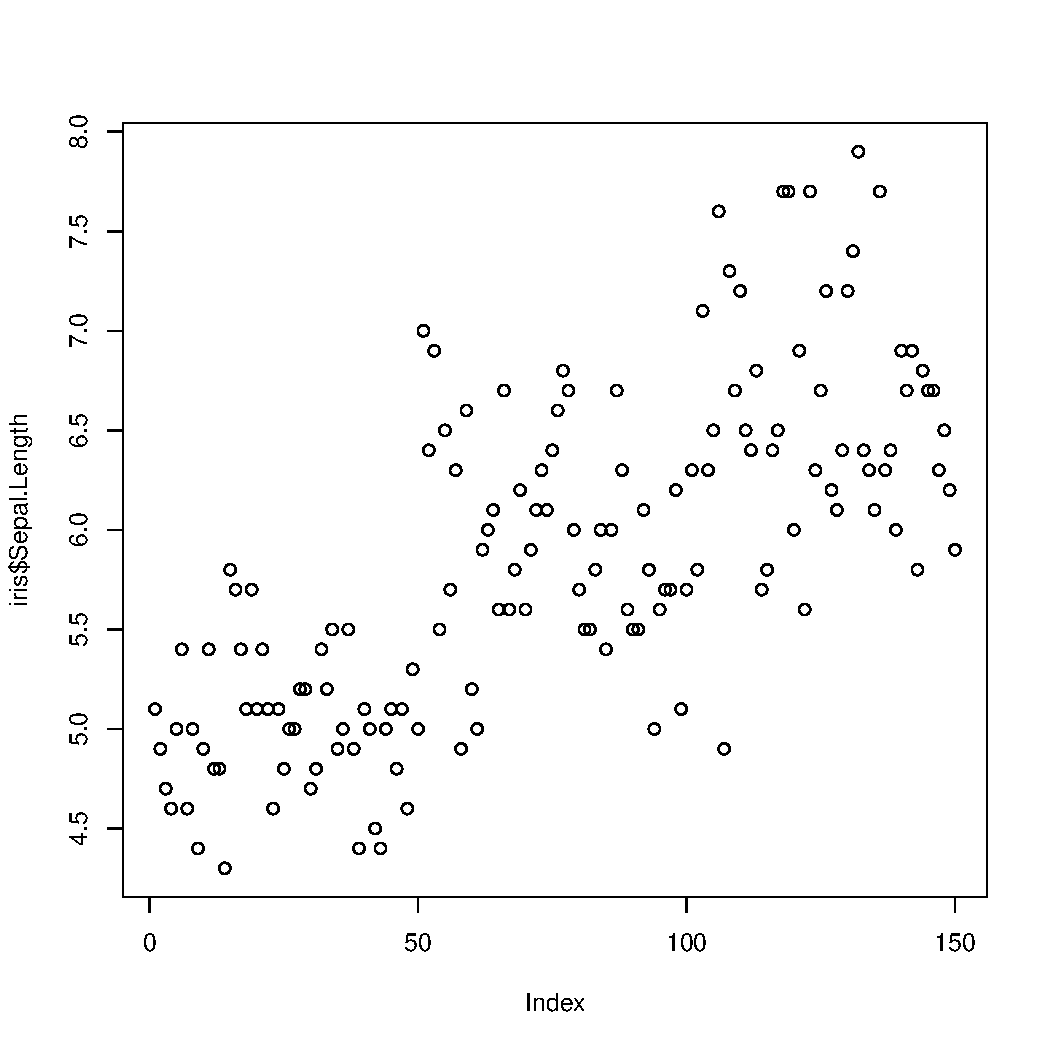
\includegraphics[width=\textwidth]{graphiques/beamer-Plot-1} } 

}



\end{knitrout}

\end{frame}


\begin{frame}[containsverbatim]
	\frametitle{Histogramme}

        Pour obtenir un histogramme, il suffit de taper~:
\begin{verbatim}
hist(iris$Sepal.Length)
\end{verbatim}

\end{frame}

\begin{frame}[containsverbatim]
	\frametitle{Histogramme}

\begin{knitrout}\footnotesize
\definecolor{shadecolor}{rgb}{0.969, 0.969, 0.969}\color{fgcolor}

{\centering \resizebox{!}{0.8\textheight}{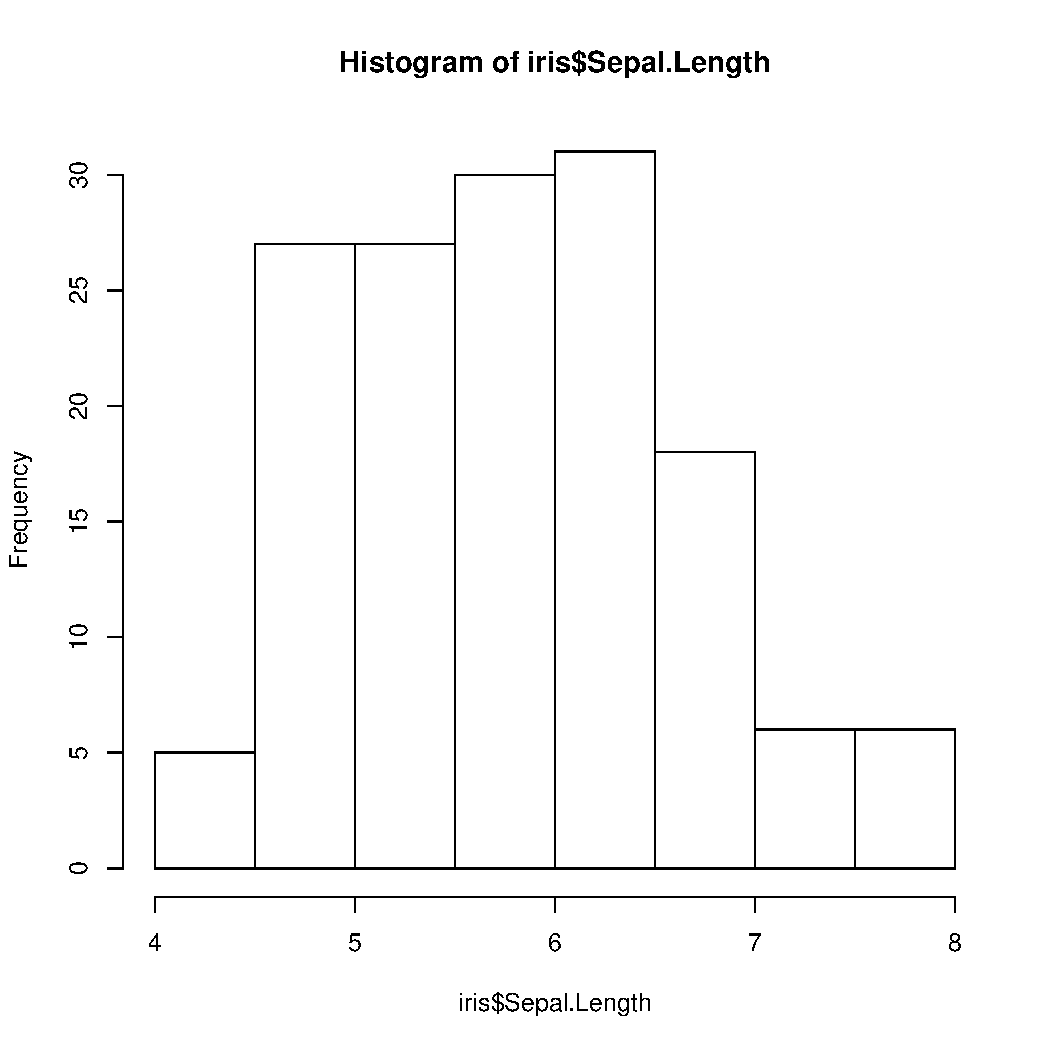
\includegraphics[width=\textwidth]{graphiques/beamer-Hist-1} } 

}



\end{knitrout}

\end{frame}

\begin{frame}[containsverbatim]
	\frametitle{Boxplots}

        Pour obtenir un boxplot, il suffit de taper~:
\begin{verbatim}
boxplot(iris$Sepal.Length)
\end{verbatim}

\end{frame}

\begin{frame}[containsverbatim]
	\frametitle{Boxplots}

\begin{knitrout}\footnotesize
\definecolor{shadecolor}{rgb}{0.969, 0.969, 0.969}\color{fgcolor}

{\centering \resizebox{!}{0.8\textheight}{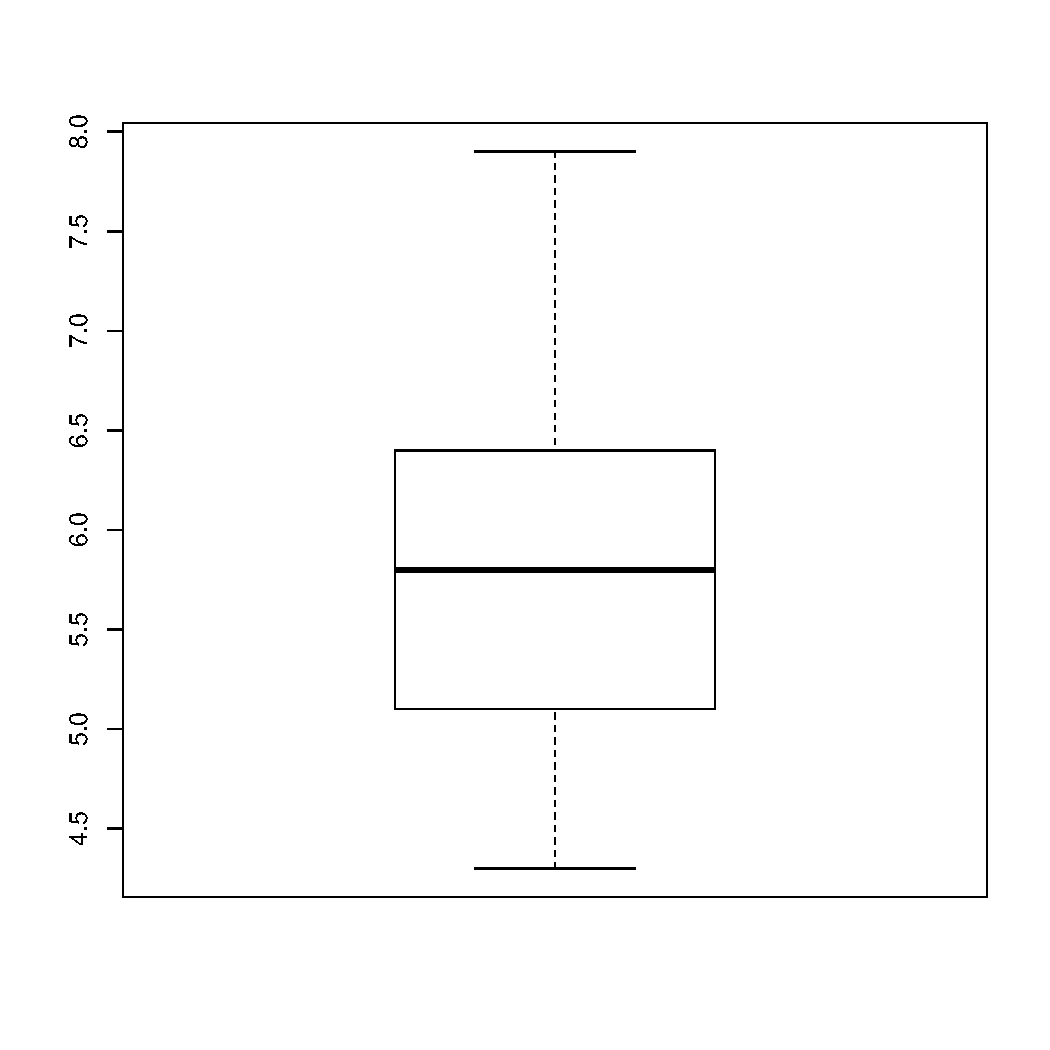
\includegraphics[width=\textwidth]{graphiques/beamer-Box1-1} } 

}



\end{knitrout}

\end{frame}

\begin{frame}[containsverbatim]
	\frametitle{Boxplots}

        Pour obtenir des boxplots de plusieurs variables d'une m�me \df, il suffit de taper :

\begin{verbatim}
boxplot(iris[,1:4])
\end{verbatim}

\end{frame}

\begin{frame}[containsverbatim]
	\frametitle{Boxplots}

\begin{knitrout}\footnotesize
\definecolor{shadecolor}{rgb}{0.969, 0.969, 0.969}\color{fgcolor}

{\centering \resizebox{!}{0.8\textheight}{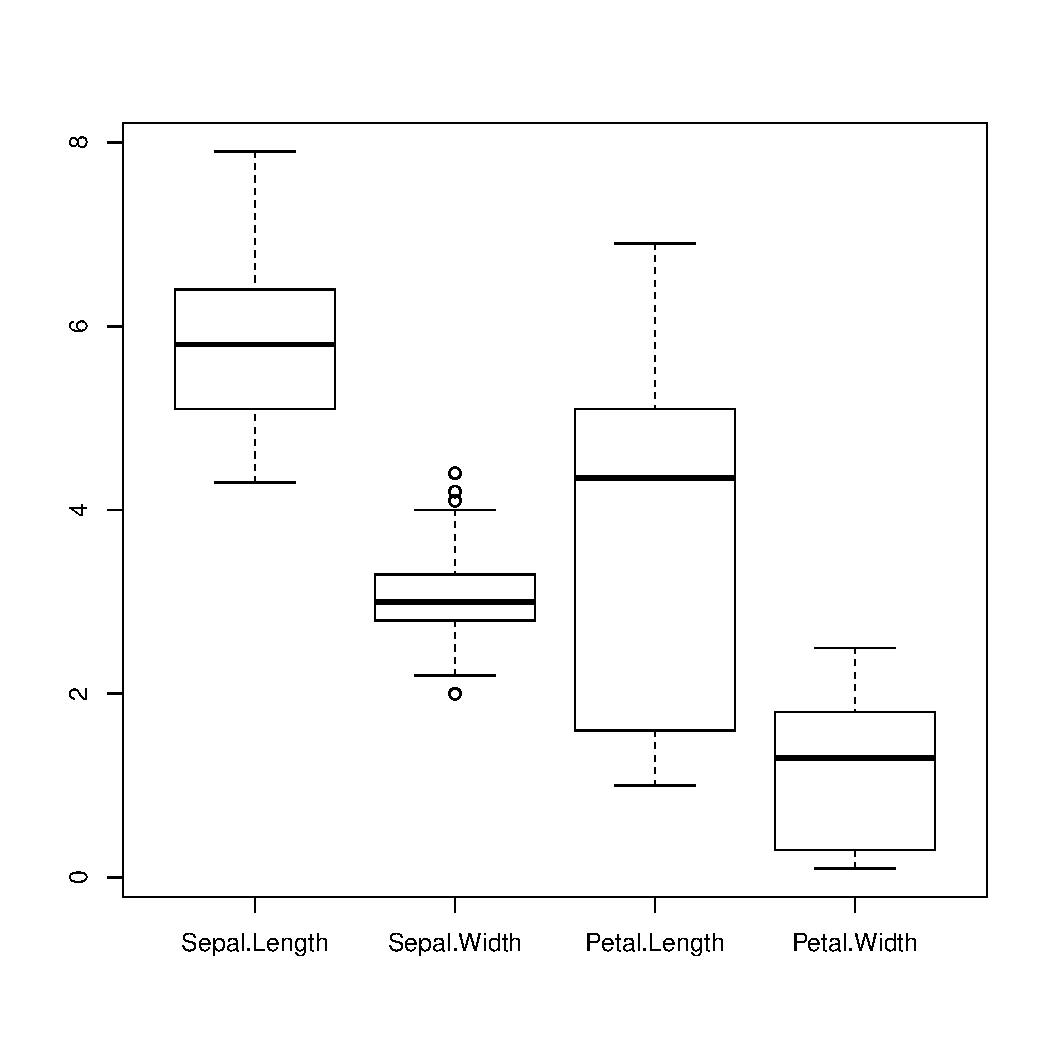
\includegraphics[width=\textwidth]{graphiques/beamer-Box2-1} } 

}



\end{knitrout}

\end{frame}

\begin{frame}[containsverbatim]
  \frametitle{Corr�lations}

        Pour analyser la covariance ou la corr�lation de deux variables (ou plus), il suffit d'appeler la fonction \emph{cov} ou \emph{cor} avec les deux variables.

\begin{knitrout}\footnotesize
\definecolor{shadecolor}{rgb}{0.969, 0.969, 0.969}\color{fgcolor}\begin{kframe}
\begin{alltt}
\hlstd{> }\hlkwd{cor}\hlstd{(cg}\hlopt{$}\hlstd{score,cg}\hlopt{$}\hlstd{plaisir)}
\end{alltt}
\begin{verbatim}
## [1] NA
\end{verbatim}
\end{kframe}
\end{knitrout}

Les m�thodes disponibles pour le calcul de la corr�lation sont celles de Pearson, Kendall et Spearman.

\end{frame}

\begin{frame}[containsverbatim]
  \frametitle{Corr�lations}

        La gestion des valeurs manquantes est particuli�re dans le cas
        des corr�lations.

        En effet on peut avoir plusieurs cas de figures, pour
        reprendre l'aide de R.

\end{frame}

\begin{frame}[containsverbatim]
	\frametitle{Corr�lations}

        Dans la majorit� des cas on utilisera le \emph{use="pairwise.complete.obs"} qui permet d'obtenir une valeur de corr�lation en pr�sence de valeurs manquantes. Dans ce cas, la corr�lation est calcul�e pour tous les couples de valeurs ne contenant pas de \emph{NA}.

        Les alternatives sont de rendre une erreur en pr�sence de \emph{NA} ou de supprimer toutes les observations contenant une valeur manquante.

\end{frame}

\begin{frame}[containsverbatim]
	\frametitle{Corr�lations}

\begin{knitrout}\footnotesize
\definecolor{shadecolor}{rgb}{0.969, 0.969, 0.969}\color{fgcolor}\begin{kframe}
\begin{alltt}
\hlstd{> }\hlkwd{cor}\hlstd{(cg}\hlopt{$}\hlstd{score,cg}\hlopt{$}\hlstd{plaisir,}\hlkwc{use}\hlstd{=}\hlstr{"pairwise.complete.obs"}\hlstd{)}
\end{alltt}
\begin{verbatim}
## [1] 0.1492273
\end{verbatim}
\end{kframe}
\end{knitrout}

        En fait, une matrice de corr�lations peut �tre cr��e en utilisant la propri�t� de \emph{cor} de se comporter diff�remment face � un objet de type \df.

\end{frame}

\begin{frame}[containsverbatim]
	\frametitle{Corr�lations}

\begin{knitrout}\footnotesize
\definecolor{shadecolor}{rgb}{0.969, 0.969, 0.969}\color{fgcolor}\begin{kframe}
\begin{alltt}
\hlstd{> }\hlkwd{cor}\hlstd{(cg[,}\hlnum{8}\hlopt{:}\hlnum{12}\hlstd{],}\hlkwc{use}\hlstd{=}\hlstr{"pairwise.complete.obs"}\hlstd{)}
\end{alltt}
\begin{verbatim}
##                 score    plaisir performance
## score       1.0000000 0.14922727  0.46193763
## plaisir     0.1492273 1.00000000  0.31990943
## performance 0.4619376 0.31990943  1.00000000
## estime_soi  0.1203776 0.12368912  0.42288147
## anx_sociale 0.1236460 0.08192793  0.04367632
##             estime_soi anx_sociale
## score        0.1203776  0.12364597
## plaisir      0.1236891  0.08192793
## performance  0.4228815  0.04367632
## estime_soi   1.0000000 -0.17216954
## anx_sociale -0.1721695  1.00000000
\end{verbatim}
\end{kframe}
\end{knitrout}

\end{frame}

\begin{frame}[containsverbatim]
	\frametitle{Corr�lations - Graphiques}

On peut �galement passer une \df � \emph{plot} pour avoir une table des corr�lations graphiques.

\begin{verbatim}
plot(iris[,1:4])
\end{verbatim}

\end{frame}

\begin{frame}[containsverbatim]
	\frametitle{Corr�lations - Graphiques}

\begin{knitrout}\footnotesize
\definecolor{shadecolor}{rgb}{0.969, 0.969, 0.969}\color{fgcolor}

{\centering \resizebox{!}{0.8\textheight}{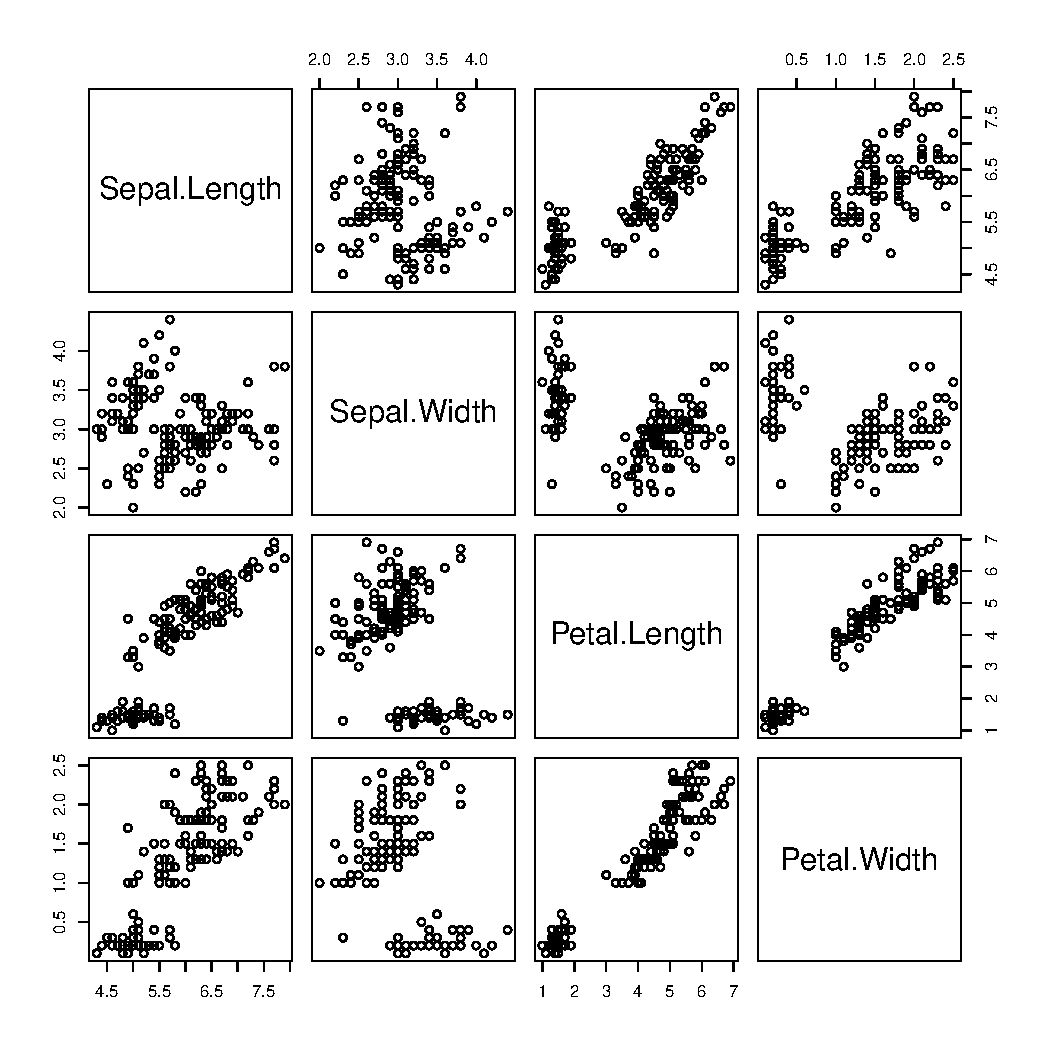
\includegraphics[width=\textwidth]{graphiques/beamer-Cor3b-1} } 

}



\end{knitrout}

\end{frame}

\section{Exemple de test statistique}

\begin{frame}[containsverbatim]
	\frametitle{Test de corr�lation}

        Le but est ici de vous illustrer un test pour
        vous montrer l'utilisation des objets.

\end{frame}

\begin{frame}[containsverbatim]
	\frametitle{Test de corr�lation}

\begin{knitrout}\footnotesize
\definecolor{shadecolor}{rgb}{0.969, 0.969, 0.969}\color{fgcolor}\begin{kframe}
\begin{alltt}
\hlstd{> }\hlkwd{cor.test}\hlstd{(cg}\hlopt{$}\hlstd{score,cg}\hlopt{$}\hlstd{plaisir,}\hlkwc{use}\hlstd{=}\hlstr{"pairwise.complete.obs"}\hlstd{)}
\end{alltt}
\begin{verbatim}
## 
## 	Pearson's product-moment correlation
## 
## data:  cg$score and cg$plaisir
## t = 22.511, df = 22250, p-value <
## 2.2e-16
## alternative hypothesis: true correlation is not equal to 0
## 95 percent confidence interval:
##  0.1363555 0.1620487
## sample estimates:
##       cor 
## 0.1492273
\end{verbatim}
\end{kframe}
\end{knitrout}

\end{frame}

\begin{frame}[containsverbatim]
	\frametitle{Test de corr�lation}

        Une sortie des r�sultats apparait mais comme la plupart des fonctions, la fonction
        \emph{cor.test} renvoie aussi un objet silencieusement. Comme il n'y a pas d'affectation R devine qu'on veut l'imprimer. Mais si on change la syntaxe~:

\begin{knitrout}\footnotesize
\definecolor{shadecolor}{rgb}{0.969, 0.969, 0.969}\color{fgcolor}\begin{kframe}
\begin{alltt}
\hlstd{> }\hlstd{montest} \hlkwb{<-} \hlkwd{cor.test}\hlstd{(cg}\hlopt{$}\hlstd{score,cg}\hlopt{$}\hlstd{plaisir,}\hlkwc{use}\hlstd{=}\hlstr{"pairwise.complete.obs"}\hlstd{)}
\end{alltt}
\end{kframe}
\end{knitrout}

\end{frame}

\begin{frame}[containsverbatim]
	\frametitle{Test de corr�lation}

        On peut acc�der aux valeurs en utilisant directement la
        fonction \emph{str} qui permet de conna�tre la structure des objets.

\end{frame}

\begin{frame}[containsverbatim]
	\frametitle{Test de corr�lation}

\begin{knitrout}\footnotesize
\definecolor{shadecolor}{rgb}{0.969, 0.969, 0.969}\color{fgcolor}\begin{kframe}
\begin{alltt}
\hlstd{> }\hlkwd{str}\hlstd{(montest)}
\end{alltt}
\begin{verbatim}
## List of 9
##  $ statistic  : Named num 22.5
##   ..- attr(*, "names")= chr "t"
##  $ parameter  : Named int 22250
##   ..- attr(*, "names")= chr "df"
##  $ p.value    : num 5.56e-111
##  $ estimate   : Named num 0.149
##   ..- attr(*, "names")= chr "cor"
##  $ null.value : Named num 0
##   ..- attr(*, "names")= chr "correlation"
##  $ alternative: chr "two.sided"
##  $ method     : chr "Pearson's product-moment correlation"
##  $ data.name  : chr "cg$score and cg$plaisir"
##  $ conf.int   : atomic [1:2] 0.136 0.162
##   ..- attr(*, "conf.level")= num 0.95
##  - attr(*, "class")= chr "htest"
\end{verbatim}
\end{kframe}
\end{knitrout}
\end{frame}

\begin{frame}[containsverbatim]
	\frametitle{Test de corr�lation}

        Par exemple, pour r�cup�rer la corr�lation et son intervalle de confiance~:

\begin{knitrout}\footnotesize
\definecolor{shadecolor}{rgb}{0.969, 0.969, 0.969}\color{fgcolor}\begin{kframe}
\begin{alltt}
\hlstd{> }\hlstd{montest}\hlopt{$}\hlstd{estimate}
\end{alltt}
\begin{verbatim}
##       cor 
## 0.1492273
\end{verbatim}
\begin{alltt}
\hlstd{> }\hlstd{montest}\hlopt{$}\hlstd{conf.int}
\end{alltt}
\begin{verbatim}
## [1] 0.1363555 0.1620487
## attr(,"conf.level")
## [1] 0.95
\end{verbatim}
\end{kframe}
\end{knitrout}

\end{frame}

\begin{frame}[containsverbatim]
	\frametitle{Autres tests}

        Les tests disponibles sous R sont nombreux dans les packages de
        base et incalculables si on tient compte des paquets~: Student,
        Wilcoxon, $\chi^2$, Bartlett, Fisher, ...

        Tous, ou presque, fonctionnent sur le m�me principe.

\end{frame}


\section{Statistiques descriptives : variables qualitatives}

\begin{frame}[containsverbatim]
	\frametitle{Les donn�es patient}

        Ce sont des donn�es recolt�es par une pharmacienne sur
        dossiers dans deux hopitaux.

        Les donn�es portent sur le traitement de la douleur chez
        l'enfant. Le but est de d�terminer la qualit� de la prise en
        charge de la douleur dans ces hopitaux.

        Pour cela les �valuations de la douleur se font sur une
        �chelle de 0 � 100.

        Les pathologies (CIM2) concern�es sont cod�es de 1 � 4, de plus en plus
        grave (appendicite � arthrod�se).

\end{frame}

\begin{frame}[containsverbatim]
	\frametitle{Les donn�es patient}

% Table generated by Excel2LaTeX from sheet 'Feuil1'

\begin{table}[htbp]
  \centering
  \scalebox{0.7}{
    \begin{tabular}{rr}
    \addlinespace
    \toprule
    {\bf Variable} & {\bf Description} \\
    \midrule
    UID   & Identifiant \\
    Hopital & Hopital ( A ou B) \\
    Sexe  & Sexe du patient \\
    Poids & Poids du patient \\
    Vitaux & Nombres de prises des signes vitaux \\
    CIM2  & Pathologie (de 1 � 4, de plus en plus grave) \\
    age   & �ge du patient \\
    dureeopmin & Dur�e de l'op�ration en minutes \\
    postopj & Nombres de jours post-op�ratoires \\
    scoliose & Pr�sence d'une scoliose \\
    drepano & Enfant souffrant d'une dr�panocytose/sph�rocytose \\
    ACP   & Pompe � morphine administr�e \\
    peridurale & Injection p�ridurale \\
    periACP & Pompe � morphine administr�e en p�ridurale \\
    nbttt & Nombre de traitements contre la douleur \\
    totalechelle & Total des �chelles de la la douleur \\
    nbechelle & Nombre de prises d'�chelles de douleur \\
    \bottomrule
    \end{tabular}
   }
\end{table}


\end{frame}

\begin{frame}[containsverbatim]
	\frametitle{Tableaux de contingence}

        Il suffit d'utiliser la fonction \emph{table}.

\begin{knitrout}\footnotesize
\definecolor{shadecolor}{rgb}{0.969, 0.969, 0.969}\color{fgcolor}\begin{kframe}
\begin{alltt}
\hlstd{> }\hlstd{patient} \hlkwb{<-} \hlkwd{read.csv2}\hlstd{(}\hlstr{"data/patient.csv"}\hlstd{)}
\hlstd{> }\hlkwd{table}\hlstd{(patient}\hlopt{$}\hlstd{sexe)}
\end{alltt}
\begin{verbatim}
## 
##  Feminin Masculin 
##      101       75
\end{verbatim}
\end{kframe}
\end{knitrout}

\end{frame}

\begin{frame}[containsverbatim]
	\frametitle{Tableaux de contingence}

        Ces tableaux peuvent �tre � 2 niveaux~:

\begin{knitrout}\footnotesize
\definecolor{shadecolor}{rgb}{0.969, 0.969, 0.969}\color{fgcolor}\begin{kframe}
\begin{alltt}
\hlstd{> }\hlkwd{table}\hlstd{(patient}\hlopt{$}\hlstd{sexe,patient}\hlopt{$}\hlstd{CIM2)}
\end{alltt}
\begin{verbatim}
##           
##             1  2  3  4
##   Feminin  18 24 18 41
##   Masculin 26 22 18  9
\end{verbatim}
\end{kframe}
\end{knitrout}

\end{frame}

\begin{frame}[containsverbatim]
	\frametitle{Tableaux de contingence}

        Comme les colonnes ne sont pas nomm�es cela peut �tre
        difficile de s'y retrouver si les variables ont les m�mes modalit�s.

        Il suffit dans ce cas l� de modifier la syntaxe~:

\begin{knitrout}\footnotesize
\definecolor{shadecolor}{rgb}{0.969, 0.969, 0.969}\color{fgcolor}\begin{kframe}
\begin{alltt}
\hlstd{> }\hlkwd{table}\hlstd{(}\hlkwc{Sexe}\hlstd{=patient}\hlopt{$}\hlstd{sexe,}\hlkwc{CIM2}\hlstd{=patient}\hlopt{$}\hlstd{CIM2)}
\end{alltt}
\begin{verbatim}
##           CIM2
## Sexe        1  2  3  4
##   Feminin  18 24 18 41
##   Masculin 26 22 18  9
\end{verbatim}
\end{kframe}
\end{knitrout}

\end{frame}

\begin{frame}[containsverbatim]
	\frametitle{Exportation de tableaux de contingence}

        Pour l'exportation des tableaux, elle peut se faire avec~:
        \begin{itemize}
          \item \emph{xtable}
          \item la fonction clipcopy de \emph{questionr}
          \item sous forme de CSV
        \end{itemize}
        
        Dans ce dernier cas, l'aspect de la table export�e sera donc diff�rent car il y a une conversion vers une \df.

\end{frame}

\begin{frame}[containsverbatim]
	\frametitle{Exportation de tableaux de contingence}

\begin{knitrout}\footnotesize
\definecolor{shadecolor}{rgb}{0.969, 0.969, 0.969}\color{fgcolor}\begin{kframe}
\begin{alltt}
\hlstd{> }\hlkwd{as.data.frame}\hlstd{(}\hlkwd{table}\hlstd{(}\hlkwc{Sexe}\hlstd{=patient}\hlopt{$}\hlstd{sexe,}\hlkwc{CIM2}\hlstd{=patient}\hlopt{$}\hlstd{CIM2))}
\end{alltt}
\begin{verbatim}
##       Sexe CIM2 Freq
## 1  Feminin    1   18
## 2 Masculin    1   26
## 3  Feminin    2   24
## 4 Masculin    2   22
## 5  Feminin    3   18
## 6 Masculin    3   18
## 7  Feminin    4   41
## 8 Masculin    4    9
\end{verbatim}
\end{kframe}
\end{knitrout}

\end{frame}

\begin{frame}[containsverbatim]
	\frametitle{Exportation de tableaux de contingence (ancienne version)}

        Il y a une astuce pour contourner le probl�me. La
        classe \emph{table} a la m�me structure interne qu'une
        \emph{matrix}. Alors on berne R.

\begin{knitrout}\footnotesize
\definecolor{shadecolor}{rgb}{0.969, 0.969, 0.969}\color{fgcolor}\begin{kframe}
\begin{alltt}
\hlstd{> }\hlstd{tableau} \hlkwb{<-} \hlstd{(}\hlkwd{table}\hlstd{(}\hlkwc{Sexe}\hlstd{=patient}\hlopt{$}\hlstd{sexe,}\hlkwc{CIM2}\hlstd{=patient}\hlopt{$}\hlstd{CIM2))}
\hlstd{> }\hlkwd{class}\hlstd{(tableau)}
\end{alltt}
\begin{verbatim}
## [1] "table"
\end{verbatim}
\begin{alltt}
\hlstd{> }\hlkwd{class}\hlstd{(tableau)} \hlkwb{<-} \hlstr{"matrix"}
\hlstd{> }\hlkwd{class}\hlstd{(tableau)}
\end{alltt}
\begin{verbatim}
## [1] "matrix"
\end{verbatim}
\end{kframe}
\end{knitrout}

\end{frame}

\begin{frame}[containsverbatim]
	\frametitle{Exportation de tableaux de contingence (version correcte)}

        Depuis la premi�re version du cours, il y a maintenant un contournement dans R~:

\begin{knitrout}\footnotesize
\definecolor{shadecolor}{rgb}{0.969, 0.969, 0.969}\color{fgcolor}\begin{kframe}
\begin{alltt}
\hlstd{> }\hlstd{tableau} \hlkwb{<-} \hlstd{(}\hlkwd{table}\hlstd{(}\hlkwc{Sexe}\hlstd{=patient}\hlopt{$}\hlstd{sexe,}\hlkwc{CIM2}\hlstd{=patient}\hlopt{$}\hlstd{CIM2))}
\hlstd{> }\hlkwd{as.data.frame.matrix}\hlstd{(tableau)}
\end{alltt}
\begin{verbatim}
##           1  2  3  4
## Feminin  18 24 18 41
## Masculin 26 22 18  9
\end{verbatim}
\end{kframe}
\end{knitrout}

\end{frame}

\begin{frame}[containsverbatim]
	\frametitle{Marges sur les tableaux}

        On peut ajouter les marges avec la fonction addmargins~:

\end{frame}

\begin{frame}[containsverbatim]
	\frametitle{Marges sur les tableaux}

\begin{knitrout}\footnotesize
\definecolor{shadecolor}{rgb}{0.969, 0.969, 0.969}\color{fgcolor}\begin{kframe}
\begin{alltt}
\hlstd{> }\hlkwd{addmargins}\hlstd{(tableau,}\hlnum{1}\hlstd{)}
\end{alltt}
\begin{verbatim}
##           CIM2
## Sexe        1  2  3  4
##   Feminin  18 24 18 41
##   Masculin 26 22 18  9
##   Sum      44 46 36 50
\end{verbatim}
\end{kframe}
\end{knitrout}

\end{frame}

\begin{frame}[containsverbatim]
	\frametitle{Marges sur les tableaux}

\begin{knitrout}\footnotesize
\definecolor{shadecolor}{rgb}{0.969, 0.969, 0.969}\color{fgcolor}\begin{kframe}
\begin{alltt}
\hlstd{> }\hlkwd{addmargins}\hlstd{(tableau,}\hlnum{2}\hlstd{)}
\end{alltt}
\begin{verbatim}
##           CIM2
## Sexe         1   2   3   4 Sum
##   Feminin   18  24  18  41 101
##   Masculin  26  22  18   9  75
\end{verbatim}
\end{kframe}
\end{knitrout}

\end{frame}

\begin{frame}[containsverbatim]
	\frametitle{Marges sur les tableaux}

\begin{knitrout}\footnotesize
\definecolor{shadecolor}{rgb}{0.969, 0.969, 0.969}\color{fgcolor}\begin{kframe}
\begin{alltt}
\hlstd{> }\hlkwd{addmargins}\hlstd{(tableau,}\hlnum{1}\hlopt{:}\hlnum{2}\hlstd{)}
\end{alltt}
\begin{verbatim}
##           CIM2
## Sexe         1   2   3   4 Sum
##   Feminin   18  24  18  41 101
##   Masculin  26  22  18   9  75
##   Sum       44  46  36  50 176
\end{verbatim}
\end{kframe}
\end{knitrout}

\end{frame}

\begin{frame}[containsverbatim]
	\frametitle{Tableau de proportion}

        Cette fois c'est la fonction \emph{prop.table} qu'on appelle
        en utilisant une table d�j� cr��e~:

\begin{knitrout}\footnotesize
\definecolor{shadecolor}{rgb}{0.969, 0.969, 0.969}\color{fgcolor}\begin{kframe}
\begin{alltt}
\hlstd{> }\hlkwd{prop.table}\hlstd{(tableau,}\hlnum{1}\hlstd{)}
\end{alltt}
\begin{verbatim}
##           CIM2
## Sexe               1         2         3
##   Feminin  0.1782178 0.2376238 0.1782178
##   Masculin 0.3466667 0.2933333 0.2400000
##           CIM2
## Sexe               4
##   Feminin  0.4059406
##   Masculin 0.1200000
\end{verbatim}
\end{kframe}
\end{knitrout}

\end{frame}


\begin{frame}[containsverbatim]
	\frametitle{Proportions dans les tableaux}

\begin{knitrout}\footnotesize
\definecolor{shadecolor}{rgb}{0.969, 0.969, 0.969}\color{fgcolor}\begin{kframe}
\begin{alltt}
\hlstd{> }\hlkwd{prop.table}\hlstd{(tableau,}\hlnum{2}\hlstd{)}
\end{alltt}
\begin{verbatim}
##           CIM2
## Sexe               1         2         3
##   Feminin  0.4090909 0.5217391 0.5000000
##   Masculin 0.5909091 0.4782609 0.5000000
##           CIM2
## Sexe               4
##   Feminin  0.8200000
##   Masculin 0.1800000
\end{verbatim}
\end{kframe}
\end{knitrout}

\end{frame}

\begin{frame}[containsverbatim]
	\frametitle{Proportions dans les tableaux}

        On peut combiner les deux...

\begin{knitrout}\footnotesize
\definecolor{shadecolor}{rgb}{0.969, 0.969, 0.969}\color{fgcolor}\begin{kframe}
\begin{alltt}
\hlstd{> }\hlkwd{addmargins}\hlstd{(}\hlkwd{prop.table}\hlstd{(tableau),}\hlnum{1}\hlopt{:}\hlnum{2}\hlstd{)}
\end{alltt}
\begin{verbatim}
##           CIM2
## Sexe                1          2          3
##   Feminin  0.10227273 0.13636364 0.10227273
##   Masculin 0.14772727 0.12500000 0.10227273
##   Sum      0.25000000 0.26136364 0.20454545
##           CIM2
## Sexe                4        Sum
##   Feminin  0.23295455 0.57386364
##   Masculin 0.05113636 0.42613636
##   Sum      0.28409091 1.00000000
\end{verbatim}
\end{kframe}
\end{knitrout}

\end{frame}

\begin{frame}[containsverbatim]
  \frametitle{Autres fonctions}
  
  Les autres fonctions dans les tableaux de base sont \emph{ftable}, \emph{tabulate}, \emph{xtabs}, \dots Chacun a sa petite sp�cificit�.
  
  Dans les packages, il existe pl�thore de fonctions pour calculer des tableaux crois�s. Notamment des versions qui permettent d'ajuster la pr�sentation comme dans \emph{questionr}.

\end{frame}


\end{document}


\documentclass{beamer}\usepackage[]{graphicx}\usepackage[]{color}
%% maxwidth is the original width if it is less than linewidth
%% otherwise use linewidth (to make sure the graphics do not exceed the margin)
\makeatletter
\def\maxwidth{ %
  \ifdim\Gin@nat@width>\linewidth
    \linewidth
  \else
    \Gin@nat@width
  \fi
}
\makeatother

\definecolor{fgcolor}{rgb}{0.345, 0.345, 0.345}
\newcommand{\hlnum}[1]{\textcolor[rgb]{0.686,0.059,0.569}{#1}}%
\newcommand{\hlstr}[1]{\textcolor[rgb]{0.192,0.494,0.8}{#1}}%
\newcommand{\hlcom}[1]{\textcolor[rgb]{0.678,0.584,0.686}{\textit{#1}}}%
\newcommand{\hlopt}[1]{\textcolor[rgb]{0,0,0}{#1}}%
\newcommand{\hlstd}[1]{\textcolor[rgb]{0.345,0.345,0.345}{#1}}%
\newcommand{\hlkwa}[1]{\textcolor[rgb]{0.161,0.373,0.58}{\textbf{#1}}}%
\newcommand{\hlkwb}[1]{\textcolor[rgb]{0.69,0.353,0.396}{#1}}%
\newcommand{\hlkwc}[1]{\textcolor[rgb]{0.333,0.667,0.333}{#1}}%
\newcommand{\hlkwd}[1]{\textcolor[rgb]{0.737,0.353,0.396}{\textbf{#1}}}%

\usepackage{framed}
\makeatletter
\newenvironment{kframe}{%
 \def\at@end@of@kframe{}%
 \ifinner\ifhmode%
  \def\at@end@of@kframe{\end{minipage}}%
  \begin{minipage}{\columnwidth}%
 \fi\fi%
 \def\FrameCommand##1{\hskip\@totalleftmargin \hskip-\fboxsep
 \colorbox{shadecolor}{##1}\hskip-\fboxsep
     % There is no \\@totalrightmargin, so:
     \hskip-\linewidth \hskip-\@totalleftmargin \hskip\columnwidth}%
 \MakeFramed {\advance\hsize-\width
   \@totalleftmargin\z@ \linewidth\hsize
   \@setminipage}}%
 {\par\unskip\endMakeFramed%
 \at@end@of@kframe}
\makeatother

\definecolor{shadecolor}{rgb}{.97, .97, .97}
\definecolor{messagecolor}{rgb}{0, 0, 0}
\definecolor{warningcolor}{rgb}{1, 0, 1}
\definecolor{errorcolor}{rgb}{1, 0, 0}
\newenvironment{knitrout}{}{} % an empty environment to be redefined in TeX

\usepackage{alltt}
\usetheme[compress]{Singapore}
\useoutertheme{miniframes}

% \documentclass{beamer}
%\usetheme{Warsaw}

% Pour les documents en francais...
	\usepackage[latin1]{inputenc}
	\usepackage[french]{babel}
	\usepackage[french]{varioref}

% Math�matiques
	\usepackage{amsmath}

% Caracteres speciaux suppl�mentaires
	\usepackage{latexsym,amsfonts}

% A documenter
	\usepackage{moreverb}

% Macros pour les paquets
	\usepackage{array}  			% N�cessaires pour les tableaux de la macro Excel.

% Outil suppl�mentaire pour les tableaux
	\usepackage{multirow}
	\usepackage{booktabs}
	\usepackage{xcolor} % alternating row colors in table, incompatible avec certains modules
	\usepackage{longtable}
	\usepackage{colortbl}

% Pour ins�rer des graphiques
	\usepackage{graphicx} 			% Graphique simples
	\usepackage{subfigure}			% Graphiques multiples

% Pour ins�rer des couleurs
	\usepackage{color}

% Rotation des objets et des pages
%	\usepackage{rotating}
%	\usepackage{lscape}

% Pour insrer du code source, LaTeX ou SAS par exemple.
	\usepackage{verbatim}
        \usepackage{moreverb}
	\usepackage{listings}
	\usepackage{fancyvrb}

%	\lstset{language=SAS,numbers=left}		% Par dfaut le listing est en SAS

% Pour ins�rer des hyperliens
  \usepackage{hyperref}

% American Psychological Association (for bibliographic references).
	\usepackage{apacite}

% Pour l'utilisation des macros
	\usepackage{xspace}

% Pour l'utilisation de notes en fin de document.
%	\usepackage{endnotes}

% Array
%	\usepackage{multirow}
%	\usepackage{booktabs}

% Rotation
%	\usepackage{rotating}

% En t�tes et pieds de pages
%	\usepackage{fancyhdr}
%	\usepackage{lastpage}


% Page layout

% By LaTeX commands
%\setlength{\oddsidemargin}{0cm}
%\setlength{\textwidth}{16cm}
%\setlength{\textheight}{24cm}
%\setlength{\topmargin}{-1cm}
%\setlength{\marginparsep}{0.2cm}

% fancyheader parameters
%\pagestyle{fancy}

%\fancyfoot[L]{{\small Formation \LaTeX, DEPP}}
%\fancyfoot[c]{}
%\fancyfoot[R]{{\small \thepage/\pageref{LastPage}}}

%\fancyhead[L]{}
%\fancyhead[c]{}
%\fancyhead[R]{}

% Pour ins�rer des dessins de Linux
\newcommand{\LinuxA}{\includegraphics[height=0.5cm]{Graphiques/linux.png}}
\newcommand{\LinuxB}{\includegraphics[height=0.5cm]{Graphiques/linux.png}\xspace}

% Macro pour les petits dessins pour les diff�rents OS.
\newcommand{\Windows}{\emph{Windows}\xspace}
\newcommand{\Mac}{\emph{Mac OS X}\xspace}
\newcommand{\Linux}{\emph{Linux}\xspace}
\newcommand{\MikTeX}{MiK\tex\xspace}
\newcommand{\latex}{\LaTeX\xspace}


\newcommand{\df}{\emph{data.frame}\xspace}
\newcommand{\liste}{\emph{list}\xspace}
\newcommand{\cad}{c'est-�-dire\xspace}

% Titre
\title{Introduction � R}
\author{Pascal Bessonneau}
%\institute{DEPP}
\date{06/2015}


\subtitle{Comprendre et trouver de l'aide}


\newcommand{\hreff}[2]{\underline{\href{#1}{#2}\xspace}}




\IfFileExists{upquote.sty}{\usepackage{upquote}}{}
\begin{document}

\begin{frame}
	\maketitle
\end{frame}

\begin{frame}
	\tableofcontents
\end{frame}

% Begin document %%%%%%%%%%%%%%%%%%%%%%%%%%%%%%%%%%%%%%%%%%%%%%%%%%%%%%%%%%%%%%%%%%%%%%%%%%%%%%%%%%



\section{Recherche directe sur une fonction}

\begin{frame}[containsverbatim]
	\frametitle{Recherche directe sur une fonction}

        La recherche se fait � l'aide de la syntaxe \emph{?fonction} ou bien \emph{help(fonction)}.

        La syntaxe de l'aide obtenue est th�oriquement assez constante d'un paquet � un
        autre car elle est bas�e sur un format
        standard~:\emph{.Rd}. Ce format ressemble � un fichier \latex.

\end{frame}

\begin{frame}[containsverbatim]
	\frametitle{Recherche directe sur une fonction}

        Dans l'aide, on trouvera les parties suivantes~:
        \begin{description}
          \item[D�but] le nom de la fonction et le nom du paquet auquelle elle appartient
          \item[Description] une description sommaire de la fonction
          \item[Usage] la fa�on d'appeler la fonction
          \item[Arguments] les arguments possibles pour la fonction
          \item[Details] les d�tails sur le fonctionnement de la fonction
        \end{description}

\end{frame}

\begin{frame}[containsverbatim]
	\frametitle{Recherche directe sur une fonction}

        \begin{description}
          \item[Value] le type d'objet et/ou les valeurs retourn�es
          \item[Note] des remarques g�n�rales
          \item[References] les r�f�rences bibliographiques
          \item[See also] des liens vers des fonctions connexes
          \item[Examples] des exemples fonctionnels de la fonction
        \end{description}

\end{frame}

\begin{frame}[containsverbatim]
	\frametitle{Recherche directe sur une fonction}

        La partie la plus difficile est la partie \emph{Usage}. En
        effet c'est dans cette partie qu'on va lire la fa�on d'appeler
        la fonction selon le type de l'objet pass�.

\end{frame}

\begin{frame}[containsverbatim]
	\frametitle{La partie Usage de t.test}

\begin{verbatimtab}
Usage

t.test(x, ...)

## Default S3 method:
t.test(x, y = NULL,
       alternative = c("two.sided", "less", "greater"),
       mu = 0, paired = FALSE, var.equal = FALSE,
       conf.level = 0.95, ...)

## S3 method for class 'formula'
t.test(formula, data, subset, na.action, ...)
\end{verbatimtab}

\end{frame}

\begin{frame}[containsverbatim]
	\frametitle{Recherche directe sur une fonction}

        La premi�re description indique l'appel minimal.

        Dans le second cas, la syntaxe indiqu�e correspond � l'appel de la
        fonction lorsque l'objet est tel que pr�cis� dans l'aide.

        Le troisi�me cas indique le comportement de la fonction si
        l'objet est type \emph{formula}.

\end{frame}

\begin{frame}[containsverbatim]
	\frametitle{La partie \emph{Usage} de \emph{t.test}}

        C'est dans cette partie qu'on retrouve les arguments possibles
        de la fonction. Parfois, ils ne sont pas tous list�s.

        Les arguments sans valeurs par d�faut sont des arguments obligatoires.

        Les arguments avec une valeur par exemple \emph{paired =
          FALSE} sont des arguments facultatifs car ils prennent
        comme valeurs par d�faut la valeur indiqu�e.

\end{frame}

\begin{frame}[containsverbatim]
	\frametitle{La partie \emph{Usage} de \emph{t.test}}

        Les arguments sont positionnels, \cad
        qu'on peut les passer � la fonction dans l'ordre o� ils sont
        cit�s dans la rubrique \emph{Usage}.

        Toutefois on peut aussi utiliser un m�canisme d'appel par nom~: dans ce
        cas on passe le nom de l'argument suivi de sa valeur.

\end{frame}

\begin{frame}[containsverbatim]
	\frametitle{La partie \emph{Usage} de \emph{t.test}}

        Dans les sp�cifications d'un paquet R, il est indiqu� que les
        exemples doivent �tre fonctionnels (sauf si \emph{Not run} est pr�cis� en commentaire).

        D'ailleurs on peut les ex�cuter en tapant \emph{example(fonction)}

\end{frame}

\begin{frame}[containsverbatim]
	\frametitle{La partie \emph{Usage} de \emph{t.test}}

        Toutes ces syntaxes suivantes sont �quivalentes~:

\begin{knitrout}\footnotesize
\definecolor{shadecolor}{rgb}{0.969, 0.969, 0.969}\color{fgcolor}\begin{kframe}
\begin{alltt}
\hlstd{x} \hlkwb{<-} \hlkwd{rnorm}\hlstd{(}\hlnum{1000}\hlstd{)}
\hlkwd{t.test}\hlstd{(x,}\hlkwc{conf.level}\hlstd{=}\hlnum{0.8}\hlstd{)}
\hlkwd{t.test}\hlstd{(}\hlkwc{conf}\hlstd{=}\hlnum{0.8}\hlstd{,}\hlkwc{x}\hlstd{=x)}
\end{alltt}
\end{kframe}
\end{knitrout}

\end{frame}

\begin{frame}[containsverbatim]
	\frametitle{La partie \emph{Usage} de \emph{t.test}}

        Il est � noter que l'aide de R est parfois cryptique dans les
        paquets de base. C'est notamment le cas de la fonction
        \emph{plot}. La fonction a tellement de possibilit�s que l'aide ne fournit
        que les �l�ments de base.

\end{frame}

\begin{frame}[containsverbatim]
	\frametitle{\emph{S3} et fonctions}

        R est un langage pseudo-objet pour le \emph{S3}. C'est-�-dire que certaines fonctions vont se comporter
        diff�remment selon le type d'objet qu'on lui passe.

        Cela repose sur l'�valuation de la classe de l'objet au niveau
        de l'appel ou de l'affichage...

\end{frame}

\begin{frame}[containsverbatim]
	\frametitle{\emph{S3} et fonctions}

        Pour conna�tre la classe d'un objet il faut taper~:
\begin{knitrout}\footnotesize
\definecolor{shadecolor}{rgb}{0.969, 0.969, 0.969}\color{fgcolor}\begin{kframe}
\begin{alltt}
\hlkwd{class}\hlstd{(iris)}
\end{alltt}
\begin{verbatim}
## [1] "data.frame"
\end{verbatim}
\end{kframe}
\end{knitrout}

\end{frame}

\begin{frame}[containsverbatim]
	\frametitle{\emph{S3} et fonctions}

        Pour conna�tre les fonctions g�n�riques utilisables avec un type d'objet
        donn�, il suffit de taper la commande~:
\begin{knitrout}\footnotesize
\definecolor{shadecolor}{rgb}{0.969, 0.969, 0.969}\color{fgcolor}\begin{kframe}
\begin{alltt}
\hlkwd{methods}\hlstd{(}\hlkwc{class}\hlstd{=}\hlstr{"data.frame"}\hlstd{)}
\end{alltt}
\begin{verbatim}
##  [1] aggregate     anyDuplicated as.data.frame
##  [4] as.list       as.matrix     by           
##  [7] cbind         coerce        [<-          
## [10] [             [[<-          [[           
## [13] $<-           $             dim          
## [16] dimnames<-    dimnames      droplevels   
## [19] duplicated    edit          format       
## [22] formula       head          initialize   
## [25] is.na         Math          merge        
## [28] na.exclude    na.omit       Ops          
## [31] plot          print         prompt       
## [34] rbind         row.names<-   row.names    
## [37] rowsum        show          slotsFromS3  
## [40] split<-       split         stack        
## [43] str           subset        summary      
## [46] Summary       tail          t            
## [49] transform     unique        unstack      
## [52] within       
## see '?methods' for accessing help and source code
\end{verbatim}
\end{kframe}
\end{knitrout}

\end{frame}

\section{La recherche sur une fonctionnalit�}

\begin{frame}[containsverbatim]
	\frametitle{La recherche par mots clefs via la console}

        R permet dans la console de chercher les fonctions associ�es �
        un mot-clef � l'aide la commande \emph{help.search} ou \emph{??}.

        Cette fonction ne cherche que les occurences des mots dans les
        champs \emph{noms} et \emph{description} et seulement pour les paquets {\bf install�s}.

        Pour r�ponse, R renvoie les noms des fonctions suivis des
        paquets correspondants et enfin d'un description br�ve des fonctions.

\end{frame}

\begin{frame}[containsverbatim]
	\frametitle{La recherche par mots clefs sur internet}

        Sur la \href{http://cran.at.r-project.org/}{page} des packages
        du CRAN, on peut d�j� chercher et trouver beaucoup d'informations.

        L'autre m�thode est d'utiliser le moteur de recherche
        \href{http://www.rseek.org/}{RSeek} qui
        ne r�f�rencie que les pages sur R. Le moteur cherche dans les
        newsgroups de R, les documents, ...

\end{frame}

\begin{frame}[containsverbatim]
	\frametitle{La recherche par mots clefs sur internet}

        Outre les newsgroups, des sites de type Quora,
        d�di�s � R ou aux statistiques, existent et permettent de
        poser des questions. On citera par exemple~:
        \begin{description}
          \item
            [\href{http://stats.stackexchange.com/}{StatExchange ou
              Cross Validated}]
            orient� statistiques
          \item
            [\href{http://stackoverflow.com/questions/tagged/r}{StackOverFlow}]
            orient� programmation

       \end{description}

\end{frame}

\section{Les documents sur R}

\begin{frame}[containsverbatim]
	\frametitle{La recherche de tutoriels et de documents}

        Un gros volume de documentation est disponible sur la
        \href{http://www.r-project.org/}{page} du projet dans la
        partie \emph{Documentation}.

        On trouvera �galement un journal sur le site de R.

        Enfin beaucoup de paquets sont d�crits dans le \href{http://www.jstatsoft.org/}{Journal of statistical software}.

\end{frame}

\section{Les RUGs}

\begin{frame}[containsverbatim]
	\frametitle{Les groupes d'utilisateurs}

        Les R Users Groups ou \emph{RUGs} sont tr�s actifs... Deux
        sont pr�sents dans la r�gion parisienne~:
        \begin{description}
          \item [\href{http://rug.mnhn.fr/semin-r/}{Semin-R}] INED, MNHN, ...
          \item [\href{https://fltaur.wordpress.com/}{FLtauR}] INSEE, ...
        \end{description}

        De nombreux documents, issus des conf�rences notamment, sont
        disponibles sur leurs sites. Le groupe \emph{Semin-R} a une mailing-list pour poser des questions ainsi que les utilisateurs de R en sciences sociales \href{http://alea.fr.eu.org/pages/R-soc}{R-soc}.

\end{frame}

\begin{frame}[containsverbatim]
	\frametitle{Les groupes d'utilisateurs}

  Le groupe \emph{Semin-R} a une mailing-list pour poser des questions ainsi que les utilisateurs de R en sciences sociales \href{http://alea.fr.eu.org/pages/R-soc}{R-soc}.
  
  Les r�ponses � ces groupes seront \og~plus douces~\fg si vous posez une question qui a d�j� �t� pos� (que sur les \href{http://www.r-project.org/mail.html}{mailing-list officielles de R}).
  
  A noter que de nombreux paquets ont une mailing-lists ou un groupe Google pour obtenir de l'aide sur un paquet pr�cis~: \href{https://groups.google.com/forum/#!forum/knitr}{knitr}, \href{https://groups.google.com/forum/#!forum/factominer-users}{FactoMineR}, \href{https://groups.google.com/forum/#!forum/ggplot2}{ggplot2}, \dots

\end{frame}

\begin{frame}[containsverbatim]
	\frametitle{Les conf�rences}

        Une r�union des utilisateurs fran�ais est organis� maintenant
        chaque ann�e. Cette ann�e (2015) � \href{http://r2015-grenoble.sciencesconf.org/}{Grenoble} sur les jours de la formation.

        Les conf�rences { \bfseries UseR! } sont mondiales. En 2015,
        d�but juillet en \href{http://user2015.math.aau.dk/}{Aalborg} qui comme chacun sait est au Danemark.

\end{frame}

\end{document}

\section{Les diff�rentres m�thodes}

  \subsection{Les m�thodes}
  
  Tout d'abord R fournit des fonctions permettant de produire des graphiques 
  simples gr�ce � quelques fonctions de base.
  
  Ces graphiques dits "de base" sont assez simples � manipuler et � produire.
  
  Apr�s des m�thodes plus avanc�s mais demandant beaucoup plus de dext�rit�
  sont disponibles dans les packages grid notamment. On parle de graphique
  "grid" ou "treillis".
  

  
  Les graphiques grid ne seront pas �voqu�s. Par contre il existe deux packages
  r�alisant de beaux graphiques simplement utilise en fait non les graphiques
  de base mais le type "grid"~: \emph{lattice} et \emph{ggplot2}.
  
  \emph{lattice} est quelque peu pass� de mode maintenant aussi il est pr�f�rable
  d'utiliser le paquet \emph{ggplot2}. Sa belle esth�tique est caract�ristique
  pour un connaisseur.
  

\section{Les graphiques de base}
  \subsection{Les fonctions de base}
  
  \begin{description}
    \item[hist] pour faire un histogramme
    \item[barplot] pour faire un diagramme en barre
    \item[boxplot] pour faire des boites � moustaches
    \item[plot] pour faire des "scatterplots"
    \item[sunflowerplot] pour faire des "scatterplots" quand les points se superposent
    \item[...]
  \end{description}


  
  La fonction \emph{plot} est polymorphe. C'est une fonction g�n�rique qui accepte
  de nombreux types d'objets en entr�e et dont le r�sultat varie selon
  les arguments qui lui sont pass�s.
  
  C'est une fonction g�n�rique de R. 
  

\begin{knitrout}\footnotesize
\definecolor{shadecolor}{rgb}{0.969, 0.969, 0.969}\color{fgcolor}\begin{kframe}
\begin{alltt}
\hlstd{> }\hlkwd{plot}\hlstd{(}\hlkwd{rnorm}\hlstd{(}\hlnum{1000}\hlstd{))}
\end{alltt}
\end{kframe}

{\centering \resizebox{!}{0.6\textheight}{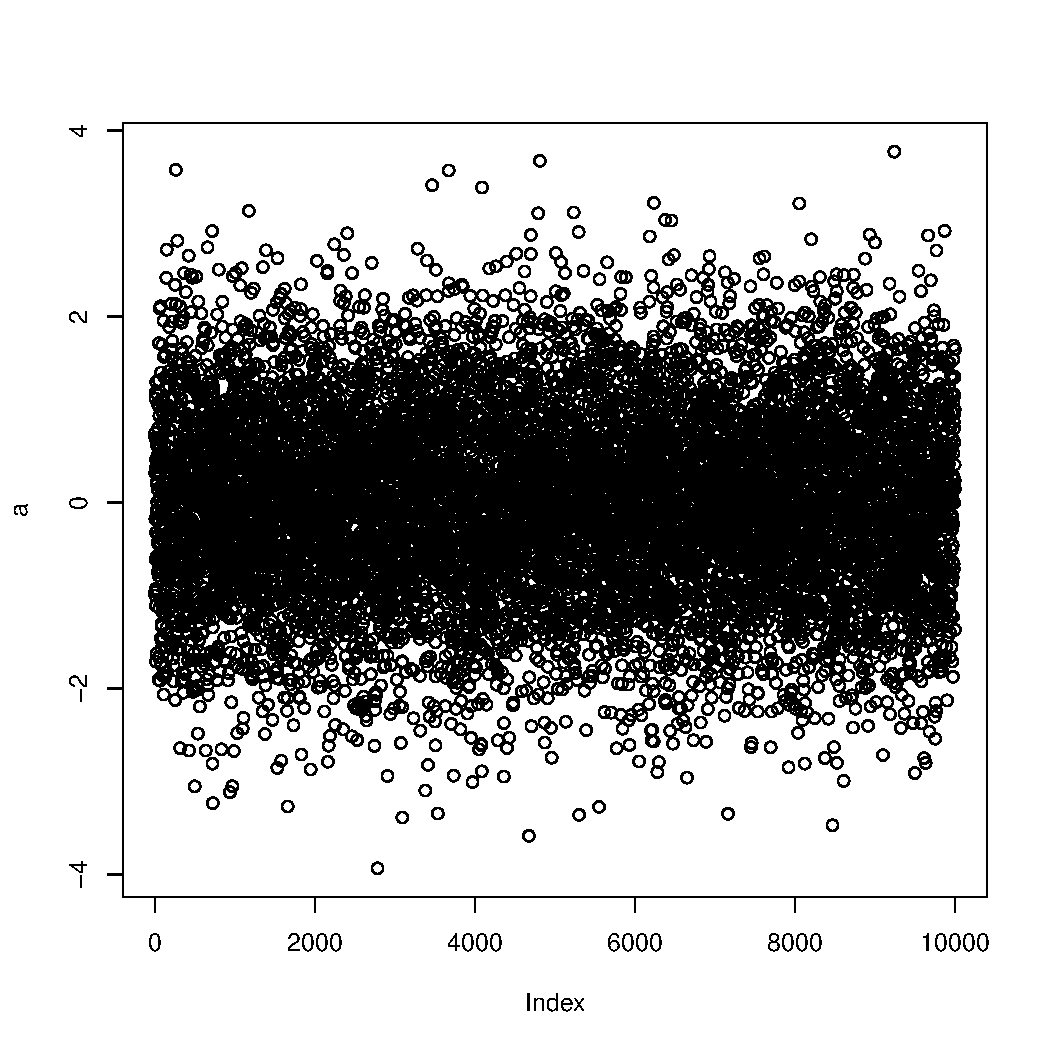
\includegraphics[width=\textwidth]{graphiques/beamer-unnamed-chunk-1-1} } 

}



\end{knitrout}



\begin{knitrout}\footnotesize
\definecolor{shadecolor}{rgb}{0.969, 0.969, 0.969}\color{fgcolor}\begin{kframe}
\begin{alltt}
\hlstd{> }\hlstd{a}\hlkwb{=}\hlkwd{rnorm}\hlstd{(}\hlnum{1000}\hlstd{)}
\hlstd{> }\hlkwd{plot}\hlstd{(a,a}\hlopt{+}\hlkwd{rnorm}\hlstd{(}\hlnum{1000}\hlstd{,}\hlnum{0}\hlstd{,}\hlnum{0.4}\hlstd{))}
\end{alltt}
\end{kframe}

{\centering \resizebox{!}{0.6\textheight}{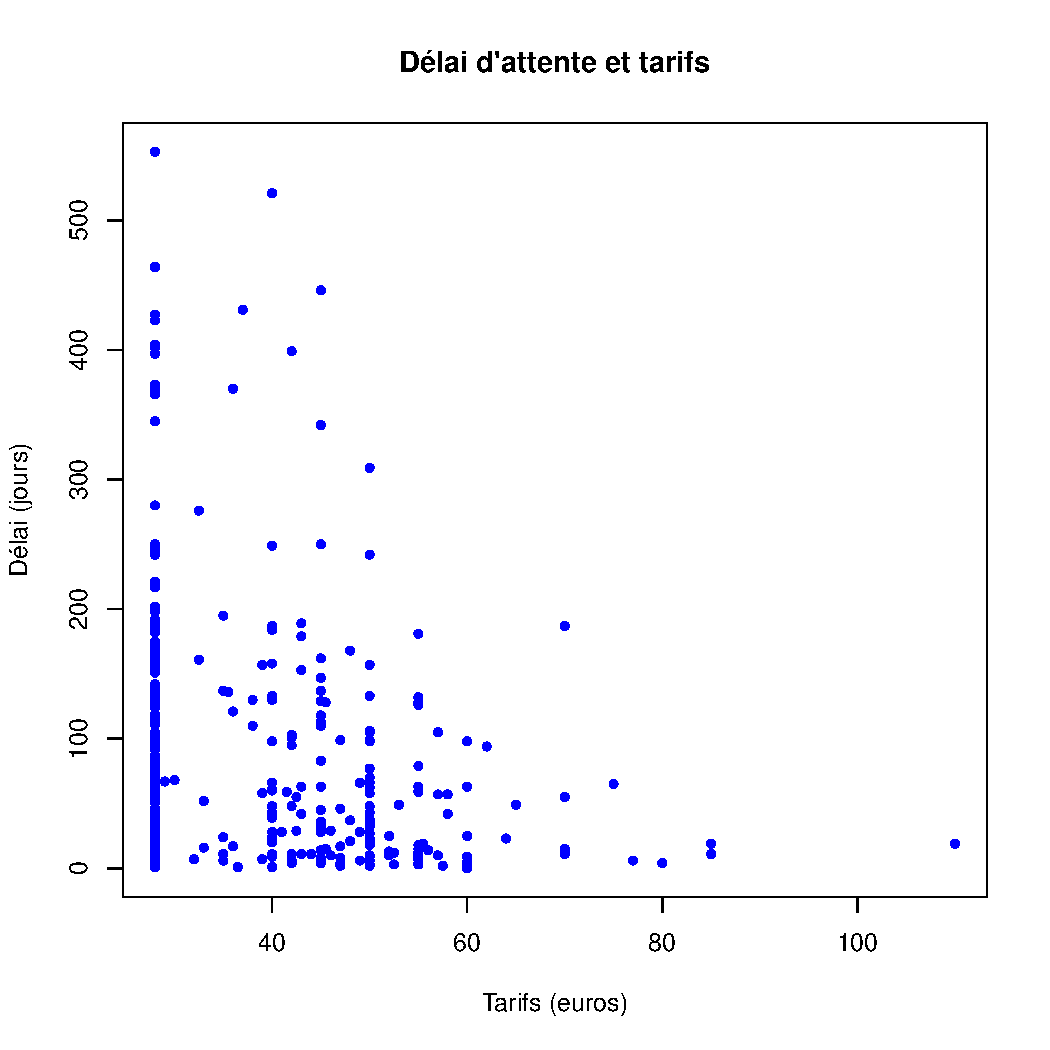
\includegraphics[width=\textwidth]{graphiques/beamer-unnamed-chunk-2-1} } 

}



\end{knitrout}


\begin{knitrout}\footnotesize
\definecolor{shadecolor}{rgb}{0.969, 0.969, 0.969}\color{fgcolor}\begin{kframe}
\begin{alltt}
\hlstd{> }\hlkwd{plot}\hlstd{(}\hlkwd{factor}\hlstd{(}\hlkwd{sample}\hlstd{(LETTERS[}\hlnum{1}\hlopt{:}\hlnum{4}\hlstd{],}\hlnum{1000}\hlstd{,}\hlkwc{replace}\hlstd{=T)),}
\hlstd{+ }            \hlkwd{rnorm}\hlstd{(}\hlnum{1000}\hlstd{)}
\hlstd{+ }            \hlstd{)}
\end{alltt}
\end{kframe}

{\centering \resizebox{!}{0.6\textheight}{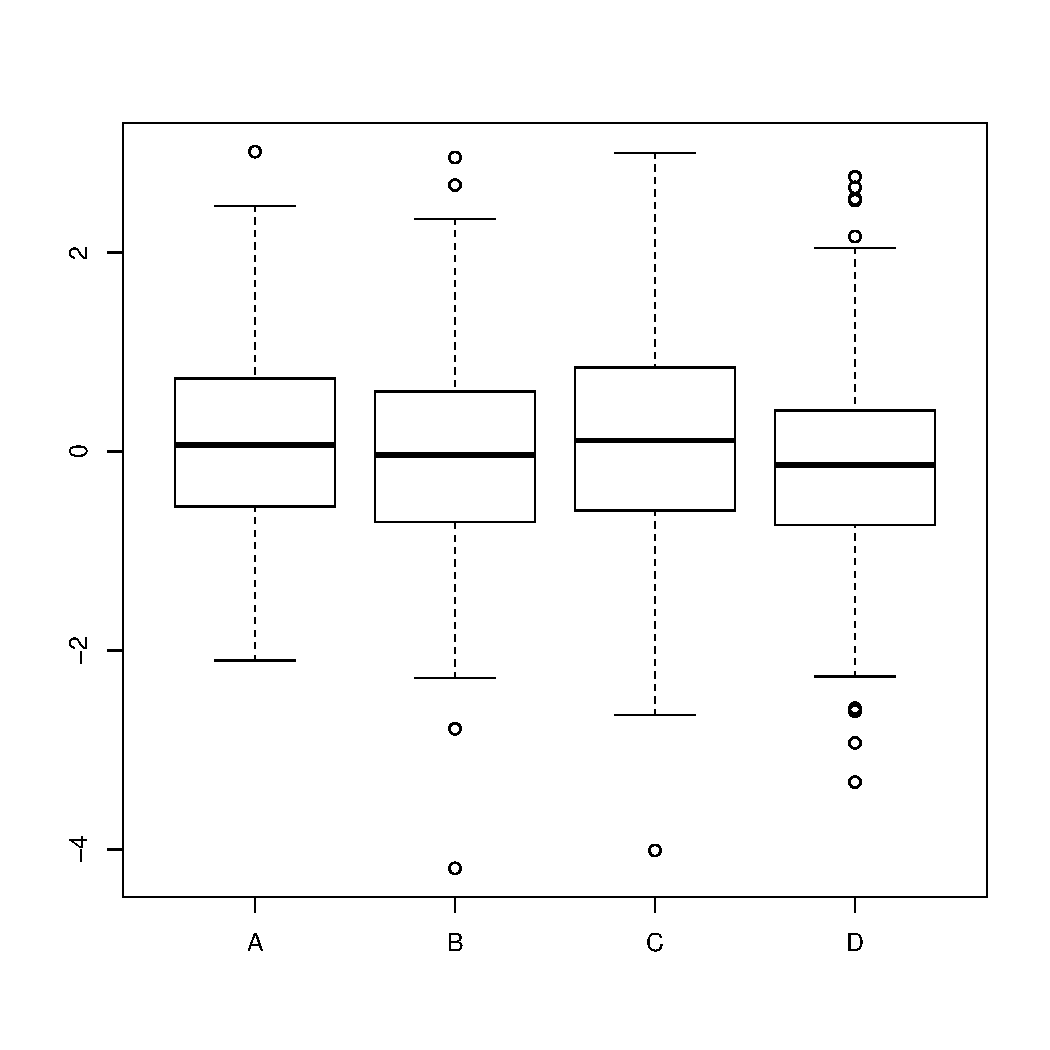
\includegraphics[width=\textwidth]{graphiques/beamer-unnamed-chunk-3-1} } 

}



\end{knitrout}



  
  De nombreux packages utilisent la fonction \emph{plot} pour produire des 
  graphiques en passant un argument propre au paquet.
  
  C'est le cas par exemple pour une r�gression lin�aire dans le paquet de base.
\begin{knitrout}\footnotesize
\definecolor{shadecolor}{rgb}{0.969, 0.969, 0.969}\color{fgcolor}\begin{kframe}
\begin{alltt}
\hlstd{> }\hlstd{a} \hlkwb{<-} \hlkwd{rnorm}\hlstd{(}\hlnum{1000}\hlstd{)}
\hlstd{> }\hlstd{dt} \hlkwb{<-} \hlkwd{data.frame}\hlstd{(}
\hlstd{+ }  \hlkwc{a}\hlstd{=a,}
\hlstd{+ }  \hlkwc{b}\hlstd{=a}\hlopt{+}\hlkwd{rnorm}\hlstd{(}\hlnum{1000}\hlstd{,}\hlnum{0}\hlstd{,}\hlnum{0.4}\hlstd{)}
\hlstd{+ }\hlstd{)}
\hlstd{> }\hlstd{rl} \hlkwb{<-} \hlkwd{lm}\hlstd{(b} \hlopt{~} \hlstd{a)}
\hlstd{> }\hlkwd{plot}\hlstd{(rl,}\hlkwc{ask}\hlstd{=F)}
\end{alltt}
\end{kframe}
\end{knitrout}


  
\begin{knitrout}\footnotesize
\definecolor{shadecolor}{rgb}{0.969, 0.969, 0.969}\color{fgcolor}\begin{kframe}


{\ttfamily\noindent\bfseries\color{errorcolor}{\#\# Error in eval(expr, envir, enclos): objet 'b' introuvable}}\end{kframe}
\end{knitrout}

\begin{knitrout}\footnotesize
\definecolor{shadecolor}{rgb}{0.969, 0.969, 0.969}\color{fgcolor}\begin{kframe}
\begin{alltt}
\hlstd{> }\hlkwd{class}\hlstd{(rl)}
\end{alltt}


{\ttfamily\noindent\bfseries\color{errorcolor}{\#\# Error in eval(expr, envir, enclos): objet 'rl' introuvable}}\end{kframe}
\end{knitrout}

La fonction \emph{plot} est une fonction g�n�rique. En fait la fonction sp�cialis�
pour les objets de type \emph{lm} est appel� en lieu et place de la fonction
usuelle.



  
\begin{knitrout}\footnotesize
\definecolor{shadecolor}{rgb}{0.969, 0.969, 0.969}\color{fgcolor}\begin{kframe}
\begin{alltt}
\hlstd{> }\hlkwd{methods}\hlstd{(}\hlkwc{class}\hlstd{=}\hlkwd{class}\hlstd{(rl))}
\end{alltt}


{\ttfamily\noindent\bfseries\color{errorcolor}{\#\# Error in methods(class = class(rl)): objet 'rl' introuvable}}\end{kframe}
\end{knitrout}

Cette commande est tr�s pratique pour conna�tre les fonctions impl�ment�es pour
ce type d'objet. 


  
  C'est en partie la raison pour laquelle on dit que R est un langage objet car
  c'est un langage dont certaines fonctions sont polymorphiques.
  
  En fait on parle dans ce cas de mod�le S3. Le mod�le S4 qui est plus proche 
  d'un vrai langage objet est peu utilis� pour l'instant.
  

  
  Dans le cas des fonctions graphiques de base, les coordonn�es sont calcul�s
  lors du premi�re appel � la fonction.
  
  Ensuite on peut rajouter des points ou des surfaces et les coordonn�es sont 
  exprim�es dans les m�mes unit�s que celles des donn�es.
  
  Ce n'est pas le cas pour le paquet grid ce qui rend les manipulations
  plus complexes.
  


  \subsection{Les arguments les plus fr�quents}
  
  Les fonctions de base accepte des arguments par d�faut tr�s souvent les m�mes~:
  \begin{description}
    \item[xlim] un vecteur contenant le minimum et le maximum pour l'axe des 
    abscisses
  \item[ylim] un vecteur contenant le minimum et le maximum pour l'axe des 
    ordonn�es
  \item[main] le titre du graphique
  \item[xlab] le nom de l'axe des abscisses
  \item[ylab] le nom de l'axe des ordonn�es
  \item[col] la couleur des poiunts ou des surfaces
\end{description}


  
  Le nombre de param�tres graphiques est impressionnant et il varie malheureusement
  un peu selon les fonctions.
  
  on peut les visualiser avec la commande \emph{par()}.
  
  

  
  Par exemple on peut r�duire les marges~:

\begin{knitrout}\footnotesize
\definecolor{shadecolor}{rgb}{0.969, 0.969, 0.969}\color{fgcolor}\begin{kframe}
\begin{alltt}
\hlstd{> }\hlkwd{par}\hlstd{()}\hlopt{$}\hlstd{mar}
\end{alltt}
\begin{verbatim}
## [1] 5.1 4.1 4.1 2.1
\end{verbatim}
\begin{alltt}
\hlstd{> }\hlkwd{par}\hlstd{(}\hlkwc{mar}\hlstd{=}\hlkwd{c}\hlstd{(}\hlnum{3.1}\hlstd{,}\hlnum{2.1}\hlstd{,}\hlnum{2.1}\hlstd{,}\hlnum{2.1}\hlstd{))}
\hlstd{> }\hlkwd{plot}\hlstd{(dt}\hlopt{$}\hlstd{b,dt}\hlopt{$}\hlstd{a)}
\end{alltt}
\end{kframe}

{\centering \resizebox{!}{0.6\textheight}{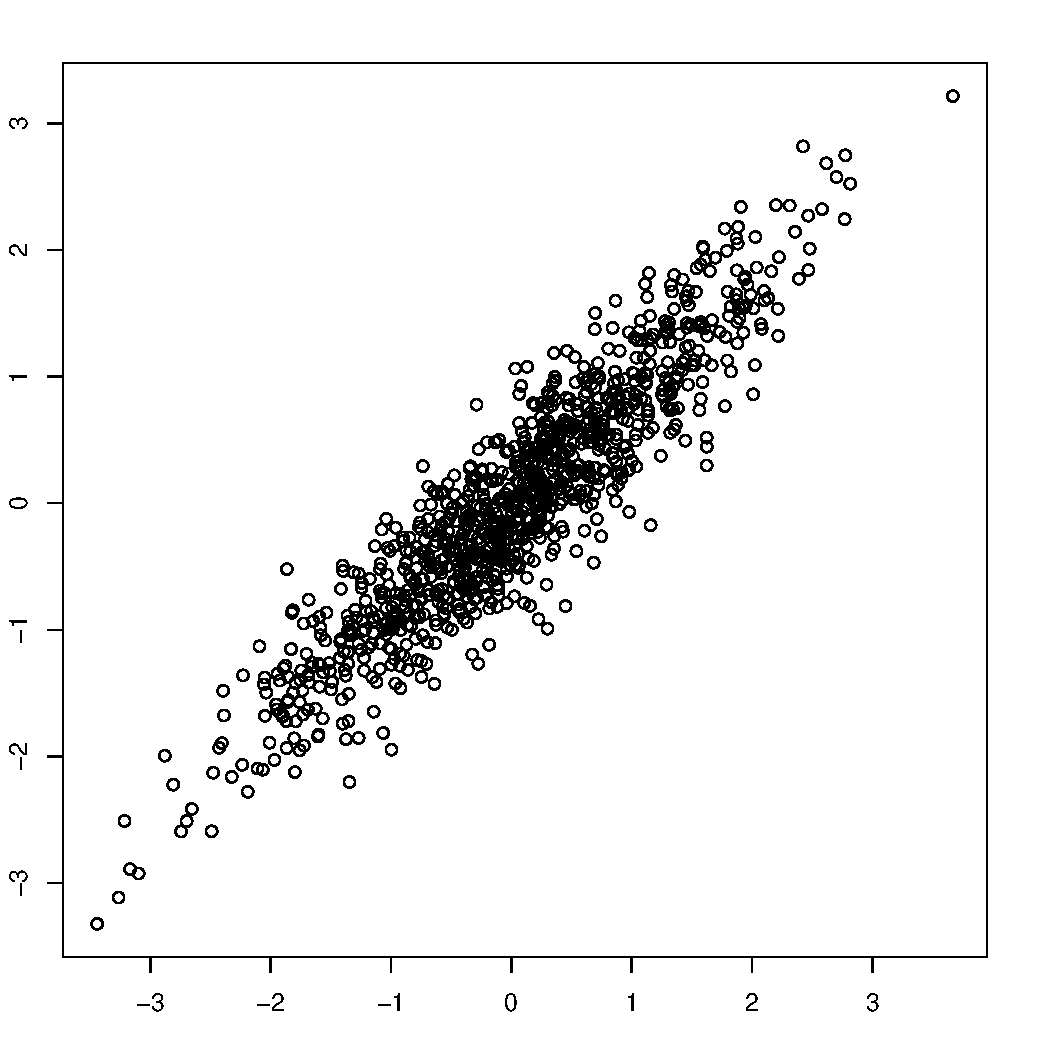
\includegraphics[width=\textwidth]{graphiques/beamer-unnamed-chunk-8-1} } 

}



\end{knitrout}
  
  
  
  On peut �galement faire plusieurs graphiques sur la m�me page~:

\begin{knitrout}\footnotesize
\definecolor{shadecolor}{rgb}{0.969, 0.969, 0.969}\color{fgcolor}\begin{kframe}
\begin{alltt}
\hlstd{> }\hlkwd{par}\hlstd{(}\hlkwc{mfrow}\hlstd{=}\hlkwd{c}\hlstd{(}\hlnum{2}\hlstd{,}\hlnum{2}\hlstd{))}
\hlstd{> }\hlkwd{par}\hlstd{(}\hlkwc{mar}\hlstd{=}\hlkwd{c}\hlstd{(}\hlnum{3.1}\hlstd{,}\hlnum{2.1}\hlstd{,}\hlnum{2.1}\hlstd{,}\hlnum{2.1}\hlstd{))}
\hlstd{> }\hlkwd{plot}\hlstd{(dt}\hlopt{$}\hlstd{b,dt}\hlopt{$}\hlstd{a,}\hlkwc{col}\hlstd{=}\hlstr{"blue"}\hlstd{,}\hlkwc{pch}\hlstd{=}\hlnum{20}\hlstd{)}
\hlstd{> }\hlkwd{plot}\hlstd{(dt}\hlopt{$}\hlstd{b,dt}\hlopt{$}\hlstd{a,}\hlkwc{col}\hlstd{=}\hlstr{"green"}\hlstd{,}\hlkwc{pch}\hlstd{=}\hlnum{20}\hlstd{)}
\hlstd{> }\hlkwd{plot}\hlstd{(dt}\hlopt{$}\hlstd{b,dt}\hlopt{$}\hlstd{a,}\hlkwc{col}\hlstd{=}\hlstr{"yellow"}\hlstd{,}\hlkwc{pch}\hlstd{=}\hlnum{20}\hlstd{)}
\hlstd{> }\hlkwd{plot}\hlstd{(dt}\hlopt{$}\hlstd{b,dt}\hlopt{$}\hlstd{a,}\hlkwc{col}\hlstd{=}\hlstr{"red"}\hlstd{,}\hlkwc{pch}\hlstd{=}\hlnum{20}\hlstd{)}
\end{alltt}
\end{kframe}
\end{knitrout}
  


  
  On peut �galement faire plusieurs graphiques sur la m�me page~:

\begin{knitrout}\footnotesize
\definecolor{shadecolor}{rgb}{0.969, 0.969, 0.969}\color{fgcolor}

{\centering \resizebox{!}{0.6\textheight}{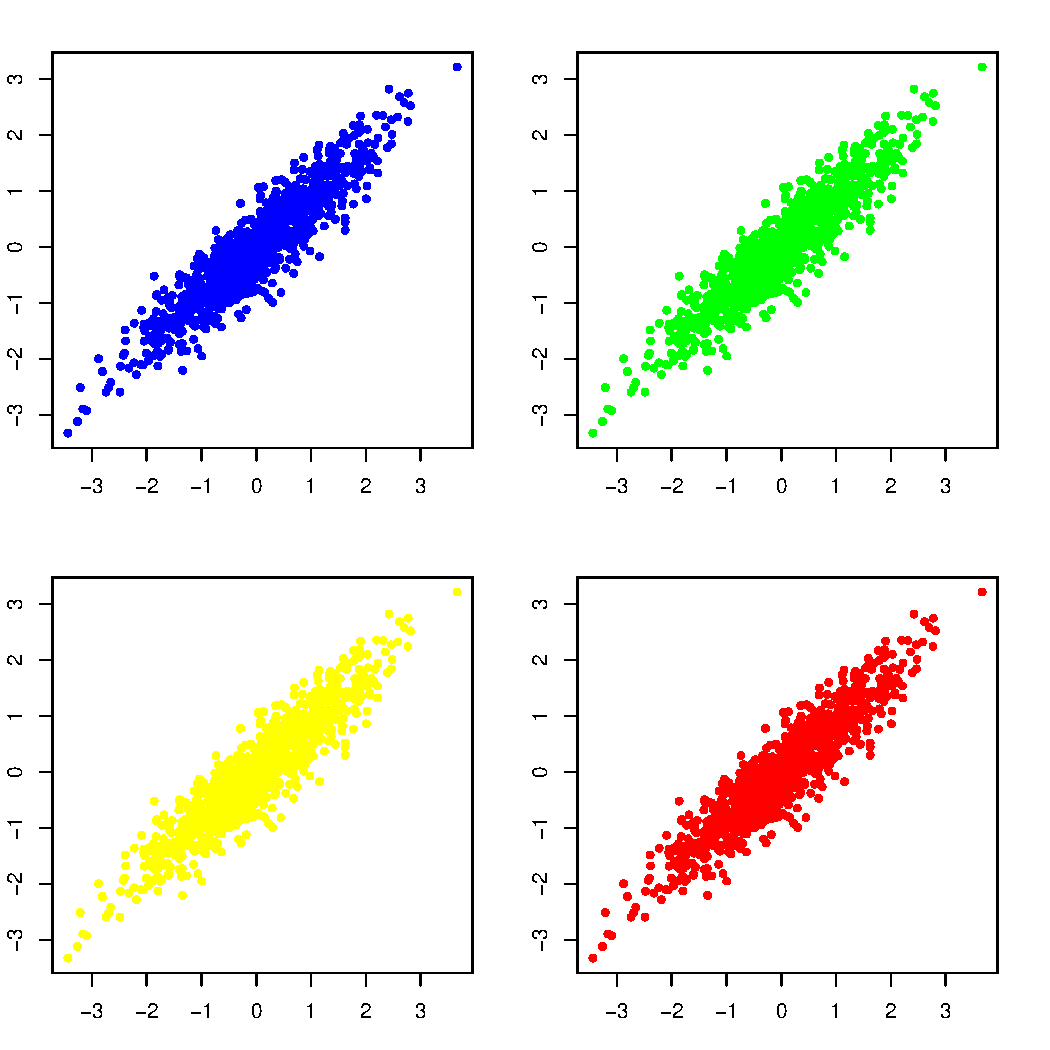
\includegraphics[width=\textwidth]{graphiques/beamer-unnamed-chunk-10-1} } 

}



\end{knitrout}
  

  
  
\begin{knitrout}\footnotesize
\definecolor{shadecolor}{rgb}{0.969, 0.969, 0.969}\color{fgcolor}

{\centering \resizebox{!}{0.6\textheight}{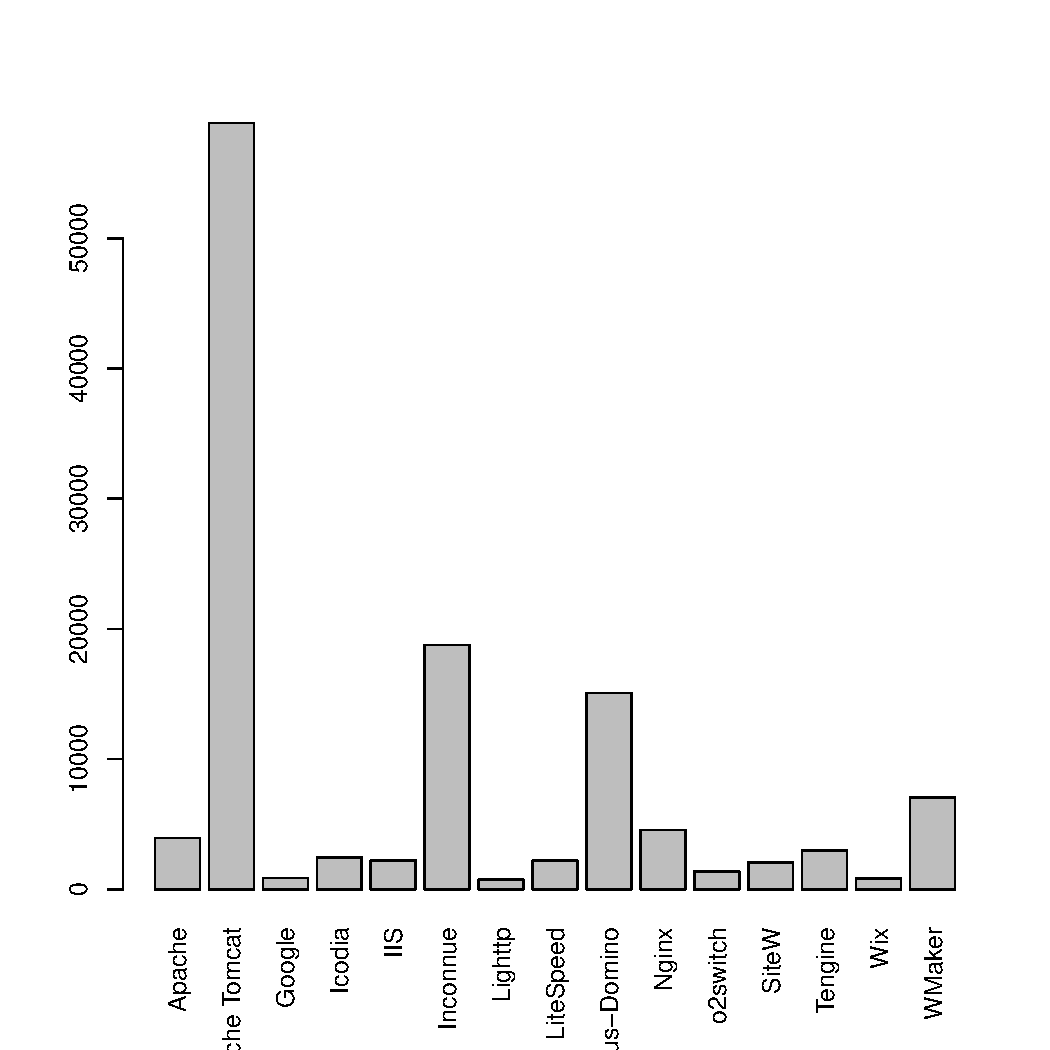
\includegraphics[width=\textwidth]{graphiques/beamer-unnamed-chunk-11-1} } 

}



\end{knitrout}
  


  \subsection{Les fonctions de superposition}

  Il faut distinguer deux types de fonctions~:
  \begin{itemize}
    \item les fonctions d'initialisation et de trac�
    \item les fonctions de superpositions sur un trac�
  \end{itemize}
  
  Un graphique R de base n'existe pas comme dit plus sans une �chelle des X
  et une �chelle des Y. Les fonctions comme \emph{plot}, \emph{barplot}, 
  \emph{hist}, \dots initialise le graphique et font tout ce qu'il faut 
  pour tracer un graphique.




  Les fonctions de superposition permettent de r�aliser des trac�s mais en utilisant
  sur des graphiques existants.
  
  Soit il s'agit de fonctions distinctes~:
  \begin{itemize}
    \item \emph{lines}
    \item \emph{points}
    \item \emph{text}
    \item \dots
  \end{itemize}
  


  Les fonctions de superposition permettent de r�aliser des trac�s mais en utilisant
  sur des graphiques existants.
  
  Soit il s'agit de fonctions d'initialisation mais avec un argument sp�cifique~:
  g�n�ralement il s'agit de rajouter l'argument \emph{add}~:
\begin{knitrout}\footnotesize
\definecolor{shadecolor}{rgb}{0.969, 0.969, 0.969}\color{fgcolor}\begin{kframe}
\begin{alltt}
\hlstd{> }\hlkwd{plot}\hlstd{(x,y,}\hlkwc{add}\hlstd{=T)}
\end{alltt}
\end{kframe}
\end{knitrout}


  \subsection{La notion de \emph{device}}
  
  La sortie par d�faut sur R est une fen�tre graphique. Par exemple dans RStudio
  l'onglet plot en bas � droite.
  
  Mais on peut cr�er des graphiques dans des devices diff�rents tels que des fichiers.
  Par exemple pour cr�er un fichier jpeg, il faut ouvrir un device \emph{jpeg} qui
  va se substituer � la fen�tre graphique. Puis on va fermer le device pour finaliser
  l'export.


\section{Les devices}


  
\begin{knitrout}\footnotesize
\definecolor{shadecolor}{rgb}{0.969, 0.969, 0.969}\color{fgcolor}\begin{kframe}
\begin{alltt}
\hlstd{> }\hlkwd{jpeg}\hlstd{(}\hlstr{"graphiques/MonGraphique.jpeg"}\hlstd{)}
\hlstd{> }\hlkwd{par}\hlstd{(}\hlkwc{mfrow}\hlstd{=}\hlkwd{c}\hlstd{(}\hlnum{2}\hlstd{,}\hlnum{2}\hlstd{))}
\hlstd{> }\hlkwd{par}\hlstd{(}\hlkwc{mar}\hlstd{=}\hlkwd{c}\hlstd{(}\hlnum{3.1}\hlstd{,}\hlnum{2.1}\hlstd{,}\hlnum{2.1}\hlstd{,}\hlnum{2.1}\hlstd{))}
\hlstd{> }\hlkwd{plot}\hlstd{(dt}\hlopt{$}\hlstd{b,dt}\hlopt{$}\hlstd{a,}\hlkwc{col}\hlstd{=}\hlstr{"blue"}\hlstd{,}\hlkwc{pch}\hlstd{=}\hlnum{20}\hlstd{)}
\hlstd{> }\hlkwd{plot}\hlstd{(dt}\hlopt{$}\hlstd{b,dt}\hlopt{$}\hlstd{a,}\hlkwc{col}\hlstd{=}\hlstr{"green"}\hlstd{,}\hlkwc{pch}\hlstd{=}\hlnum{20}\hlstd{)}
\hlstd{> }\hlkwd{plot}\hlstd{(dt}\hlopt{$}\hlstd{b,dt}\hlopt{$}\hlstd{a,}\hlkwc{col}\hlstd{=}\hlstr{"yellow"}\hlstd{,}\hlkwc{pch}\hlstd{=}\hlnum{20}\hlstd{)}
\hlstd{> }\hlkwd{plot}\hlstd{(dt}\hlopt{$}\hlstd{b,dt}\hlopt{$}\hlstd{a,}\hlkwc{col}\hlstd{=}\hlstr{"red"}\hlstd{,}\hlkwc{pch}\hlstd{=}\hlnum{20}\hlstd{)}
\hlstd{> }\hlkwd{dev.off}\hlstd{()}
\end{alltt}
\begin{verbatim}
## pdf 
##   2
\end{verbatim}
\end{kframe}
\end{knitrout}



  Les formats sont nombreux~:
  \begin{itemize}
    \item png
    \item pdf
    \item svg
    \item \dots
  \end{itemize}
  
  Chaque device porte le nom du type de fichier qu'il va cr��.
  

  
  \subsection{La proc�dure avec les \emph{device}}

  La proc�dure se fait avec les �tapes suivantes~:
  \begin{enumerate}
      \item vous cr�ez le device avec par exemple \emph{png("file")}
      \item vous dessinez
      \item vous refermez le device avec la commande \emph{dev.off()}
  \end{enumerate}
  
  Quelque devices comme le pdf permet de produire plusieurs graphiques sur
  plusieurs pages comme par exemple le format PDF.
  

  \subsection{Les arguments des \emph{device}}
  
  Les arguments varient, il suffit de regarder l'aide. Souvent on trouve
  l'argument dpi qui permet de donner la r�solution du graphique.
  
  Les arguments width et height donnent la taille dont l'unit� d�pend du device
  choisi.



  \subsection{Les options d'agencement avanc�e}
  
  L'option \emph{layout} permet de d�finir des agencements avanc�s comme sur le 
  graphique ci-dessous.
  
  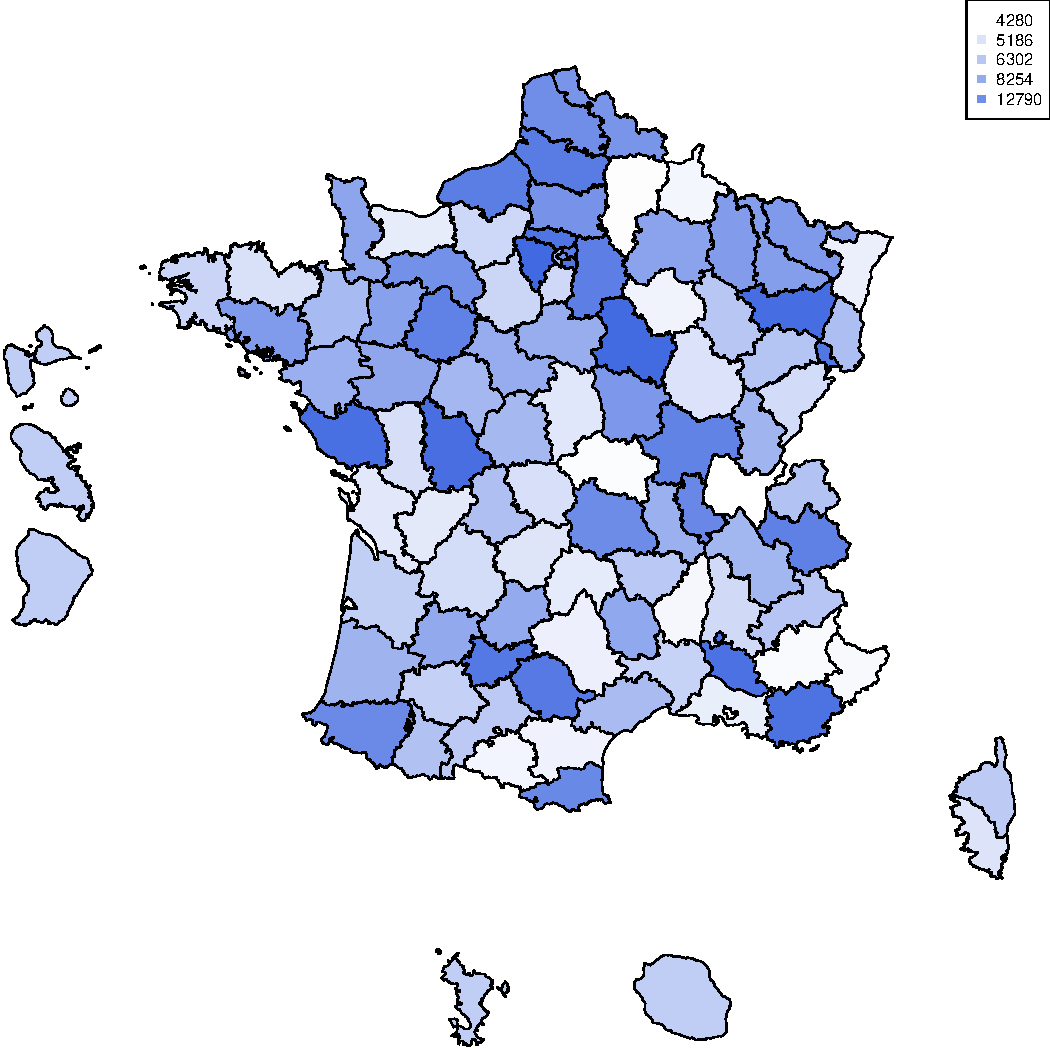
\includegraphics[scale=0.4]{graphiques/cartes_pleines}



  
  Il suffit de donner en entr�e une matrice avec un num�ro dans l'ordre de ce qui 
  va �tre dessiner. Les fusions des cellules de la matrice donnent la taille
  de chaque zone.

  Dans l'exemple, on repr�sente un grand graphique central pour la France
  m�tropolitaine puis des petits carr�s pour les DOMs.



  
  Il suffit de donner en entr�e une matrice avec un num�ro dans l'ordre de ce qui 
  va �tre dessiner. Les fusions des cellules de la matrice donnent la taille
  de chaque zone.

  Dans l'exemple, on repr�sente un grand graphique central pour la France
  m�tropolitaine puis des petits carr�s pour les DOMs.




\begin{knitrout}\footnotesize
\definecolor{shadecolor}{rgb}{0.969, 0.969, 0.969}\color{fgcolor}\begin{kframe}
\begin{alltt}
\hlstd{> }\hlstd{xmetro} \hlkwb{<-} \hlnum{9}
\hlstd{> }\hlstd{xdom} \hlkwb{<-} \hlnum{1}
\hlstd{> }\hlstd{mm} \hlkwb{<-} \hlkwd{matrix}\hlstd{(}
\hlstd{+ }    \hlkwd{c}\hlstd{(}
\hlstd{+ }      \hlkwd{rep}\hlstd{(} \hlnum{7}\hlstd{,xdom),} \hlkwd{rep}\hlstd{(} \hlnum{1}\hlstd{,xmetro),}
\hlstd{+ }      \hlkwd{rep}\hlstd{(} \hlnum{7}\hlstd{,xdom),} \hlkwd{rep}\hlstd{(} \hlnum{1}\hlstd{,xmetro),}
\hlstd{+ }      \hlkwd{rep}\hlstd{(} \hlnum{7}\hlstd{,xdom),} \hlkwd{rep}\hlstd{(} \hlnum{1}\hlstd{,xmetro),}
\hlstd{+ }      \hlkwd{rep}\hlstd{(} \hlnum{2}\hlstd{,xdom),} \hlkwd{rep}\hlstd{(} \hlnum{1}\hlstd{,xmetro),}
\hlstd{+ }      \hlkwd{rep}\hlstd{(} \hlnum{3}\hlstd{,xdom),} \hlkwd{rep}\hlstd{(} \hlnum{1}\hlstd{,xmetro),}
\hlstd{+ }      \hlkwd{rep}\hlstd{(} \hlnum{4}\hlstd{,xdom),} \hlkwd{rep}\hlstd{(} \hlnum{1}\hlstd{,xmetro),}
\hlstd{+ }      \hlkwd{rep}\hlstd{(} \hlnum{0}\hlstd{,xdom),} \hlkwd{rep}\hlstd{(} \hlnum{1}\hlstd{,xmetro),}
\hlstd{+ }      \hlkwd{rep}\hlstd{(} \hlnum{0}\hlstd{,xdom),} \hlkwd{rep}\hlstd{(} \hlnum{1}\hlstd{,xmetro),}
\hlstd{+ }      \hlkwd{rep}\hlstd{(} \hlnum{0}\hlstd{,xdom),} \hlkwd{rep}\hlstd{(} \hlnum{1}\hlstd{,xmetro),}
\hlstd{+ }      \hlkwd{rep}\hlstd{(} \hlnum{0}\hlstd{,xdom),} \hlkwd{rep}\hlstd{(}\hlnum{0}\hlstd{,}\hlnum{3}\hlstd{),} \hlkwd{rep}\hlstd{(}\hlnum{5}\hlstd{,}\hlnum{1}\hlstd{),} \hlkwd{rep}\hlstd{(}\hlnum{0}\hlstd{,}\hlnum{1}\hlstd{),} \hlkwd{rep}\hlstd{(}\hlnum{6}\hlstd{,}\hlnum{1}\hlstd{),} \hlkwd{rep}\hlstd{(}\hlnum{0}\hlstd{,xmetro}\hlopt{-}\hlnum{6}\hlstd{)}
\hlstd{+ }    \hlstd{),}
\hlstd{+ }    \hlkwc{ncol}\hlstd{=}\hlnum{10}\hlstd{,}
\hlstd{+ }    \hlkwc{nrow}\hlstd{=}\hlnum{10}\hlstd{,}
\hlstd{+ }    \hlkwc{byrow}\hlstd{=T}
\hlstd{+ }\hlstd{)}
\hlstd{> }\hlstd{mm}
\end{alltt}
\end{kframe}
\end{knitrout}



\begin{knitrout}\footnotesize
\definecolor{shadecolor}{rgb}{0.969, 0.969, 0.969}\color{fgcolor}\begin{kframe}
\begin{verbatim}
##       [,1] [,2] [,3] [,4] [,5] [,6] [,7]
##  [1,]    7    1    1    1    1    1    1
##  [2,]    7    1    1    1    1    1    1
##  [3,]    7    1    1    1    1    1    1
##  [4,]    2    1    1    1    1    1    1
##  [5,]    3    1    1    1    1    1    1
##  [6,]    4    1    1    1    1    1    1
##  [7,]    0    1    1    1    1    1    1
##  [8,]    0    1    1    1    1    1    1
##  [9,]    0    1    1    1    1    1    1
## [10,]    0    0    0    0    5    0    6
##       [,8] [,9] [,10]
##  [1,]    1    1     1
##  [2,]    1    1     1
##  [3,]    1    1     1
##  [4,]    1    1     1
##  [5,]    1    1     1
##  [6,]    1    1     1
##  [7,]    1    1     1
##  [8,]    1    1     1
##  [9,]    1    1     1
## [10,]    0    0     0
\end{verbatim}
\end{kframe}
\end{knitrout}




\documentclass{beamer}\usepackage[]{graphicx}\usepackage[]{color}
%% maxwidth is the original width if it is less than linewidth
%% otherwise use linewidth (to make sure the graphics do not exceed the margin)
\makeatletter
\def\maxwidth{ %
  \ifdim\Gin@nat@width>\linewidth
    \linewidth
  \else
    \Gin@nat@width
  \fi
}
\makeatother

\definecolor{fgcolor}{rgb}{0.345, 0.345, 0.345}
\newcommand{\hlnum}[1]{\textcolor[rgb]{0.686,0.059,0.569}{#1}}%
\newcommand{\hlstr}[1]{\textcolor[rgb]{0.192,0.494,0.8}{#1}}%
\newcommand{\hlcom}[1]{\textcolor[rgb]{0.678,0.584,0.686}{\textit{#1}}}%
\newcommand{\hlopt}[1]{\textcolor[rgb]{0,0,0}{#1}}%
\newcommand{\hlstd}[1]{\textcolor[rgb]{0.345,0.345,0.345}{#1}}%
\newcommand{\hlkwa}[1]{\textcolor[rgb]{0.161,0.373,0.58}{\textbf{#1}}}%
\newcommand{\hlkwb}[1]{\textcolor[rgb]{0.69,0.353,0.396}{#1}}%
\newcommand{\hlkwc}[1]{\textcolor[rgb]{0.333,0.667,0.333}{#1}}%
\newcommand{\hlkwd}[1]{\textcolor[rgb]{0.737,0.353,0.396}{\textbf{#1}}}%

\usepackage{framed}
\makeatletter
\newenvironment{kframe}{%
 \def\at@end@of@kframe{}%
 \ifinner\ifhmode%
  \def\at@end@of@kframe{\end{minipage}}%
  \begin{minipage}{\columnwidth}%
 \fi\fi%
 \def\FrameCommand##1{\hskip\@totalleftmargin \hskip-\fboxsep
 \colorbox{shadecolor}{##1}\hskip-\fboxsep
     % There is no \\@totalrightmargin, so:
     \hskip-\linewidth \hskip-\@totalleftmargin \hskip\columnwidth}%
 \MakeFramed {\advance\hsize-\width
   \@totalleftmargin\z@ \linewidth\hsize
   \@setminipage}}%
 {\par\unskip\endMakeFramed%
 \at@end@of@kframe}
\makeatother

\definecolor{shadecolor}{rgb}{.97, .97, .97}
\definecolor{messagecolor}{rgb}{0, 0, 0}
\definecolor{warningcolor}{rgb}{1, 0, 1}
\definecolor{errorcolor}{rgb}{1, 0, 0}
\newenvironment{knitrout}{}{} % an empty environment to be redefined in TeX

\usepackage{alltt}
\usetheme[compress]{Singapore}
\useoutertheme{miniframes}

% \documentclass{beamer}
%\usetheme{Warsaw}

% Pour les documents en francais...
	\usepackage[latin1]{inputenc}
	\usepackage[french]{babel}
	\usepackage[french]{varioref}

% Math�matiques
	\usepackage{amsmath}

% Caracteres speciaux suppl�mentaires
	\usepackage{latexsym,amsfonts}

% A documenter
	\usepackage{moreverb}

% Macros pour les paquets
	\usepackage{array}  			% N�cessaires pour les tableaux de la macro Excel.

% Outil suppl�mentaire pour les tableaux
	\usepackage{multirow}
	\usepackage{booktabs}
	\usepackage{xcolor} % alternating row colors in table, incompatible avec certains modules
	\usepackage{longtable}
	\usepackage{colortbl}

% Pour ins�rer des graphiques
	\usepackage{graphicx} 			% Graphique simples
	\usepackage{subfigure}			% Graphiques multiples

% Pour ins�rer des couleurs
	\usepackage{color}

% Rotation des objets et des pages
%	\usepackage{rotating}
%	\usepackage{lscape}

% Pour insrer du code source, LaTeX ou SAS par exemple.
	\usepackage{verbatim}
  \usepackage{moreverb}
	\usepackage{listings}
	\usepackage{fancyvrb}

%	\lstset{language=SAS,numbers=left}		% Par dfaut le listing est en SAS
\lstset{breaklines=true}  % marche pas

% Pour ins�rer des hyperliens
  \usepackage{hyperref}

% American Psychological Association (for bibliographic references).
	\usepackage{apacite}

% Pour l'utilisation des macros
	\usepackage{xspace}

% Pour l'utilisation de notes en fin de document.
%	\usepackage{endnotes}

% Array
%	\usepackage{multirow}
%	\usepackage{booktabs}

% Rotation
%	\usepackage{rotating}

% En t�tes et pieds de pages
%	\usepackage{fancyhdr}
%	\usepackage{lastpage}


% Page layout

% By LaTeX commands
%\setlength{\oddsidemargin}{0cm}
%\setlength{\textwidth}{16cm}
%\setlength{\textheight}{24cm}
%\setlength{\topmargin}{-1cm}
%\setlength{\marginparsep}{0.2cm}

% fancyheader parameters
%\pagestyle{fancy}

%\fancyfoot[L]{{\small Formation \LaTeX, DEPP}}
%\fancyfoot[c]{}
%\fancyfoot[R]{{\small \thepage/\pageref{LastPage}}}

%\fancyhead[L]{}
%\fancyhead[c]{}
%\fancyhead[R]{}

% Pour ins�rer des dessins de Linux
\newcommand{\LinuxA}{\includegraphics[height=0.5cm]{Graphiques/linux.png}}
\newcommand{\LinuxB}{\includegraphics[height=0.5cm]{Graphiques/linux.png}\xspace}

% Macro pour les petits dessins pour les diff�rents OS.
\newcommand{\Windows}{\emph{Windows}\xspace}
\newcommand{\Mac}{\emph{Mac OS X}\xspace}
\newcommand{\Linux}{\emph{Linux}\xspace}
\newcommand{\MikTeX}{MiK\tex\xspace}

\newcommand{\df}{\emph{data.frame}\xspace}
\newcommand{\dfs}{\emph{data.frames}\xspace}


\newcommand{\liste}{\emph{list}\xspace}
\newcommand{\factor}{\emph{factor}\xspace}
\newcommand{\character}{\emph{character}\xspace}
\newcommand{\logical}{\emph{logical}\xspace}

\newcommand{\cad}{c'est-�-dire\xspace}

\newcommand{\hreff}[2]{\underline{\href{#1}{#2}\xspace}}


% Titre
\title{Introduction � R}
\author{Pascal Bessonneau}
%\institute{DEPP}
\date{06/2015}

\subtitle{Manipulations de donn�es}




\IfFileExists{upquote.sty}{\usepackage{upquote}}{}
\begin{document}

\begin{frame}
	\maketitle
\end{frame}

\begin{frame}
	\tableofcontents
\end{frame}

% Begin document %%%%%%%%%%%%%%%%%%%%%%%%%%%%%%%%%%%%%%%%%%%%%%%%%%%%%%%%%%%%%%%%%%%%%%%%%%%%%%%%%%

\section{Concat�nation de donn�es (merge)}

\begin{frame}[containsverbatim]
  \frametitle{A ne pas faire (ou avec prudence)}
  
  R permet de concat�ner des lignes (\textit{rbind}), des colonnes (\textit{cbind}), des \dfs (m�mes fonctions) ensemble. Toutefois il convient d'utiliser avec sagesse cette fonctionnalit�.
  
  Si en sciences exp�rimentales faire une fusion de table avec une simple concat�nation est tr�s pratique, cette op�ration n'est pas raisonnable sur des tables plus complexes et surtout sur des tables contenant des identifiants qui permettent de r�aliser une fusion plut�t qu'une concat�nation.
    
\end{frame}

\begin{frame}[containsverbatim]
  \frametitle{A ne pas faire (ou avec prudence)}

  En tout cas d�s que \textit{cbind} est utilis� il faut v�rifier~: 
     \begin{itemize}
       \item que les deux tableaux ont la m�me taille
       \item chaque ligne identifie une observation 
       \item que les observations sont strictement dans le m�me ordre dans les deux tableaux
     \end{itemize}

\end{frame}

\begin{frame}[containsverbatim]
  \frametitle{A ne pas faire (ou avec prudence)}

  En tout cas d�s que \textit{rbind} est utilis� il faut v�rifier~: 
\begin{itemize}
  \item que le nombre de colonnes sont identiques
   \item que le type de chaque colonnes sont identiques
\end{itemize}

  \textit{rbind} est un peu plus s�r car R g�n�ralement refuse d'op�rer en cas de diff�rence de noms et/ou de types de variables dans les deux tableaux de donn�es.
  
\end{frame}



\begin{frame}[containsverbatim]
  \frametitle{A ne pas faire (ou avec prudence)}

  \textit{rbind} s'av�re quand m�me pratique si on souhaite travailler par exemple sur une base
public et une priv�... et r�assembler le tout � la fin du traitement.

  C'est typiquement le cas par exemple quand on utilise \textit{split}.
  
\end{frame}

\begin{frame}[containsverbatim]
  \frametitle{Fusion avec une seule variable}
  
  Ce cas est en fait beaucoup plus fr�quent qu'il n'y parait. On veux par exemple ajouter une variable avec une couleur pour les graphiques, le nombre d'�l�ves dans l'�tablissement, \dots
  
  Et ce type de fusion se fait avec un vecteur. 
  
\begin{knitrout}\footnotesize
\definecolor{shadecolor}{rgb}{0.969, 0.969, 0.969}\color{fgcolor}\begin{kframe}
\begin{alltt}
\hlstd{> }\hlstd{couleurs} \hlkwb{<-} \hlkwd{c}\hlstd{(} \hlstr{"red"}\hlstd{,} \hlstr{"green"}\hlstd{,} \hlstr{"blue"} \hlstd{)}
\hlstd{> }\hlkwd{names}\hlstd{(couleurs)} \hlkwb{<-} \hlkwd{levels}\hlstd{(iris}\hlopt{$}\hlstd{Species)}
\hlstd{> }\hlstd{iris}\hlopt{$}\hlstd{couleur} \hlkwb{<-} \hlstd{couleurs[}\hlkwd{as.character}\hlstd{(iris}\hlopt{$}\hlstd{Species)]}
\hlstd{> }\hlkwd{with}\hlstd{( iris,} \hlkwd{table}\hlstd{(couleur,Species) )}
\end{alltt}
\begin{verbatim}
##        Species
## couleur setosa versicolor virginica
##   blue       0          0        50
##   green      0         50         0
##   red       50          0         0
\end{verbatim}
\end{kframe}
\end{knitrout}
  
\end{frame}

\begin{frame}[containsverbatim]
  \frametitle{Fusion avec une seule variable}

  Un exemple num�rique, si on veut ajouter la longueur moyenne par esp�ce pour les orchid�es~:
  
\begin{knitrout}\footnotesize
\definecolor{shadecolor}{rgb}{0.969, 0.969, 0.969}\color{fgcolor}\begin{kframe}
\begin{alltt}
\hlstd{> }\hlstd{longueur_par_spe} \hlkwb{<-} \hlkwd{tapply}\hlstd{( iris}\hlopt{$}\hlstd{Sepal.Length, iris}\hlopt{$}\hlstd{Species, mean )}
\hlstd{> }\hlstd{iris}\hlopt{$}\hlstd{Sepal.Length.Moy} \hlkwb{<-} \hlstd{longueur_par_spe[}\hlkwd{as.character}\hlstd{(iris}\hlopt{$}\hlstd{Species)]}
\hlstd{> }\hlkwd{with}\hlstd{( iris,} \hlkwd{table}\hlstd{(Sepal.Length.Moy,Species) )}
\end{alltt}
\begin{verbatim}
##                 Species
## Sepal.Length.Moy setosa versicolor virginica
##            5.006     50          0         0
##            5.936      0         50         0
##            6.588      0          0        50
\end{verbatim}
\end{kframe}
\end{knitrout}
  
\end{frame}


\begin{frame}[containsverbatim]
  \frametitle{Fusions avec merge}

La fonction \emph{merge} dans R permet de fusionner des tables avec un
identifiant (clef) commun entre les tables.

La fusion peut �tre r�alis�e en utilisant des variables \emph{factor}
mais il est pr�f�rable de les transformer variable \emph{character} avant la fusion.

Les fusions possibles sont des fusions de 1 � 1 ou de 1 � n.

\end{frame}

\begin{frame}[containsverbatim]
  \frametitle{Fusions avec merge}

  \begin{table}[h!]
  \scalebox{0.8}{
    \begin{tabular}{lp{10cm}}
  { \bfseries x, y } & les 2 \emph{data.frames} que l'on veut fusionner\\
  { \bfseries by } & si la variable porte le m�me nom dans les deux \emph{data.frame},
  il suffit de pr�ciser le nom de la variable pr�c�d� de \emph{by}\\
  { \bfseries by.x, by.y } & dans ce cas on sp�cifie le nom de la
  colonne pour \emph{x} (la premi�re \emph{data.frame} et pour \emph{y}
  (la deuxi�me).\\
  \end{tabular}
  }
  \caption[position=bottom]{Les principaux arguments de \emph{merge}}
  \end{table}
  
  Voil� l'essentiel de la fonction.

\end{frame}

\begin{frame}[containsverbatim]
  \frametitle{Fusions avec merge}

  Il faut noter qu'on a la possibilit� de fusionner les tables non pas en utilisant le nom d'une variable de la \df mais les \emph{row.names}. Dans ce cas, l'argument que l'on passe � \emph{by}
  est \emph{'row.names'}.

\begin{knitrout}\footnotesize
\definecolor{shadecolor}{rgb}{0.969, 0.969, 0.969}\color{fgcolor}\begin{kframe}
\begin{alltt}
\hlstd{> }\hlstd{res} \hlkwb{<-} \hlkwd{merge}\hlstd{( eleves, scores,} \hlkwc{by}\hlstd{=}\hlstr{"id"} \hlstd{)}
\hlstd{> }\hlkwd{dim}\hlstd{(res)}
\end{alltt}
\begin{verbatim}
## [1] 5000    7
\end{verbatim}
\end{kframe}
\end{knitrout}

\end{frame}

\begin{frame}[containsverbatim]
  \frametitle{Fusions avec merge}

  Dans le cas de l'utilisation des rownames~:

\begin{knitrout}\footnotesize
\definecolor{shadecolor}{rgb}{0.969, 0.969, 0.969}\color{fgcolor}\begin{kframe}
\begin{alltt}
\hlstd{> }\hlkwd{rownames}\hlstd{(eleves)} \hlkwb{<-} \hlstd{eleves}\hlopt{$}\hlstd{id}
\hlstd{> }\hlkwd{rownames}\hlstd{(scores)} \hlkwb{<-} \hlstd{scores}\hlopt{$}\hlstd{id}
\hlstd{> }
\hlstd{> }\hlstd{res} \hlkwb{<-} \hlkwd{merge}\hlstd{( eleves, scores,} \hlkwc{by}\hlstd{=}\hlstr{"row.names"} \hlstd{)}
\hlstd{> }\hlkwd{dim}\hlstd{(res)}
\end{alltt}
\begin{verbatim}
## [1] 5000    9
\end{verbatim}
\end{kframe}
\end{knitrout}

\end{frame}

\begin{frame}[containsverbatim]
  \frametitle{Fusions avec merge}

  Apr�s la fusion, la fonction utile est \emph{dim} qui donne le nombre de lignes et de colonnes~:
  
\begin{knitrout}\footnotesize
\definecolor{shadecolor}{rgb}{0.969, 0.969, 0.969}\color{fgcolor}\begin{kframe}
\begin{alltt}
\hlstd{> }\hlkwd{dim}\hlstd{(eleves);}\hlkwd{dim}\hlstd{(scores);}\hlkwd{dim}\hlstd{(res)}
\end{alltt}
\begin{verbatim}
## [1] 5000    6
## [1] 5000    2
## [1] 5000    9
\end{verbatim}
\begin{alltt}
\hlstd{> }\hlkwd{colnames}\hlstd{(res)}
\end{alltt}
\begin{verbatim}
## [1] "Row.names" "id.x"      "sexe"     
## [4] "age3e"     "retard"    "secteur"  
## [7] "acad"      "id.y"      "score"
\end{verbatim}
\end{kframe}
\end{knitrout}
  
\end{frame}

\begin{frame}[containsverbatim]
  \frametitle{Fusions avec merge}

  La fonction \emph{merge} effectue une jointure naturelle. C'est-�-dire que seules les lignes pr�sentes dans \emph{x} et dans \emph{y} seront pr�sentes dans la \df finale.

  Pour changer ce comportement, il existe trois arguments \emph{all}

  \begin{table}
  \begin{tabular}{lp{10cm}}
  all & Si vrai alors toutes les lignes des deux \emph{data.frame}
  seront conserv�es dans la \emph{data.frame} finale.\\
  all.x & Si \emph{TRUE} alors toutes les lignes de la \emph{data.frame x}
  seront conserv�es dans la \emph{data.frame} finale. Les lignes de
  \emph{y} ne trouvant pas de correspondance seront �limin�es.\\
  all.y & Si \emph{TRUE} alors toutes les lignes de la \emph{data.frame x}
  seront conserv�es dans la \emph{data.frame} finale. Les lignes de
  \emph{y} ne trouvant pas de correspondance seront �limin�es.\\
  \end{tabular}
  \caption[position=bottom]{Le type de jointure}
  \end{table}

\end{frame}


\begin{frame}[containsverbatim]
  \frametitle{Fusions avec merge}

  \textbf{Jointure naturelle}

\begin{knitrout}\footnotesize
\definecolor{shadecolor}{rgb}{0.969, 0.969, 0.969}\color{fgcolor}\begin{kframe}
\begin{alltt}
\hlstd{> }\hlstd{conatif} \hlkwb{<-} \hlkwd{read.csv2}\hlstd{(} \hlstr{"data/evaluation-conatif.csv"} \hlstd{)}
\hlstd{> }\hlstd{conatif}\hlopt{$}\hlstd{id} \hlkwb{<-} \hlkwd{as.character}\hlstd{( conatif}\hlopt{$}\hlstd{id )}
\hlstd{> }\hlkwd{dim}\hlstd{(conatif)}
\end{alltt}
\begin{verbatim}
## [1] 4987    8
\end{verbatim}
\begin{alltt}
\hlstd{> }\hlstd{ec} \hlkwb{<-} \hlkwd{merge}\hlstd{( eleves, conatif,} \hlkwc{by}\hlstd{=}\hlstr{"id"} \hlstd{)}
\hlstd{> }\hlkwd{dim}\hlstd{(ec)}
\end{alltt}
\begin{verbatim}
## [1] 4987   13
\end{verbatim}
\end{kframe}
\end{knitrout}

\end{frame}

\begin{frame}[containsverbatim]
  \frametitle{Fusions avec merge}

  \textbf{Fusion � gauche}

\begin{knitrout}\footnotesize
\definecolor{shadecolor}{rgb}{0.969, 0.969, 0.969}\color{fgcolor}\begin{kframe}
\begin{alltt}
\hlstd{> }\hlstd{ec} \hlkwb{<-} \hlkwd{merge}\hlstd{( eleves, conatif,} \hlkwc{by}\hlstd{=}\hlstr{"id"}\hlstd{,} \hlkwc{all.x} \hlstd{= T )}
\hlstd{> }\hlkwd{dim}\hlstd{(ec)}
\end{alltt}
\begin{verbatim}
## [1] 5000   13
\end{verbatim}
\end{kframe}
\end{knitrout}

\end{frame}

\begin{frame}[containsverbatim]
  \frametitle{Fusions avec merge}

  Si des colonnes de \emph{x} et de \emph{y} portent le
  m�me nom, les colonnes provenant de \emph{x} seront suffix�s avec
  \emph{x}. Et pour \emph{y}, la colonne sera suffix�s par \emph{y}.

  Il est possible de sp�cifier des suffixes personnalis�s plut�t que ces
  suffixes par d�faut avec l'argument \emph{suffixes}.

\end{frame}

\begin{frame}[containsverbatim]
  \frametitle{Fusions avec merge}

  Il attends un vecteur \emph{character} de longueur 2 comme par exemple...

\begin{knitrout}\footnotesize
\definecolor{shadecolor}{rgb}{0.969, 0.969, 0.969}\color{fgcolor}\begin{kframe}
\begin{alltt}
\hlstd{> }\hlstd{res} \hlkwb{<-} \hlkwd{merge}\hlstd{( eleves, scores,} \hlkwc{by}\hlstd{=}\hlstr{"row.names"}\hlstd{,}
\hlstd{+ }              \hlkwc{suffixes}\hlstd{=}\hlkwd{c}\hlstd{(}\hlstr{".eleves"}\hlstd{,}\hlstr{".scores"} \hlstd{)}
\hlstd{+ }              \hlstd{)}
\hlstd{> }\hlkwd{dim}\hlstd{(res)}
\end{alltt}
\begin{verbatim}
## [1] 5000    9
\end{verbatim}
\begin{alltt}
\hlstd{> }\hlkwd{colnames}\hlstd{(res)}
\end{alltt}
\begin{verbatim}
## [1] "Row.names" "id.eleves" "sexe"     
## [4] "age3e"     "retard"    "secteur"  
## [7] "acad"      "id.scores" "score"
\end{verbatim}
\end{kframe}
\end{knitrout}

\end{frame}

\begin{frame}[containsverbatim]
  \frametitle{Fusions avec merge}

  Pour trouver les lignes qui n'ont pas �t� import�es...
  
  La syntaxe et tr�s simple et fait appel � l'op�rateur \emph{\%in\%}.
  
  Ici on cherche les lignes, de \emph{eleves} pour lesquelles il n'y a pas de donn�es pour la partie conative.

\begin{knitrout}\footnotesize
\definecolor{shadecolor}{rgb}{0.969, 0.969, 0.969}\color{fgcolor}\begin{kframe}
\begin{alltt}
\hlstd{> }\hlstd{res} \hlkwb{<-} \hlkwd{merge}\hlstd{( eleves, conatif,} \hlkwc{by}\hlstd{=}\hlstr{"id"}\hlstd{,} \hlkwc{all.x}\hlstd{=T )}
\hlstd{> }\hlstd{(perdus} \hlkwb{<-} \hlstd{res}\hlopt{$}\hlstd{id[} \hlopt{!}\hlstd{(res}\hlopt{$}\hlstd{id} \hlopt \hlstd{conatif}\hlopt{$}\hlstd{id) ])}
\end{alltt}
\begin{verbatim}
##  [1] "e014161" "e03592"  "e041612" "e044139"
##  [5] "e1123"   "e121165" "e151894" "e162289"
##  [9] "e184897" "e213974" "e242770" "e243719"
## [13] "e251862"
\end{verbatim}
\end{kframe}
\end{knitrout}

\end{frame}

\begin{frame}[containsverbatim]
  \frametitle{Fusions avec merge}

  Il est possible de sp�cifier un vecteur de noms de variables pour l'argument \emph{by}.
  
  Mais les identifiants composite ne sont pas conseill�s (dans l'absolu).

\end{frame}


\section{Un mot sur les fonctions\dots}

\begin{frame}[containsverbatim]
  \frametitle{R langage fonctionnel}

  R est un langage fonctionnel. Si cela signifie que "tout est fonction dans R", cela signifie �galement qu'il faut privil�gier le traitement des vecteurs au d�triment des boucles. 
  
  Au d�but cela peut para�tre contre-intuitif mais cela permet souvent de gagner en vitesse d'ex�cution, en possibilit� de rendre le calcul parall�le et en lisibilit� (si si...).
  
\end{frame}

\begin{frame}[containsverbatim]
  \frametitle{R langage fonctionnel}

  Par exemple, sur un vecteur, il doit vous para�tre �vident que~:
  
\begin{knitrout}\footnotesize
\definecolor{shadecolor}{rgb}{0.969, 0.969, 0.969}\color{fgcolor}\begin{kframe}
\begin{alltt}
\hlstd{> }\hlstd{x} \hlkwb{<-} \hlnum{1}\hlopt{:}\hlnum{4}
\hlstd{> }\hlstd{x}\hlopt{*}\hlnum{4}
\end{alltt}
\begin{verbatim}
## [1]  4  8 12 16
\end{verbatim}
\begin{alltt}
\hlstd{> }\hlcom{# n'est autre que l'�quivalent implicite de }
\hlstd{> }\hlstd{vreponse} \hlkwb{<-} \hlkwd{c}\hlstd{()}
\hlstd{> }\hlkwa{for} \hlstd{( ii} \hlkwa{in} \hlnum{1}\hlopt{:}\hlkwd{length}\hlstd{(x) ) vreponse} \hlkwb{<-} \hlkwd{c}\hlstd{( vreponse, x[ii]}\hlopt{*}\hlnum{4} \hlstd{)}
\hlstd{> }\hlstd{vreponse}
\end{alltt}
\begin{verbatim}
## [1]  4  8 12 16
\end{verbatim}
\end{kframe}
\end{knitrout}

\end{frame}


\begin{frame}[containsverbatim]
  \frametitle{R langage fonctionnel}

  L'utilisation et la production de statistiques va en grande partie utilis� ce principe illustr� ici par un vecteur mais qui est utilis� dans les fonctions de type apply sur des objets plus complexes.
  
  Ici on utilise l'op�rateur de multiplication qui est une fonction parmi d'autres.
  
\begin{knitrout}\footnotesize
\definecolor{shadecolor}{rgb}{0.969, 0.969, 0.969}\color{fgcolor}\begin{kframe}
\begin{alltt}
\hlstd{> }\hlstr{"*"}\hlstd{(}\hlnum{3}\hlstd{,}\hlnum{4}\hlstd{)}
\end{alltt}
\begin{verbatim}
## [1] 12
\end{verbatim}
\end{kframe}
\end{knitrout}

\end{frame}

\begin{frame}[containsverbatim]
  \frametitle{R langage fonctionnel}

  Cela oblige � savoir utiliser les fonctions sous R. La d�finition se fait avec la syntaxe suivante~:
  
\begin{knitrout}\footnotesize
\definecolor{shadecolor}{rgb}{0.969, 0.969, 0.969}\color{fgcolor}\begin{kframe}
\begin{alltt}
\hlstd{> }\hlstd{mafonction} \hlkwb{<-} \hlkwa{function} \hlstd{(} \hlkwc{arg1}\hlstd{,} \hlkwc{arg2}\hlstd{,} \hlkwc{arg3}\hlstd{=F,} \hlkwc{...} \hlstd{) \{}
\hlstd{+ }  \hlcom{# code}
\hlstd{+ }\hlstd{\}}
\end{alltt}
\end{kframe}
\end{knitrout}
  
\end{frame}

\begin{frame}[containsverbatim]
  \frametitle{R langage fonctionnel}

  Mais souvent, dans les op�rations de manipulations de donn�es, 
  des fonctions \textit{anonymes} seront utilis�es. 
  
  C'est-�-dire directement des fonctions~: sans nom, jetables.
    
\end{frame}

\begin{frame}[containsverbatim]
  \frametitle{R langage fonctionnel}

  Cela ressemble � �a par exemple~:
  
\begin{knitrout}\footnotesize
\definecolor{shadecolor}{rgb}{0.969, 0.969, 0.969}\color{fgcolor}\begin{kframe}
\begin{alltt}
\hlstd{> }\hlkwd{apply}\hlstd{(iris[}\hlnum{1}\hlopt{:}\hlnum{4}\hlstd{],}\hlnum{2}\hlstd{,}\hlkwa{function}\hlstd{(}\hlkwc{x}\hlstd{)\{}
\hlstd{+ }  \hlkwd{c}\hlstd{(}\hlkwd{mean}\hlstd{(x),}\hlkwd{sd}\hlstd{(x))}
\hlstd{+ }\hlstd{\})}
\end{alltt}
\begin{verbatim}
##      Sepal.Length Sepal.Width Petal.Length
## [1,]    5.8433333   3.0573333     3.758000
## [2,]    0.8280661   0.4358663     1.765298
##      Petal.Width
## [1,]   1.1993333
## [2,]   0.7622377
\end{verbatim}
\end{kframe}
\end{knitrout}

\end{frame}

\section{Aggr�gation de donn�es}

\begin{frame}[containsverbatim]
  \frametitle{Consid�rations sur les aggr�gations}
  
  Contrairement � d'autres logiciels, R peut para�tre strict voire p�nible lors 
  des aggr�gations. En fait, la pratique de R permet de r�aliser que R impose 
  cette syntaxe notamment pour �viter de r�aliser des regroupements n'ayant pas 
  de sens.
  
  Une exemple simple, cette requ�te SQL peut tout � fait renvoyer un r�sultat 
  valide~:
  
\begin{verbatim}  
SELECT *, uai FROM base_eleves GROUP BY uai ;
\end{verbatim}

Hors le sexe de l'�l�ve, pr�sent dans la ligne �l�ve, va devenir une variable vide de sens. En effet elle a un sens au niveau individuel mais pas au niveau d'un �tablissement. 
    
\end{frame}

\begin{frame}[containsverbatim]
  \frametitle{Consid�rations sur les aggr�gations}
  
  R va rendre difficile ce type d'aggr�gation. 
  
  L'aggr�gation ne sera possible que si on obtient un vecteur coh�rent avant aggr�gation.
  
\end{frame}

\begin{frame}[containsverbatim]
  \frametitle{Pourquoi aggr�ger ?}
  
  Il existe de nombreuses fa�ons d'aggr�ger des donn�es sous R. L'utilisation de chacune d�pend des go�ts de chacun et surtout de la finalit� de l'aggr�gation.
  
  Par exemple, l'aggr�gation peut servir �\dots
  
  \begin{itemize}
    \item cr�er un enregistrement pour constituer un unit� plus grande que celle d'origine (ex~: passer �l�ve � �tablissement)
    \item cr�er des statistiques pour des unit�s plus importantes (ex~: �tablissement, pays, \dots)
    \item \dots
  \end{itemize}
  
\end{frame}


\begin{frame}[containsverbatim]
  \frametitle{Aggr�gations statistiques}
  
  Beaucoup de statistiques peuvent r�alis�es avec certaines fonctions de R qui appartiennet � la famille \emph{apply}.
  
  Par exemple, \emph{tapply} permet de r�aliser des regroupements en fonction d'une ou plusieurs variables en calculant des statistiques sur une variable.
  
\begin{knitrout}\footnotesize
\definecolor{shadecolor}{rgb}{0.969, 0.969, 0.969}\color{fgcolor}\begin{kframe}
\begin{alltt}
\hlstd{> }\hlstd{res} \hlkwb{<-} \hlkwd{with}\hlstd{( xtfme,} \hlkwd{tapply}\hlstd{( vali_f, num_etab, mean,} \hlkwc{na.rm}\hlstd{=T ) )}
\hlstd{> }\hlstd{res[}\hlnum{1}\hlopt{:}\hlnum{5}\hlstd{]}
\end{alltt}
\begin{verbatim}
##  0010529V  0010560D  0011110B  0011238R  0011289W 
## 0.9500000 0.9444444 0.6521739 0.8709677 0.8750000
\end{verbatim}
\end{kframe}
\end{knitrout}
  
\end{frame}

\begin{frame}[containsverbatim]
  \frametitle{Aggr�gations statistiques}
  
  Dans le cas pr�c�dent, on demande la moyenne (vecteur de longueur 1) et un variable de regroupement.  Mais \emph{tapply} permet de faire des choses plus complexes. Dans ce cas, il y a un r�sultat par croisement de modalit�. Ce qui donne un tableau.
    
\begin{knitrout}\footnotesize
\definecolor{shadecolor}{rgb}{0.969, 0.969, 0.969}\color{fgcolor}\begin{kframe}
\begin{alltt}
\hlstd{> }\hlkwd{with}\hlstd{( xtfme,} \hlkwd{tapply}\hlstd{(}
\hlstd{+ }  \hlstd{vali_f,}
\hlstd{+ }  \hlkwd{list}\hlstd{(} \hlkwc{strate}\hlstd{=strate,} \hlkwc{sexe}\hlstd{=sexe ),}
\hlstd{+ }  \hlstd{mean,}
\hlstd{+ }  \hlkwc{na.rm}\hlstd{=T}
\hlstd{+ }  \hlstd{)}
\hlstd{+ }\hlstd{)}
\end{alltt}
\begin{verbatim}
##       sexe
## strate         1         2
##      1 0.8695652 0.9317269
##      2 0.7598647 0.8289183
##      3 0.6610360 0.7807487
##      4 0.8760246 0.9536935
\end{verbatim}
\end{kframe}
\end{knitrout}

\end{frame}


\begin{frame}[containsverbatim]
  \frametitle{Aggr�gations statistiques}
  
  C'est la limite (ou la puissance) de tapply. On peut ainsi s'amuser � obtenir des tableaux � k dimensions pour k variables de regroupement.
    
    Inversement on peut �tre limit� par le nombre de valeurs renvoy�es par la fonction de calcul.
    
\begin{knitrout}\footnotesize
\definecolor{shadecolor}{rgb}{0.969, 0.969, 0.969}\color{fgcolor}\begin{kframe}
\begin{alltt}
\hlstd{> }\hlkwd{with}\hlstd{( xtfme,} \hlkwd{tapply}\hlstd{(}
\hlstd{+ }  \hlstd{vali_f,}
\hlstd{+ }  \hlkwd{list}\hlstd{(}\hlkwc{strate}\hlstd{=strate),}
\hlstd{+ }  \hlkwa{function}\hlstd{(}\hlkwc{x}\hlstd{,}\hlkwc{na.rm}\hlstd{=T) \{}
\hlstd{+ }    \hlkwd{c}\hlstd{(} \hlkwd{mean}\hlstd{(x,}\hlkwc{na.rm}\hlstd{=na.rm),} \hlkwd{sd}\hlstd{(x,}\hlkwc{na.rm}\hlstd{=na.rm) )}
\hlstd{+ }    \hlstd{\}}
\hlstd{+ }  \hlstd{)}
\hlstd{+ }\hlstd{)}
\end{alltt}
\end{kframe}
\end{knitrout}

\end{frame}

\begin{frame}[containsverbatim]
  \frametitle{Aggr�gations statistiques}
  
\begin{knitrout}\footnotesize
\definecolor{shadecolor}{rgb}{0.969, 0.969, 0.969}\color{fgcolor}\begin{kframe}
\begin{verbatim}
## $`1`
## [1] 0.9003984 0.2995427
## 
## $`2`
## [1] 0.7947574 0.4039915
## 
## $`3`
## [1] 0.7224355 0.4479202
## 
## $`4`
## [1] 0.9134360 0.2812698
\end{verbatim}
\end{kframe}
\end{knitrout}

\end{frame}

\begin{frame}[containsverbatim]
  \frametitle{Aggr�gations statistiques}

  Deux illustrations pour calculer le nombre d'�l�ves dans chaque strate~:

\begin{knitrout}\footnotesize
\definecolor{shadecolor}{rgb}{0.969, 0.969, 0.969}\color{fgcolor}\begin{kframe}
\begin{alltt}
\hlstd{> }\hlkwd{with}\hlstd{(xtfme,} \hlkwd{tapply}\hlstd{(} \hlkwd{rep}\hlstd{(}\hlnum{1}\hlstd{,}\hlkwd{length}\hlstd{(strate)), strate, sum) )}
\end{alltt}
\begin{verbatim}
##    1    2    3    4 
## 2008 1793 1823 1883
\end{verbatim}
\begin{alltt}
\hlstd{> }\hlkwd{with}\hlstd{(xtfme,} \hlkwd{tapply}\hlstd{( num_etab, strate, length) )}
\end{alltt}
\begin{verbatim}
##    1    2    3    4 
## 2008 1793 1823 1883
\end{verbatim}
\end{kframe}
\end{knitrout}

  et pour les poids\dots
  
\begin{knitrout}\footnotesize
\definecolor{shadecolor}{rgb}{0.969, 0.969, 0.969}\color{fgcolor}\begin{kframe}
\begin{alltt}
\hlstd{> }\hlkwd{with}\hlstd{(xtfme,} \hlkwd{tapply}\hlstd{( poids, strate, sum) )}
\end{alltt}
\begin{verbatim}
##      1      2      3      4 
## 5220.8  537.9  182.3  941.5
\end{verbatim}
\end{kframe}
\end{knitrout}

\end{frame}

\begin{frame}[containsverbatim]
  \frametitle{Aggr�gations statistiques}

  La fonction \emph{aggregate} permet des choses similaires ou un peu plus complexes.
  
\begin{knitrout}\footnotesize
\definecolor{shadecolor}{rgb}{0.969, 0.969, 0.969}\color{fgcolor}\begin{kframe}
\begin{alltt}
\hlstd{> }\hlkwd{with}\hlstd{( xtfme,} \hlkwd{aggregate}\hlstd{(}
\hlstd{+ }  \hlkwd{cbind}\hlstd{(vali_f, vali_m),}
\hlstd{+ }  \hlkwd{list}\hlstd{(}\hlkwc{strate}\hlstd{=strate),}
\hlstd{+ }  \hlstd{mean}
\hlstd{+ }  \hlstd{)}
\hlstd{+ }\hlstd{)}
\end{alltt}
\begin{verbatim}
##   strate    vali_f    vali_m
## 1      1 0.9003984 0.9213147
## 2      2 0.7947574 0.8315672
## 3      3 0.7224355 0.7761931
## 4      4 0.9134360 0.9373340
\end{verbatim}
\end{kframe}
\end{knitrout}
    
\end{frame}

\begin{frame}[containsverbatim]
  \frametitle{Aggr�gations statistiques}

\begin{knitrout}\footnotesize
\definecolor{shadecolor}{rgb}{0.969, 0.969, 0.969}\color{fgcolor}\begin{kframe}
\begin{alltt}
\hlstd{> }\hlkwd{with}\hlstd{( xtfme,} \hlkwd{aggregate}\hlstd{(}
\hlstd{+ }  \hlkwd{cbind}\hlstd{(vali_f, vali_m),}
\hlstd{+ }  \hlkwd{list}\hlstd{(}\hlkwc{strate}\hlstd{=strate,}\hlkwc{sexe}\hlstd{=sexe),}
\hlstd{+ }  \hlstd{mean}
\hlstd{+ }  \hlstd{)}
\hlstd{+ }\hlstd{)}
\end{alltt}
\begin{verbatim}
##   strate sexe    vali_f    vali_m
## 1      1    1 0.8695652 0.9268775
## 2      2    1 0.7598647 0.8410372
## 3      3    1 0.6610360 0.7815315
## 4      4    1 0.8760246 0.9344262
## 5      1    2 0.9317269 0.9156627
## 6      2    2 0.8289183 0.8222958
## 7      3    2 0.7807487 0.7711230
## 8      4    2 0.9536935 0.9404631
\end{verbatim}
\end{kframe}
\end{knitrout}
    
\end{frame}

\begin{frame}[containsverbatim]
  \frametitle{Aggr�gations statistiques}

  Les indications de variables peuvent se faire en formule. 
  
\begin{knitrout}\footnotesize
\definecolor{shadecolor}{rgb}{0.969, 0.969, 0.969}\color{fgcolor}\begin{kframe}
\begin{alltt}
\hlstd{> }\hlkwd{aggregate}\hlstd{(}
\hlstd{+ }  \hlstd{vali_m} \hlopt{~} \hlstd{strate} \hlopt{+} \hlstd{sexe,}
\hlstd{+ }  \hlkwc{data}\hlstd{=xtfme, mean}
\hlstd{+ }  \hlstd{)}
\end{alltt}
\begin{verbatim}
##   strate sexe    vali_m
## 1      1    1 0.9268775
## 2      2    1 0.8410372
## 3      3    1 0.7815315
## 4      4    1 0.9344262
## 5      1    2 0.9156627
## 6      2    2 0.8222958
## 7      3    2 0.7711230
## 8      4    2 0.9404631
\end{verbatim}
\end{kframe}
\end{knitrout}
    
\end{frame}

\begin{frame}[containsverbatim]
  \frametitle{Aggr�gations statistiques}

  Ou comme dans l'aide\dots
  
\begin{knitrout}\footnotesize
\definecolor{shadecolor}{rgb}{0.969, 0.969, 0.969}\color{fgcolor}\begin{kframe}
\begin{alltt}
\hlstd{> }\hlkwd{data}\hlstd{(iris)}
\hlstd{> }\hlkwd{aggregate}\hlstd{( .} \hlopt{~} \hlstd{Species,} \hlkwc{data}\hlstd{=iris, mean,} \hlkwc{na.rm}\hlstd{=T  )}
\end{alltt}
\begin{verbatim}
##      Species Sepal.Length Sepal.Width
## 1     setosa        5.006       3.428
## 2 versicolor        5.936       2.770
## 3  virginica        6.588       2.974
##   Petal.Length Petal.Width
## 1        1.462       0.246
## 2        4.260       1.326
## 3        5.552       2.026
\end{verbatim}
\end{kframe}
\end{knitrout}
    
\end{frame}


\begin{frame}[containsverbatim]
  \frametitle{plyr}
  
  Un paquet de Hadley Wickham, \emph{plyr}, permet de r�aliser ce type d'op�rations assez facilement.
  
  Le paquet \emph{plyr} permet de traiter des \emph{array}, des vecteurs, des \dfs.
  
  Il offre des fonctions g�n�riques permettant de cr�er, transformer ou faire des calculs sur des \dfs.
  
  Outre ce c�t� g�n�rique, il offre quelques avantages sur les fonctions de base.
    
\end{frame}

\begin{frame}[containsverbatim]
  \frametitle{plyr}

  Par exemple les statistiques sur une variable deviennent~:
  
\begin{knitrout}\footnotesize
\definecolor{shadecolor}{rgb}{0.969, 0.969, 0.969}\color{fgcolor}\begin{kframe}
\begin{alltt}
\hlstd{> }\hlkwd{ddply}\hlstd{( xtfme,} \hlkwd{.}\hlstd{(strate), summarize,}
\hlstd{+ }       \hlkwc{moy_f}\hlstd{=}\hlkwd{mean}\hlstd{(vali_f),} \hlkwc{sd_f}\hlstd{=}\hlkwd{sd}\hlstd{(vali_f),}
\hlstd{+ }       \hlkwc{moy_m}\hlstd{=}\hlkwd{mean}\hlstd{(vali_m),} \hlkwc{sd_m}\hlstd{=}\hlkwd{sd}\hlstd{(vali_m)}
\hlstd{+ }       \hlstd{)}
\end{alltt}
\begin{verbatim}
##   strate     moy_f      sd_f     moy_m      sd_m
## 1      1 0.9003984 0.2995427 0.9213147 0.2693140
## 2      2 0.7947574 0.4039915 0.8315672 0.3743546
## 3      3 0.7224355 0.4479202 0.7761931 0.4169085
## 4      4 0.9134360 0.2812698 0.9373340 0.2424255
\end{verbatim}
\end{kframe}
\end{knitrout}

  On r�cup�re une \df\dots

\end{frame}

\begin{frame}[containsverbatim]
  \frametitle{plyr}

  Idem\dots
  
\begin{knitrout}\footnotesize
\definecolor{shadecolor}{rgb}{0.969, 0.969, 0.969}\color{fgcolor}\begin{kframe}
\begin{alltt}
\hlstd{> }\hlkwd{head}\hlstd{(}
\hlstd{+ }  \hlkwd{ddply}\hlstd{( xtfme,} \hlkwd{.}\hlstd{(strate,sexe), summarize,}
\hlstd{+ }       \hlkwc{moy_f}\hlstd{=}\hlkwd{mean}\hlstd{(vali_f),} \hlkwc{sd_f}\hlstd{=}\hlkwd{sd}\hlstd{(vali_f),}
\hlstd{+ }       \hlkwc{moy_m}\hlstd{=}\hlkwd{mean}\hlstd{(vali_m),} \hlkwc{sd_m}\hlstd{=}\hlkwd{sd}\hlstd{(vali_m)}
\hlstd{+ }       \hlstd{),} \hlnum{4}
\hlstd{+ }\hlstd{)}
\end{alltt}
\begin{verbatim}
##   strate sexe     moy_f      sd_f     moy_m
## 1      1    1 0.8695652 0.3369477 0.9268775
## 2      1    2 0.9317269 0.2523407 0.9156627
## 3      2    1 0.7598647 0.4274065 0.8410372
## 4      2    2 0.8289183 0.3767883 0.8222958
##        sd_m
## 1 0.2604662
## 2 0.2780327
## 3 0.3658477
## 4 0.3824747
\end{verbatim}
\end{kframe}
\end{knitrout}

\end{frame}

\begin{frame}[containsverbatim]
  \frametitle{plyr}

  etc\dots
  
\end{frame}


\begin{frame}[containsverbatim]
  \frametitle{aggr�gation personnalis�e}

 Une fonction d'aggr�gation compl�tement personnalis�e par exemple\dots avec les fonctions classiques
  
\begin{knitrout}\footnotesize
\definecolor{shadecolor}{rgb}{0.969, 0.969, 0.969}\color{fgcolor}\begin{kframe}
\begin{alltt}
\hlstd{> }\hlstd{agg} \hlkwb{<-} \hlkwd{lapply}\hlstd{(} \hlkwd{split}\hlstd{(xtfme,xtfme}\hlopt{$}\hlstd{num_etab),} \hlkwa{function}\hlstd{(}\hlkwc{x}\hlstd{) \{}
\hlstd{+ }      \hlkwd{data.frame}\hlstd{(}
\hlstd{+ }        \hlkwc{uai}\hlstd{=}\hlkwd{unique}\hlstd{(x}\hlopt{$}\hlstd{num_etab),} \hlkwc{vali_f}\hlstd{=}\hlkwd{mean}\hlstd{(x}\hlopt{$}\hlstd{vali_f),}
\hlstd{+ }        \hlkwc{vali_m}\hlstd{=}\hlkwd{mean}\hlstd{(x}\hlopt{$}\hlstd{vali_m),} \hlkwc{poids}\hlstd{=}\hlkwd{sum}\hlstd{(x}\hlopt{$}\hlstd{poids),}
\hlstd{+ }        \hlkwc{prop_garcons}\hlstd{=}\hlkwd{mean}\hlstd{(}\hlkwd{ifelse}\hlstd{(x}\hlopt{$}\hlstd{sexe}\hlopt{==}\hlnum{1}\hlstd{,}\hlnum{0}\hlstd{,}\hlnum{1}\hlstd{))}
\hlstd{+ }      \hlstd{)}
\hlstd{+ }    \hlstd{\}}
\hlstd{+ }  \hlstd{)}
\hlstd{> }\hlkwd{head}\hlstd{(} \hlkwd{do.call}\hlstd{( rbind, agg),} \hlnum{3} \hlstd{)}
\end{alltt}
\end{kframe}
\end{knitrout}

\end{frame}

\begin{frame}[containsverbatim]
  \frametitle{aggr�gation personnalis�e}

\begin{knitrout}\footnotesize
\definecolor{shadecolor}{rgb}{0.969, 0.969, 0.969}\color{fgcolor}\begin{kframe}
\begin{verbatim}
##               uai    vali_f    vali_m poids
## 0010529V 0010529V 0.9500000 0.9500000  52.0
## 0010560D 0010560D 0.9444444 0.9444444  46.8
## 0011110B 0011110B 0.6521739 0.8260870   2.3
##          prop_garcons
## 0010529V    0.4500000
## 0010560D    0.5000000
## 0011110B    0.5217391
\end{verbatim}
\end{kframe}
\end{knitrout}

\end{frame}



\begin{frame}[containsverbatim]
  \frametitle{aggr�gation personnalis�e}

\begin{knitrout}\footnotesize
\definecolor{shadecolor}{rgb}{0.969, 0.969, 0.969}\color{fgcolor}\begin{kframe}
\begin{verbatim}
##               uai    vali_f    vali_m poids
## 0010529V 0010529V 0.9500000 0.9500000  52.0
## 0010560D 0010560D 0.9444444 0.9444444  46.8
## 0011110B 0011110B 0.6521739 0.8260870   2.3
##          prop_garcons
## 0010529V    0.4500000
## 0010560D    0.5000000
## 0011110B    0.5217391
\end{verbatim}
\end{kframe}
\end{knitrout}

\end{frame}

\begin{frame}[containsverbatim]
  \frametitle{aggr�gation personnalis�e}

  Quelque chose de discutable d'un point de vue m�thodologique mais possible\dots

\begin{knitrout}\footnotesize
\definecolor{shadecolor}{rgb}{0.969, 0.969, 0.969}\color{fgcolor}\begin{kframe}
\begin{alltt}
\hlstd{> }\hlstd{elev} \hlkwb{<-} \hlkwd{merge}\hlstd{(scores,eleves,}\hlkwc{by}\hlstd{=}\hlstr{"id"}\hlstd{)}
\hlstd{> }\hlstd{elev}\hlopt{$}\hlstd{sexe} \hlkwb{<-} \hlkwd{as.character}\hlstd{(elev}\hlopt{$}\hlstd{sexe)}
\hlstd{> }\hlstd{elev} \hlkwb{<-} \hlstd{elev[elev}\hlopt{$}\hlstd{sexe}\hlopt{!=}\hlstr{"M"}\hlstd{,]}
\hlstd{> }
\hlstd{> }\hlstd{coef} \hlkwb{<-} \hlkwa{function}\hlstd{(}\hlkwc{score}\hlstd{,}\hlkwc{age3e}\hlstd{,}\hlkwc{n}\hlstd{) \{} \hlkwd{coef}\hlstd{(}\hlkwd{lm}\hlstd{( score} \hlopt{~} \hlstd{age3e ))[n] \}}
\hlstd{> }
\hlstd{> }\hlstd{res} \hlkwb{<-} \hlkwd{ddply}\hlstd{(}
\hlstd{+ }  \hlstd{elev,} \hlkwd{.}\hlstd{( , secteur ), summarize,}
\hlstd{+ }  \hlkwc{coef1_age3e} \hlstd{=} \hlkwd{coef1}\hlstd{(score,age3e,}\hlnum{1}\hlstd{),}
\hlstd{+ }  \hlkwc{coef2_age3e} \hlstd{=} \hlkwd{coef2}\hlstd{(score,age3e,}\hlnum{2}\hlstd{)}
\hlstd{+ }\hlstd{)}
\end{alltt}
\end{kframe}
\end{knitrout}

\end{frame}

\section{Transposition}

\begin{frame}[containsverbatim]
  \frametitle{Transposition de matrices}
  
  La transposition simple d'une matrice ou d'une data.frame se fait avec la fonction \emph{t}~:

\begin{knitrout}\footnotesize
\definecolor{shadecolor}{rgb}{0.969, 0.969, 0.969}\color{fgcolor}\begin{kframe}
\begin{alltt}
\hlstd{> }\hlstd{(a} \hlkwb{=} \hlkwd{matrix}\hlstd{(} \hlnum{1}\hlopt{:}\hlnum{16}\hlstd{,} \hlkwc{nrow}\hlstd{=}\hlnum{4}\hlstd{,} \hlkwc{ncol}\hlstd{=}\hlnum{4} \hlstd{))}
\end{alltt}
\begin{verbatim}
##      [,1] [,2] [,3] [,4]
## [1,]    1    5    9   13
## [2,]    2    6   10   14
## [3,]    3    7   11   15
## [4,]    4    8   12   16
\end{verbatim}
\begin{alltt}
\hlstd{> }\hlkwd{t}\hlstd{(a)}
\end{alltt}
\begin{verbatim}
##      [,1] [,2] [,3] [,4]
## [1,]    1    2    3    4
## [2,]    5    6    7    8
## [3,]    9   10   11   12
## [4,]   13   14   15   16
\end{verbatim}
\end{kframe}
\end{knitrout}

\end{frame}  

\begin{frame}[containsverbatim]
  \frametitle{reshape2}
  
  Encore un paquet d'Hadley Wickham\dots

  Il permet de faire un peu se qu'on veut au niveau des transpositions.
  
  Les deux fonctions centrales sont \emph{cast} et \emph{melt}.

\end{frame}  

\begin{frame}[containsverbatim]
  \frametitle{\emph{melt}}
  
  Cette fonction permet de passer d'un tableau large � un tableau long\dots
  
\begin{knitrout}\footnotesize
\definecolor{shadecolor}{rgb}{0.969, 0.969, 0.969}\color{fgcolor}\begin{kframe}
\begin{alltt}
\hlstd{> }\hlkwd{names}\hlstd{(airquality)} \hlkwb{<-} \hlkwd{tolower}\hlstd{(}\hlkwd{names}\hlstd{(airquality))}
\hlstd{> }\hlkwd{head}\hlstd{(airquality)}
\end{alltt}
\begin{verbatim}
##   ozone solar.r wind temp month day
## 1    41     190  7.4   67     5   1
## 2    36     118  8.0   72     5   2
## 3    12     149 12.6   74     5   3
## 4    18     313 11.5   62     5   4
## 5    NA      NA 14.3   56     5   5
## 6    28      NA 14.9   66     5   6
\end{verbatim}
\end{kframe}
\end{knitrout}

\end{frame}  

\begin{frame}[containsverbatim]
  \frametitle{\emph{melt}}
  
  Cette fonction permet de passer d'un tableau large � un tableau long\dots
  
\begin{knitrout}\footnotesize
\definecolor{shadecolor}{rgb}{0.969, 0.969, 0.969}\color{fgcolor}\begin{kframe}
\begin{alltt}
\hlstd{> }\hlkwd{head}\hlstd{(}
\hlstd{+ }  \hlkwd{melt}\hlstd{( airquality,}
\hlstd{+ }        \hlkwc{id}\hlstd{=}\hlkwd{c}\hlstd{(}\hlstr{"month"}\hlstd{,} \hlstr{"day"}\hlstd{),}
\hlstd{+ }        \hlkwc{measure.vars}\hlstd{=}\hlkwd{c}\hlstd{(}\hlstr{"ozone"}\hlstd{),}
\hlstd{+ }        \hlkwc{na.rm}\hlstd{=}\hlnum{TRUE}
\hlstd{+ }        \hlstd{)}
\hlstd{+ }  \hlstd{)}
\end{alltt}
\begin{verbatim}
##   month day variable value
## 1     5   1    ozone    41
## 2     5   2    ozone    36
## 3     5   3    ozone    12
## 4     5   4    ozone    18
## 6     5   6    ozone    28
## 7     5   7    ozone    23
\end{verbatim}
\end{kframe}
\end{knitrout}

\end{frame}

\begin{frame}[containsverbatim]
  \frametitle{\emph{melt}}
  
  On peux utiliser plusieurs variables comme variables de mesure.

\begin{knitrout}\footnotesize
\definecolor{shadecolor}{rgb}{0.969, 0.969, 0.969}\color{fgcolor}\begin{kframe}
\begin{alltt}
\hlstd{> }\hlkwd{head}\hlstd{(}
\hlstd{+ }  \hlstd{z} \hlkwb{<-} \hlkwd{melt}\hlstd{( airquality,}
\hlstd{+ }        \hlkwc{id}\hlstd{=}\hlkwd{c}\hlstd{(}\hlstr{"month"}\hlstd{,} \hlstr{"day"}\hlstd{),}
\hlstd{+ }        \hlkwc{measure.vars}\hlstd{=}\hlkwd{c}\hlstd{(}\hlstr{"wind"}\hlstd{,}\hlstr{"ozone"}\hlstd{),}
\hlstd{+ }        \hlkwc{na.rm}\hlstd{=}\hlnum{TRUE}
\hlstd{+ }        \hlstd{),} \hlnum{3}
\hlstd{+ }  \hlstd{)}
\end{alltt}
\begin{verbatim}
##   month day variable value
## 1     5   1     wind   7.4
## 2     5   2     wind   8.0
## 3     5   3     wind  12.6
\end{verbatim}
\begin{alltt}
\hlstd{> }\hlkwd{table}\hlstd{(z}\hlopt{$}\hlstd{variable)}
\end{alltt}
\begin{verbatim}
## 
##  wind ozone 
##   153   116
\end{verbatim}
\end{kframe}
\end{knitrout}

\end{frame}  

\begin{frame}[containsverbatim]
  \frametitle{\emph{cast}}
  
  A l'inverse pour passer d'un tableau long � un tableau large\dots 

\begin{knitrout}\footnotesize
\definecolor{shadecolor}{rgb}{0.969, 0.969, 0.969}\color{fgcolor}\begin{kframe}
\begin{alltt}
\hlstd{> }\hlkwd{head}\hlstd{(}
\hlstd{+ }  \hlkwd{dcast}\hlstd{( z, month} \hlopt{+} \hlstd{day} \hlopt{~} \hlstd{variable )}
\hlstd{+ }  \hlstd{)}
\end{alltt}
\begin{verbatim}
##   month day wind ozone
## 1     5   1  7.4    41
## 2     5   2  8.0    36
## 3     5   3 12.6    12
## 4     5   4 11.5    18
## 5     5   5 14.3    NA
## 6     5   6 14.9    28
\end{verbatim}
\end{kframe}
\end{knitrout}

\end{frame}  

\begin{frame}[containsverbatim]

  \frametitle{\emph{cast}}
  
  La fonction \emph{(a/d)cast} peut �galement �tre utilis� pour r�aliser des statistiques...

\begin{knitrout}\footnotesize
\definecolor{shadecolor}{rgb}{0.969, 0.969, 0.969}\color{fgcolor}\begin{kframe}
\begin{alltt}
\hlstd{> }\hlkwd{head}\hlstd{(}
\hlstd{+ }  \hlkwd{dcast}\hlstd{( z, month} \hlopt{~} \hlstd{variable, mean,} \hlkwc{na.rm}\hlstd{=T )}
\hlstd{+ }  \hlstd{)}
\end{alltt}
\begin{verbatim}
##   month      wind    ozone
## 1     5 11.622581 23.61538
## 2     6 10.266667 29.44444
## 3     7  8.941935 59.11538
## 4     8  8.793548 59.96154
## 5     9 10.180000 31.44828
\end{verbatim}
\end{kframe}
\end{knitrout}

\end{frame}  

\end{document}

\begin{frame}[containsverbatim]
  \frametitle{dplyr, data.table, \dots}
  
  Des paquets supplm�netaires ont fait leur apparition ces derni�res ann�es.
  
  Ils changent notablemment la syntaxe de R. Par exemple avec \emph{dplyr} (ou � la \emph{magrittr}), la s�quence des commandes est invers�e. 
  
  Trois formes d'�criture de la m�me op�ration avec le paquet \emph{dplyr} (source~: une des vignettes du paquet).
  
\end{frame}  


\begin{frame}[containsverbatim]
  \frametitle{dplyr, data.table, \dots}
  
  Version \emph{dplyr} fa�on \emph{plyr}~:

\begin{knitrout}\footnotesize
\definecolor{shadecolor}{rgb}{0.969, 0.969, 0.969}\color{fgcolor}\begin{kframe}
\begin{alltt}
\hlstd{> }\hlstd{a1} \hlkwb{<-} \hlkwd{group_by}\hlstd{(flights, year, month, day)}
\hlstd{> }\hlstd{a2} \hlkwb{<-} \hlkwd{select}\hlstd{(a1, arr_delay, dep_delay)}
\hlstd{> }\hlstd{a3} \hlkwb{<-} \hlkwd{summarise}\hlstd{(a2,}
\hlstd{+ }  \hlkwc{arr} \hlstd{=} \hlkwd{mean}\hlstd{(arr_delay,} \hlkwc{na.rm} \hlstd{=} \hlnum{TRUE}\hlstd{),}
\hlstd{+ }  \hlkwc{dep} \hlstd{=} \hlkwd{mean}\hlstd{(dep_delay,} \hlkwc{na.rm} \hlstd{=} \hlnum{TRUE}\hlstd{))}
\hlstd{> }\hlstd{a4} \hlkwb{<-} \hlkwd{filter}\hlstd{(a3, arr} \hlopt{>} \hlnum{30} \hlopt{|} \hlstd{dep} \hlopt{>} \hlnum{30}\hlstd{)}
\end{alltt}
\end{kframe}
\end{knitrout}
  

\end{frame}  


\begin{frame}[containsverbatim]
  \frametitle{dplyr, data.table, \dots}
  
  Version \emph{dplyr} sans variable interm�diaire~:
  
\begin{knitrout}\footnotesize
\definecolor{shadecolor}{rgb}{0.969, 0.969, 0.969}\color{fgcolor}\begin{kframe}
\begin{alltt}
\hlstd{> }\hlkwd{filter}\hlstd{(}
\hlstd{+ }  \hlkwd{summarise}\hlstd{(}
\hlstd{+ }    \hlkwd{select}\hlstd{(}
\hlstd{+ }      \hlkwd{group_by}\hlstd{(flights, year, month, day),}
\hlstd{+ }      \hlstd{arr_delay, dep_delay}
\hlstd{+ }    \hlstd{),}
\hlstd{+ }    \hlkwc{arr} \hlstd{=} \hlkwd{mean}\hlstd{(arr_delay,} \hlkwc{na.rm} \hlstd{=} \hlnum{TRUE}\hlstd{),}
\hlstd{+ }    \hlkwc{dep} \hlstd{=} \hlkwd{mean}\hlstd{(dep_delay,} \hlkwc{na.rm} \hlstd{=} \hlnum{TRUE}\hlstd{)}
\hlstd{+ }  \hlstd{),}
\hlstd{+ }  \hlstd{arr} \hlopt{>} \hlnum{30} \hlopt{|} \hlstd{dep} \hlopt{>} \hlnum{30}
\hlstd{+ }\hlstd{)}
\end{alltt}
\end{kframe}
\end{knitrout}

\end{frame}  

\begin{frame}[containsverbatim]
  \frametitle{dplyr, data.table, \dots}
  
  Version \emph{dplyr} (� la \emph{magrittr})~:
  
\begin{knitrout}\footnotesize
\definecolor{shadecolor}{rgb}{0.969, 0.969, 0.969}\color{fgcolor}\begin{kframe}
\begin{alltt}
\hlstd{> }\hlstd{flights} \hlopt
\hlstd{+ }  \hlkwd{group_by}\hlstd{(year, month, day)} \hlopt
\hlstd{+ }  \hlkwd{select}\hlstd{(arr_delay, dep_delay)} \hlopt
\hlstd{+ }  \hlkwd{summarise}\hlstd{(}
\hlstd{+ }    \hlkwc{arr} \hlstd{=} \hlkwd{mean}\hlstd{(arr_delay,} \hlkwc{na.rm} \hlstd{=} \hlnum{TRUE}\hlstd{),}
\hlstd{+ }    \hlkwc{dep} \hlstd{=} \hlkwd{mean}\hlstd{(dep_delay,} \hlkwc{na.rm} \hlstd{=} \hlnum{TRUE}\hlstd{)}
\hlstd{+ }  \hlstd{)} \hlopt
\hlstd{+ }  \hlkwd{filter}\hlstd{(arr} \hlopt{>} \hlnum{30} \hlopt{|} \hlstd{dep} \hlopt{>} \hlnum{30}\hlstd{)}
\end{alltt}
\end{kframe}
\end{knitrout}
\end{frame}  

\begin{frame}[containsverbatim]
  \frametitle{dplyr, data.table, \dots}
  
  L'exemple plus haut deviendrait~:
  
\begin{knitrout}\footnotesize
\definecolor{shadecolor}{rgb}{0.969, 0.969, 0.969}\color{fgcolor}\begin{kframe}
\begin{alltt}
\hlstd{> }\hlstd{agg2} \hlkwb{<-} \hlstd{xtfme} \hlopt \hlkwd{group_by}\hlstd{(num_etab)} \hlopt
\hlstd{+ }  \hlkwd{summarize}\hlstd{(}\hlkwc{vali_f}\hlstd{=}\hlkwd{mean}\hlstd{(vali_f),}
\hlstd{+ }        \hlkwc{vali_m}\hlstd{=}\hlkwd{mean}\hlstd{(vali_m),} \hlkwc{poids}\hlstd{=}\hlkwd{sum}\hlstd{(poids),}
\hlstd{+ }        \hlkwc{prop_garcons}\hlstd{=}\hlkwd{mean}\hlstd{(}\hlkwd{ifelse}\hlstd{(sexe}\hlopt{==}\hlnum{1}\hlstd{,}\hlnum{0}\hlstd{,}\hlnum{1}\hlstd{))}
\hlstd{+ }  \hlstd{)}
\end{alltt}


{\ttfamily\noindent\bfseries\color{errorcolor}{\#\# Error in function\_list[[i]](value): impossible de trouver la fonction "{}group\_by"{}}}\begin{alltt}
\hlstd{> }\hlkwd{head}\hlstd{( agg2 )}
\end{alltt}


{\ttfamily\noindent\bfseries\color{errorcolor}{\#\# Error in head(agg2): objet 'agg2' introuvable}}\end{kframe}
\end{knitrout}

\end{frame}

\begin{frame}[containsverbatim]
  \frametitle{dplyr, data.table, \dots}
  
  L'�criture est pour certains plus intuitives (\emph{dplyr},\emph{magrittr}. Le probl�me est que les objets manipul�s ne sont pas tout � fait des objets standards de R (\emph{dplyr} et \emph{data.table}).
  
  Si certaines t�ches (manipulation de donn�es en base de donn�es, manipulation de donn�es dans R, ...) sont beaucoup facilit�s et/ou acc�l�r�es par ces paquets, il semble plus raisonnable de comprendre comment fonctione le langage R avant de passer � ces outils. 

  Mais rapidement il faudra les ma�triser car~:
  \begin{enumerate}
    \item ils sont pratiques
    \item beaucoup de paquets et de codes circulent avec cette syntaxe
    \item probablement l'avenir de R
  \end{enumerate}

\end{frame}  

\begin{frame}[containsverbatim]
  \frametitle{dplyr, data.table, \dots}
  
  L'autre avantage rest que dplyr permet de faire les op�rations indiqu�es 
  ci-dessus dans une base de donn�es en traduisant le code R en code SQL et 
  r�cup�re ensuite les r�sultats de la requ�te. 
  
  Vous avez un exemple sur cette \href{https://cran.r-project.org/web/packages/dplyr/vignettes/databases.html}{vignette}.
  
\end{frame}  

\end{document}


\section{Les fonctions}

	\subsection{Les fonctions}

Les fonctions sont un type d'objets R � part enti�re. Ainsi il existe comme pour les autres types d'objets une fonction \textit{is} correspondante~:

\begin{knitrout}\footnotesize
\definecolor{shadecolor}{rgb}{0.969, 0.969, 0.969}\color{fgcolor}\begin{kframe}
\begin{alltt}
\hlkwd{is.function}\hlstd{( \{} \hlkwa{function} \hlstd{(} \hlkwc{x} \hlstd{) \{}
 \hlstd{x}\hlopt{^}\hlnum{2}
\hlstd{\} \} )}
\end{alltt}
\begin{verbatim}
## [1] TRUE
\end{verbatim}
\end{kframe}
\end{knitrout}



Ce qui peut �tre perturbant pour les d�butants est l'utilisation que vous avez pu voir de fonctions anonymes~: les fonctions sont utilis�es directement par exemple dans une fonction \textit{apply}.

Mais les fonctions peuvent �tre �galement stock�es pour �tre r�utilis�es plusieurs fois.

\begin{knitrout}\footnotesize
\definecolor{shadecolor}{rgb}{0.969, 0.969, 0.969}\color{fgcolor}\begin{kframe}
\begin{alltt}
\hlstd{my.square} \hlkwb{<-} \hlkwa{function} \hlstd{(} \hlkwc{x} \hlstd{) \{}
 \hlkwd{return}\hlstd{(x}\hlopt{^}\hlnum{2}\hlstd{)}
\hlstd{\}}
\hlkwd{my.square}\hlstd{(}\hlnum{3}\hlstd{)}
\end{alltt}
\begin{verbatim}
## [1] 9
\end{verbatim}
\end{kframe}
\end{knitrout}



Par d�faut, si la derni�re ligne renvoie une valeur, cette valeur est retourn�e par la fonction. N�anmoins pour rendre le code plus lisible et surtout plus robuste, il convient d'utiliser la fonction \textit{return} qui prend \textbf{un seul} argument qui est renvoy� comme valeur de retour de la fonction.

Les fonctions en R ne renvoie qu'un seul objet. Par cons�quent, il est souvent n�cessaire de renvoyer des \listes ou des \dfs pour r�cup�rer l'ensemble du mat�riel cr�� au sein de la fonction. 



Il existe une autre fonction similaire � \emph{return}~:
\emph{invisible}. Elle est utilis�e abondamment dans R notamment par
les commandes graphiques (ou \emph{t.test} par exemple).

Elle permet de ne renvoyer une valeur que lorsque l'appel de la
fonction est dans un contexte d'�valuation.

\begin{knitrout}\footnotesize
\definecolor{shadecolor}{rgb}{0.969, 0.969, 0.969}\color{fgcolor}\begin{kframe}
\begin{alltt}
\hlstd{my.square} \hlkwb{<-} \hlkwa{function} \hlstd{(} \hlkwc{x} \hlstd{) \{}
 \hlkwd{invisible}\hlstd{(x}\hlopt{^}\hlnum{2}\hlstd{)}
\hlstd{\}}
\hlkwd{my.square}\hlstd{(}\hlnum{3}\hlstd{)}
\hlstd{(}\hlkwd{my.square}\hlstd{(}\hlnum{3}\hlstd{))}
\end{alltt}
\begin{verbatim}
## [1] 9
\end{verbatim}
\end{kframe}
\end{knitrout}


	\subsection{Port�e des variables dans une fonction}

  Dans R, les fonctions h�ritent de l'environnement p�re~: \cad que les objets disponibles dans l'environnement d'appel de la fonction le sont aussi au sein de la fonction.
  
  Mais les objets pass�s � la fonction sont des copies. Par cons�quent, en R, toutes les modifications fa�tes sur les objets au sein d'une fonction sont perdus. De plus si un objet est cr�� avec un nom existant dans l'environnement p�re, le nom de cet objet fait d�sormais r�f�rence � l'objet cr�� au sein de la fonction (et non � l'objet de m�me nom dans l'environnement p�re).
  


  Pour les personnes disposant d'un bagage informatique solide, R utilise des passages par valeurs (et non par r�f�rences) et utilise un proc�d� d'�valuation dit \textit{lazy}\dots
  
  Pour simplifier, tout objet n'est �valu� que si l'�valuation est effectivement n�cessaire dans le code. Il en va de m�me pour les objets copi�s. 
  
  Ce ph�nom�ne est bien expliqu� dans les manuels de R et dans les ouvrages avanc�s sur R.



On peut donc acc�der � une valeur d�finie hors de la fonction.
\begin{knitrout}\footnotesize
\definecolor{shadecolor}{rgb}{0.969, 0.969, 0.969}\color{fgcolor}\begin{kframe}
\begin{alltt}
\hlstd{z} \hlkwb{<-} \hlnum{2}
 \hlstd{my.square} \hlkwb{<-} \hlkwa{function} \hlstd{(} \hlkwc{x} \hlstd{) \{}
 \hlkwd{return}\hlstd{(z}\hlopt{*}\hlstd{x}\hlopt{^}\hlnum{2}\hlstd{)}
\hlstd{\}}
\hlkwd{my.square}\hlstd{(}\hlnum{3}\hlstd{)}
\end{alltt}
\begin{verbatim}
## [1] 18
\end{verbatim}
\end{kframe}
\end{knitrout}



A l'int�rieur de la fonction, l'objet peut �tre modifi� mais les changements resteront locaux et seront
perdus � la fermeture de la fonction.

\begin{knitrout}\footnotesize
\definecolor{shadecolor}{rgb}{0.969, 0.969, 0.969}\color{fgcolor}\begin{kframe}
\begin{alltt}
\hlstd{z} \hlkwb{<-} \hlnum{2}
 \hlstd{my.square} \hlkwb{<-} \hlkwa{function} \hlstd{(} \hlkwc{x} \hlstd{) \{}
 \hlstd{z} \hlkwb{<-} \hlnum{4}
 \hlkwd{return}\hlstd{(z}\hlopt{*}\hlstd{x}\hlopt{^}\hlnum{2}\hlstd{)}
\hlstd{\}}
\hlkwd{my.square}\hlstd{(}\hlnum{3}\hlstd{)}
\end{alltt}
\begin{verbatim}
## [1] 36
\end{verbatim}
\begin{alltt}
\hlstd{z}
\end{alltt}
\begin{verbatim}
## [1] 2
\end{verbatim}
\end{kframe}
\end{knitrout}

	\subsection{Environnement}

Les variables cr��es dans la fonction sont d�truites apr�s la fin de l'ex�cution.


	\subsection{Les arguments d'une fonction}

Les arguments peuvent �tre soit obligatoires soit optionnels.

Les arguments obligatoires ne prennent pas de valeur par d�faut. C'est
le cas pour le \emph{x} de la fonction pr�sent�e pr�c�demment dans ce document.

Les arguments sont avant tout positionnels. Mais pas seulement. Voyons
la syntaxe de l'aide de la fonction \emph{t.test}...


	\subsection{Les arguments}

\begin{verbatim}
t.test(x, ...)

## Default S3 method:
t.test(x, y = NULL,
       alternative = c("two.sided", "less", "greater"),
       mu = 0, paired = FALSE, var.equal = FALSE,
       conf.level = 0.95, ...)
\end{verbatim}



La premi�re ligne indique que la fonction n'attends qu'un param�tre
obligatoire \emph{x}. On retrouve cette information dans la partie qui
est r�serv�e � l'appel par d�faut de la fonction~: il n'y a pas de valeurs par d�faut pour \emph{x}.

Par contre, tous les autres arguments ont des valeurs par d�faut ce
qui indique qu'ils sont optionnels.



On pourrait par exemple comparer la moyenne de deux vecteurs en
appelant la fonction~:

\begin{knitrout}\footnotesize
\definecolor{shadecolor}{rgb}{0.969, 0.969, 0.969}\color{fgcolor}\begin{kframe}
\begin{alltt}
\hlkwd{t.test}\hlstd{(}\hlkwd{rnorm}\hlstd{(}\hlnum{1000}\hlstd{),}\hlkwc{y}\hlstd{=}\hlkwd{rnorm}\hlstd{(}\hlnum{1000}\hlstd{,}\hlnum{2}\hlstd{))}
\end{alltt}
\begin{verbatim}
## 
## 	Welch Two Sample t-test
## 
## data:  rnorm(1000) and rnorm(1000, 2)
## t = -46.404, df = 1996.6, p-value < 2.2e-16
## alternative hypothesis: true difference in means is not equal to 0
## 95 percent confidence interval:
##  -2.164571 -1.989029
## sample estimates:
##   mean of x   mean of y 
## -0.07859808  1.99820182
\end{verbatim}
\end{kframe}
\end{knitrout}


Mais les arguments �tant en premier lieu positionnels, cet appel suffit~:

\begin{knitrout}\footnotesize
\definecolor{shadecolor}{rgb}{0.969, 0.969, 0.969}\color{fgcolor}\begin{kframe}
\begin{alltt}
\hlkwd{t.test}\hlstd{(}\hlkwd{rnorm}\hlstd{(}\hlnum{1000}\hlstd{),}\hlkwd{rnorm}\hlstd{(}\hlnum{1000}\hlstd{,}\hlnum{2}\hlstd{))}
\end{alltt}
\begin{verbatim}
## 
## 	Welch Two Sample t-test
## 
## data:  rnorm(1000) and rnorm(1000, 2)
## t = -45.875, df = 1994.6, p-value < 2.2e-16
## alternative hypothesis: true difference in means is not equal to 0
## 95 percent confidence interval:
##  -2.132258 -1.957425
## sample estimates:
##   mean of x   mean of y 
## -0.02428612  2.02055538
\end{verbatim}
\end{kframe}
\end{knitrout}



Les arguments peuvent �tre pass�s de fa�on positionnels mais alourdirait le code. Aussi, on peux plus simplement pr�ciser un couple \emph{nom}/\emph{valeur par d�faut}.



\begin{knitrout}\footnotesize
\definecolor{shadecolor}{rgb}{0.969, 0.969, 0.969}\color{fgcolor}\begin{kframe}
\begin{alltt}
\hlkwd{t.test}\hlstd{(}\hlkwd{rnorm}\hlstd{(}\hlnum{1000}\hlstd{),}\hlkwd{rnorm}\hlstd{(}\hlnum{1000}\hlstd{,}\hlnum{2}\hlstd{),}\hlkwc{var.equal}\hlstd{=}\hlnum{TRUE}\hlstd{)}
\end{alltt}
\begin{verbatim}
## 
## 	Two Sample t-test
## 
## data:  rnorm(1000) and rnorm(1000, 2)
## t = -43.926, df = 1998, p-value < 2.2e-16
## alternative hypothesis: true difference in means is not equal to 0
## 95 percent confidence interval:
##  -2.109948 -1.929595
## sample estimates:
##   mean of x   mean of y 
## -0.04069228  1.97907916
\end{verbatim}
\end{kframe}
\end{knitrout}



En temps normal lorsqu'un nom de param�tre incorrect est utilis�, R
l�ve une exception.

Toutefois, lors de la cr�ation de la fonction, on peut utiliser un argument sp�cial~: "\emph{...}".

L'utilisation de cet argument indique � R que des arguments
suppl�mentaires peuvent �tre pass�s � la fonction.

R ne l�vera pas d'exception si la correspondance entre le nom des
arguments d'appel et le nom des arguments d�finis n'est pas correct.

Par contre il conserve les arguments suppl�mentaires et peut les passer �
une autre fonction appel�e au sein de la premi�re fonction.



C'est extr�mement pratique pour \emph{surcharger} une fonction
existante. Le plus souvent pour des fonctions graphiques qui ont de
nombreux param�tres.

Par exemple, pour cr�er des \emph{barplot} diff�rents des barplots
par d�faut...

\begin{knitrout}\footnotesize
\definecolor{shadecolor}{rgb}{0.969, 0.969, 0.969}\color{fgcolor}\begin{kframe}
\begin{alltt}
\hlstd{my.barplot} \hlkwb{<-} \hlkwa{function}\hlstd{(} \hlkwc{x}\hlstd{,} \hlkwc{horiz}\hlstd{=T,} \hlkwc{...} \hlstd{) \{}
  \hlkwd{barplot}\hlstd{( x,} \hlkwc{horiz}\hlstd{=horiz, ... )}
\hlstd{\}}
\hlcom{#my.barplot( c(5,4,3,2,1), col="red" )}
\end{alltt}
\end{kframe}
\end{knitrout}



\begin{knitrout}\footnotesize
\definecolor{shadecolor}{rgb}{0.969, 0.969, 0.969}\color{fgcolor}

{\centering 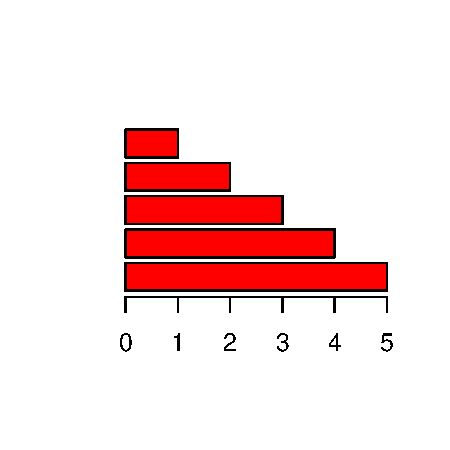
\includegraphics[width=\textheight]{graphiques/beamer-Barplot2-1} 

}



\end{knitrout}


	\subsection{Changement dans l'environnement p�re...}

En fait il existe une possibilit� pour changer la valeur d'une variable dans l'environnement p�re.

C'est pratique pour modifier une \df encombrante par exemple.



\begin{knitrout}\footnotesize
\definecolor{shadecolor}{rgb}{0.969, 0.969, 0.969}\color{fgcolor}\begin{kframe}
\begin{alltt}
\hlstd{i} \hlkwb{<-} \hlnum{1}
\hlstd{a} \hlkwb{<-} \hlkwa{function} \hlstd{(}\hlkwc{x}\hlstd{) \{ i} \hlkwb{<-} \hlnum{2} \hlstd{\}}
\hlstd{i}
\end{alltt}
\begin{verbatim}
## [1] 1
\end{verbatim}
\begin{alltt}
\hlstd{i} \hlkwb{<-} \hlnum{1}
\hlstd{a} \hlkwb{<-} \hlkwa{function} \hlstd{(}\hlkwc{x}\hlstd{) \{ i} \hlkwb{<<-} \hlnum{2} \hlstd{\}}
\hlkwd{a}\hlstd{(}\hlnum{7}\hlstd{);i;}
\end{alltt}
\begin{verbatim}
## [1] 2
\end{verbatim}
\end{kframe}
\end{knitrout}



L'inconv�nient est que cela rend la fonction d�pendante de l'environnement p�re et du nom des variables dans celui-ci.

Son utilisation est donc � limiter sauf cas particuliers.



\section{Les structures de contr�le}

	\subsection{Les boucles}

  Les boucles sont � �viter car lentes � ex�cuter. Il faut leur pr�f�rer les fonctions de type \emph{apply}. La syntaxe d'une boucle est la suivante...

\begin{verbatim}
for ( mavar in sequence ) {
       ... code R...
}
\end{verbatim}

  la variable \emph{mavar} prend � chaque it�ration un �lement de \emph{sequence} dans l'ordre. Les it�rations peuvent se faire sur un type quelconque comme des entiers (usuels) mais �galement un vecteur de \character par exemple. Ou bien un vecteur de fonctions\dots 


	\subsection{Les tests}

        Les tests ont la structure suivante~:

\begin{knitrout}\footnotesize
\definecolor{shadecolor}{rgb}{0.969, 0.969, 0.969}\color{fgcolor}\begin{kframe}
\begin{alltt}
\hlkwd{if} ( valeur ) \{
       ... code R...
\}
\end{alltt}
\end{kframe}
\end{knitrout}
        ou
\begin{knitrout}\footnotesize
\definecolor{shadecolor}{rgb}{0.969, 0.969, 0.969}\color{fgcolor}\begin{kframe}
\begin{alltt}
\hlkwd{if} ( valeur ) \{
 ... code R...
\} else \{
... code R...
\}
\end{alltt}
\end{kframe}
\end{knitrout}



  La condition est execut� si la valeur est \emph{TRUE}, \emph{T} ou diff�rent de 0.

  Attention, le vecteur bool�en doit �tre de longueur 1. A
  l'int�rieur d'un test, R attend \emph{T} ou \emph{F} et pas \emph{c(T,F,T)}.



        Les fonctions � conna�tre sont donc \emph{any} qui renvoie vrai si
        au moins un �lement est vrai dans le vecteur pass� en argument.

        Et la fonction \emph{all} qui renvoie vrai si toutes les valeurs du
        vecteur pass� en argument sont vrai.




        Des op�rations sur les bool�ens disponibles~:

\begin{itemize}

\item qui \textit{renvoient} des vecteurs de longueur plus grande que 1

\begin{verbatim}
& : et
| : ou
\end{verbatim}

\item qui \textit{renvoient} des vecteurs de longueur 1

\begin{verbatim}
&& : et
|| : ou
\end{verbatim}

\end{itemize}



        Il y a une fonction � conna�tre car tr�s rapide et tr�s simple~:
\begin{verbatim}
ifelse( mavar, valeur_si_vrai, valeur_si_faux )
\end{verbatim}

        Par exemple~:
\begin{knitrout}\footnotesize
\definecolor{shadecolor}{rgb}{0.969, 0.969, 0.969}\color{fgcolor}\begin{kframe}
\begin{alltt}
\hlkwd{ifelse}\hlstd{(} \hlkwd{rnorm}\hlstd{(}\hlnum{10}\hlstd{)} \hlopt{>} \hlnum{0}\hlstd{,} \hlnum{1}\hlstd{,} \hlopt{-}\hlnum{1} \hlstd{)}
\end{alltt}
\begin{verbatim}
##  [1]  1 -1  1  1 -1  1  1 -1  1  1
\end{verbatim}
\end{kframe}
\end{knitrout}


	\subsection{Stopper l'ex�cution}

  La fonction \emph{stop} permet d'arr�ter un script et
  d'indiquer une erreur.

\begin{verbatim}
if ( class != "numeric" ) stop("Non numerique")
\end{verbatim}


\section{Les fonctions apply}

	\subsection{Les diff�rentes fonctions}

        Dans la famille \emph{apply}, on a en fait~:

\begin{verbatim}
lapply(X, FUN, ...)
sapply(X, FUN, ..., simplify = TRUE, USE.NAMES = TRUE)
vapply(X, FUN, FUN.VALUE, ..., USE.NAMES = TRUE)
replicate(n, expr, simplify = TRUE)
\end{verbatim}



    Par exemple, nous voulons par exemple r�cup�rer les
    quantiles de toutes les variables num�riques. Pour cela, nous
    utilisons la fonction \emph{apply}.



\begin{knitrout}\footnotesize
\definecolor{shadecolor}{rgb}{0.969, 0.969, 0.969}\color{fgcolor}\begin{kframe}
\begin{alltt}
\hlstd{(r} \hlkwb{<-} \hlkwd{apply}\hlstd{(iris[,}\hlnum{1}\hlopt{:}\hlnum{4}\hlstd{],}\hlnum{2}\hlstd{,quantile))}
\end{alltt}
\begin{verbatim}
##      Sepal.Length Sepal.Width Petal.Length
## 0%            4.3         2.0         1.00
## 25%           5.1         2.8         1.60
## 50%           5.8         3.0         4.35
## 75%           6.4         3.3         5.10
## 100%          7.9         4.4         6.90
##      Petal.Width
## 0%           0.1
## 25%          0.3
## 50%          1.3
## 75%          1.8
## 100%         2.5
\end{verbatim}
\end{kframe}
\end{knitrout}



        La fonction \emph{apply} permet d'appliquer une fonction sur une \df dans le sens~:
        \begin{itemize}
          \item des lignes, ligne par ligne, avec l'indice 1
         \item des colonnes, colonne par colonne, avec l'indice 2
         \item cellule par cellule avec l'indice \emph{1:2} (ou \emph{c(1,2)})
       \end{itemize}


	\subsection{Les fonctions apply}

        Donc pour l'exemple pr�c�dent, calculer les quantiles, on demande �
        R de passer chaque colonne � la fonction quantile.

        La fonction quantile rend un vecteur et R se ``d�brouille'' tout
        seul avec les vecteurs r�sultats~: il les aggr�ge sous forme
        de matrice.


	\subsection{Les diff�rentes fonctions}

  Par exemple sapply, prends comme argument une \liste et renvoie
  quelque chose de simplifi� quand elle le peut.

        Par exemple pour retrouver les colonnes numeric d'une \df...
\begin{knitrout}\footnotesize
\definecolor{shadecolor}{rgb}{0.969, 0.969, 0.969}\color{fgcolor}\begin{kframe}
\begin{alltt}
\hlkwd{sapply}\hlstd{( iris, is.numeric )}
\end{alltt}
\begin{verbatim}
## Sepal.Length  Sepal.Width Petal.Length 
##         TRUE         TRUE         TRUE 
##  Petal.Width      Species 
##         TRUE        FALSE
\end{verbatim}
\end{kframe}
\end{knitrout}


  Pourquoi �a marche ?

  Parce que \df peut �tre convertie en \liste puis la fonction est appliqu�e � chaque �lement de la \liste.

\begin{knitrout}\footnotesize
\definecolor{shadecolor}{rgb}{0.969, 0.969, 0.969}\color{fgcolor}\begin{kframe}
\begin{alltt}
\hlkwd{str}\hlstd{(}\hlkwd{as.list}\hlstd{(iris))}
\end{alltt}
\begin{verbatim}
## List of 5
##  $ Sepal.Length: num [1:150] 5.1 4.9 4.7 4.6 5 5.4 4.6 5 4.4 4.9 ...
##  $ Sepal.Width : num [1:150] 3.5 3 3.2 3.1 3.6 3.9 3.4 3.4 2.9 3.1 ...
##  $ Petal.Length: num [1:150] 1.4 1.4 1.3 1.5 1.4 1.7 1.4 1.5 1.4 1.5 ...
##  $ Petal.Width : num [1:150] 0.2 0.2 0.2 0.2 0.2 0.4 0.3 0.2 0.2 0.1 ...
##  $ Species     : Factor w/ 3 levels "setosa","versicolor",..: 1 1 1 1 1 1 1 1 1 1 ...
\end{verbatim}
\end{kframe}
\end{knitrout}



  L'avantage de \emph{sapply} est qu'elle renvoie un objet
  simplifi� par rapport � \emph{lapply}.

  \emph{vapply} est identique avec un contr�le sur le type d'objet renvoy�.



    \emph{replicate} est une fonction extr�mement utile. Un des
    gros avantages de R est qu'il permet tr�s aisement de simuler
    des donn�es.

    \emph{replicate} est une des fonctions qui permet de le faire en r�p�tant une boucle tout en g�n�rant des nombres al�atoires.


  \subsection{les autres fonctions apply}

  \textit{mapply} se distingue car elle peut prendre plusieurs arguments.
  
  \textit{vapply} est utilis� sur les vecteurs et permet la v�rification du type en sortie.
  
  \dots


	\subsection{Les diff�rentes fonctions}

\begin{knitrout}\footnotesize
\definecolor{shadecolor}{rgb}{0.969, 0.969, 0.969}\color{fgcolor}\begin{kframe}
\begin{alltt}
\hlkwd{set.seed}\hlstd{(}\hlnum{42}\hlstd{)}
\hlkwd{system.time}\hlstd{(}
\hlstd{res1} \hlkwb{<-} \hlkwd{replicate}\hlstd{(} \hlnum{10000}\hlstd{,} \hlkwa{function}\hlstd{() \{} \hlkwd{return}\hlstd{(}\hlkwd{mean}\hlstd{(}\hlkwd{rnorm}\hlstd{(}\hlnum{1000}\hlstd{))) \} )}
\hlstd{)}
\end{alltt}
\begin{verbatim}
##    user  system elapsed 
##   0.008   0.000   0.006
\end{verbatim}
\begin{alltt}
\hlkwd{system.time}\hlstd{(\{}
\hlstd{res2} \hlkwb{<-} \hlkwd{numeric}\hlstd{(}\hlnum{10000}\hlstd{)}
\hlkwa{for} \hlstd{( ii} \hlkwa{in} \hlnum{1}\hlopt{:}\hlnum{10000} \hlstd{) \{ res2[ii]} \hlkwb{<-} \hlkwd{mean}\hlstd{(}\hlkwd{rnorm}\hlstd{(}\hlnum{1000}\hlstd{)) \}}
\hlstd{\})}
\end{alltt}
\begin{verbatim}
##    user  system elapsed 
##   0.868   0.000   0.870
\end{verbatim}
\end{kframe}
\end{knitrout}



  Ce qu'il ne faut surtout pas faire~:

\begin{knitrout}\footnotesize
\definecolor{shadecolor}{rgb}{0.969, 0.969, 0.969}\color{fgcolor}\begin{kframe}
\begin{alltt}
\hlkwd{system.time}\hlstd{(\{}
\hlstd{res2} \hlkwb{<-} \hlkwd{c}\hlstd{()}
\hlkwa{for} \hlstd{( ii} \hlkwa{in} \hlnum{1}\hlopt{:}\hlnum{10000} \hlstd{) \{ res2} \hlkwb{<-} \hlkwd{c}\hlstd{( res2,} \hlkwd{mean}\hlstd{(}\hlkwd{rnorm}\hlstd{(}\hlnum{1000}\hlstd{)) ) \}}
\hlstd{\})}
\end{alltt}
\begin{verbatim}
##    user  system elapsed 
##   1.028   0.000   1.030
\end{verbatim}
\end{kframe}
\end{knitrout}


	\subsection{Un exemple, le bootstrap...}



\begin{knitrout}\footnotesize
\definecolor{shadecolor}{rgb}{0.969, 0.969, 0.969}\color{fgcolor}\begin{kframe}
\begin{alltt}
\hlstd{n} \hlkwb{<-} \hlnum{1000}
\hlkwd{set.seed}\hlstd{(}\hlnum{42}\hlstd{)}
\hlstd{b} \hlkwb{<-} \hlkwd{replicate}\hlstd{( n,} \hlkwd{mean}\hlstd{(} \hlkwd{sample}\hlstd{( patient}\hlopt{$}\hlstd{totalechelle,}
                                 \hlkwd{length}\hlstd{(patient}\hlopt{$}\hlstd{totalechelle),}
                                 \hlkwc{replace} \hlstd{= T ),} \hlkwc{na.rm}\hlstd{=T ) )}
\hlkwd{mean}\hlstd{((b}\hlopt{-}\hlkwd{mean}\hlstd{(b))}\hlopt{^}\hlnum{2}\hlstd{)}
\end{alltt}
\end{kframe}
\end{knitrout}


	\subsection{Les boucles}

\begin{knitrout}\footnotesize
\definecolor{shadecolor}{rgb}{0.969, 0.969, 0.969}\color{fgcolor}\begin{kframe}
\begin{alltt}
\hlkwa{for} \hlstd{( ii} \hlkwa{in} \hlnum{1}\hlopt{:}\hlnum{4} \hlstd{) \{} \hlkwd{print}\hlstd{(ii) \}}
\end{alltt}
\begin{verbatim}
## [1] 1
## [1] 2
## [1] 3
## [1] 4
\end{verbatim}
\end{kframe}
\end{knitrout}

\begin{knitrout}\footnotesize
\definecolor{shadecolor}{rgb}{0.969, 0.969, 0.969}\color{fgcolor}\begin{kframe}
\begin{alltt}
\hlkwa{for} \hlstd{( ww} \hlkwa{in} \hlstd{LETTERS[}\hlnum{1}\hlopt{:}\hlnum{4}\hlstd{] ) \{} \hlkwd{print}\hlstd{(ww) \}}
\end{alltt}
\begin{verbatim}
## [1] "A"
## [1] "B"
## [1] "C"
## [1] "D"
\end{verbatim}
\end{kframe}
\end{knitrout}



En vrai, une boucle pourrait servir � �a~:
\begin{knitrout}\footnotesize
\definecolor{shadecolor}{rgb}{0.969, 0.969, 0.969}\color{fgcolor}\begin{kframe}
\begin{alltt}
\hlstd{a} \hlkwb{<-} \hlkwd{numeric}\hlstd{(}\hlnum{4}\hlstd{)}
\hlkwa{for} \hlstd{( ii} \hlkwa{in} \hlnum{1}\hlopt{:}\hlnum{4} \hlstd{) \{ a[ii]} \hlkwb{<-} \hlkwd{mean}\hlstd{(}\hlkwd{rnorm}\hlstd{(}\hlnum{1000}\hlstd{)) \}}
\hlstd{a}
\end{alltt}
\begin{verbatim}
## [1] -0.057470355  0.005562816  0.008292973
## [4] -0.009122556
\end{verbatim}
\end{kframe}
\end{knitrout}

Ce qui s'�crit plus simplement et surtout beaucoup plus efficacement~:
\begin{knitrout}\footnotesize
\definecolor{shadecolor}{rgb}{0.969, 0.969, 0.969}\color{fgcolor}\begin{kframe}
\begin{alltt}
\hlstd{a} \hlkwb{<-} \hlkwd{vapply}\hlstd{(}\hlnum{1}\hlopt{:}\hlnum{4}\hlstd{,}\hlkwa{function}\hlstd{(}\hlkwc{x}\hlstd{)} \hlkwd{mean}\hlstd{(}\hlkwd{rnorm}\hlstd{(x)),}\hlkwd{numeric}\hlstd{(}\hlnum{1}\hlstd{))}
\hlstd{a}
\end{alltt}
\begin{verbatim}
## [1]  0.7700131  1.2346050 -0.5141222  0.2071179
\end{verbatim}
\end{kframe}
\end{knitrout}



En vrai, une boucle pourrait servir � �a~:
\begin{knitrout}\footnotesize
\definecolor{shadecolor}{rgb}{0.969, 0.969, 0.969}\color{fgcolor}\begin{kframe}
\begin{alltt}
\hlstd{vars} \hlkwb{<-} \hlkwd{colnames}\hlstd{(iris)[}\hlkwd{sapply}\hlstd{(iris,is.numeric)]}
\hlkwa{for} \hlstd{( ii} \hlkwa{in} \hlstd{vars ) \{ iris[ii]} \hlkwb{<-} \hlkwd{scale}\hlstd{(iris[ii]) \}}
\end{alltt}
\end{kframe}
\end{knitrout}

Ce qui s'�crit plus simplement et surtout beaucoup plus efficacement~:
\begin{knitrout}\footnotesize
\definecolor{shadecolor}{rgb}{0.969, 0.969, 0.969}\color{fgcolor}\begin{kframe}
\begin{alltt}
\hlstd{vars} \hlkwb{<-} \hlkwd{colnames}\hlstd{(iris)[}\hlkwd{sapply}\hlstd{(iris,is.numeric)]}
\hlstd{iris[,vars]} \hlkwb{<-} \hlkwd{apply}\hlstd{(iris[,vars],}\hlnum{2}\hlstd{,scale)}
\end{alltt}
\end{kframe}
\end{knitrout}




Une utilisation justifi�e des boucles.

\begin{knitrout}\footnotesize
\definecolor{shadecolor}{rgb}{0.969, 0.969, 0.969}\color{fgcolor}\begin{kframe}
\begin{alltt}
\hlkwa{for} \hlstd{( ww} \hlkwa{in} \hlkwd{c}\hlstd{(} \hlkwa{function}\hlstd{(}\hlkwc{x}\hlstd{) \{x}\hlopt{^}\hlnum{1}\hlstd{\},} \hlkwa{function}\hlstd{(}\hlkwc{x}\hlstd{) \{x}\hlopt{^}\hlnum{2}\hlstd{\},} \hlkwa{function}\hlstd{(}\hlkwc{x}\hlstd{) \{x}\hlopt{^}\hlnum{3}\hlstd{\} ) ) \{} \hlkwd{print}\hlstd{(}\hlkwd{ww}\hlstd{(}\hlnum{2}\hlstd{)) \}}
\end{alltt}
\begin{verbatim}
## [1] 2
## [1] 4
## [1] 8
\end{verbatim}
\end{kframe}
\end{knitrout}

En fait, non
\begin{knitrout}\footnotesize
\definecolor{shadecolor}{rgb}{0.969, 0.969, 0.969}\color{fgcolor}\begin{kframe}
\begin{alltt}
\hlstd{power} \hlkwb{<-} \hlkwa{function}\hlstd{(}\hlkwc{n}\hlstd{,}\hlkwc{x}\hlstd{) \{x}\hlopt{^}\hlstd{n\}}
\hlkwd{sapply}\hlstd{(}\hlkwd{as.list}\hlstd{(}\hlnum{1}\hlopt{:}\hlnum{3}\hlstd{),power,}\hlkwc{x}\hlstd{=}\hlnum{2}\hlstd{)}
\end{alltt}
\begin{verbatim}
## [1] 2 4 8
\end{verbatim}
\end{kframe}
\end{knitrout}


	\subsection{Split...}

  La fonction \emph{split} permet de d�couper une \df en
  fonction des modalit�s d'une variable et de r�cup�rer une
  \liste en sortie avec pour chaque modalit� la partie correspondante de la \df.

\begin{knitrout}\footnotesize
\definecolor{shadecolor}{rgb}{0.969, 0.969, 0.969}\color{fgcolor}\begin{kframe}
\begin{alltt}
\hlkwd{str}\hlstd{(}\hlkwd{split}\hlstd{(iris,}\hlkwd{factor}\hlstd{(iris}\hlopt{$}\hlstd{Species)))}
\end{alltt}
\begin{verbatim}
## List of 3
##  $ setosa    :'data.frame':	50 obs. of  5 variables:
##   ..$ Sepal.Length: num [1:50] -0.898 -1.139 -1.381 -1.501 -1.018 ...
##   ..$ Sepal.Width : num [1:50] 1.0156 -0.1315 0.3273 0.0979 1.245 ...
##   ..$ Petal.Length: num [1:50] -1.34 -1.34 -1.39 -1.28 -1.34 ...
##   ..$ Petal.Width : num [1:50] -1.31 -1.31 -1.31 -1.31 -1.31 ...
##   ..$ Species     : Factor w/ 3 levels "setosa","versicolor",..: 1 1 1 1 1 1 1 1 1 1 ...
##  $ versicolor:'data.frame':	50 obs. of  5 variables:
##   ..$ Sepal.Length: num [1:50] 1.397 0.672 1.276 -0.415 0.793 ...
##   ..$ Sepal.Width : num [1:50] 0.3273 0.3273 0.0979 -1.7375 -0.5904 ...
##   ..$ Petal.Length: num [1:50] 0.534 0.42 0.647 0.137 0.477 ...
##   ..$ Petal.Width : num [1:50] 0.263 0.394 0.394 0.132 0.394 ...
##   ..$ Species     : Factor w/ 3 levels "setosa","versicolor",..: 2 2 2 2 2 2 2 2 2 2 ...
##  $ virginica :'data.frame':	50 obs. of  5 variables:
##   ..$ Sepal.Length: num [1:50] 0.5515 -0.0523 1.5176 0.5515 0.793 ...
##   ..$ Sepal.Width : num [1:50] 0.557 -0.82 -0.132 -0.361 -0.132 ...
##   ..$ Petal.Length: num [1:50] 1.27 0.76 1.21 1.04 1.16 ...
##   ..$ Petal.Width : num [1:50] 1.706 0.919 1.182 0.788 1.313 ...
##   ..$ Species     : Factor w/ 3 levels "setosa","versicolor",..: 3 3 3 3 3 3 3 3 3 3 ...
\end{verbatim}
\end{kframe}
\end{knitrout}



  \subsection{do.call}

  \textit{do.call} est une fonction assez complexe. Elle permet notamment de d�finir l'environnement dans lequel ex�cut� une commande R. 
  
  Toutefois elle a une utilisation simple � conna�tre. Elle permet en une ligne d'aggr�ger des r�sultats provenant d'une commande lapply. 
  
\begin{knitrout}\footnotesize
\definecolor{shadecolor}{rgb}{0.969, 0.969, 0.969}\color{fgcolor}\begin{kframe}
\begin{alltt}
\hlstd{stats} \hlkwb{<-} \hlkwa{function} \hlstd{(}\hlkwc{x}\hlstd{) \{} \hlkwd{c}\hlstd{(}
  \hlkwd{quantile}\hlstd{( x}\hlopt{$}\hlstd{Sepal.Length,}\hlkwc{probs}\hlstd{=}\hlkwd{c}\hlstd{(}\hlnum{0}\hlstd{,}\hlnum{0.25}\hlstd{,}\hlnum{0.5}\hlstd{,}\hlnum{0.75}\hlstd{,}\hlnum{1}\hlstd{)),}
  \hlkwd{mean}\hlstd{(x}\hlopt{$}\hlstd{Sepal.Length),}
  \hlkwd{sd}\hlstd{(x}\hlopt{$}\hlstd{Sepal.Length) )}
\hlstd{\}}
\hlstd{res} \hlkwb{<-} \hlkwd{lapply}\hlstd{(} \hlkwd{split}\hlstd{(iris,iris}\hlopt{$}\hlstd{Species), stats )}
\hlkwd{str}\hlstd{(res)}
\end{alltt}
\begin{verbatim}
## List of 3
##  $ setosa    : Named num [1:7] -1.8638 -1.26 -1.0184 -0.7769 -0.0523 ...
##   ..- attr(*, "names")= chr [1:7] "0%" "25%" "50%" "75%" ...
##  $ versicolor: Named num [1:7] -1.1392 -0.2939 0.0684 0.5515 1.3968 ...
##   ..- attr(*, "names")= chr [1:7] "0%" "25%" "50%" "75%" ...
##  $ virginica : Named num [1:7] -1.139 0.461 0.793 1.276 2.484 ...
##   ..- attr(*, "names")= chr [1:7] "0%" "25%" "50%" "75%" ...
\end{verbatim}
\end{kframe}
\end{knitrout}



\begin{knitrout}\footnotesize
\definecolor{shadecolor}{rgb}{0.969, 0.969, 0.969}\color{fgcolor}\begin{kframe}
\begin{alltt}
\hlkwd{do.call}\hlstd{( rbind, res )}
\end{alltt}
\begin{verbatim}
##                  0%        25%         50%
## setosa     -1.86378 -1.2599638 -1.01843718
## versicolor -1.13920 -0.2938574  0.06843254
## virginica  -1.13920  0.4609133  0.79301235
##                   75%        100%           
## setosa     -0.7769106 -0.05233076 -1.0111914
## versicolor  0.5514857  1.39682886  0.1119073
## virginica   1.2760656  2.48369858  0.8992841
##                     
## setosa     0.4256782
## versicolor 0.6233453
## virginica  0.7679092
\end{verbatim}
\end{kframe}
\end{knitrout}


  Si l'exemple peut �tre r�alis� par exemple avec plyr, il est bonne illustration de \textit{do.call}.
  
  Plut�t qu'une matrice, si les r�sultats sont de types diff�rents, on peut �crire dans certains cas~:
  
\begin{knitrout}\footnotesize
\definecolor{shadecolor}{rgb}{0.969, 0.969, 0.969}\color{fgcolor}\begin{kframe}
\begin{alltt}
\hlkwd{do.call}\hlstd{( data.frame, res )}
\end{alltt}
\end{kframe}
\end{knitrout}


  \subsection{lapply}

  La fonction \textit{lapply} est une fonction dont l'utilisation doit cro�tre avec l'exp�rience. Elle est centrale dans R et s'annonce de plus en plus indispensable car elle est � la base des fonctions de vectorisation des calculs dans R.
  
  Par exemple, un jackknife, est tr�s facile � r�aliser avec une fonction \textit{lapply}.

\begin{knitrout}\footnotesize
\definecolor{shadecolor}{rgb}{0.969, 0.969, 0.969}\color{fgcolor}\begin{kframe}
\begin{alltt}
\hlstd{mm} \hlkwb{<-} \hlkwd{mean}\hlstd{(iris[,}\hlstr{"Sepal.Length"}\hlstd{])}
\hlstd{res} \hlkwb{<-} \hlkwd{sapply}\hlstd{(} \hlkwd{as.list}\hlstd{(}\hlnum{1}\hlopt{:}\hlkwd{nrow}\hlstd{(iris)),}
               \hlkwa{function} \hlstd{(}\hlkwc{x}\hlstd{) \{}
                 \hlstd{(}\hlkwd{mean}\hlstd{(iris[}\hlopt{-}\hlstd{x,}\hlstr{"Sepal.Length"}\hlstd{])}\hlopt{-}\hlstd{mm)}\hlopt{^}\hlnum{2}
\hlstd{\} )}
\hlstd{vv} \hlkwb{<-} \hlkwd{sqrt}\hlstd{(}\hlkwd{sum}\hlstd{(}\hlkwd{as.numeric}\hlstd{(res))}\hlopt{/}\hlstd{(}\hlkwd{nrow}\hlstd{(iris)}\hlopt{*}\hlstd{(}\hlkwd{nrow}\hlstd{(iris)}\hlopt{-}\hlnum{1}\hlstd{)))}
\hlkwd{paste}\hlstd{(} \hlstr{"["}\hlstd{,} \hlkwd{qt}\hlstd{(}\hlnum{0.025}\hlstd{,}\hlkwd{nrow}\hlstd{(iris)}\hlopt{-}\hlnum{1}\hlstd{)}\hlopt{*}\hlstd{vv}\hlopt{+}\hlstd{mm,}
       \hlstr{":"}\hlstd{,} \hlkwd{qt}\hlstd{(}\hlnum{0.975}\hlstd{,}\hlkwd{nrow}\hlstd{(iris)}\hlopt{-}\hlnum{1}\hlstd{)}\hlopt{*}\hlstd{vv}\hlopt{+}\hlstd{mm,} \hlstr{"]"} \hlstd{)}
\end{alltt}
\begin{verbatim}
## [1] "[ -0.00108282416339017 : 0.00108282416339017 ]"
\end{verbatim}
\end{kframe}
\end{knitrout}


  \subsection{Calculs parall�les}

  La vectorisation est pour l'instant assez peu document�. Il existe l'ouvrage de McCallum (2012) et quelques ressources dans les blogs sur R.
  
  Sous les syst�mes de type GNU/Linux, la vectorisation sur une m�me machine est d'une simplicit� �vang�lique. Il suffit de charger le paquet \textit{parallel} et de sp�cifier le nombre de processeurs � utiliser et d'utiliser la fonction \textit{mclapply}.
  
  Ce qui donne pratiquement le m�me code que pr�cedemment pour un jackknife\dots
  


\begin{knitrout}\footnotesize
\definecolor{shadecolor}{rgb}{0.969, 0.969, 0.969}\color{fgcolor}\begin{kframe}
\begin{alltt}
\hlstd{mm} \hlkwb{<-} \hlkwd{mean}\hlstd{(iris[,}\hlstr{"Sepal.Length"}\hlstd{])}
\hlstd{res} \hlkwb{<-} \hlkwd{mclapply}\hlstd{(} \hlkwd{as.list}\hlstd{(}\hlnum{1}\hlopt{:}\hlkwd{nrow}\hlstd{(iris)),} \hlkwa{function} \hlstd{(}\hlkwc{x}\hlstd{)}
  \hlstd{(}\hlkwd{mean}\hlstd{(iris[}\hlopt{-}\hlstd{x,}\hlstr{"Sepal.Length"}\hlstd{])}\hlopt{-}\hlstd{mm)}\hlopt{^}\hlnum{2}\hlstd{,}
  \hlkwc{mc.cores}\hlstd{=}\hlnum{4}
\hlstd{)}

\hlstd{vv} \hlkwb{<-} \hlkwd{sqrt}\hlstd{(}\hlkwd{sum}\hlstd{(}\hlkwd{as.numeric}\hlstd{(res))}\hlopt{/}\hlstd{(}\hlkwd{nrow}\hlstd{(iris)}\hlopt{*}\hlstd{(}\hlkwd{nrow}\hlstd{(iris)}\hlopt{-}\hlnum{1}\hlstd{)))}

\hlkwd{paste}\hlstd{(} \hlstr{"["}\hlstd{,} \hlkwd{qt}\hlstd{(}\hlnum{0.025}\hlstd{,}\hlkwd{nrow}\hlstd{(iris))}\hlopt{*}\hlstd{vv}\hlopt{+}\hlstd{mm,} \hlstr{":"}\hlstd{,}
       \hlkwd{qt}\hlstd{(}\hlnum{0.975}\hlstd{,}\hlkwd{nrow}\hlstd{(iris))}\hlopt{*}\hlstd{vv}\hlopt{+}\hlstd{mm,} \hlstr{"]"} \hlstd{)}
\end{alltt}
\end{kframe}
\end{knitrout}



  Avec ce m�canisme, 10 processus R vont �tre lanc�s en parall�le sur la machine. La m�moire n�cessaire  � chaque processus doit �tre disponible. Ce qui revient � demander � la machine 4 fois la m�moire n�cessaire � l'�xecution du processus.
  
  Le syst�me utilise la commande \textit{fork} du syst�me d'exploitation. Par cons�quent, chaque processus r�cup�re l'environnement (variables) et paquets de la session courante. Pratique.
  
  Dans le cas de simulation, il est n�cessaire de bien lire l'aide du package pour obtenir selon ses besoins des seeds parall�les ou asynchrone.
  
  

  Dans le cas de machine Windows, cette m�thode ne fonctionne pas en raison du fonctionnement de Windows (quelque soit sa version).
  
  Aussi dans ce cas et pour faire du calcul parall�le en g�rant plus finement les ressources mat�riels et plusieurs ordinateurs quelque soit leur syst�me d'exploitation, il est n�cessaire de passer plut�t par l'utilisation des framework SNOW et MPI par exemple.
  
  L'utilisation est plus d�licate car l'utilisateur doit notamment indiquer quelles variables, quels paquets, \dots doivent �tre inject�s dans les processus avant le lancement du calcul.
  
  


  Une vue enti�re est d�di�e au probl�me des calculs lourds\dots
  
  \vspace{0.1cm}
  
  \href{http://cran.r-project.org/web/views/HighPerformanceComputing.html}{High-Performance and Parallel Computing with R}
  



\section{L'automatisation des scripts}

	\subsection{Lancement d'un script automatiquement}

  Pour lancer un script automatiquement, on peut le faire dans
  un fichier \emph{batch}, c'est-�-dire un petit executable qui se
  termine en \emph{.bat} sous \Windows.

  Il est conseill� de mettre le chemin de R dans le PATH \Windows
  pour ne pas avoir � taper le chemin complet d'acc�s � R.

  On peut ainsi appeler un script~:

\begin{verbatim}
R -f Monscript.R
\end{verbatim}



  Mais R a une commande sp�cialement con�ues pour r�aliser des
  op�rations depuis des fichiers ex�cutables...

\begin{verbatim}
R CMD BATCH Monscript.R
\end{verbatim}

  Un fichier \emph{.Rout} est g�n�r� automatiquement et contient
  tout ce qui est apparu dans la console.


	\subsection{\emph{source}}

  La fonction \emph{source} permet d'ex�cuter le contenu d'un
  script depuis un autre script.

  Cela permet par exemple de stocker des fonctions g�n�riques
  puis de les rappeler en suite sans faire de paquets...

\begin{verbatim}
source("MesFonctions.R")
monbarplot(iris$Species)
\end{verbatim}


	\subsection{Les r�gles de r�daction des scripts}

  R est un langage de programmation...

  {\textbf Pour la relecture et la lisibilit� du code penser � commenter
  et � indenter !}



    Il est souvent plus simple d'utiliser un �diteur de texte tel
    que \emph{emacs} ou \emph{notepad++} pour profiter de la coloration
    syntaxique puis de copier-coller dans la console R.

    ou \emph{RStudio}.






\documentclass{beamer}\usepackage[]{graphicx}\usepackage[]{color}
%% maxwidth is the original width if it is less than linewidth
%% otherwise use linewidth (to make sure the graphics do not exceed the margin)
\makeatletter
\def\maxwidth{ %
  \ifdim\Gin@nat@width>\linewidth
    \linewidth
  \else
    \Gin@nat@width
  \fi
}
\makeatother

\definecolor{fgcolor}{rgb}{0.345, 0.345, 0.345}
\newcommand{\hlnum}[1]{\textcolor[rgb]{0.686,0.059,0.569}{#1}}%
\newcommand{\hlstr}[1]{\textcolor[rgb]{0.192,0.494,0.8}{#1}}%
\newcommand{\hlcom}[1]{\textcolor[rgb]{0.678,0.584,0.686}{\textit{#1}}}%
\newcommand{\hlopt}[1]{\textcolor[rgb]{0,0,0}{#1}}%
\newcommand{\hlstd}[1]{\textcolor[rgb]{0.345,0.345,0.345}{#1}}%
\newcommand{\hlkwa}[1]{\textcolor[rgb]{0.161,0.373,0.58}{\textbf{#1}}}%
\newcommand{\hlkwb}[1]{\textcolor[rgb]{0.69,0.353,0.396}{#1}}%
\newcommand{\hlkwc}[1]{\textcolor[rgb]{0.333,0.667,0.333}{#1}}%
\newcommand{\hlkwd}[1]{\textcolor[rgb]{0.737,0.353,0.396}{\textbf{#1}}}%

\usepackage{framed}
\makeatletter
\newenvironment{kframe}{%
 \def\at@end@of@kframe{}%
 \ifinner\ifhmode%
  \def\at@end@of@kframe{\end{minipage}}%
  \begin{minipage}{\columnwidth}%
 \fi\fi%
 \def\FrameCommand##1{\hskip\@totalleftmargin \hskip-\fboxsep
 \colorbox{shadecolor}{##1}\hskip-\fboxsep
     % There is no \\@totalrightmargin, so:
     \hskip-\linewidth \hskip-\@totalleftmargin \hskip\columnwidth}%
 \MakeFramed {\advance\hsize-\width
   \@totalleftmargin\z@ \linewidth\hsize
   \@setminipage}}%
 {\par\unskip\endMakeFramed%
 \at@end@of@kframe}
\makeatother

\definecolor{shadecolor}{rgb}{.97, .97, .97}
\definecolor{messagecolor}{rgb}{0, 0, 0}
\definecolor{warningcolor}{rgb}{1, 0, 1}
\definecolor{errorcolor}{rgb}{1, 0, 0}
\newenvironment{knitrout}{}{} % an empty environment to be redefined in TeX

\usepackage{alltt}
\usetheme[compress]{Singapore}
\useoutertheme{miniframes}

% \documentclass{beamer}
%\usetheme{Warsaw}

% Pour les documents en francais...
	\usepackage[latin1]{inputenc}
	\usepackage[french]{babel}
	\usepackage[french]{varioref}

% Math�matiques
	\usepackage{amsmath}

% Caracteres speciaux suppl�mentaires
	\usepackage{latexsym,amsfonts}

% A documenter
	\usepackage{moreverb}

% Macros pour les paquets
	\usepackage{array}  			% N�cessaires pour les tableaux de la macro Excel.

% Outil suppl�mentaire pour les tableaux
	\usepackage{multirow}
	\usepackage{booktabs}
	\usepackage{xcolor} % alternating row colors in table, incompatible avec certains modules
	\usepackage{longtable}
	\usepackage{colortbl}

% Pour ins�rer des graphiques
	\usepackage{graphicx} 			% Graphique simples
	\usepackage{subfigure}			% Graphiques multiples

% Pour ins�rer des couleurs
	\usepackage{color}

% Rotation des objets et des pages
%	\usepackage{rotating}
%	\usepackage{lscape}

% Pour insrer du code source, LaTeX ou SAS par exemple.
	\usepackage{verbatim}
        \usepackage{moreverb}
	\usepackage{listings}
	\usepackage{fancyvrb}

%	\lstset{language=SAS,numbers=left}		% Par dfaut le listing est en SAS

% Pour ins�rer des hyperliens
  \usepackage{hyperref}

% American Psychological Association (for bibliographic references).
	\usepackage{apacite}

% Pour l'utilisation des macros
	\usepackage{xspace}

% Pour l'utilisation de notes en fin de document.
%	\usepackage{endnotes}

% Array
%	\usepackage{multirow}
%	\usepackage{booktabs}

% Rotation
%	\usepackage{rotating}

% En t�tes et pieds de pages
%	\usepackage{fancyhdr}
%	\usepackage{lastpage}


% Page layout

% By LaTeX commands
%\setlength{\oddsidemargin}{0cm}
%\setlength{\textwidth}{16cm}
%\setlength{\textheight}{24cm}
%\setlength{\topmargin}{-1cm}
%\setlength{\marginparsep}{0.2cm}

% fancyheader parameters
%\pagestyle{fancy}

%\fancyfoot[L]{{\small Formation \LaTeX, DEPP}}
%\fancyfoot[c]{}
%\fancyfoot[R]{{\small \thepage/\pageref{LastPage}}}

%\fancyhead[L]{}
%\fancyhead[c]{}
%\fancyhead[R]{}


% Pour ins�rer des dessins de Linux
\newcommand{\LinuxA}{\includegraphics[height=0.5cm]{Graphiques/linux.png}}
\newcommand{\LinuxB}{\includegraphics[height=0.5cm]{Graphiques/linux.png}\xspace}

% Macro pour les petits dessins pour les diff�rents OS.
\newcommand{\Windows}{\emph{Windows}\xspace}
\newcommand{\Mac}{\emph{Mac OS X}\xspace}
\newcommand{\Linux}{\emph{Linux}\xspace}
\newcommand{\MikTeX}{MiK\tex\xspace}

\newcommand{\df}{\emph{data.frame}\xspace}
\newcommand{\dfs}{\emph{data.frames}\xspace}
\newcommand{\liste}{\emph{list}\xspace}
\newcommand{\listes}{\emph{lists}\xspace}

\newcommand{\factor}{\emph{factor}\xspace}
\newcommand{\character}{\emph{character}\xspace}
\newcommand{\logical}{\emph{logical}\xspace}

\newcommand{\cad}{c'est-�-dire\xspace}

\newcommand{\hreff}[2]{\underline{\href{#1}{#2}\xspace}}


% Titre
\title{Introduction � R}
\author{Pascal Bessonneau}
%\institute{DEPP}
\date{06/2015}
\subtitle{ACP}

\begin{knitrout}
\definecolor{shadecolor}{rgb}{0.969, 0.969, 0.969}\color{fgcolor}\begin{kframe}


{\ttfamily\noindent\itshape\color{messagecolor}{\#\# Loading required package: FactoMineR}}\end{kframe}
\end{knitrout}

\IfFileExists{upquote.sty}{\usepackage{upquote}}{}
\begin{document}

\begin{frame}
	\maketitle
\end{frame}

\begin{frame}
	\tableofcontents
\end{frame}

% Begin document %%%%%%%%%%%%%%%%%%%%%%%%%%%%%%%%%%%%%%%%%%%%%%%%%%%%%%%%%%%%%%%%%%%%%%%%%%%%%%%%%%

\section{Analyse en composante principale}

\begin{frame}[containsverbatim]
	\frametitle{Le principe}

  Les d�tails math�matiques ne seront pas pr�sent�s. Il s'agit juste de montrer
  comment on peut synth�tiser un probl�me avec des variables artificielles
  dont le nombre est inf�rieur ou tr�s inf�rieure au nombre de variables
  initiales qui d�crivent les individus.
  
\end{frame}

\begin{frame}[containsverbatim]
	\frametitle{Temp�rature}

\begin{knitrout}\footnotesize
\definecolor{shadecolor}{rgb}{0.969, 0.969, 0.969}\color{fgcolor}\begin{kframe}
\begin{alltt}
\hlstd{temp} \hlkwb{<-} \hlkwd{read.csv2}\hlstd{(}\hlstr{"data/temp.csv"}\hlstd{)}
\hlkwd{colnames}\hlstd{(temp)}
\end{alltt}
\begin{verbatim}
##  [1] "Ville"     "Janvier"   "Fevrier"  
##  [4] "Mars"      "Avril"     "Mai"      
##  [7] "Juin"      "Juillet"   "Aout"     
## [10] "Septembre" "Octobre"   "Novembre" 
## [13] "Decembre"  "lati"      "long"
\end{verbatim}
\end{kframe}
\end{knitrout}

\end{frame}

\begin{frame}[containsverbatim]
	\frametitle{Temp�rature}

\begin{knitrout}\footnotesize
\definecolor{shadecolor}{rgb}{0.969, 0.969, 0.969}\color{fgcolor}\begin{kframe}
\begin{alltt}
\hlkwd{head}\hlstd{(temp)}
\end{alltt}
\begin{verbatim}
##              Ville Janvier Fevrier Mars Avril
## 1         Bordeaux     5.6     6.6 10.3  12.8
## 2            Brest     6.1     5.8  7.8   9.2
## 3 Clermont-Ferrand     2.6     3.7  7.5  10.3
## 4         Grenoble     1.5     3.2  7.7  10.6
## 5            Lille     2.4     2.9  6.0   8.9
## 6             Lyon     2.1     3.3  7.7  10.9
##    Mai Juin Juillet Aout Septembre Octobre
## 1 15.8 19.3    20.9 21.0      18.6    13.8
## 2 11.6 14.4    15.6 16.0      14.7    12.0
## 3 13.8 17.3    19.4 19.1      16.2    11.2
## 4 14.5 17.8    20.1 19.5      16.7    11.4
## 5 12.4 15.3    17.1 17.1      14.7    10.4
## 6 14.9 18.5    20.7 20.1      16.9    11.4
##   Novembre Decembre  lati  long
## 1      9.1      6.2 44.50 -0.34
## 2      9.0      7.0 48.24 -4.29
## 3      6.6      3.6 45.47  3.05
## 4      6.5      2.3 45.10  5.43
## 5      6.1      3.5 50.38  3.04
## 6      6.7      3.1 45.45  4.51
\end{verbatim}
\end{kframe}
\end{knitrout}

\end{frame}

\begin{frame}[containsverbatim]
	\frametitle{Les donn�es}
	
	Ce sont donc les donn�es qui correspondent aux temp�ratures moyennes
	tout au long de l'ann�e pour des villes de France.

\end{frame}

\begin{frame}[containsverbatim]
  \frametitle{Peut-on r�sumer les informations ?}

Le principe de l'ACP est de chercher et de simplifier les corr�lations qui existe
entre les variables pour cr�er des variables synth�tiques qui avec peu 
de nouvelles variables r�sumeront le maximum d'informations possibles.

Pour r�aliser l'analyse on utilise le paquet FactoMineR.

\end{frame}

\begin{frame}[containsverbatim]
	\frametitle{Pr�paration des donn�es}

\begin{knitrout}\footnotesize
\definecolor{shadecolor}{rgb}{0.969, 0.969, 0.969}\color{fgcolor}\begin{kframe}
\begin{alltt}
\hlkwd{rownames}\hlstd{(temp)} \hlkwb{<-} \hlstd{temp}\hlopt{$}\hlstd{Ville}
\hlstd{temp} \hlkwb{<-} \hlstd{temp[,}\hlopt{-}\hlnum{1}\hlstd{]}
\end{alltt}
\end{kframe}
\end{knitrout}

\end{frame}

\begin{frame}[containsverbatim]
  \frametitle{Graphiques des variables}

\begin{knitrout}\footnotesize
\definecolor{shadecolor}{rgb}{0.969, 0.969, 0.969}\color{fgcolor}\begin{kframe}
\begin{alltt}
\hlstd{pca} \hlkwb{<-} \hlkwd{PCA}\hlstd{(temp,}\hlkwc{quanti.sup} \hlstd{=} \hlkwd{c}\hlstd{(}\hlnum{13}\hlstd{,}\hlnum{14}\hlstd{))}
\end{alltt}
\end{kframe}

{\centering 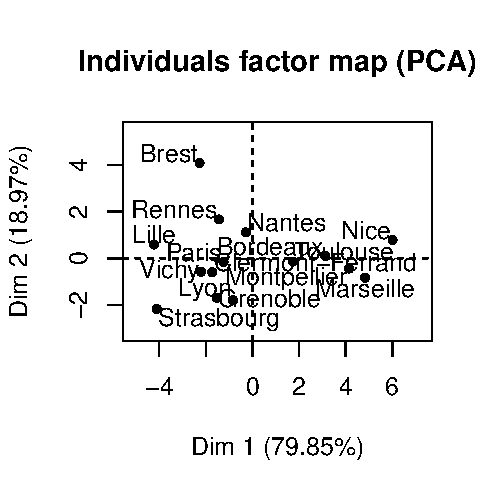
\includegraphics[width=\textwidth]{graphiques/beamer-unnamed-chunk-5-1} 
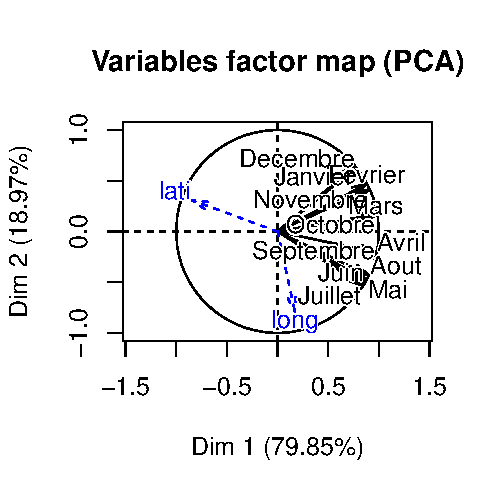
\includegraphics[width=\textwidth]{graphiques/beamer-unnamed-chunk-5-2} 

}



\end{knitrout}

colnames(temp)  
  
\end{frame}

\begin{frame}[containsverbatim]
  \frametitle{Graphique des  individus sur les deux premiers axes}

\begin{knitrout}\footnotesize
\definecolor{shadecolor}{rgb}{0.969, 0.969, 0.969}\color{fgcolor}\begin{kframe}
\begin{alltt}
\hlkwd{plot}\hlstd{(pca,}\hlkwc{choix} \hlstd{=} \hlstr{"ind"}\hlstd{)}
\end{alltt}
\end{kframe}

{\centering 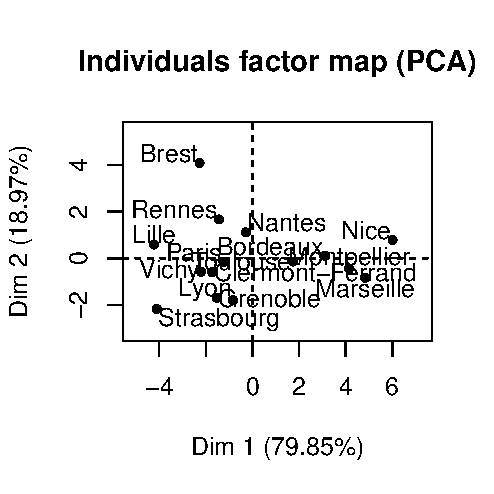
\includegraphics[width=\textwidth]{graphiques/beamer-unnamed-chunk-6-1} 

}



\end{knitrout}
\end{frame}



\begin{frame}[containsverbatim]
  \frametitle{Graphique des  individus sur les deux premiers axes}

\begin{knitrout}\footnotesize
\definecolor{shadecolor}{rgb}{0.969, 0.969, 0.969}\color{fgcolor}\begin{kframe}
\begin{alltt}
\hlkwd{cor}\hlstd{(pca}\hlopt{$}\hlstd{ind}\hlopt{$}\hlstd{coord[,}\hlnum{1}\hlopt{:}\hlnum{2}\hlstd{],temp[,}\hlkwd{c}\hlstd{(}\hlstr{"lati"}\hlstd{,}\hlstr{"long"}\hlstd{)])}
\end{alltt}
\begin{verbatim}
##             lati       long
## Dim.1 -0.8389348  0.1714839
## Dim.2  0.3064996 -0.7922192
\end{verbatim}
\end{kframe}
\end{knitrout}
\end{frame}

\begin{frame}[containsverbatim]
  \frametitle{Graphique des  individus sur les deux premiers axes}

  A partir des donn�es et des r�sultats de l'ACP, nous avons pu retrouver
  la lattitude et la longitude approximative.
  

\end{frame}

\end{document}


\documentclass{beamer}\usepackage[]{graphicx}\usepackage[]{color}
%% maxwidth is the original width if it is less than linewidth
%% otherwise use linewidth (to make sure the graphics do not exceed the margin)
\makeatletter
\def\maxwidth{ %
  \ifdim\Gin@nat@width>\linewidth
    \linewidth
  \else
    \Gin@nat@width
  \fi
}
\makeatother

\definecolor{fgcolor}{rgb}{0.345, 0.345, 0.345}
\newcommand{\hlnum}[1]{\textcolor[rgb]{0.686,0.059,0.569}{#1}}%
\newcommand{\hlstr}[1]{\textcolor[rgb]{0.192,0.494,0.8}{#1}}%
\newcommand{\hlcom}[1]{\textcolor[rgb]{0.678,0.584,0.686}{\textit{#1}}}%
\newcommand{\hlopt}[1]{\textcolor[rgb]{0,0,0}{#1}}%
\newcommand{\hlstd}[1]{\textcolor[rgb]{0.345,0.345,0.345}{#1}}%
\newcommand{\hlkwa}[1]{\textcolor[rgb]{0.161,0.373,0.58}{\textbf{#1}}}%
\newcommand{\hlkwb}[1]{\textcolor[rgb]{0.69,0.353,0.396}{#1}}%
\newcommand{\hlkwc}[1]{\textcolor[rgb]{0.333,0.667,0.333}{#1}}%
\newcommand{\hlkwd}[1]{\textcolor[rgb]{0.737,0.353,0.396}{\textbf{#1}}}%

\usepackage{framed}
\makeatletter
\newenvironment{kframe}{%
 \def\at@end@of@kframe{}%
 \ifinner\ifhmode%
  \def\at@end@of@kframe{\end{minipage}}%
  \begin{minipage}{\columnwidth}%
 \fi\fi%
 \def\FrameCommand##1{\hskip\@totalleftmargin \hskip-\fboxsep
 \colorbox{shadecolor}{##1}\hskip-\fboxsep
     % There is no \\@totalrightmargin, so:
     \hskip-\linewidth \hskip-\@totalleftmargin \hskip\columnwidth}%
 \MakeFramed {\advance\hsize-\width
   \@totalleftmargin\z@ \linewidth\hsize
   \@setminipage}}%
 {\par\unskip\endMakeFramed%
 \at@end@of@kframe}
\makeatother

\definecolor{shadecolor}{rgb}{.97, .97, .97}
\definecolor{messagecolor}{rgb}{0, 0, 0}
\definecolor{warningcolor}{rgb}{1, 0, 1}
\definecolor{errorcolor}{rgb}{1, 0, 0}
\newenvironment{knitrout}{}{} % an empty environment to be redefined in TeX

\usepackage{alltt}
\usetheme[compress]{Singapore}
\useoutertheme{miniframes}

% \documentclass{beamer}
%\usetheme{Warsaw}

% Pour les documents en francais...
	\usepackage[latin1]{inputenc}
	\usepackage[french]{babel}
	\usepackage[french]{varioref}

% Math�matiques
	\usepackage{amsmath}

% Caracteres speciaux suppl�mentaires
	\usepackage{latexsym,amsfonts}

% A documenter
	\usepackage{moreverb}

% Macros pour les paquets
	\usepackage{array}  			% N�cessaires pour les tableaux de la macro Excel.

% Outil suppl�mentaire pour les tableaux
	\usepackage{multirow}
	\usepackage{booktabs}
	\usepackage{xcolor} % alternating row colors in table, incompatible avec certains modules
	\usepackage{longtable}
	\usepackage{colortbl}

% Pour ins�rer des graphiques
	\usepackage{graphicx} 			% Graphique simples
	\usepackage{subfigure}			% Graphiques multiples

% Pour ins�rer des couleurs
	\usepackage{color}

% Rotation des objets et des pages
%	\usepackage{rotating}
%	\usepackage{lscape}

% Pour insrer du code source, LaTeX ou SAS par exemple.
	\usepackage{verbatim}
        \usepackage{moreverb}
	\usepackage{listings}
	\usepackage{fancyvrb}

%	\lstset{language=SAS,numbers=left}		% Par dfaut le listing est en SAS

% Pour ins�rer des hyperliens
  \usepackage{hyperref}

% American Psychological Association (for bibliographic references).
	\usepackage{apacite}

% Pour l'utilisation des macros
	\usepackage{xspace}

% Pour l'utilisation de notes en fin de document.
%	\usepackage{endnotes}

% Array
%	\usepackage{multirow}
%	\usepackage{booktabs}

% Rotation
%	\usepackage{rotating}

% En t�tes et pieds de pages
%	\usepackage{fancyhdr}
%	\usepackage{lastpage}


% Page layout

% By LaTeX commands
%\setlength{\oddsidemargin}{0cm}
%\setlength{\textwidth}{16cm}
%\setlength{\textheight}{24cm}
%\setlength{\topmargin}{-1cm}
%\setlength{\marginparsep}{0.2cm}

% fancyheader parameters
%\pagestyle{fancy}

%\fancyfoot[L]{{\small Formation \LaTeX, DEPP}}
%\fancyfoot[c]{}
%\fancyfoot[R]{{\small \thepage/\pageref{LastPage}}}

%\fancyhead[L]{}
%\fancyhead[c]{}
%\fancyhead[R]{}


% Pour ins�rer des dessins de Linux
\newcommand{\LinuxA}{\includegraphics[height=0.5cm]{Graphiques/linux.png}}
\newcommand{\LinuxB}{\includegraphics[height=0.5cm]{Graphiques/linux.png}\xspace}

% Macro pour les petits dessins pour les diff�rents OS.
\newcommand{\Windows}{\emph{Windows}\xspace}
\newcommand{\Mac}{\emph{Mac OS X}\xspace}
\newcommand{\Linux}{\emph{Linux}\xspace}
\newcommand{\MikTeX}{MiK\tex\xspace}

\newcommand{\df}{\emph{data.frame}\xspace}
\newcommand{\dfs}{\emph{data.frames}\xspace}
\newcommand{\liste}{\emph{list}\xspace}
\newcommand{\listes}{\emph{lists}\xspace}

\newcommand{\factor}{\emph{factor}\xspace}
\newcommand{\character}{\emph{character}\xspace}
\newcommand{\logical}{\emph{logical}\xspace}

\newcommand{\cad}{c'est-�-dire\xspace}

\newcommand{\hreff}[2]{\underline{\href{#1}{#2}\xspace}}


% Titre
\title{Introduction � R}
\author{Pascal Bessonneau}
%\institute{DEPP}
\date{06/2015}
\subtitle{Clustering}

\begin{knitrout}
\definecolor{shadecolor}{rgb}{0.969, 0.969, 0.969}\color{fgcolor}\begin{kframe}


{\ttfamily\noindent\itshape\color{messagecolor}{\#\# Loading required package: FactoMineR}}\end{kframe}
\end{knitrout}

\IfFileExists{upquote.sty}{\usepackage{upquote}}{}
\begin{document}

\begin{frame}
	\maketitle
\end{frame}

\begin{frame}
	\tableofcontents
\end{frame}

% Begin document %%%%%%%%%%%%%%%%%%%%%%%%%%%%%%%%%%%%%%%%%%%%%%%%%%%%%%%%%%%%%%%%%%%%%%%%%%%%%%%%%%

\section{Cluster}

\begin{frame}[containsverbatim]
	\frametitle{Le principe}

  Le principe est � partir des variables de calculer la distance entre individus
  et de grouper les individus les plus proches.
  
\end{frame}

\begin{frame}[containsverbatim]
	\frametitle{Temp�rature}

Nous utilisons toujours les donn�es sur la temp�rature.

\begin{knitrout}\footnotesize
\definecolor{shadecolor}{rgb}{0.969, 0.969, 0.969}\color{fgcolor}\begin{kframe}
\begin{alltt}
\hlstd{temp} \hlkwb{<-} \hlkwd{read.csv2}\hlstd{(}\hlstr{"data/temp.csv"}\hlstd{)}
\hlkwd{colnames}\hlstd{(temp)}
\end{alltt}
\begin{verbatim}
##  [1] "Ville"     "Janvier"   "Fevrier"  
##  [4] "Mars"      "Avril"     "Mai"      
##  [7] "Juin"      "Juillet"   "Aout"     
## [10] "Septembre" "Octobre"   "Novembre" 
## [13] "Decembre"  "lati"      "long"
\end{verbatim}
\end{kframe}
\end{knitrout}

\end{frame}

\begin{frame}[containsverbatim]
	\frametitle{Pr�paration des donn�es}

Dans ce cas il faut centrer et r�duire les donn�es pour �viter les probl�mes
de diff�rence d'unit�s.

\begin{knitrout}\footnotesize
\definecolor{shadecolor}{rgb}{0.969, 0.969, 0.969}\color{fgcolor}\begin{kframe}
\begin{alltt}
\hlstd{numerics} \hlkwb{<-} \hlkwd{sapply}\hlstd{(temp,is.numeric)}
\hlkwa{for} \hlstd{(ii} \hlkwa{in} \hlkwd{which}\hlstd{(numerics))}
  \hlstd{temp[[ii]]} \hlkwb{<-} \hlkwd{scale}\hlstd{(temp[[ii]])}
\end{alltt}
\end{kframe}
\end{knitrout}

\end{frame}

\begin{frame}[containsverbatim]
  \frametitle{Peut-on r�sumer les informations ?}

\begin{knitrout}\footnotesize
\definecolor{shadecolor}{rgb}{0.969, 0.969, 0.969}\color{fgcolor}\begin{kframe}
\begin{alltt}
\hlstd{hcpc} \hlkwb{<-} \hlkwd{HCPC}\hlstd{(temp[,}\hlnum{1}\hlopt{:}\hlnum{12}\hlstd{],}\hlkwc{nb.clust} \hlstd{=} \hlnum{3}\hlstd{)}
\end{alltt}


{\ttfamily\noindent\bfseries\color{errorcolor}{\#\# Error in FUN(data[x, , drop = FALSE], ...): 'x' doit �tre num�rique}}\end{kframe}

{\centering 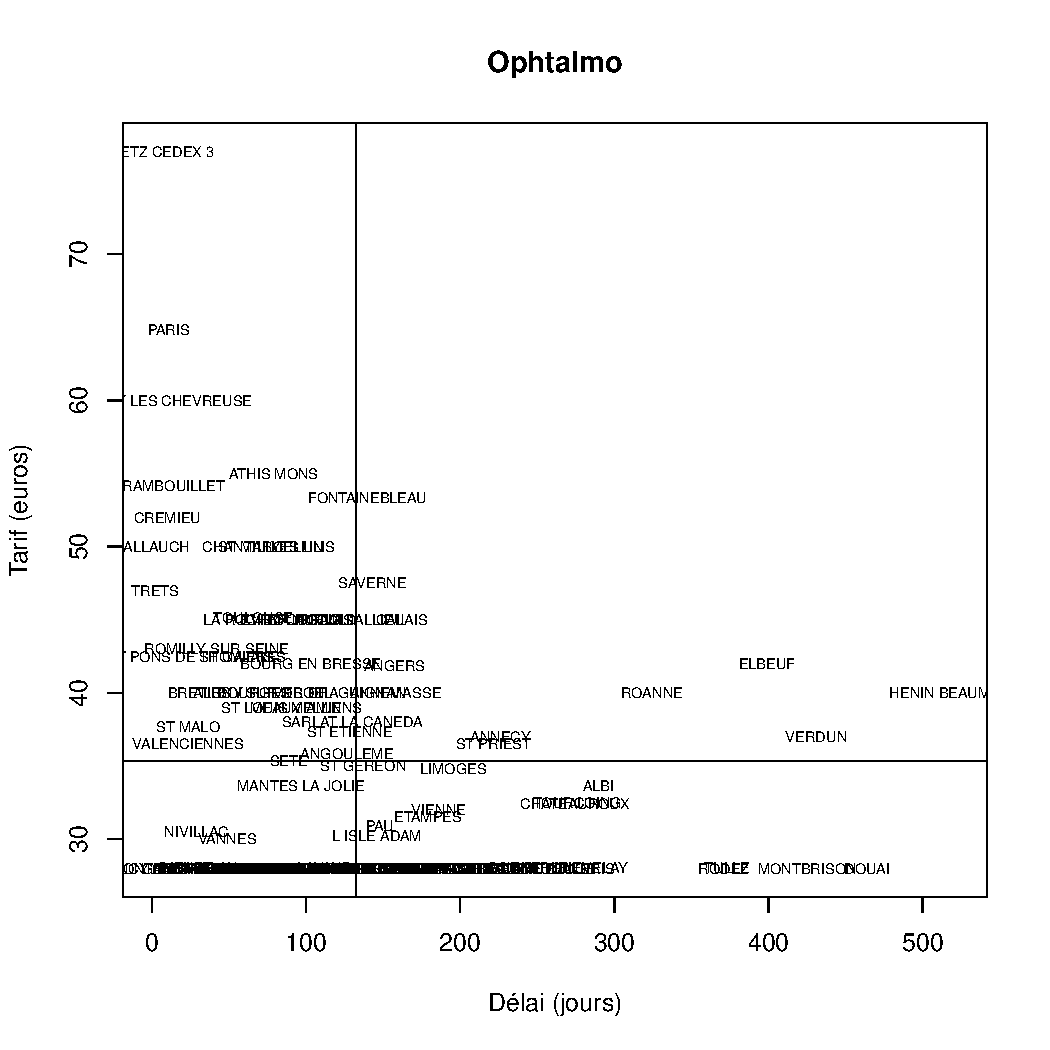
\includegraphics[width=\textwidth]{graphiques/beamer-unnamed-chunk-4-1} 

}



\end{knitrout}

\end{frame}


\begin{frame}[containsverbatim]
	\frametitle{R�sultats}

Nous pouvons voir � la longueur des branches de l'arbre quelles sont les villes
les plus proches les unes des autres. 

Apr�s l'algorithme nous propose une coupure optimale � 3 groupes.

\end{frame}

\begin{frame}[containsverbatim]
  \frametitle{R�sultats}

Nous avons 1 groupe qui r�unit les villes les plus au sud, un cluster
qui r�unit les villes de Bretagne au climat peu continental avec 
peu de variations entre les temp�ratures extr�mes et les villes au climat 
plus continental et situ� au nord de la Loire.
  
\end{frame}



\begin{frame}[containsverbatim]
  \frametitle{R�sultats}
  
  Le clustering fait partie des m�thodes de \emph{Machine Learning} qui 
  permettent d'analyser les comportements consomnateurs et du profilage
  des individus sur internet.

\end{frame}


  

\end{document}


\documentclass{beamer}\usepackage[]{graphicx}\usepackage[]{color}
%% maxwidth is the original width if it is less than linewidth
%% otherwise use linewidth (to make sure the graphics do not exceed the margin)
\makeatletter
\def\maxwidth{ %
  \ifdim\Gin@nat@width>\linewidth
    \linewidth
  \else
    \Gin@nat@width
  \fi
}
\makeatother

\definecolor{fgcolor}{rgb}{0.345, 0.345, 0.345}
\newcommand{\hlnum}[1]{\textcolor[rgb]{0.686,0.059,0.569}{#1}}%
\newcommand{\hlstr}[1]{\textcolor[rgb]{0.192,0.494,0.8}{#1}}%
\newcommand{\hlcom}[1]{\textcolor[rgb]{0.678,0.584,0.686}{\textit{#1}}}%
\newcommand{\hlopt}[1]{\textcolor[rgb]{0,0,0}{#1}}%
\newcommand{\hlstd}[1]{\textcolor[rgb]{0.345,0.345,0.345}{#1}}%
\newcommand{\hlkwa}[1]{\textcolor[rgb]{0.161,0.373,0.58}{\textbf{#1}}}%
\newcommand{\hlkwb}[1]{\textcolor[rgb]{0.69,0.353,0.396}{#1}}%
\newcommand{\hlkwc}[1]{\textcolor[rgb]{0.333,0.667,0.333}{#1}}%
\newcommand{\hlkwd}[1]{\textcolor[rgb]{0.737,0.353,0.396}{\textbf{#1}}}%

\usepackage{framed}
\makeatletter
\newenvironment{kframe}{%
 \def\at@end@of@kframe{}%
 \ifinner\ifhmode%
  \def\at@end@of@kframe{\end{minipage}}%
  \begin{minipage}{\columnwidth}%
 \fi\fi%
 \def\FrameCommand##1{\hskip\@totalleftmargin \hskip-\fboxsep
 \colorbox{shadecolor}{##1}\hskip-\fboxsep
     % There is no \\@totalrightmargin, so:
     \hskip-\linewidth \hskip-\@totalleftmargin \hskip\columnwidth}%
 \MakeFramed {\advance\hsize-\width
   \@totalleftmargin\z@ \linewidth\hsize
   \@setminipage}}%
 {\par\unskip\endMakeFramed%
 \at@end@of@kframe}
\makeatother

\definecolor{shadecolor}{rgb}{.97, .97, .97}
\definecolor{messagecolor}{rgb}{0, 0, 0}
\definecolor{warningcolor}{rgb}{1, 0, 1}
\definecolor{errorcolor}{rgb}{1, 0, 0}
\newenvironment{knitrout}{}{} % an empty environment to be redefined in TeX

\usepackage{alltt}
\usetheme[compress]{Singapore}
\useoutertheme{miniframes}

% \documentclass{beamer}
%\usetheme{Warsaw}

% Pour les documents en francais...
	\usepackage[latin1]{inputenc}
	\usepackage[french]{babel}
	\usepackage[french]{varioref}

% Math�matiques
	\usepackage{amsmath}

% Caracteres speciaux suppl�mentaires
	\usepackage{latexsym,amsfonts}

% A documenter
	\usepackage{moreverb}

% Macros pour les paquets
	\usepackage{array}  			% N�cessaires pour les tableaux de la macro Excel.

% Outil suppl�mentaire pour les tableaux
	\usepackage{multirow}
	\usepackage{booktabs}
	\usepackage{xcolor} % alternating row colors in table, incompatible avec certains modules
	\usepackage{longtable}
	\usepackage{colortbl}

% Pour ins�rer des graphiques
	\usepackage{graphicx} 			% Graphique simples
	\usepackage{subfigure}			% Graphiques multiples

% Pour ins�rer des couleurs
	\usepackage{color}

% Rotation des objets et des pages
%	\usepackage{rotating}
%	\usepackage{lscape}

% Pour insrer du code source, LaTeX ou SAS par exemple.
%	\usepackage{verbatim}
	\usepackage{listings}
	\usepackage{fancyvrb}

%	\lstset{language=SAS,numbers=left}		% Par dfaut le listing est en SAS

% Pour ins�rer des hyperliens
  \usepackage{hyperref}

% American Psychological Association (for bibliographic references).
	\usepackage{apacite}

% Pour l'utilisation des macros
	\usepackage{xspace}

% Pour l'utilisation de notes en fin de document.
%	\usepackage{endnotes}

% Array
%	\usepackage{multirow}
%	\usepackage{booktabs}

% Rotation
%	\usepackage{rotating}

% En t�tes et pieds de pages
%	\usepackage{fancyhdr}
%	\usepackage{lastpage}


% Page layout

% By LaTeX commands
%\setlength{\oddsidemargin}{0cm}
%\setlength{\textwidth}{16cm}
%\setlength{\textheight}{24cm}
%\setlength{\topmargin}{-1cm}
%\setlength{\marginparsep}{0.2cm}

% fancyheader parameters
%\pagestyle{fancy}

%\fancyfoot[L]{{\small Formation \LaTeX, DEPP}}
%\fancyfoot[c]{}
%\fancyfoot[R]{{\small \thepage/\pageref{LastPage}}}

%\fancyhead[L]{}
%\fancyhead[c]{}
%\fancyhead[R]{}

% Pour ins�rer des dessins de Linux
\newcommand{\LinuxA}{\includegraphics[height=0.5cm]{Graphiques/linux.png}}
\newcommand{\LinuxB}{\includegraphics[height=0.5cm]{Graphiques/linux.png}\xspace}

% Macro pour les petits dessins pour les diff�rents OS.
\newcommand{\Windows}{\emph{Windows}\xspace}
\newcommand{\Mac}{\emph{Mac OS X}\xspace}
\newcommand{\Linux}{\emph{Linux}\xspace}
\newcommand{\MikTeX}{MiK\tex\xspace}

\newcommand{\df}{\emph{data.frame}\xspace}
\newcommand{\dfs}{\emph{data.frames}\xspace}


\newcommand{\liste}{\emph{list}\xspace}
\newcommand{\factor}{\emph{factor}\xspace}
\newcommand{\character}{\emph{character}\xspace}
\newcommand{\logical}{\emph{logical}\xspace}

\newcommand{\cad}{c'est-�-dire\xspace}

\newcommand{\hreff}[2]{\underline{\href{#1}{#2}\xspace}}



% Titre
\title{Petite bibliographie}
\author{Pascal Bessonneau}
%\institute{DEPP}
\date{06/2015}



\IfFileExists{upquote.sty}{\usepackage{upquote}}{}
\begin{document}

\begin{frame}
	\maketitle
\end{frame}

\begin{frame}
	\tableofcontents
\end{frame}

% Begin document %%%%%%%%%%%%%%%%%%%%%%%%%%%%%%%%%%%%%%%%%%%%%%%%%%%%%%%%%%%%%%%%%%%%%%%%%%%%%%%%%%


\section{Documentation libre sur internet}

\begin{frame}[containsverbatim]
    \frametitle{Les manuels}

Comme �voqu� lors de la formation, le site \href{http://www.r-project.org/}{R-project.org} abrite les \href{http://cran.r-project.org/manuals.html}{manuels de R}. Ils sont une solide base sur R couvrant l'installation jusqu'� la cr�ation de paquets. On y trouve aussi la liste des fonctions R de base qui fait quelques milliers de pages.

Ils sont r�alis�s par le \og~noyau dur~\fg des d�veloppeurs de R. Toutefois, en dehors de la liste des fonctions de R, ils restent assez succints.

\end{frame}

\begin{frame}[containsverbatim]
    \frametitle{Les documents sugg�r�s\dots}

Ils se trouvent sur la page \href{http://cran.r-project.org/other-docs.html}{contributed documentation}. 

Les ouvrages pour d�buter les plus appr�ci�s sont g�n�ralement~:
\begin{itemize}
  \item R pour les d�butants, d'Emmanuel Paradis
	\item Brise Glace-R, traduction d'IcebreakeR.
	\item R pour les sociologues
	\item ...
\end{itemize}

Ces documents ont une approche bas�s sur les exemples essentiellement. Ils permettent de ma�triser les fonctions de base de R mais ne permettent g�n�ralement pas d'appr�hender tout le potentiel de R.

\end{frame}

\begin{frame}[containsverbatim]
    \frametitle{Les documents sugg�r�s\dots}

Un ouvrage offrant un plus de distance est l'ouvrage de Vincent Goulet.

Pour ceux qui ne redoutent pas l'anglais, la lecture des documents de J. Faraway et F. Harrell Jr. sont tr�s int�ressants notamment pour ceux int�ress�s par les m�thodes de r�gression.

Les documents de C. Genolini sont remarquables mais n�cessitent une certaine ma�trise de R.

\end{frame}

\begin{frame}[containsverbatim]
    \frametitle{Ouvrages sp�cialis�s}

D'autres documents sont plus sp�cifiques comme ceux sur l'�conom�trie, l'actuariat, ... Quelques r�f�rences suppl�mentaires~: 

\begin{itemize}
	\item Pour l'analyse de questionnaires conatifs et cognitifs, le site \href{http://personality-project.org/}{Personnality Project} qui abrite un ouvrage de tr�s bonne facture en cours de r�daction.
	\item Oeuvre du RUG Element-R, un \href{http://elementr.parisgeo.cnrs.fr/}{ouvrage} sur la cartographie en fran�ais
	\item L'ouvrage de G. Sanchez sur le \href{http://www.gastonsanchez.com/PLS_Path_Modeling_with_R.pdf}{PLS Path Modeling}
	\item TraMineR, pour l'analyse de trajectoires
	\item \dots
\end{itemize}

\end{frame}

\section{Ouvrages payants}

\begin{frame}[containsverbatim]
    \frametitle{Statistiques}

Dans cette section sont indiqu�s quelques livres int�ressants avec un bref commentaire. L'opinion des formateurs n'�tant pas parole d'�vangiles vous pourrez trouver des informations sur les livres cit�s ci-dessous sur la page \href{http://www.r-project.org/doc/bib/R-books.html}{Books} de R.

Couvrant une large palette de m�thodes statistiques, l'ouvrage de \citeA{Crawley2013} est un livre tr�s int�ressant qui permet de trouver rapidement comment r�aliser ces m�thodes avec R.

Le livre de \citeA{Albert2012} illustre diff�rents m�thodes � travers quelques exemples. N�anmoins sa qualit� est un peu en retrait par rapport au livre de \citeA{Crawley2013}.

L'ouvrage de \citeA{Dalgaard2008} est un livre d'initiation � la fois aux statistiques (simples) et � R. L'auteur fait partie des d�veloppeurs de R. Il est didactique et int�ressant. 

\end{frame}

\begin{frame}[containsverbatim]
    \frametitle{Langages et programmation}

Le livre de \citeA{Gentleman2009} est un livre remarquable qui couvre le niveau d�butant � avanc�. Toutefois son approche est plus informatique que statistique. Il est possible que sa lecture soit d�routante si on a pas de bonnes connaissances en programmation.

Le livre de \citeA{Chambers2008} est int�ressant et s'adresse aussi � un public interm�diaire et averti. Il couvre notamment la manipulation de donn�es.

L'ouvrage de \citeA{Genolini2010} est pr�cieux. Toutefois il s'adresse � un public averti. Il s'agit de la version papier de documents librement t�l�chargeables sur le web (voir partie pr�c�dente). Pour les parisiens, l'auteur est dans le RUG Semin-R.

\end{frame}

\begin{frame}[containsverbatim]
    \frametitle{Langages et programmation}

Le livre de \citeA{Matloff2011} est un must-have. Remarquable, il couvre les possibilit�s offertes par R en tant que langage fonctionnel. Il couvre aussi le d�bogage des fonctions R ainsi que la programmation objet. Mais il s'adresse � un public venant plus de l'informatique que des statistiques.

Les \emph{blue book} de \citeA{Ripley2002}, illustrant des exemples statistiques avec R et le \emph{yellow book} de \cite{Ripley2000} sont des classiques. Le \emph{yellow book} ne s'int�resse qu'au langage lui-m�me. L'int�r�t de ces livres est surtout historique.

Le must-have est le livre de \cite{Wickham2015}

\end{frame}

\begin{frame}[containsverbatim]
    \frametitle{Graphiques}

Le must-have est le livre de \cite{Murrell2011}. Il couvre toutes les possibilit�s graphiques de R. Attention � bien acheter la deuxi�me version infiniment plus int�ressante car elle couvre les graphiques traditionnels de R (pr�sent�s lors de la formation), le paquet \textit{grid} et les packages \textit{Lattice} et \textit{ggplot2}.

\end{frame}

\begin{frame}[containsverbatim]
    \frametitle{Graphiques}

Le package \emph{Lattice} permet des r�aliser des graphiques avanc�s. Il permet notamment d'automatiser la cr�ation de graphiques par variables cat�gorielles, faire des tableaux de graphiques aisement, ... Ce paquet d�velop� par un membre du R Core est en perte de vitesse. Son concurrent est \textit{ggplot2} qui pr�sente les m�mes fonctionnalit�s avec une qualit� graphique sup�rieure et plus d'options. 

Le paquet \textit{Lattice} a son livre \cite{Sarkar2008} comme ggplot2\cite{Wickham2009}.

Le livre de \citeA{Wickham2009} est le manuel du package. Une approche plus didactique est propos� dans le livre de \cite{Chang2012}. Bas� sur des exemples, il est pratique pour d�buter mais l'ouvrage de \cite{Wickham2009} reste la r�f�rence du \emph{langage} de \emph{ggplot2}. 

A noter que le paquet ggplot2, a �t� d�velopp� dans l'esprit du livre de \citeA{Wilkinson2005}. Ce livre est tr�s int�ressant pour acqu�rir les bonnes pratiques en mati�re de graphiques.

\end{frame}

\begin{frame}[containsverbatim]
    \frametitle{R�gression}

Les ouvrages de \citeA{Harrell2001}, \cite{Faraway2005} et \citeA{Faraway2006} sont assez anciens. Mais ce sont d'excellents livres de r�f�rence et qui couvrent les r�gressions lin�aires, logistique, ... Outre l'utilisation de R, ce sont d'excellents livres concernant la r�gression\footnote{Ils sont assez techniques}.

Un excellent livre en fran�ais sur la r�gression lin�aire avec R~ de \cite{Cornillon2011} est paru chez Springer. Il m�le th�orie et pratique avec R.

Plus complexe, l'ouvrage de \citeA{Sheather2009} est tr�s int�ressant.

\end{frame}

\begin{frame}[containsverbatim]
    \frametitle{Applications particuli�res}

Dans \cite{Lumley2010}, le package \emph{survey} de l'auteur est d�crit � travers des exemples de sondage simple, stratifi� et � plusieurs degr�s. Le probl�me est que l'auteur a �normement travaill� sur son package et beaucoup de fonctionnalit�s de son package ne sont pas pr�sents dans le livre.

Le livre de r�f�rence pour l'analyse de donn�es spatiales et la cartographie est l'ouvrage de \citeA{Bivand2008}.

Le livre de \citeA{Robert2010} est tr�s int�ressant et illustre bien les m�thodes Monte-Carlo dans R.

Pour les analyses longitudinales, l'ouvrage de \citeA{Long2012} offre beaucoup d'informations pour ceux qui sont int�ress�s par les mesures r�p�t�es et les �tudes longitudinales.

\end{frame}

\begin{frame}[containsverbatim]
    \frametitle{Applications particuli�res}

Le livre d'\citeA{Albert2009} couvre le probl�me des statistiques bay�siennes et la fa�on de r�aliser les calculs dans R. 

Le livre de \citeA{Pinheiro2000} est un classique... Un must-have pour tous ceux qui veulent travailler avec des mod�les mixtes sous R. Le livre est bas� sur le paquet \emph{nlme}. Un package plus r�cent \emph{lme4} existe. Les deux paquets pr�sente beaucoup de similitudes donc... Quelques nouveaut�s sont pr�sentes \emph{lme4} mais dont le temps d'ex�cution est beaucoup plus lent que \emph{nlme}.

Un livre \cite{Zuur2009} plus r�cent, orient� �cologie mais d'une grande qualit�, couvre les mod�les mixtes, hi�rarchiques, les GLMs, ... 

\end{frame}

\begin{frame}[containsverbatim]
    \frametitle{Applications particuli�res}

Le livre de \citeA{McCallum2012} est tr�s sp�cifique. Il traite de la parall�lisation 
des calculs sous R. Il permet de d�couvrir les diff�rentes possibilit�s pour faire 
du calcul parall�le sous R. Sa parution est juste ant�rieure � l'int�gration du 
package \textit{parallel} par d�faut dans R. Par cons�quent il couvre la version 
beta de \textit{parallel}. Si la parall�lisation des calculs est tr�s ais� sous 
GNU/Linux, il traite aussi des m�thodes plus complexes (disponibles sous Windows 
et sous GNU/Linux) pour faire du calcul parall�le. 

Pour l'analyse de questionnaire, un livre est disponible et a �t� �crit par un 
grand statisticien fran�ais. Il s'agit de l'ouvrage de \citeA{Falissard2011}. Il 
s'adresse � un public de niveau d�butant � mod�r�. On y trouve les codes pour 
r�aliser des analyses factorielles (� l'anglaise, sur variables latentes) et la 
validation de questionnaire. Il est assez orient� vers la m�decine, l'auteur 
�tant directeur d'un laboratoire de recherche en psychiatrie. 

\end{frame}

\begin{frame}[containsverbatim]
    \frametitle{Applications particuli�res}

Pour le paquet FactoMineR, pour l'analyse de donn�es � la fran�aise, deux livres sont disponibles.

Le premier sur les m�thodes traditionnnelles (ACP, ACM, \dots) \cite{Husson2009} 
et le second sur l'analyse factorielle multiple et l'analyse de donn�es mixtes 
\cite{Pages2015}.



\end{frame}

\begin{frame}[containsverbatim]
    \frametitle{Citations}

\bibliographystyle{apacite}
\bibliography{articles}

\end{frame}

\end{document}


\end{document}
